\documentclass{Configuration_Files/PoliMi3i_thesis}

%------------------------------------------------------------------------------
%	REQUIRED PACKAGES AND  CONFIGURATIONS
%------------------------------------------------------------------------------

% CONFIGURATIONS
\usepackage{parskip} % For paragraph layout
\usepackage{setspace} % For using single or double spacing
\usepackage{emptypage} % To insert empty pages
\usepackage{multicol} % To write in multiple columns (executive summary)
\setlength\columnsep{15pt} % Column separation in executive summary
\setlength\parindent{0pt} % Indentation
\raggedbottom  

% PACKAGES FOR TITLES
\usepackage{titlesec}
% \titlespacing{\section}{left spacing}{before spacing}{after spacing}
\titlespacing{\section}{0pt}{3.3ex}{2ex}
\titlespacing{\subsection}{0pt}{3.3ex}{1.65ex}
\titlespacing{\subsubsection}{0pt}{3.3ex}{1ex}
\usepackage{color}

% PACKAGES FOR LANGUAGE AND FONT
\usepackage[english]{babel} % The document is in English  
\usepackage[utf8]{inputenc} % UTF8 encoding
\usepackage[T1]{fontenc} % Font encoding
\usepackage[11pt]{moresize} % Big fonts

% PACKAGES FOR IMAGES
\usepackage{graphicx}
\usepackage{transparent} % Enables transparent images
\usepackage{eso-pic} % For the background picture on the title page
\usepackage{subfig} % Numbered and caption subfigures using \subfloat.
\usepackage{tikz} % A package for high-quality hand-made figures.
\usetikzlibrary{}
\graphicspath{{./Images/}} % Directory of the images
\usepackage{caption} % Coloured captions
\usepackage{xcolor} % Coloured captions
\usepackage{amsthm,thmtools,xcolor} % Coloured "Theorem"
\usepackage{float}

% STANDARD MATH PACKAGES
\usepackage{amsmath}
\usepackage{amsthm}
\usepackage{amssymb}
\usepackage{amsfonts}
\usepackage{bm}
\usepackage[overload]{empheq} % For braced-style systems of equations.
\usepackage{fix-cm} % To override original LaTeX restrictions on sizes

% PACKAGES FOR TABLES
\usepackage{tabularx}
\usepackage{longtable} % Tables that can span several pages
\usepackage{colortbl}
\usepackage{multirow}
\usepackage{changepage}

% PACKAGES FOR ALGORITHMS (PSEUDO-CODE)
\usepackage{algorithm}
\usepackage{algorithmic}

% PACKAGES FOR REFERENCES & BIBLIOGRAPHY
\usepackage[colorlinks=true,linkcolor=black,anchorcolor=black,citecolor=black,filecolor=black,menucolor=black,runcolor=black,urlcolor=black]{hyperref} % Adds clickable links at references
\usepackage{cleveref}
\usepackage[square, numbers, sort&compress]{natbib} % Square brackets, citing references with numbers, citations sorted by appearance in the text and compressed
\bibliographystyle{abbrvnat} % You may use a different style adapted to your field

% OTHER PACKAGES
\usepackage{pdfpages} % To include a pdf file
\usepackage{afterpage}
\usepackage{lipsum} % DUMMY PACKAGE
\usepackage{fancyhdr} % For the headers
\fancyhf{}

% Manually added

% Input of configuration file. Do not change config.tex file unless you really know what you are doing. 
% Define blue color typical of polimi
\definecolor{bluepoli}{cmyk}{0.4,0.1,0,0.4}

% Custom theorem environments
\declaretheoremstyle[
  headfont=\color{bluepoli}\normalfont\bfseries,
  bodyfont=\color{black}\normalfont\itshape,
]{colored}

% Set-up caption colors
\captionsetup[figure]{labelfont={color=bluepoli}} % Set colour of the captions
\captionsetup[table]{labelfont={color=bluepoli}} % Set colour of the captions
\captionsetup[algorithm]{labelfont={color=bluepoli}} % Set colour of the captions

\theoremstyle{colored}
\newtheorem{theorem}{Theorem}[chapter]
\newtheorem{proposition}{Proposition}[chapter]

% Enhances the features of the standard "table" and "tabular" environments.
\newcommand\T{\rule{0pt}{2.6ex}}
\newcommand\B{\rule[-1.2ex]{0pt}{0pt}}

% Pseudo-code algorithm descriptions.
\newcounter{algsubstate}
\renewcommand{\thealgsubstate}{\alph{algsubstate}}
\newenvironment{algsubstates}
  {\setcounter{algsubstate}{0}%
   \renewcommand{\STATE}{%
     \stepcounter{algsubstate}%
     \Statex {\small\thealgsubstate:}\space}}
  {}

% New font size
\newcommand\numfontsize{\@setfontsize\Huge{200}{60}}

% Title format: chapter
\titleformat{\chapter}[hang]{
\fontsize{50}{20}\selectfont\bfseries\filright}{\textcolor{bluepoli} \thechapter\hsp\hspace{2mm}\textcolor{bluepoli}{|   }\hsp}{0pt}{\huge\bfseries \textcolor{bluepoli}
}

% Title format: section
\titleformat{\section}
{\color{bluepoli}\normalfont\Large\bfseries}
{\color{bluepoli}\thesection.}{1em}{}

% Title format: subsection
\titleformat{\subsection}
{\color{bluepoli}\normalfont\large\bfseries}
{\color{bluepoli}\thesubsection.}{1em}{}

% Title format: subsubsection
\titleformat{\subsubsection}
{\color{bluepoli}\normalfont\large\bfseries}
{\color{bluepoli}\thesubsubsection.}{1em}{}

% Shortening for setting no horizontal-spacing
\newcommand{\hsp}{\hspace{0pt}}

\makeatletter
% Renewcommand: cleardoublepage including the background pic
\renewcommand*\cleardoublepage{%
  \clearpage\if@twoside\ifodd\c@page\else
  \null
  \AddToShipoutPicture*{\BackgroundPic}
  \thispagestyle{empty}%
  \newpage
  \if@twocolumn\hbox{}\newpage\fi\fi\fi}
\makeatother

%For correctly numbering algorithms
\numberwithin{algorithm}{chapter}

%----------------------------------------------------------------------------
%	NEW COMMANDS DEFINED
%----------------------------------------------------------------------------

% EXAMPLES OF NEW COMMANDS
\newcommand{\bea}{\begin{eqnarray}} % Shortcut for equation arrays
\newcommand{\eea}{\end{eqnarray}}
\newcommand{\e}[1]{\times 10^{#1}}  % Powers of 10 notation

%----------------------------------------------------------------------------
%	ADD YOUR PACKAGES (be careful of package interaction)
%----------------------------------------------------------------------------

%----------------------------------------------------------------------------
%	ADD YOUR DEFINITIONS AND COMMANDS (be careful of existing commands)
%----------------------------------------------------------------------------

%----------------------------------------------------------------------------
%	BEGIN OF YOUR DOCUMENT
%----------------------------------------------------------------------------

\begin{document}

\fancypagestyle{plain}{%
\fancyhf{} % Clear all header and footer fields
\fancyhead[RO,RE]{\thepage} %RO=right odd, RE=right even
\renewcommand{\headrulewidth}{0pt}
\renewcommand{\footrulewidth}{0pt}}

%----------------------------------------------------------------------------
%	TITLE PAGE
%----------------------------------------------------------------------------

\pagestyle{empty} % No page numbers
\frontmatter % Use roman page numbering style (i, ii, iii, iv...) for the preamble pages

\puttitle{
	title=MacroTracker, % Title of the thesis
	name=Alessandro Sironi \\ \\ Tommaso Sprocati, % Author Name and Surname
	course=Design and Implementation of Mobile Applications, % Study Programme (in Italian)
	ID  = 10680296-232828 \\ 10666918 - 232789,  % Student ID number (numero di matricola)
	academicyear={2022-23},  % Academic Year
	advisor=Luciano Baresi,
} % These info will be put into your Title page 

\setcounter{page}{1} % Set page counter to 1

%----------------------------------------------------------------------------
%	LIST OF CONTENTS/FIGURES/TABLES/SYMBOLS
%----------------------------------------------------------------------------

% TABLE OF CONTENTS
\thispagestyle{empty}
\tableofcontents % Table of contents 
\thispagestyle{empty}
\cleardoublepage

%-------------------------------------------------------------------------
%	THESIS MAIN TEXT
%-------------------------------------------------------------------------
% In the main text of your thesis you can write the chapters in two different ways:
%
%(1) As presented in this template you can write:
%    \chapter{Title of the chapter}
%    *body of the chapter*
%
%(2) You can write your chapter in a separated .tex file and then include it in the main file with the following command:
%    \chapter{Title of the chapter}
%    \input{chapter_file.tex}
%
% Especially for long thesis, we recommend you the second option.

\addtocontents{toc}{\vspace{2em}} % Add a gap in the Contents, for aesthetics
\mainmatter % Begin numeric (1,2,3...) page numbering

% --------------------------------------------------------------------------
% NUMBERED CHAPTERS % Regular chapters following
% --------------------------------------------------------------------------

\chapter{Introduction}
\section{Project Description}
The mobile application developed is called \textbf{MacroTracker}. The application consists in a fitness-focused project that allows athletes to track and log food intake and macro-nutrients in order to compile statistics of one's eating habits.
Therefore, to help the user achieve their fitness goals by collecting quantitative data on their diet. 
The main functionalities are:
\begin{itemize}
    \item The ability for the user to enter their own \textbf{nutritional goals}. 
    \item The \textbf{tracking} of the daily diet, aided by the possibility to insert the consumed food through either a \textbf{manual insertion}, or the \textbf{scan of a product's barcode}. 
    Regarding this function, we identified an open-source API service called \textbf{\textit{OpenFoodFacts}} (\url{https://it.openfoodfacts.org}) that contains a large dataset of off-the-shelf food products information. 
    \item The ability for the user to receive a \textbf{notification reminder} to help them remember to log their food intake of the day.
    \item Showing useful information through \textbf{graphs} to monitor progress. 
    \item The integration with \textbf{Apple HealthKit} in order to take advantage of the ecosystem to store data, so that it is available from other apps. 
\end{itemize}
The project has been developed in \textbf{Flutter}. The supported devices are phones and tablets, both iOS and Android devices. The main focus has been placed on iOS and iPadOS devices.
\section{Features}
\subsection{Diary Summary of the day}
The user can see at a glance the day's situation regarding their food intake and diet and, via a calendar view, can change the date to inspect other days' situations. 
\subsection{Quick add for water and coffee assumption}
Through easy and quick buttons, the user can add or remove a water or coffee assumption for the day. 
\subsection{Goal setting}
The user can easily modify their diet goals to reflect the changes in their training and lifestyle. The Goal page presents to the user also a few information and tips to help the athlete take conscious decision about their diet goals. 
\subsection{Saving common foods for quick adds}
The user can create ad-hoc common foods that are recurrent in their diet for a quicker add in the daily assumption. 
\subsection{Modify an insertion}
The user can always modify or delete an insertion, whether if they decide to change the values or if they input data by mistake. 
\subsection{Multiple Device Synchronization}
By logging in with the same account in multiple devices, the user has all the data synchronized via the cloud, so that they can update their data from multiple devices and have them synchronized.
\subsection{Notification reminder}
The user will be reminded to use the app through a scheduled notification that takes place near the end of the day. The notification is scheduled only if the user actively uses the app, so that if they decide to pause the use of the app, they're not overloaded with notifications.
\section{Purpose}
The purpose of this document is to provide a description of the architecture and design of the application, focusing on the architecture adopted and the decisions that drove the final design. 
%\section{Definitions, Acronyms, Abbreviations}
%\section{Reference Documents and Websites}
%\section{Document Structure}

\chapter{Architectural Design}
\section{Overview}
MacroTracker is a Flutter application, developed for iOS and iPadOS devices, with support for Android devices. 
Its architecture relies on Firebase as a safe and secure \textbf{backend} for authenticating the users and store the users' data. \\
The food database to which the application requests the food nutritional values is \textbf{OpenFoodFacts} - \url{https://it.openfoodfacts.org}. The \textit{open data} and \textit{open source} database offers APIs that let developers take advantage of the vast amount of labeled food products. \\
At last, the app has been thought out to interact with Apple Health's ecosystem. The values saved in the app are made available as Apple Health entries on supported devices. 
\subsection{Authentication}
MacroTracker logins and signs up users via Firebase Authentication (\url{https://firebase.google.com/docs/auth}). The supported sign-in method is \textbf{Email/Password}. Users are assigned an unique identifier, that will be used in the Firestore Database for identifying the user's collection. 
\subsection{Data Management}
The application relies on an online and in-cloud database: Cloud Firestore (\url{https://firebase.google.com/docs/firestore}). 
The database contains data related to the user's basic information, the user's nutritional goals, the food entries for each day, as well as the diet foods saved for quicker adds. 
\subsection{Data Structure}
The database structure is defined as follows.
\begin{figure}[H]
  \centering
  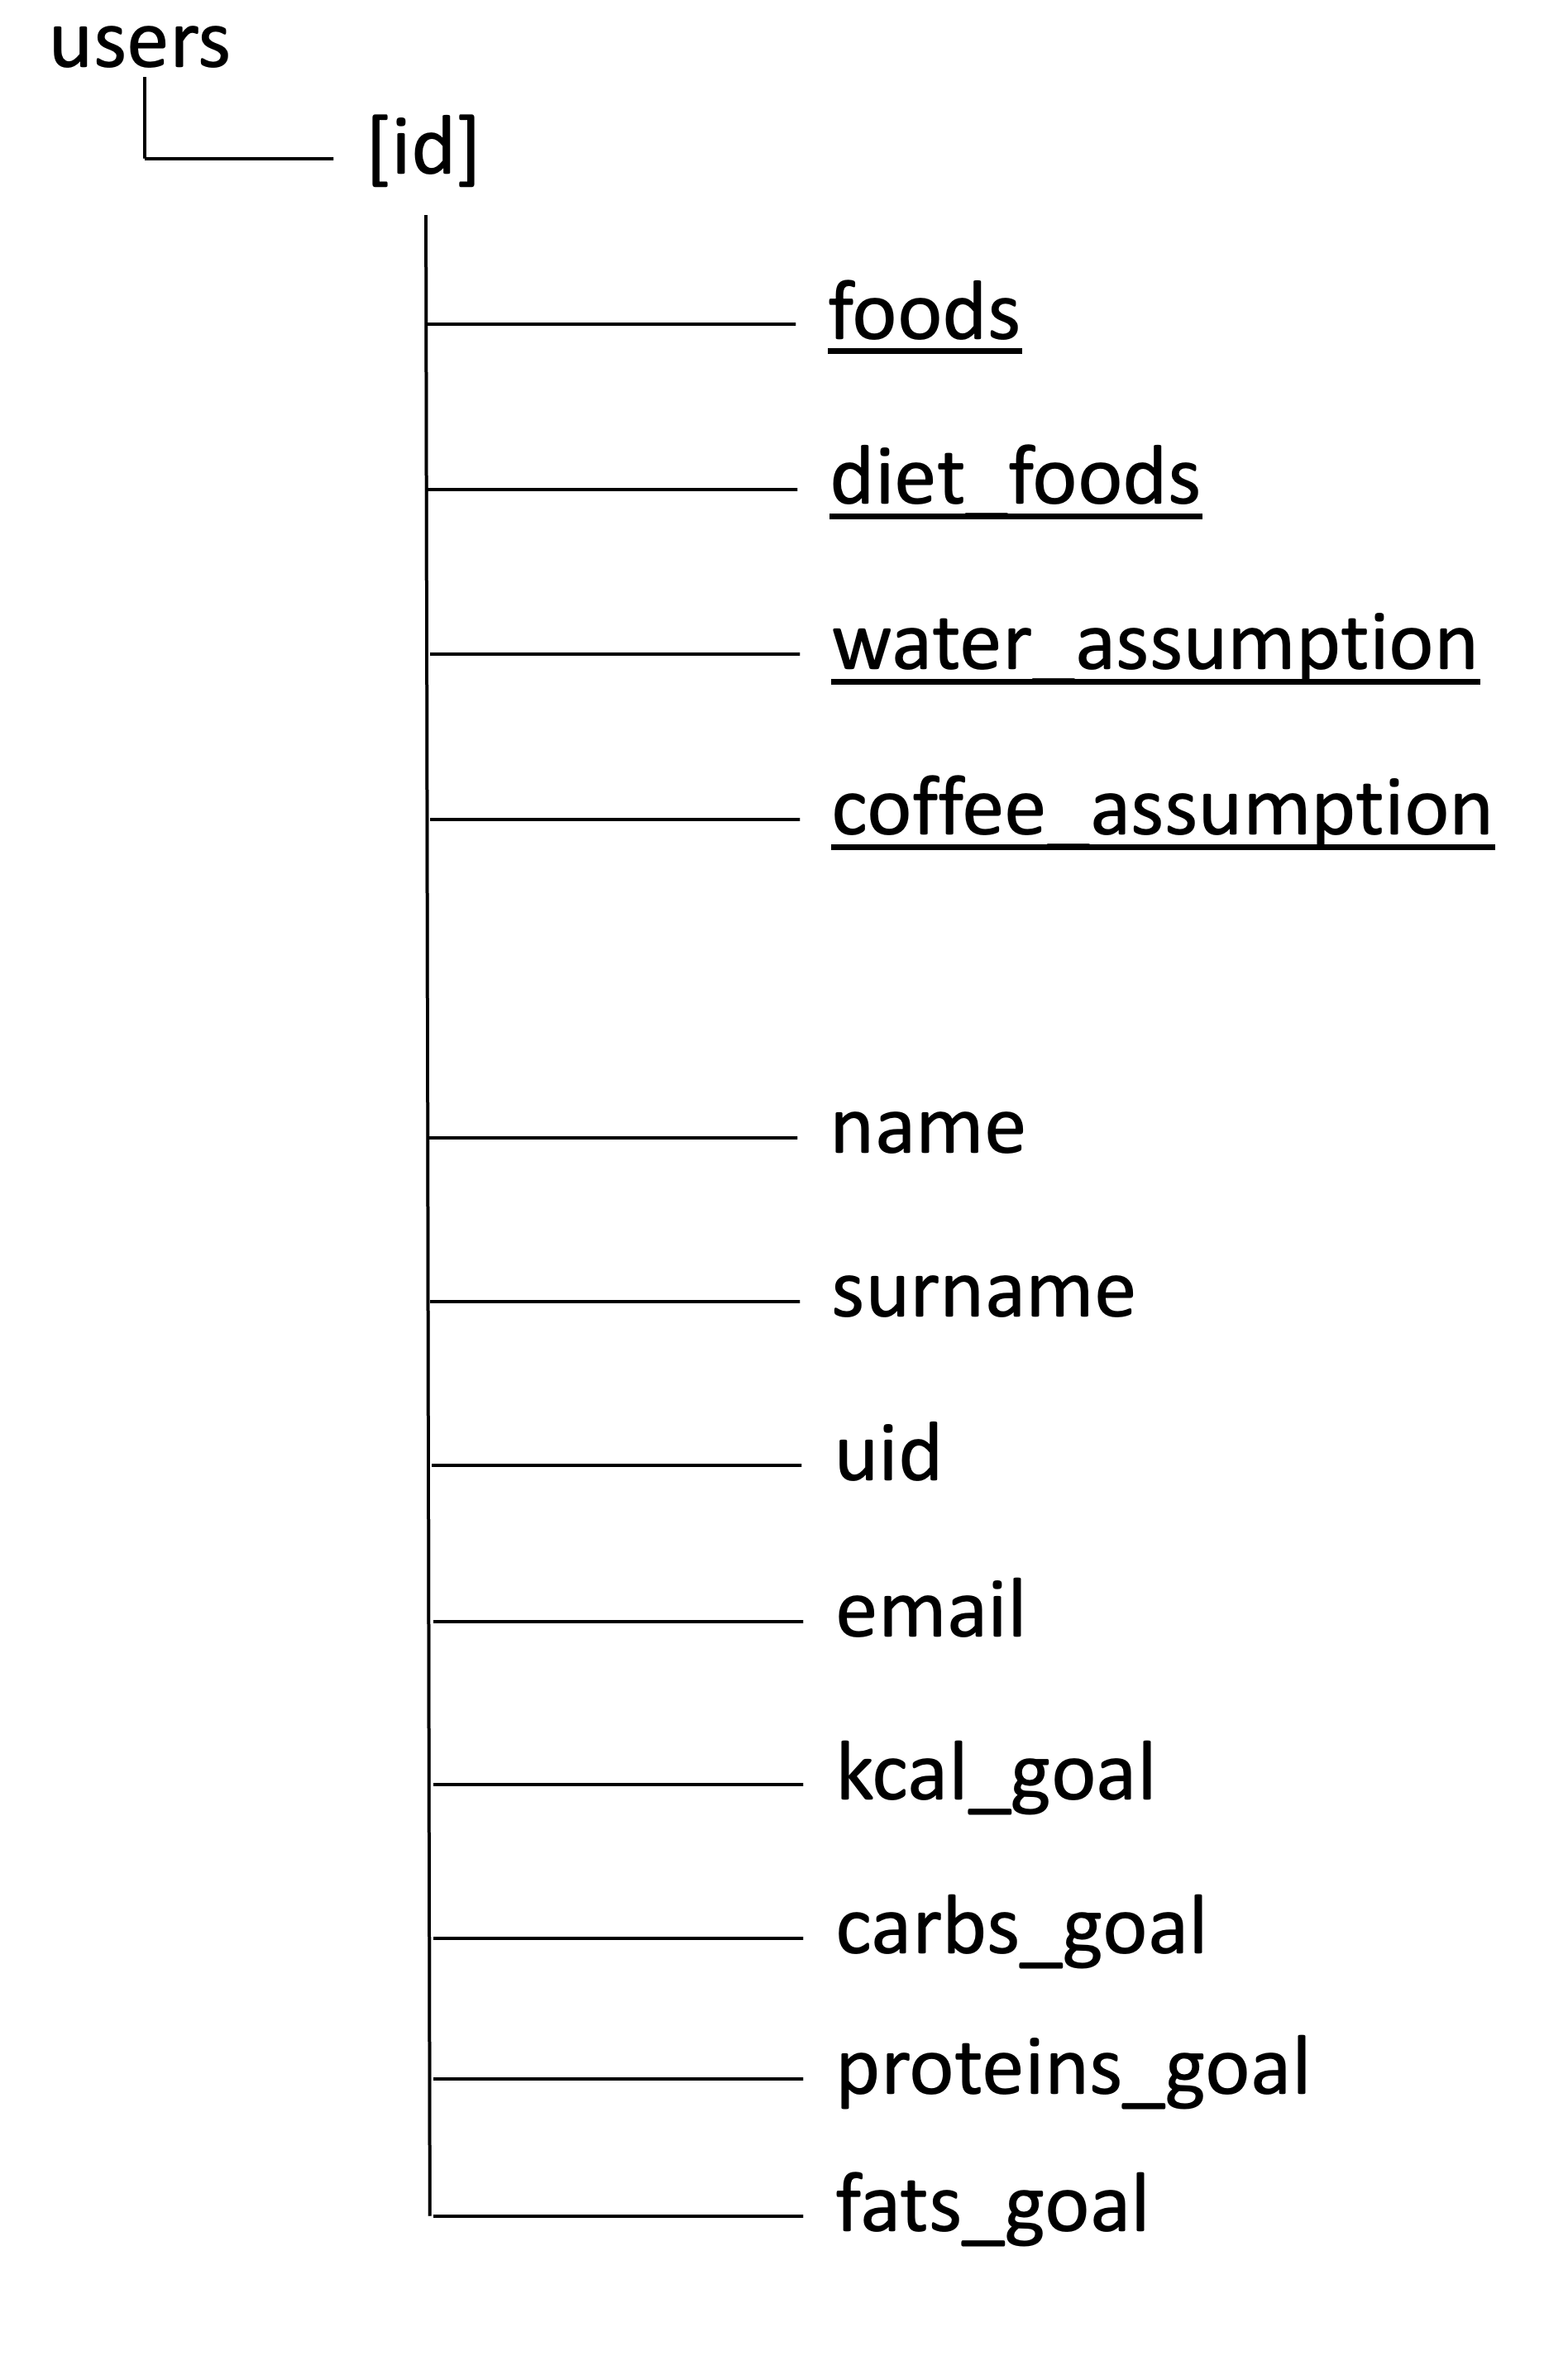
\includegraphics[scale=0.25]{Images/db_structure.png}
  \caption{Database structure}
\end{figure}
\begin{figure}[H]
  \centering
  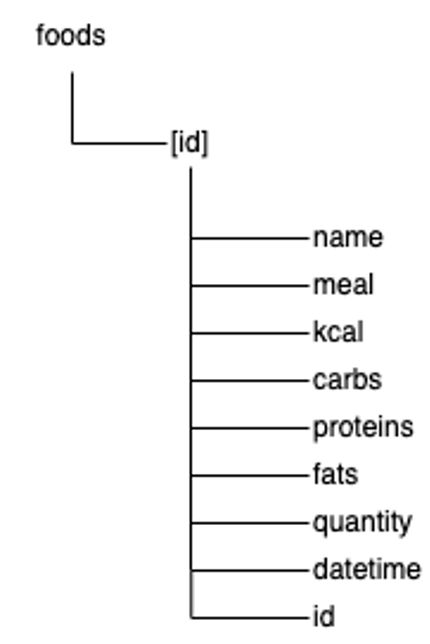
\includegraphics[scale=0.6]{Images/foods_db.png}
  \caption{Foods Database structure}
\end{figure}
Note that underlined elements in the structure represent sub-collections, whereas the non-underlined entries are fields. 
Each user has access to its own collection, identifiable by the UID assigned by Firebase Authentication. 
Every user has the ability to log its daily diet, favorite foods, the amount of glasses of water and coffee drunk each day. The user can then retrieve old data to check the progress made, and-or to adjust mistaken entries. 
\subsection{Food Data retrieval}
MacroTracker takes advantage of the largest open-source and open-data food database, that contains more than 2.7 million of products from 150 countries. 
The user has the ability to find in the database nutrition facts of off-the-shelf products via a barcode scan. The database then returns the nutritional info of the desired product. 
Open Food Facts provides an API to interact with the database (\url{https://pub.dev/packages/openfoodfacts}).
\section{Architectural Style and Patterns}
\subsection{Two-Tier Architecture, Model and View-Controller}
The application has been thought out to use a two-tier architecture. The client portion is the app itself whereas the "Server" is itself the cloud-provided back-end of Firebase. \\
The pattern chosen to organize the project itself is "View-Controller", as most of the data manipulation, creation and retrieval is handled through Firebase; widgets are built dynamically given the retrieved data.
\section{Widgets}
As a Flutter application, MacroTracker is built by several widgets that build the correct view and respond to the user's input. 
\subsection{Main screens and Navigation}
The application has some main screens that are accessible from each other via a bottom navigation bar, present in (almost) all the screens:
\begin{itemize}
    \item \textbf{Diary}: This is the main view for the application, and - provided the user is logged in - is the first screen shown at the start of the app.
    \item \textbf{Goal}: This page allows the user to set their kcal, carbs, proteins and fats goals. It also provides some basic information to guide the user through their decision. 
    \item \textbf{Add}: Represented by a plus icon, this page lets the user make a new food entry by scanning a barcode, adding manually or from the diet. 
    \item \textbf{Diet}: This view shows all the foods that the user has saved, to be logged more easily. The foods can be filtered, modified and added from this view.
    \item \textbf{Profile}: In this view, the user can modify their personal data, switch to dark/light mode and log out. 
\end{itemize}
\begin{figure}[H]
  \centering
  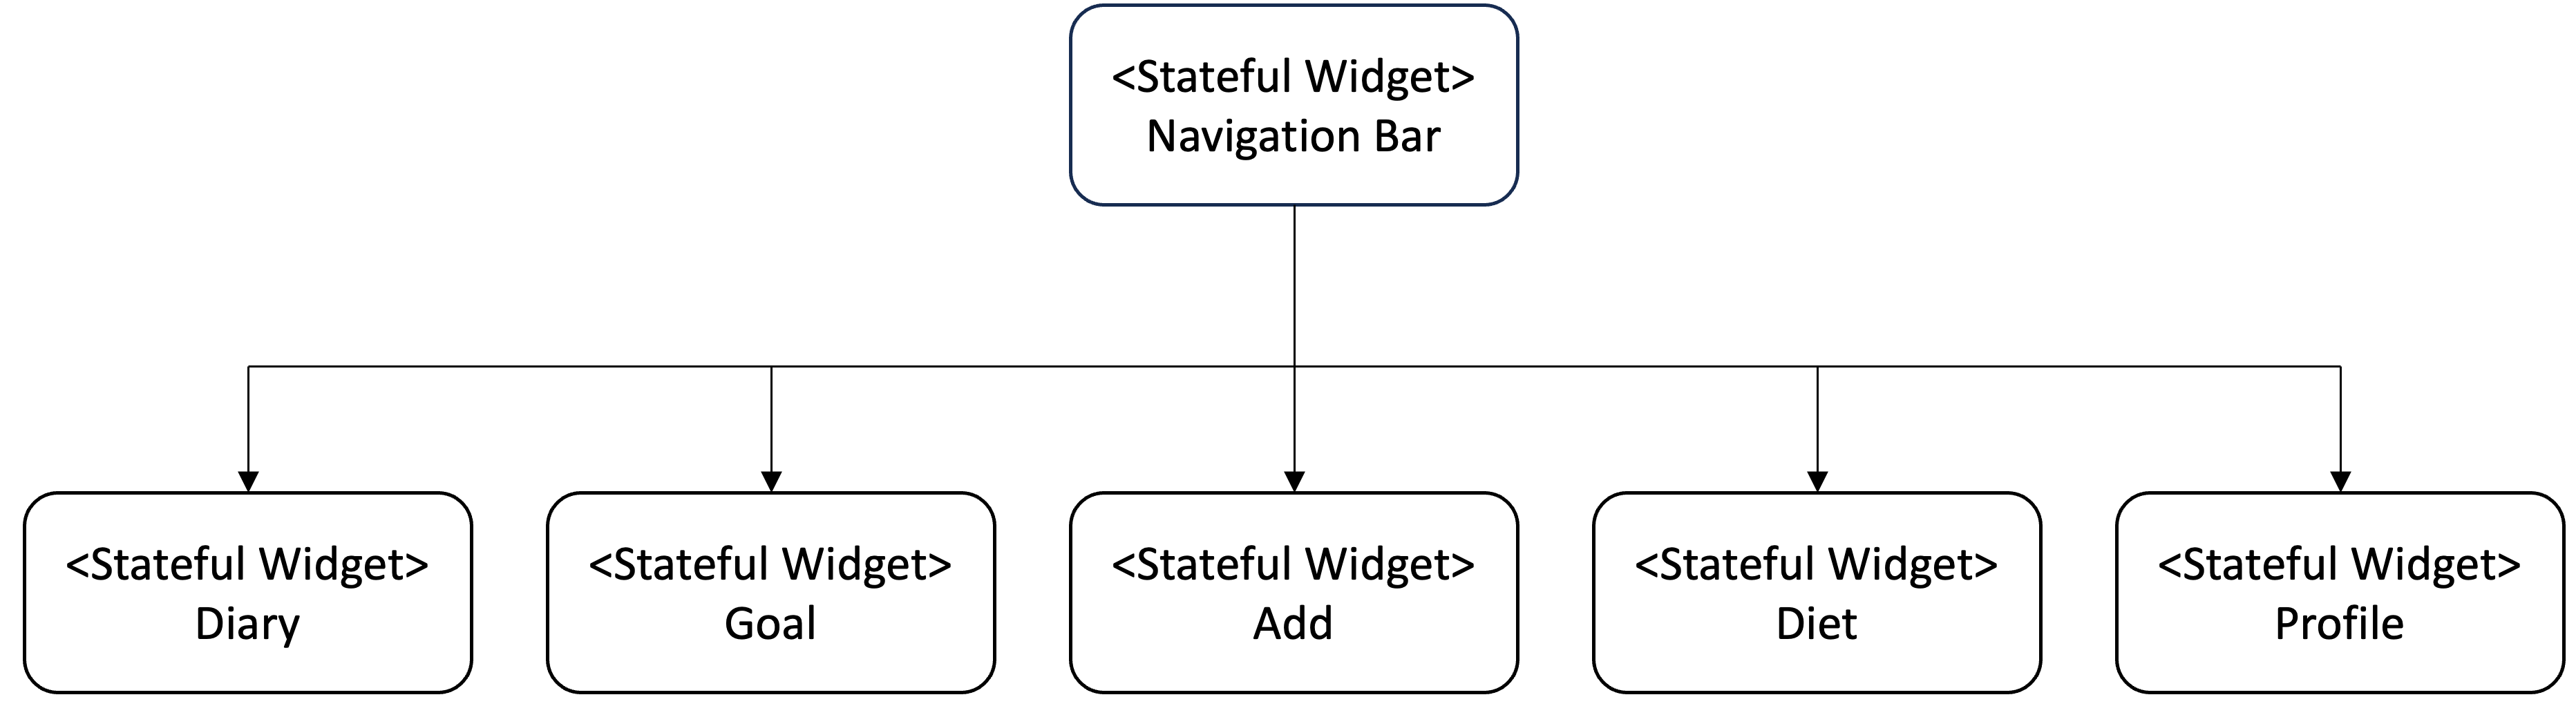
\includegraphics[scale=0.2]{Images/Navigation.png}
  \caption{Navigation from the Bottom Bar}
\end{figure}

%\subsection{Diary}
%\subsection{Goal}
%\subsection{Diet}
%\subsection{Profile}

% WIDGETS

\section{Barcode Scanner}
A fundamental feature of MacroTracker is the ability to log commercial products quickly. This is achieved by scanning the product's barcode. The barcode number is then used as input with the OpenFoodFacts APIs described above, and the product's information is retrieved from the database. 
The plugin used by the app is \textbf{Flutter Barcode Scanner} - \url{https://github.com/FlutterFlow/flutter_barcode_scanner}.
The plugin provides the logic code and the UI for the scan. 
The device's camera is activated and the user is guided to frame the barcode in the space. 
Upon a scan, the app registers the barcode and converts the numbers to a string.
The scan works in different orientations and is flexible, so that the scan is seamless and easy to achieve. 

\section{Apple Health}
The application has been developed from the start with Apple's Health ecosystem in mind.
Apple Health is a comprehensive health and fitness platform developed by Apple Inc. It is an app available on Apple devices, such as iPhones and Apple Watches, and is designed to help individuals monitor and manage various aspects of their health and well-being.
Apple Health serves as a centralized hub for collecting and organizing health-related data from various sources, including built-in sensors, third-party fitness trackers, and compatible health and wellness apps. The app can track a wide range of health metrics, such as daily steps, distance walked or run, heart rate, sleep patterns, calories burned, and more.
In addition to tracking physical activity, Apple Health allows users to input and monitor other health data manually, such as weight, body measurements, and \textit{dietary intake}. This enables users to have a holistic view of their health and fitness progress over time.
MacroTracker seamlessly integrates with Apple Health, ensuring that the data captured by the app is automatically saved and contributes to the user's overall health profile. By storing this information in Apple Health, MacroTracker empowers users to gain a comprehensive understanding of their health, enabling them to analyze their macronutrient intake alongside other vital health metrics. This holistic approach enables individuals to make informed decisions about their diet, identify areas for improvement, and strive for a balanced and nourishing lifestyle.
To achieve this, the apps uses the plugin \textbf{Health} - \url{https://pub.dev/packages/health} - a wrapper for HealthKit that:
\begin{itemize}
    \item Handles the permissions to access health data.
    \item Writes health data to Apple Health's data store. 
\end{itemize}

When a food is logged by the user, MacroTracker automatically writes to Health the calorie intake and the macronutrients intake. Obviously, a removal or a modification of an insertion is reflected in Health. 

\section{Notifications}
The app provides the user the ability to receive a daily notification that reminds them to log their diet. The notification is useful to help developing healthy habits by keeping up to date the food intake, to let the athlete observe their progress. 
The notification has been thought out to not be intrusive, so the user will receive the daily notification only if they actively use the app. It empowers individuals to establish a consistent routine for logging their diet without feeling overwhelmed or burdened by intrusive alerts.
The app's non-intrusive daily notification feature plays a vital role in assisting users to develop healthy habits, maintain consistency in tracking their diet, and stay motivated towards their dietary goals.
The app uses the \textbf{Flutter Local Notifications} plugin - \url{https://pub.dev/packages/flutter_local_notifications} - to schedule and deliver the notification to the user. 
A local approach has been chosen, as there is no need for the backend to deliver this notification as it is static. 
The notification's component is called \texttt{Local Notification Service}, and the code is executed while using the app, scheduling a notification at the next evening (19:00). This hour has been chosen as it is close to dinner and should not interfere with social events. 

\chapter{Dependencies}
\section{Plugins}
The table provided below enumerates the noteworthy plugins that have been incorporated into the application as dependencies. Each plugin is accompanied by a rationale for its inclusion, outlining the purpose and justification behind its integration.

\begin{table} [H]
\centering
\begin{tabular}{|p{5cm}|p{10cm}|}
\hline
\textbf{Plugin} & \textbf{Use} \\[0.5ex]
\hline
\textit{Cloud Firestore} & Necessary for the usage of Cloud Firestore API. \\[0.5ex]
\hline
\textit{Firebase Auth} & Necessary for the handling of the user's credentials, login and sign up. \\[0.5ex]
\hline
\textit{Flutter Local Notifications} & Allows to receive a daily notification to remind the user to log their data. \\[0.5ex]
\hline
\textit{Open Food Facts} & APIs that handle the search of a commercial product through its barcode. Retrieves the product's information. \\[0.5ex]
\hline
\textit{Health} & Allows MacroTracker to interact with Apple Health's HealthKit. Used to save dietary intake to Health's datastore. \\[0.5ex]
\hline
\end{tabular}
\caption{Most significant plugins used and related description.}
\end{table}

\chapter{User Interface}
\section{Design of the app}
The design of the mobile and tablet application has been realized with the help of FlutterFlow platform, in order to create the pages and choosing light mode and dark mode palette colours.
\section{Mobile version}
In the following sections are shown the screens of the \textbf{mobile} application.
Every page will be shown respectively in dark and light mode.
\subsection{Authentication Pages}

\begin{minipage}{\linewidth}
    These are the two initial pages that are displayed once the user opens the app the first time or if they're not logged in. The app firstly shows to the user the login page, then when clicking on the \emph{Register} button, it displays the other one.
\end{minipage}

\begin{figure}[!ht]
  \centering
  
\includegraphics[scale=0.1]{Images/Screenshots/Mobile/Login.png}
  
\includegraphics[scale=0.1]{Images/Screenshots/Mobile/LoginLight.png}
  \caption{Login page}
\end{figure}

\begin{figure}[!h]
  \centering
  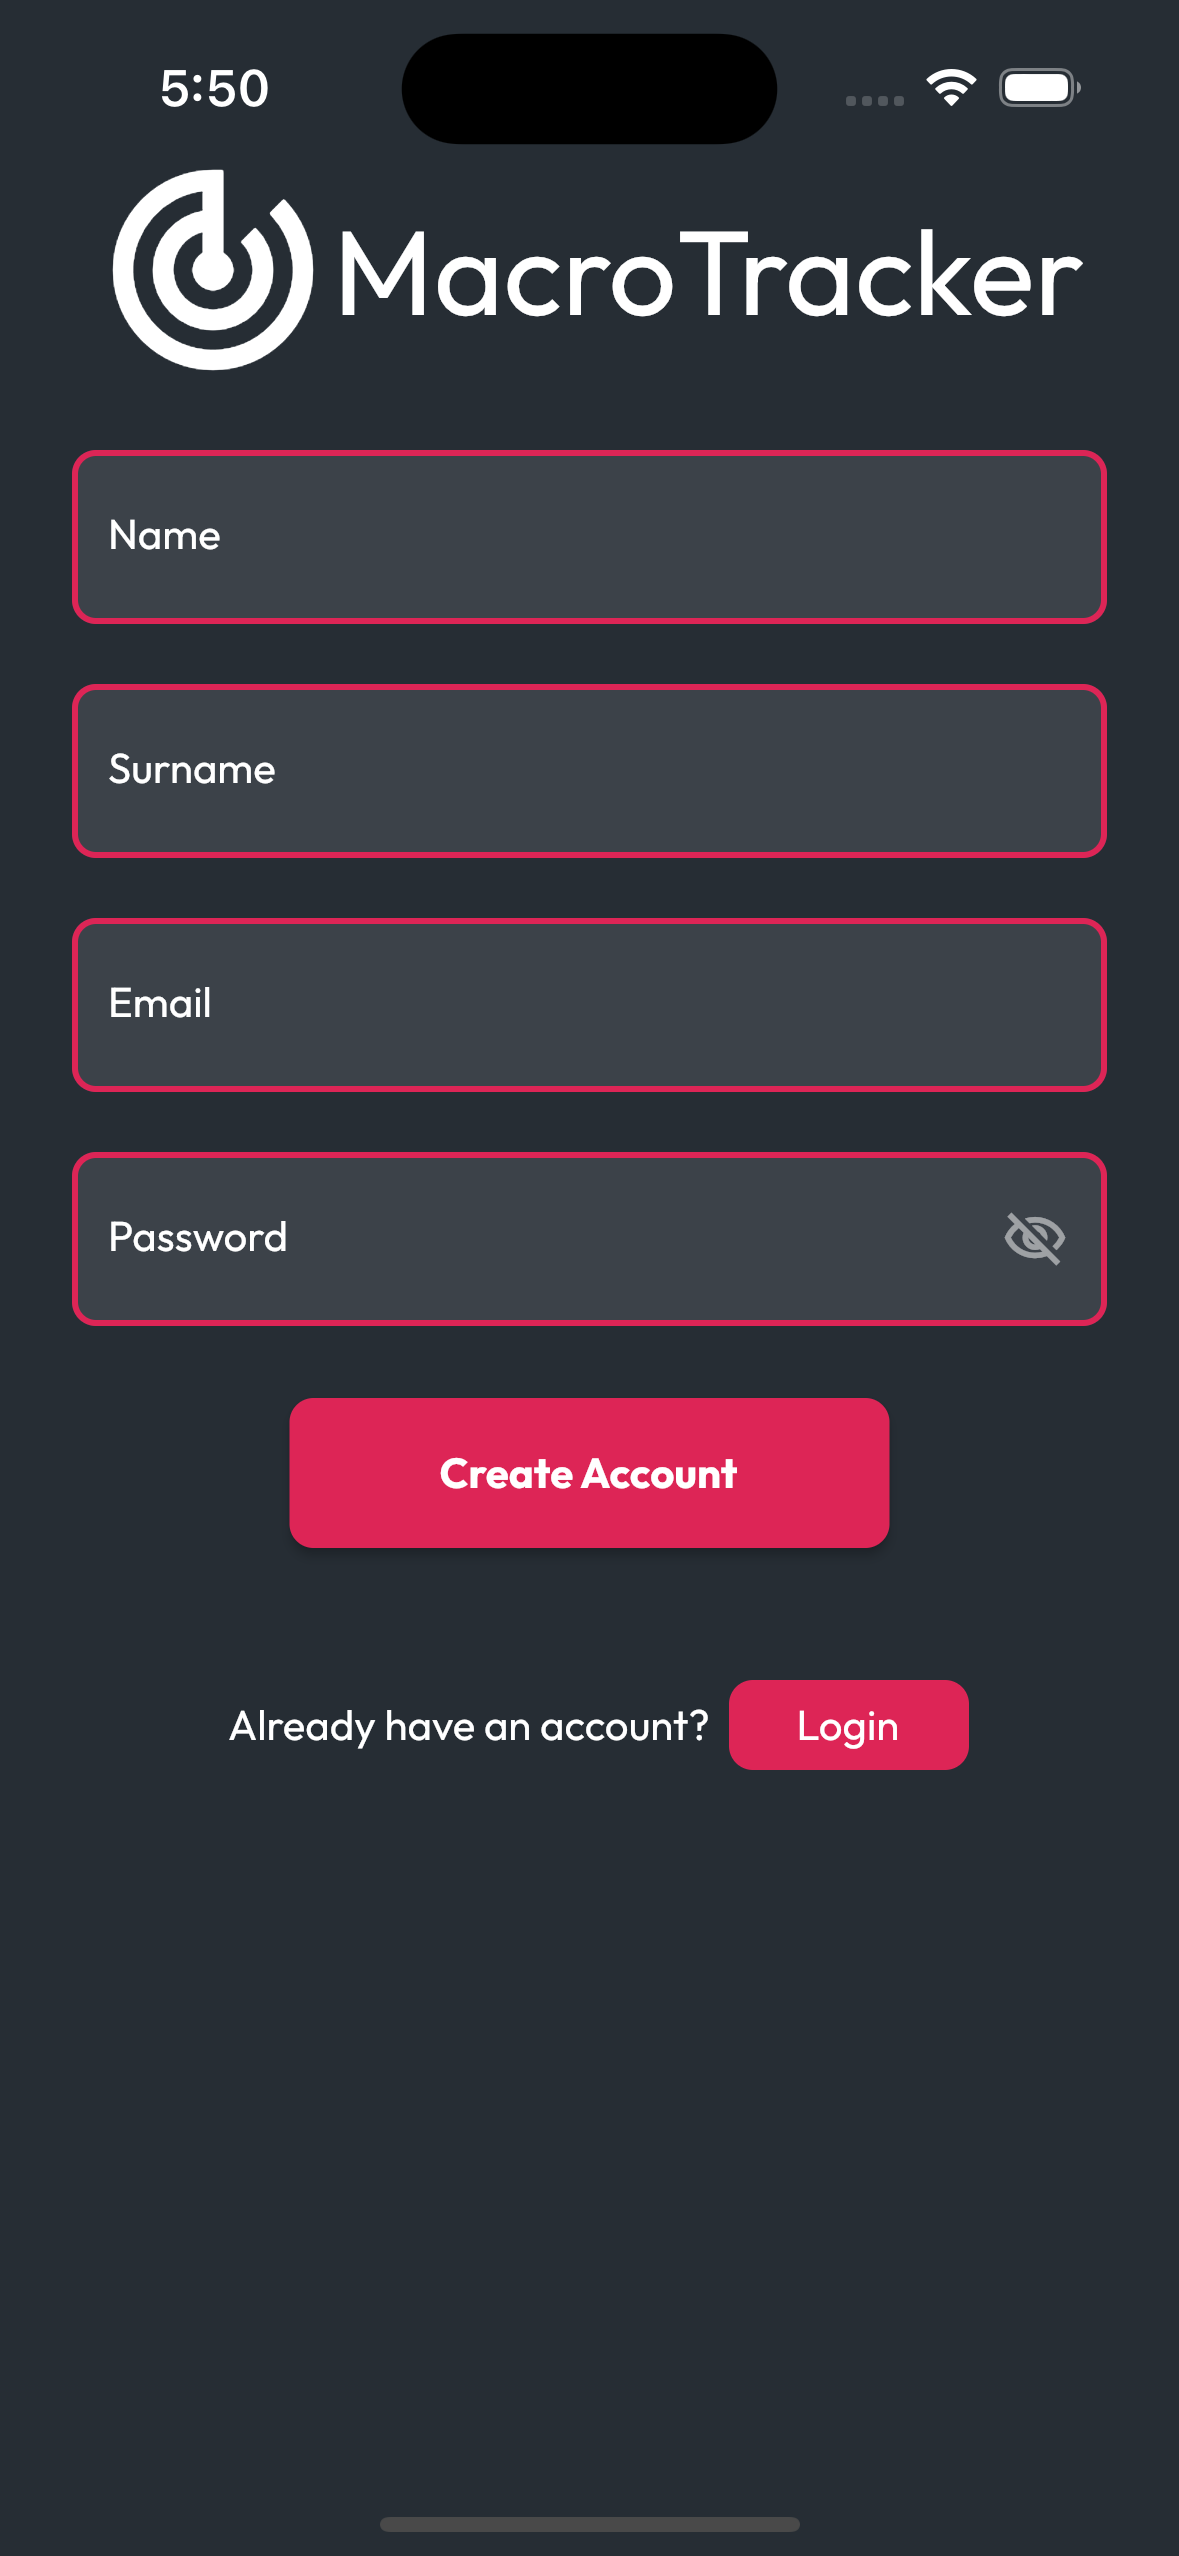
\includegraphics[scale=0.1]{Images/Screenshots/Mobile/Register.png}
  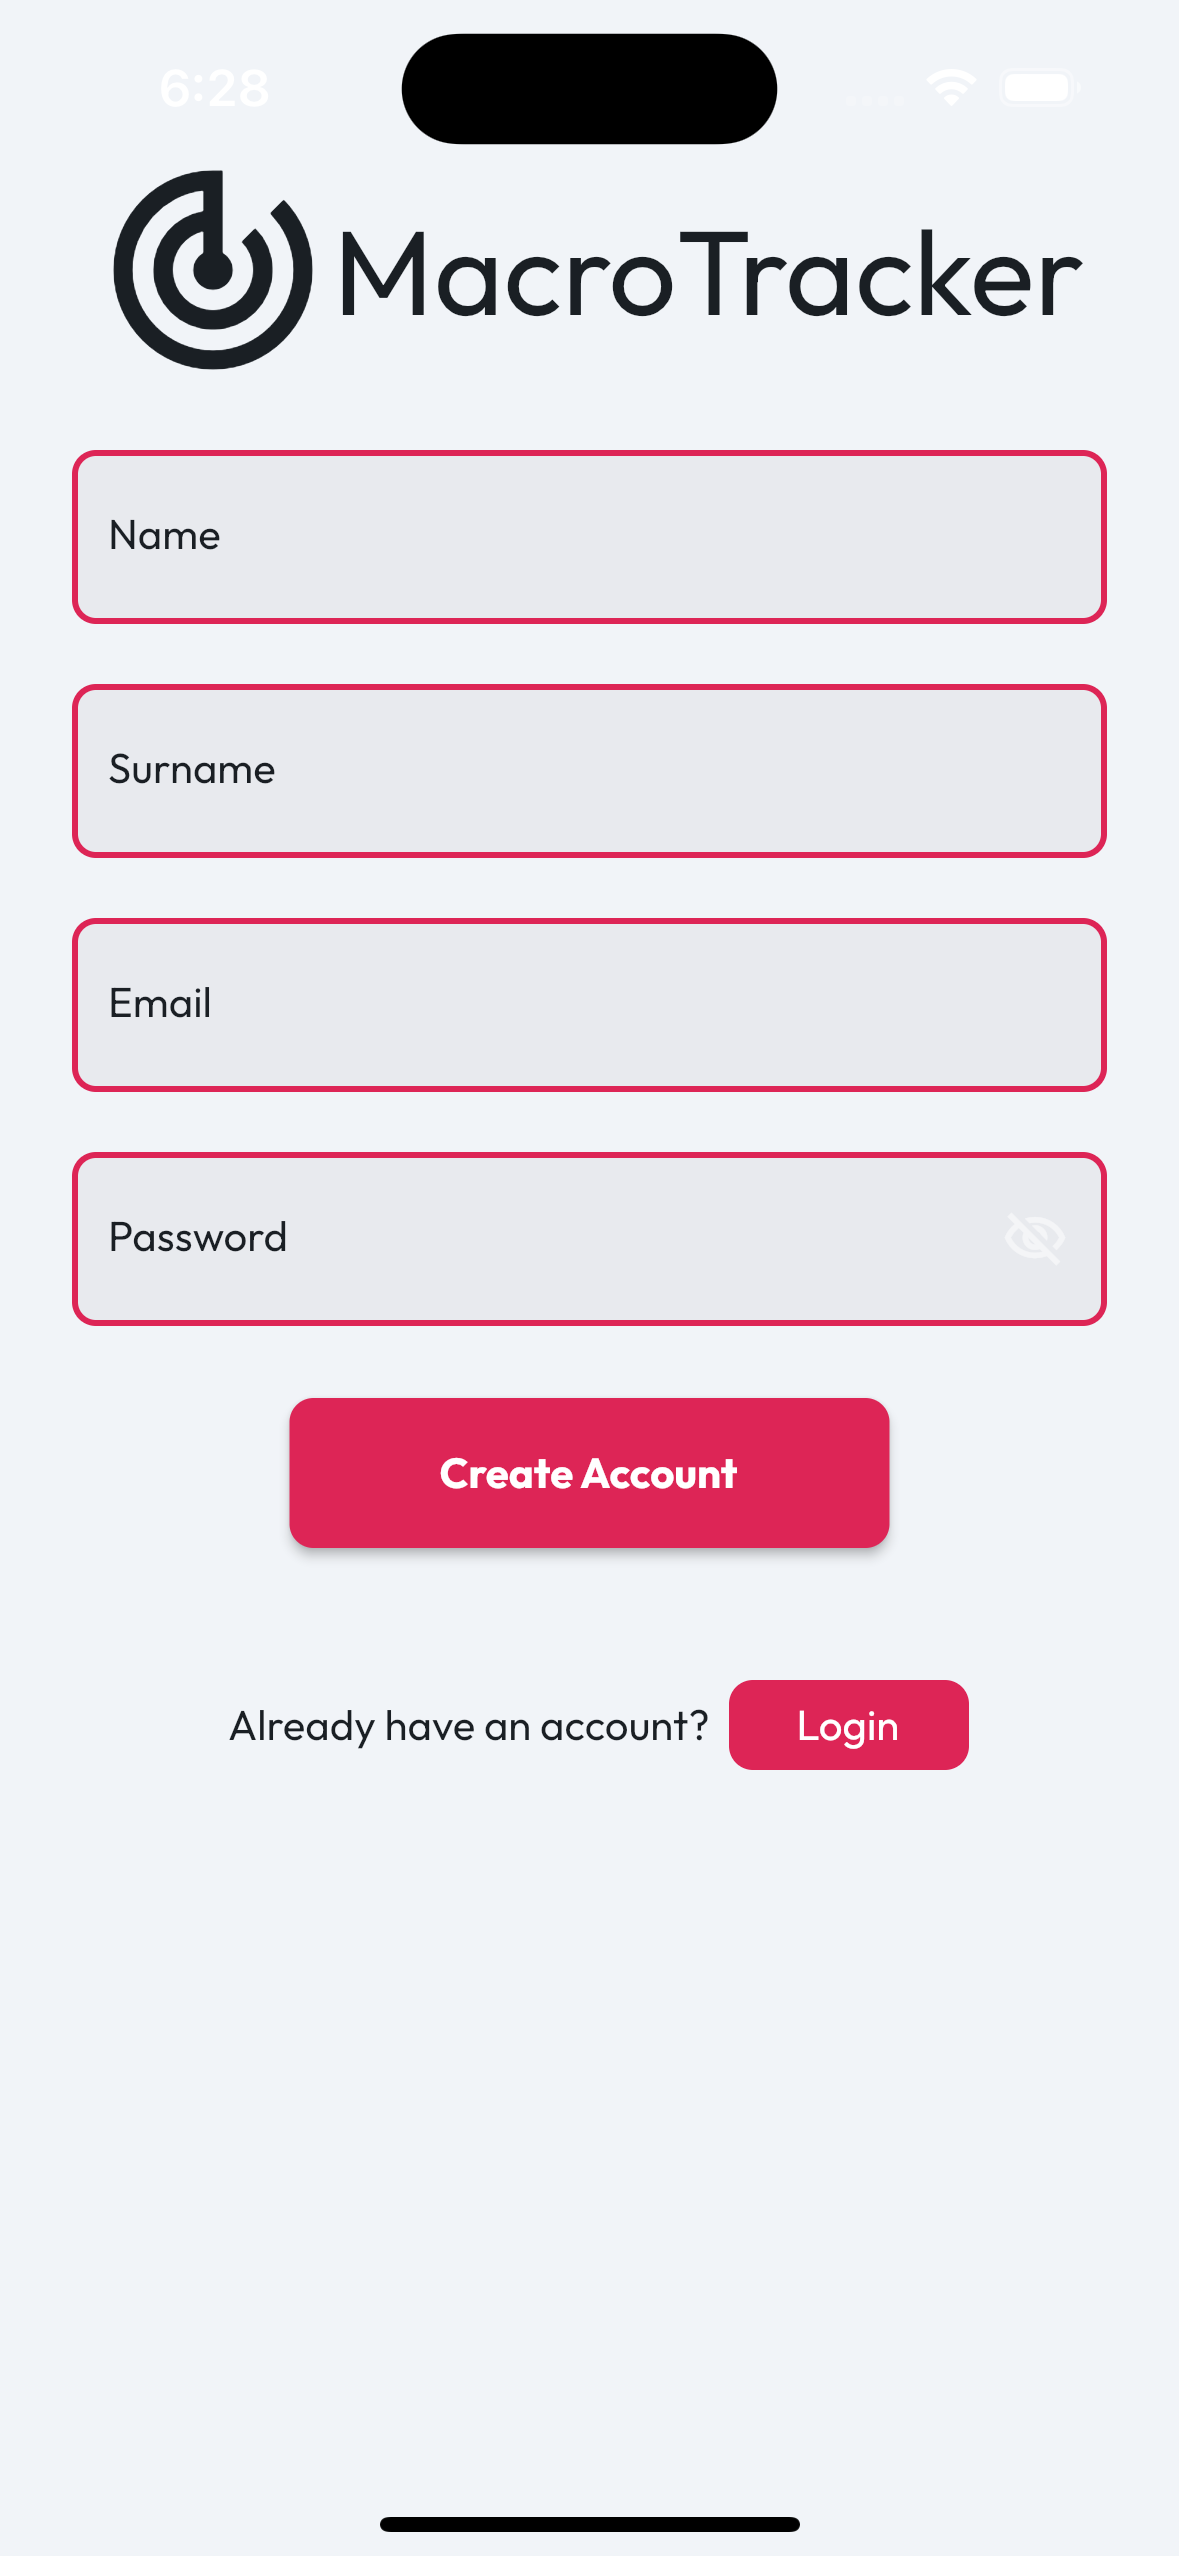
\includegraphics[scale=0.1]{Images/Screenshots/Mobile/RegisterLight.png}
  \caption{Register page}
\end{figure}

\clearpage

\subsection{Diary page}
\begin{minipage}{\linewidth}
    This screen shows the main page of the app where it is displayed the current daily progress of the user diet over the fixed goals. It permits the user to add/remove glasses of water and cups of coffee drank in the day. Then it shows the foods inserted in the selected day.
    The calendar on the top enables the user to see the history of their diet assumptions; by clicking on the previous days the page is updated with the data corresponding to the day selected.
\end{minipage}

\begin{figure}[!h]
    \centering
    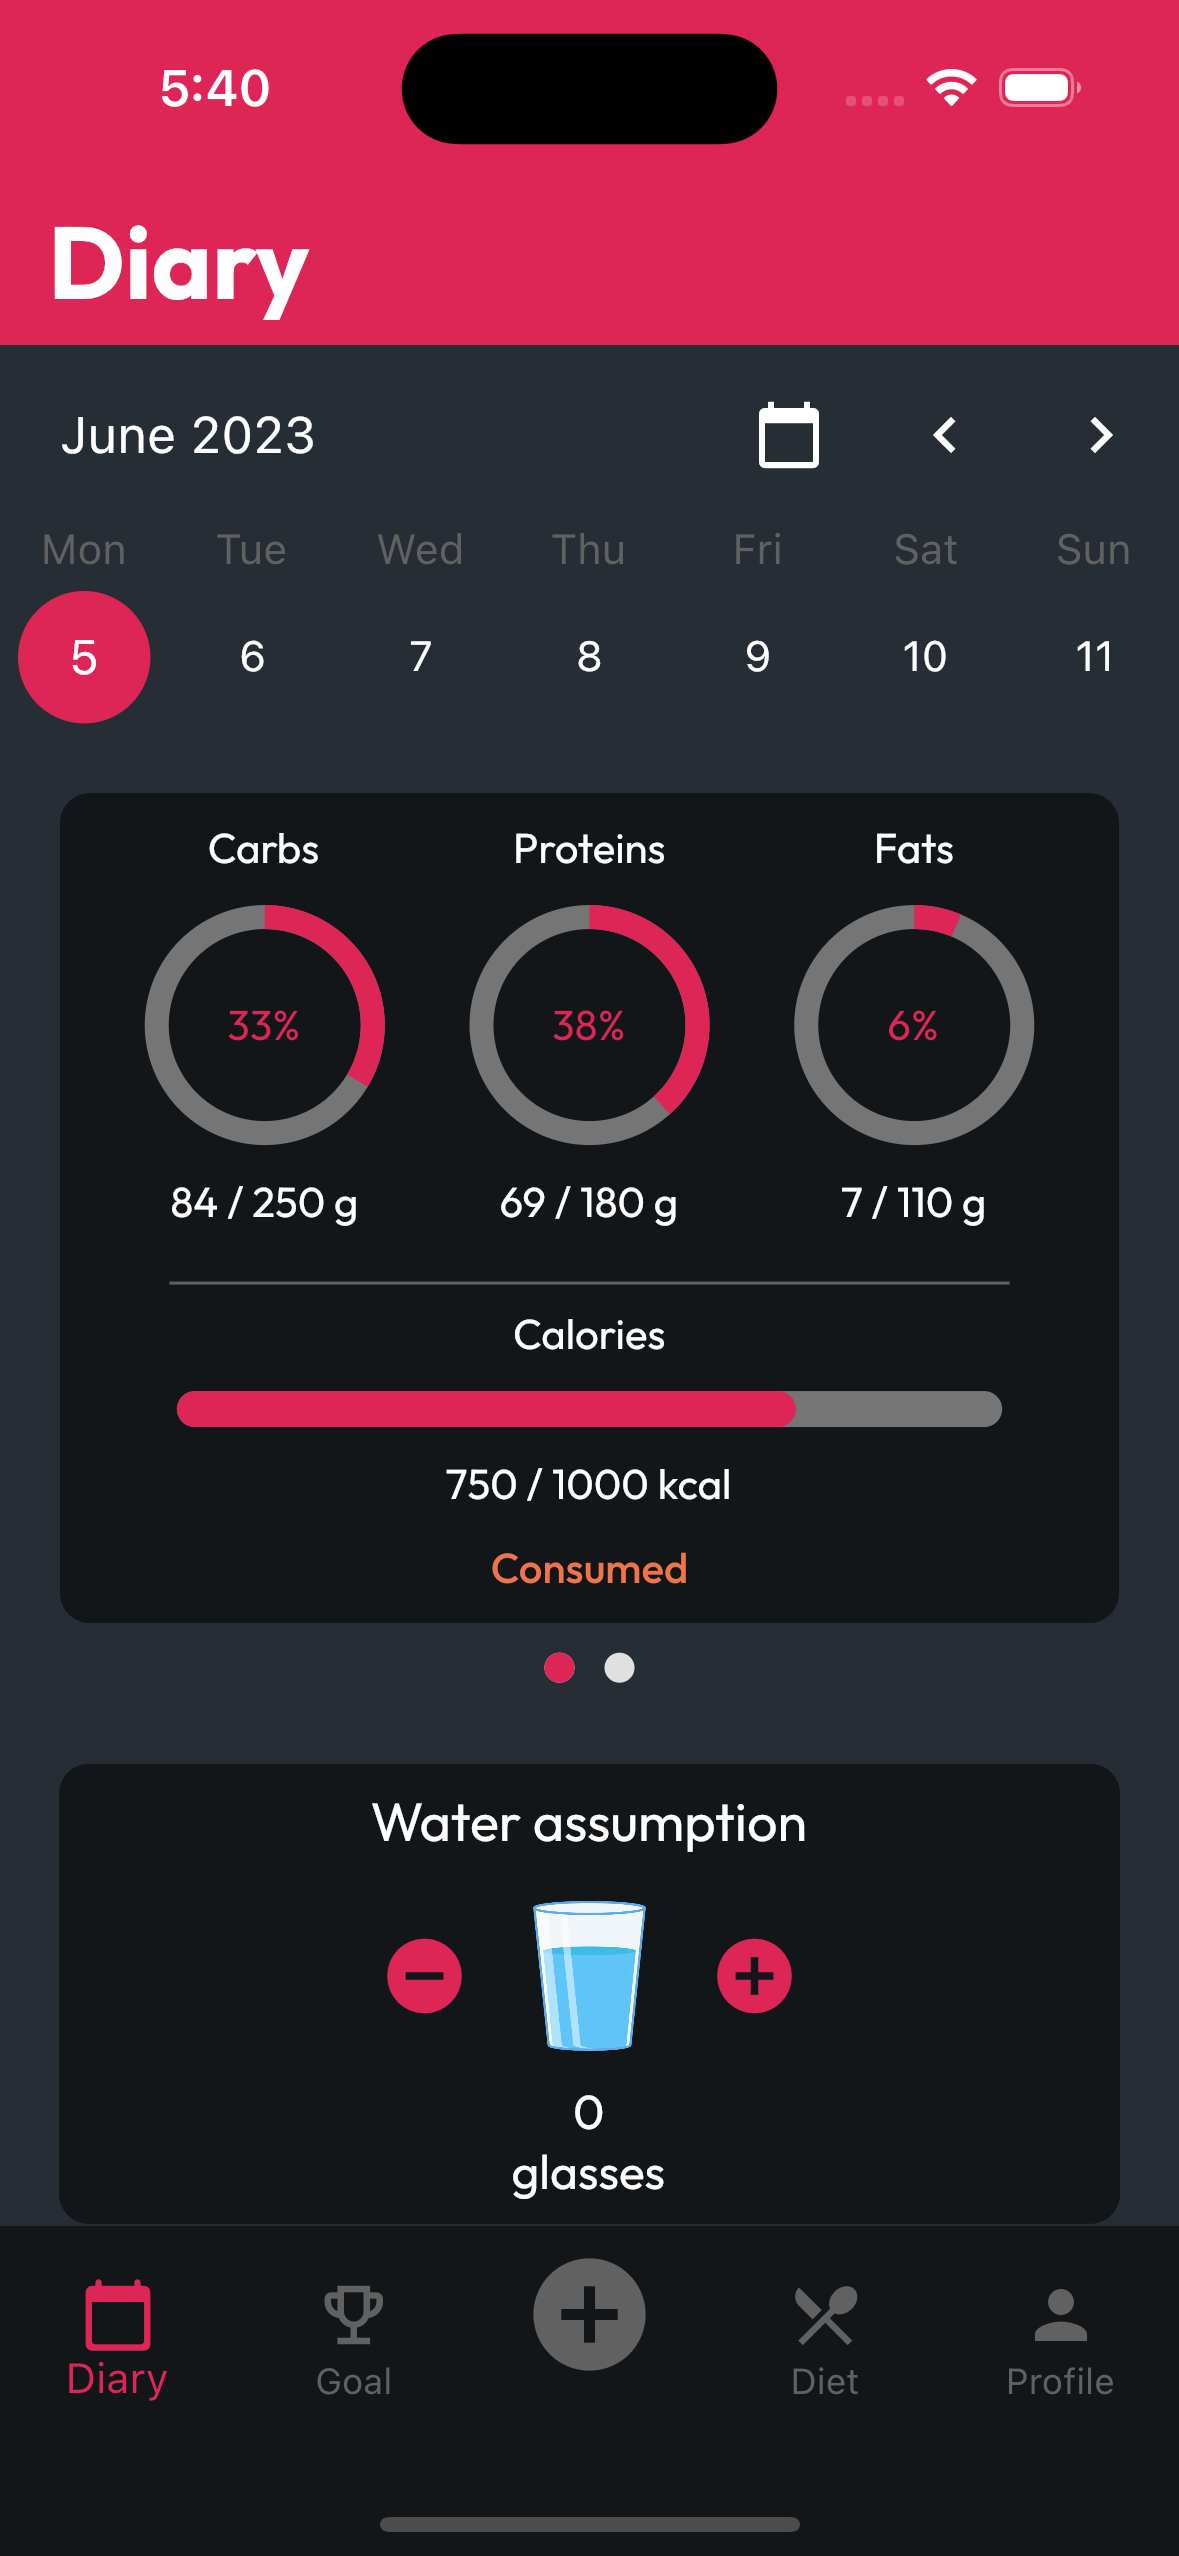
\includegraphics[scale=0.1]{Images/Screenshots/Mobile/Diary1.png}
    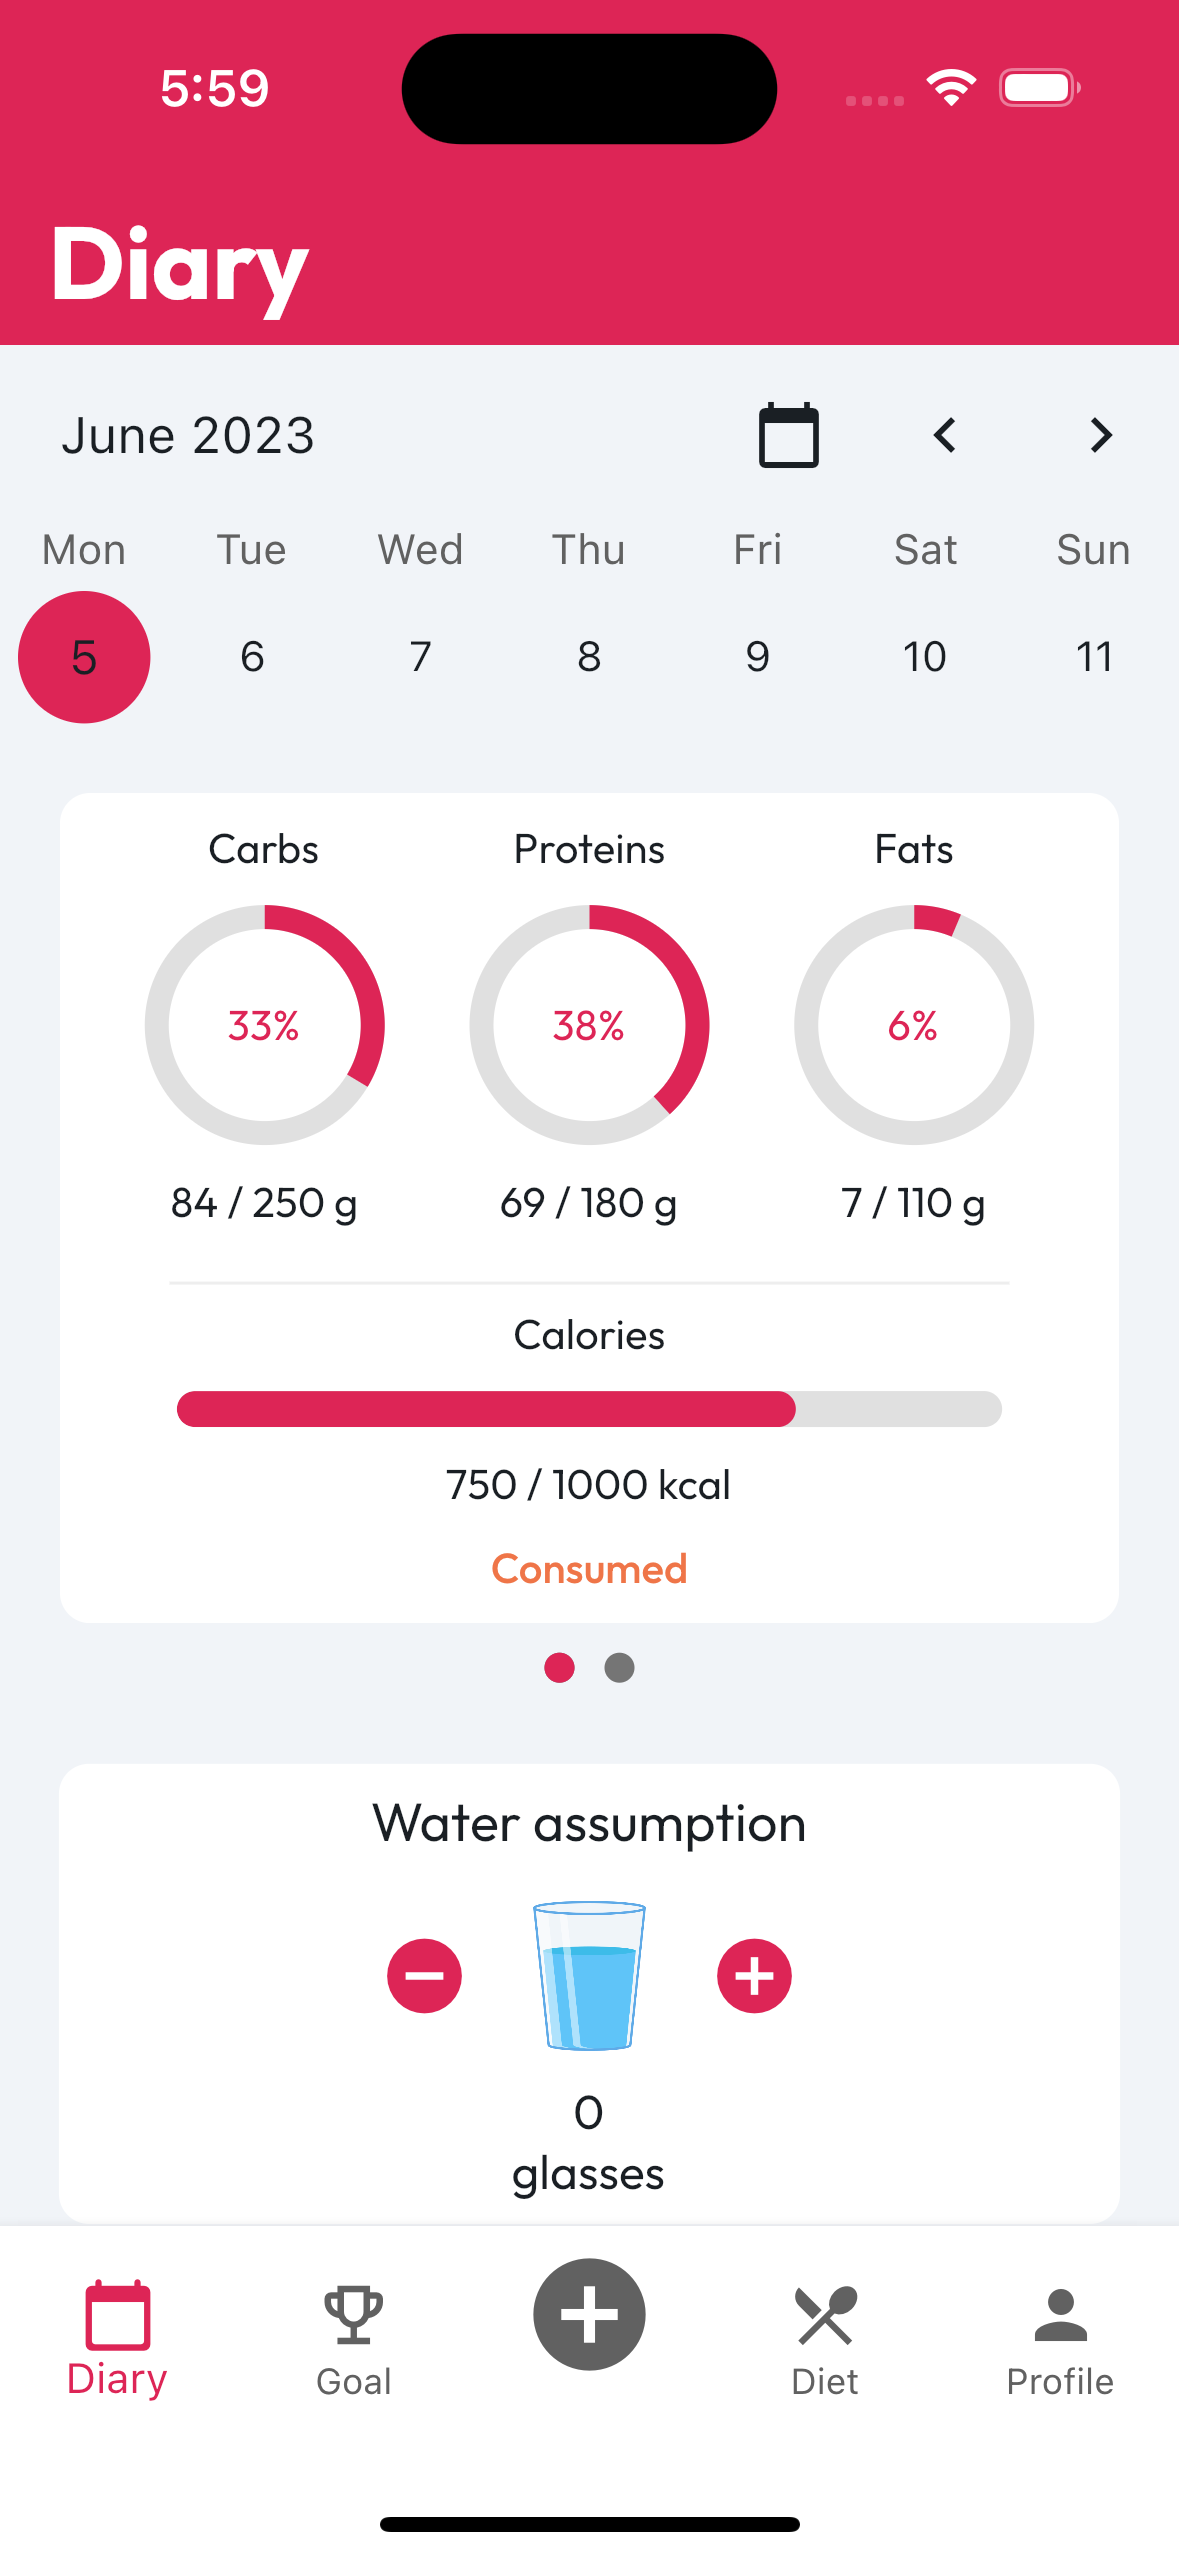
\includegraphics[scale=0.1]{Images/Screenshots/Mobile/Diary1Light.png}
    \caption{Diary page (1 of 2)}
\end{figure}

\begin{figure}[!h]
    \centering
    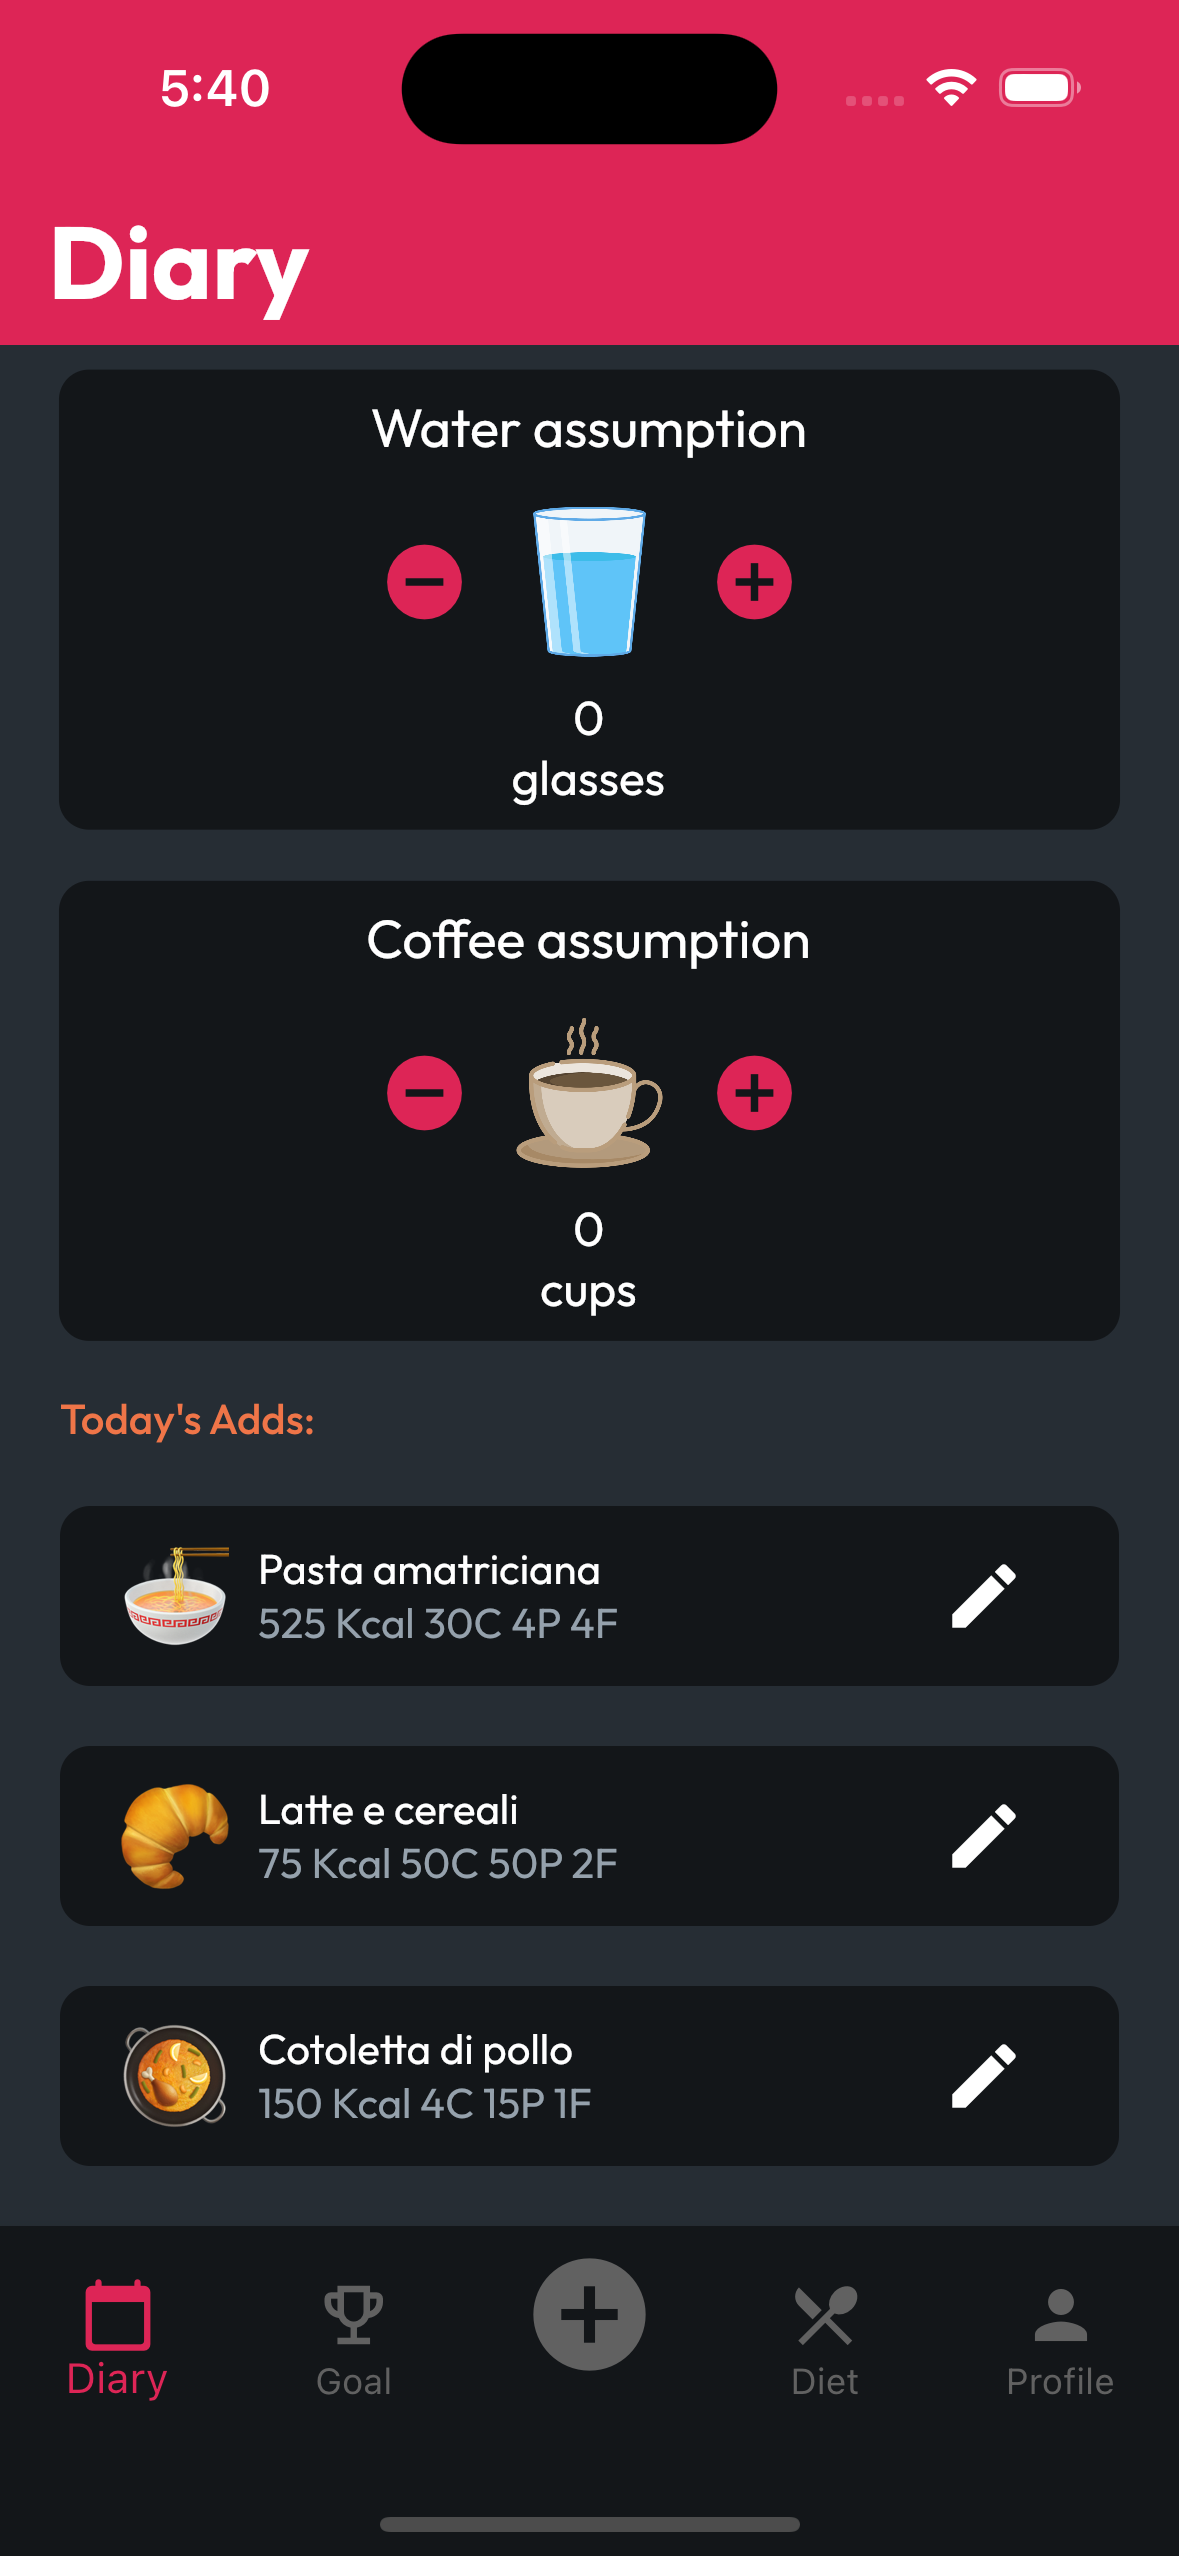
\includegraphics[scale=0.1]{Images/Screenshots/Mobile/Diary2.png}
    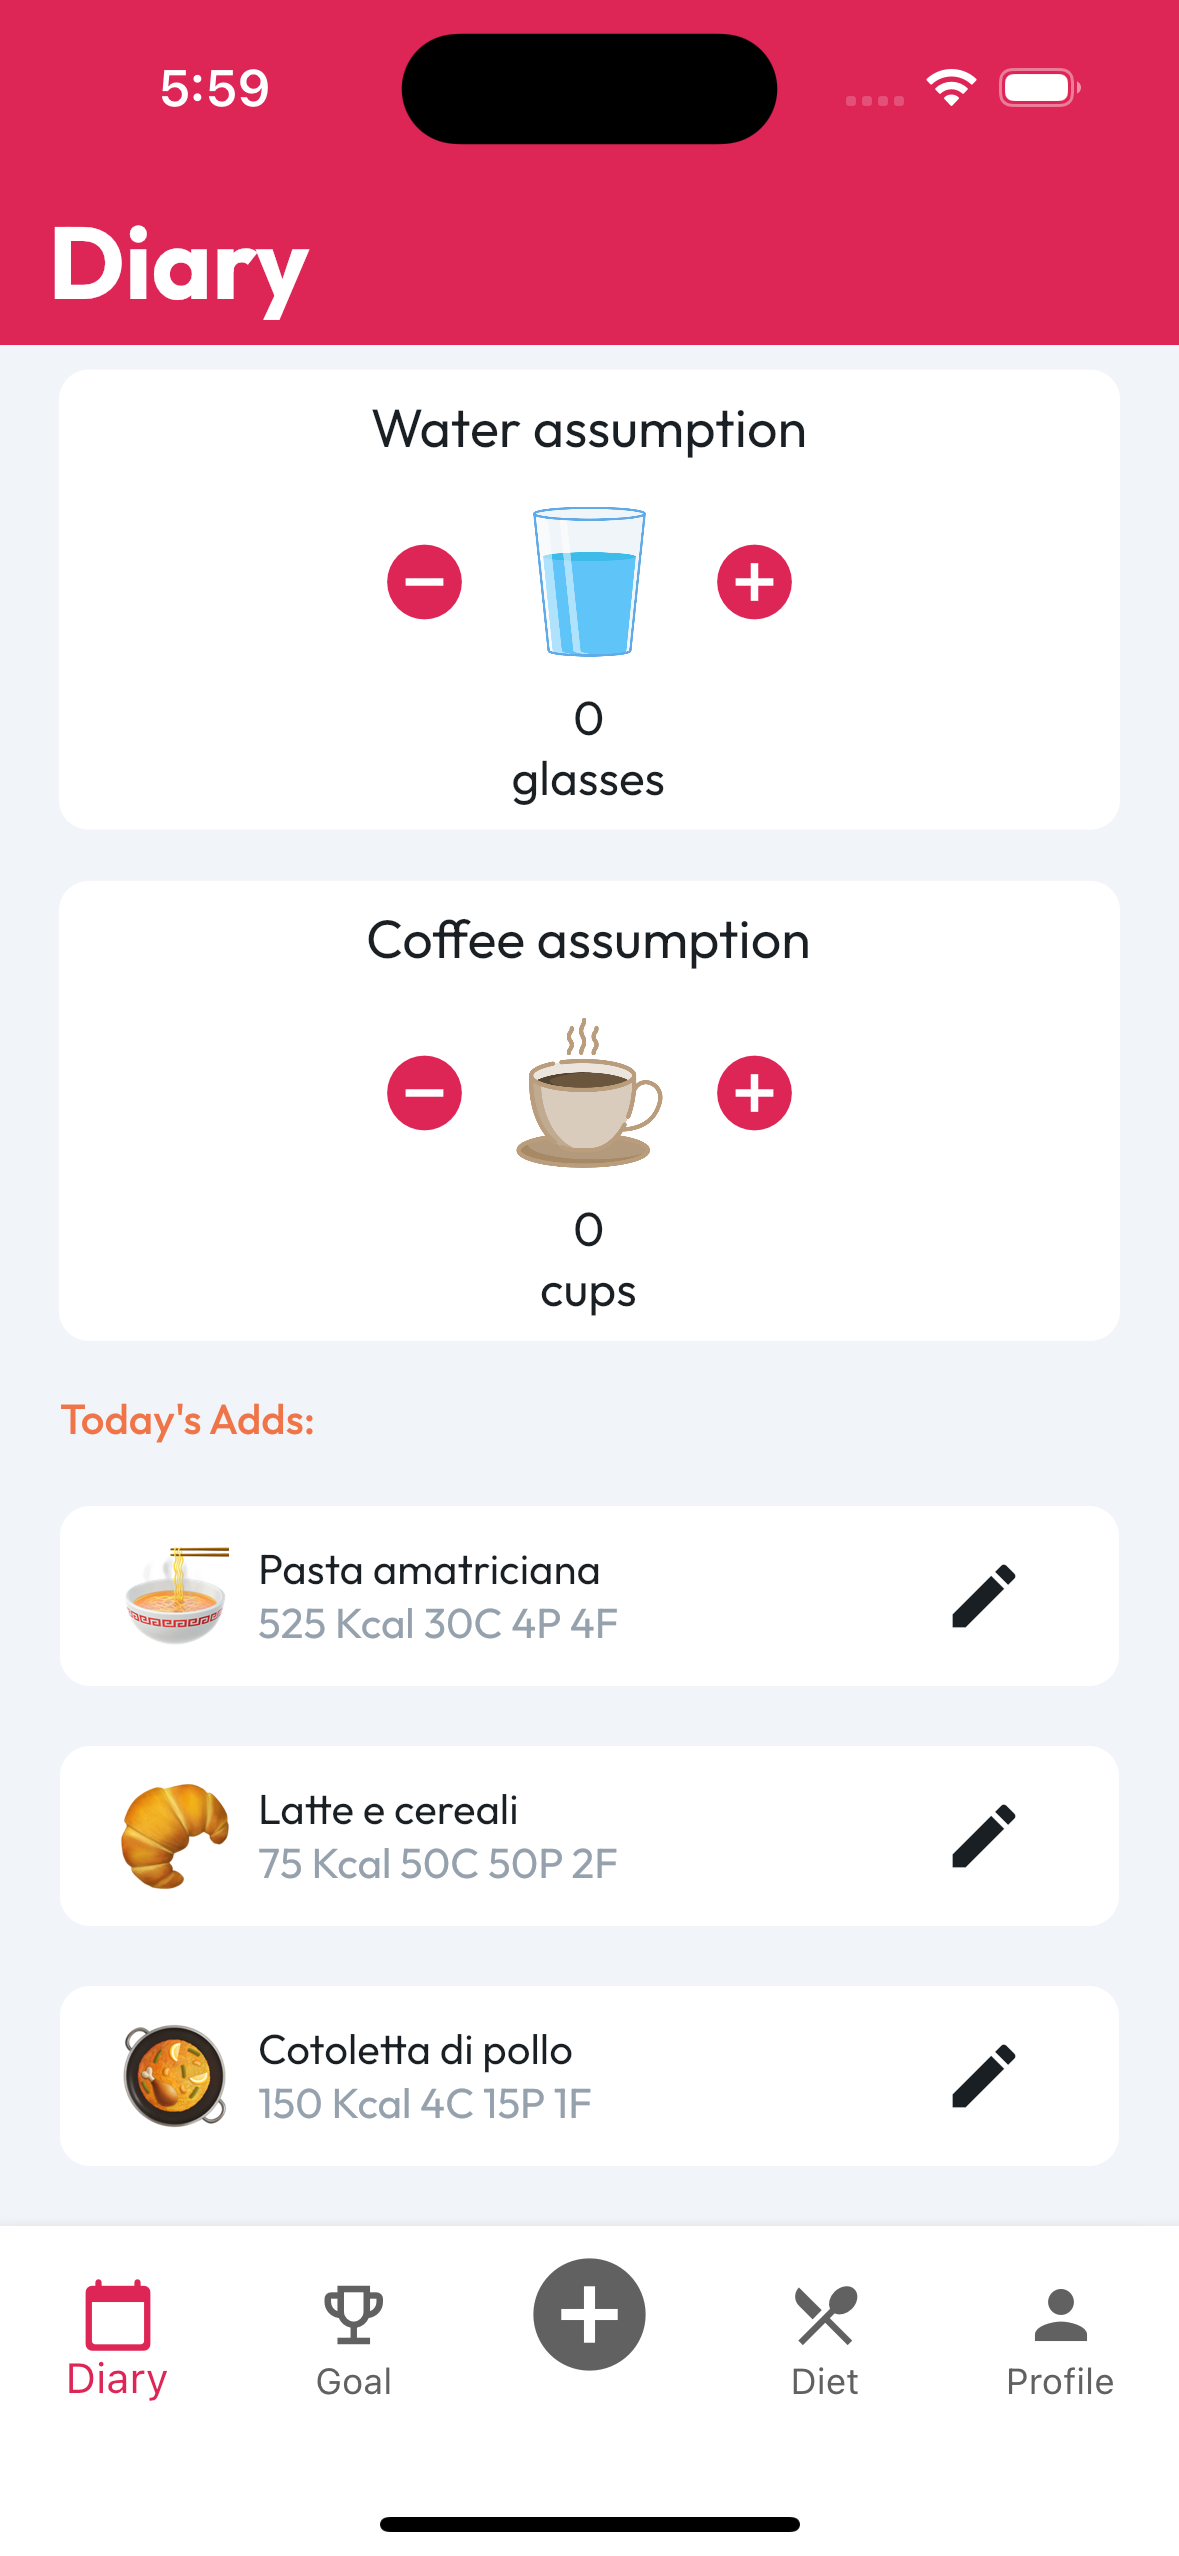
\includegraphics[scale=0.1]{Images/Screenshots/Mobile/Diary2Light.png}
    \caption{Diary page (2 of 2)}
\end{figure}

\begin{figure}[!h]
    \centering
    
\includegraphics[scale=0.7]{Images/Screenshots/Mobile/DiaryFoodItem.png}
    \caption{The single tile of displayed food shows the name of the food, the meal category (icon) and the macro nutrients of the food in a synthetic way.}
\end{figure}

\clearpage

\subsection{Edit food page}

\begin{minipage}{\linewidth}
    This screen is shown when clicking on the \emph{pencil} icon on the single food and permits the user to edit all the food properties or to delete the food clicked.
\end{minipage}

\begin{figure}[!h]
  \centering
  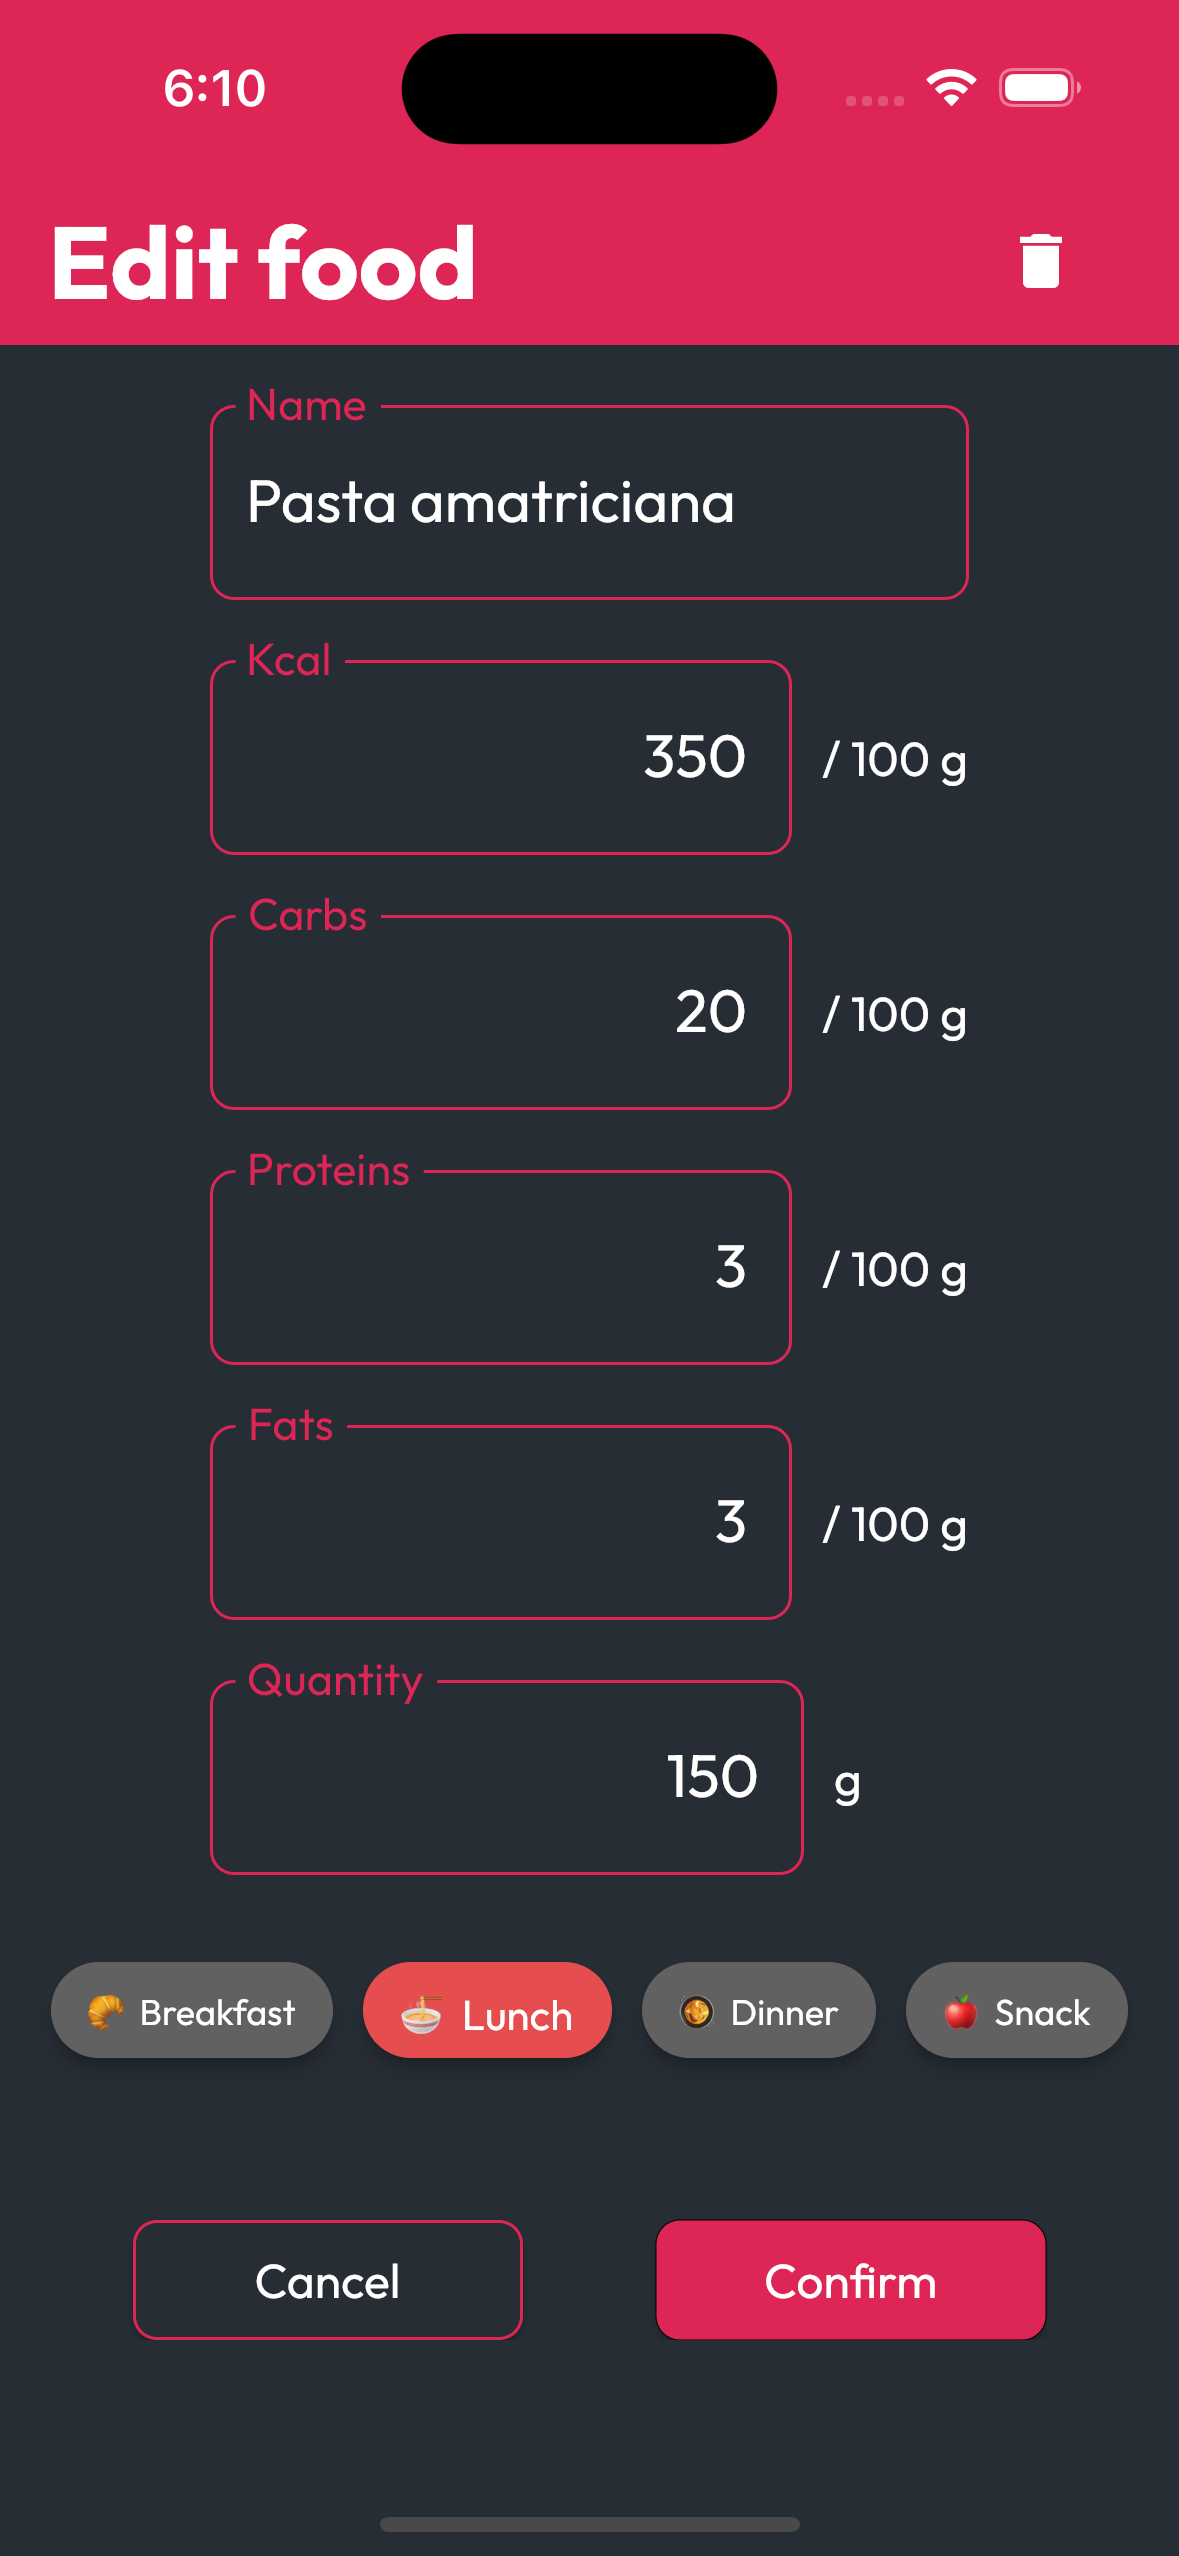
\includegraphics[scale=0.1]{Images/Screenshots/Mobile/EditFood.png}
  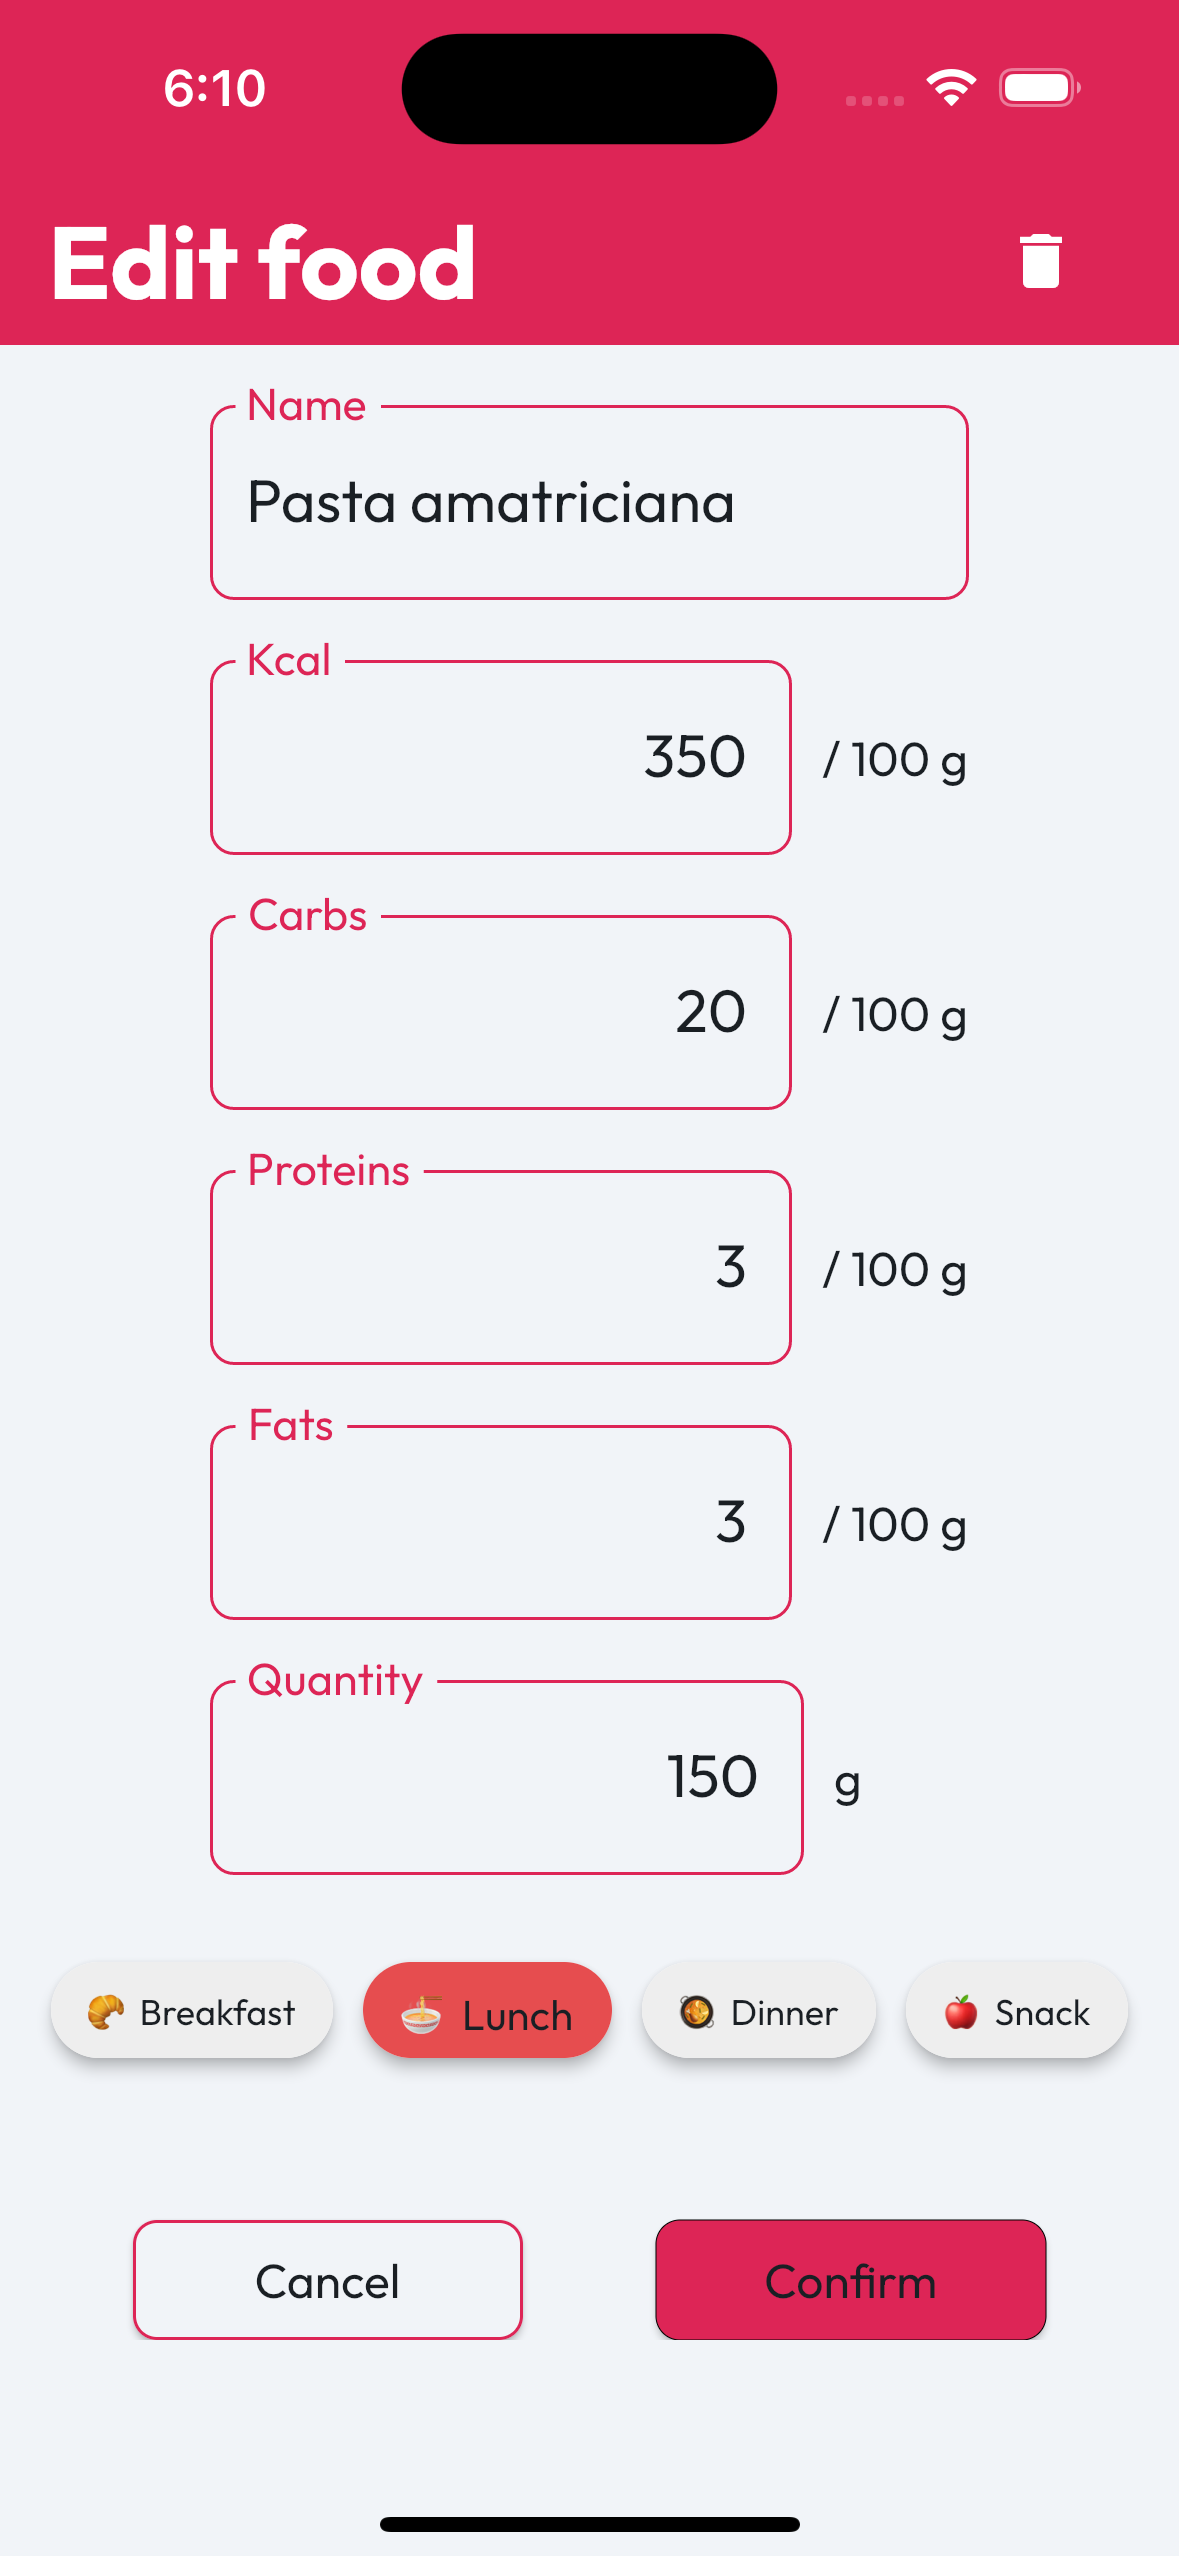
\includegraphics[scale=0.1]{Images/Screenshots/Mobile/EditFoodLight.png}
  \caption{Edit food page}
\end{figure}

\clearpage

\subsection{Goal page}

\begin{minipage}{\linewidth}
    This screen shows the user's fixed goal and permits the user to set them based on their necessities. Below there are some tips related to some typical athlete diet types.
\end{minipage}

\begin{figure}[!h]
  \centering
  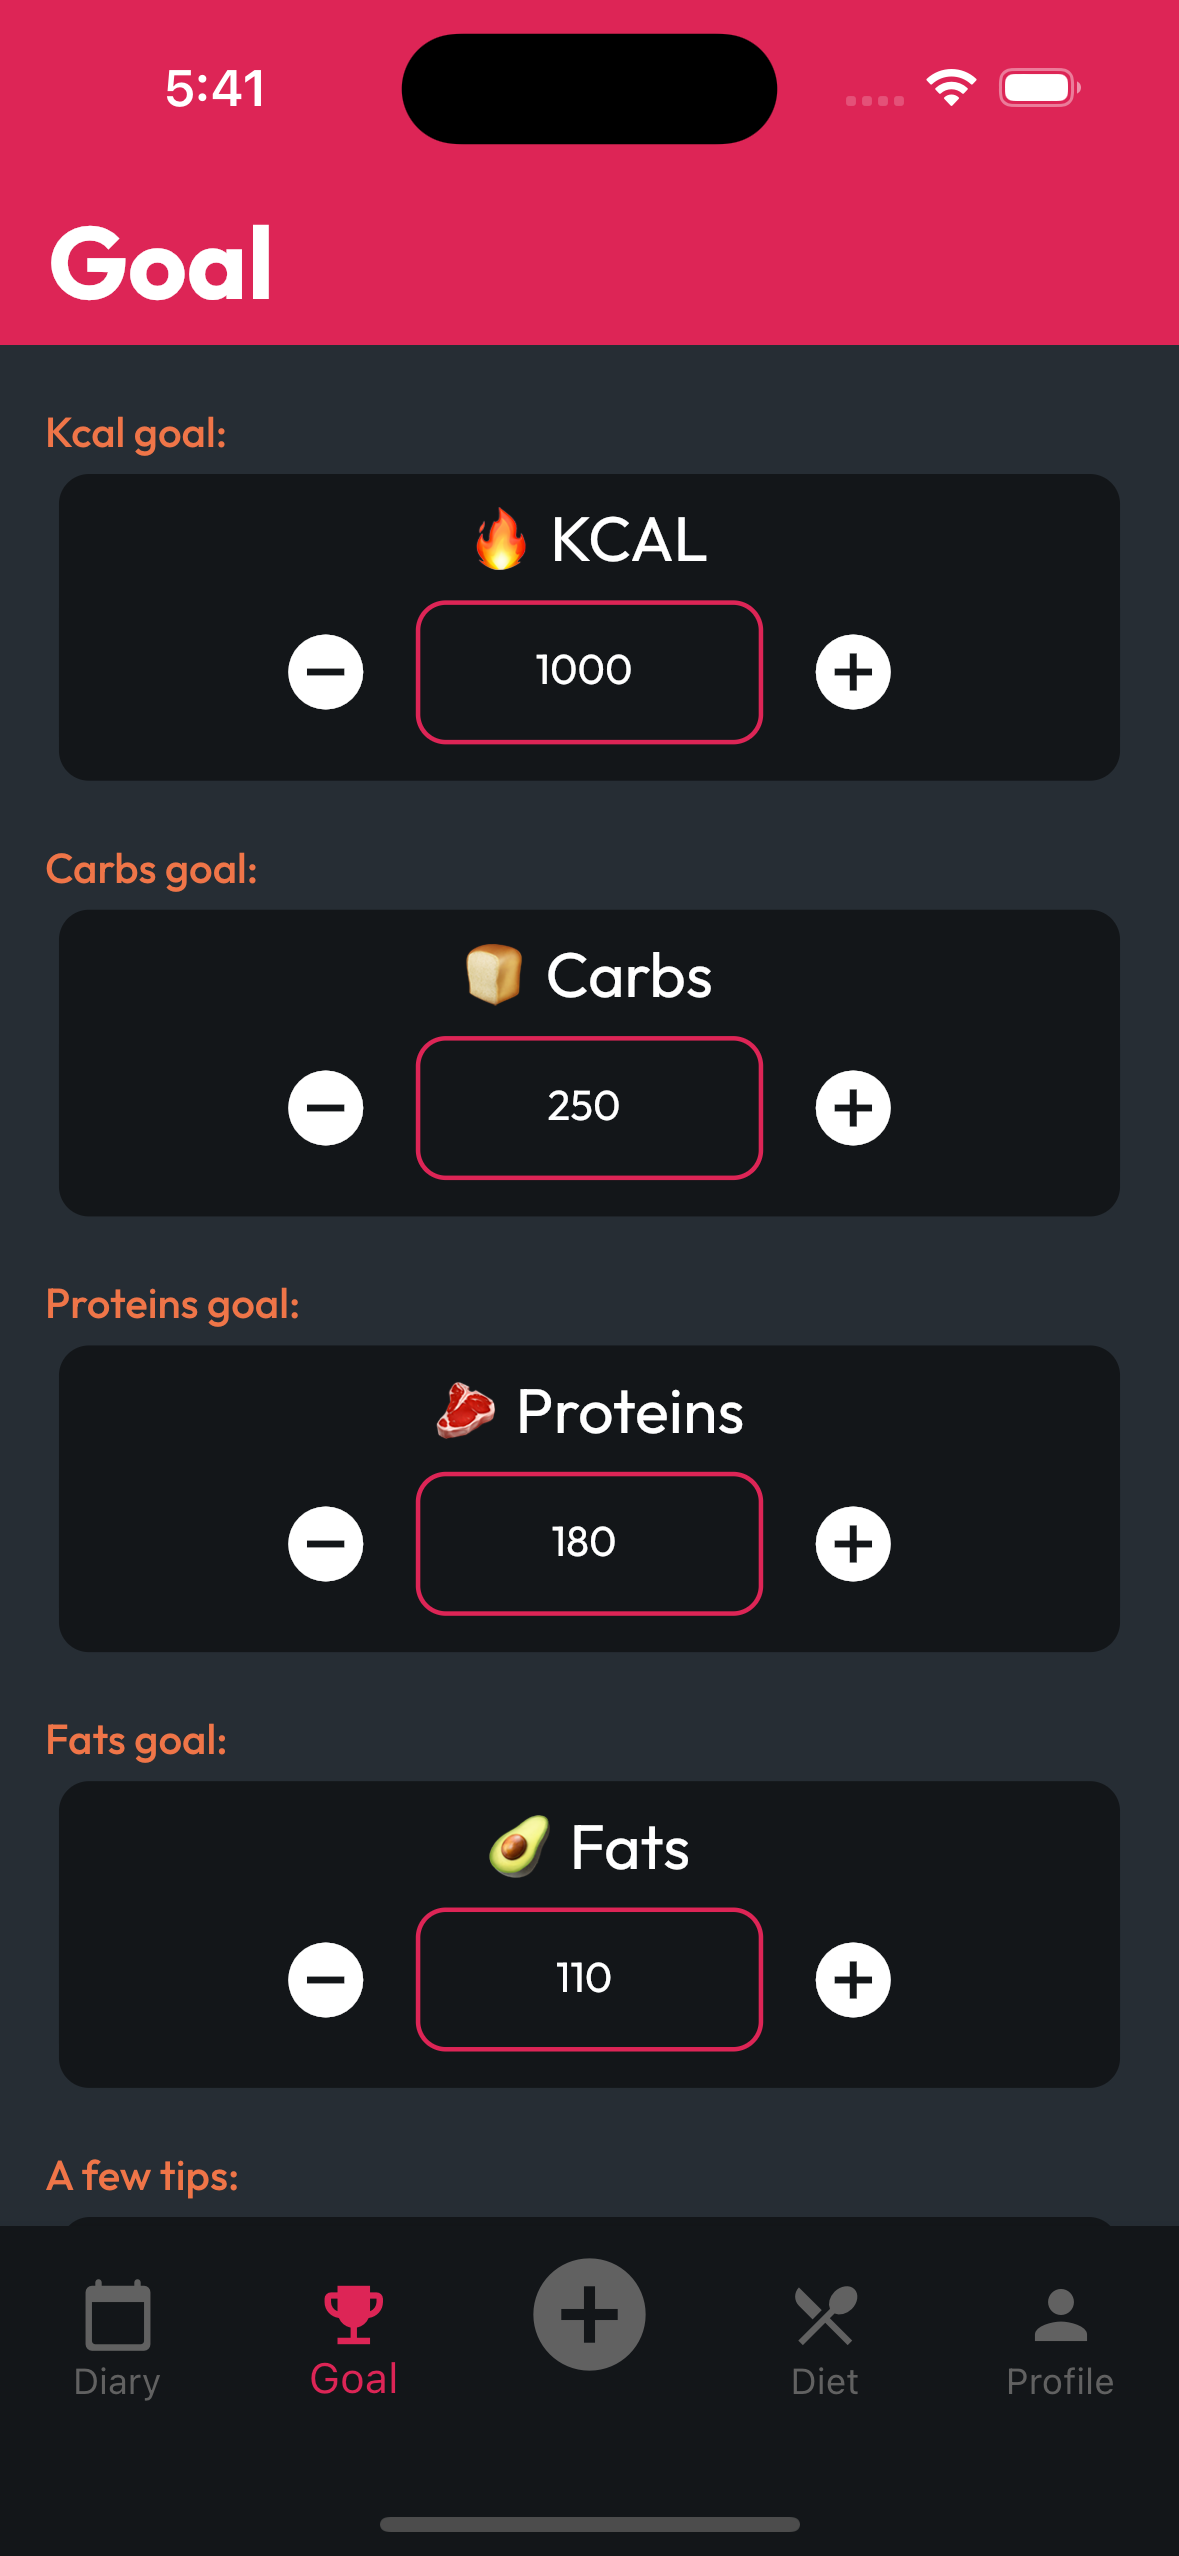
\includegraphics[scale=0.1]{Images/Screenshots/Mobile/Goal1.png}
  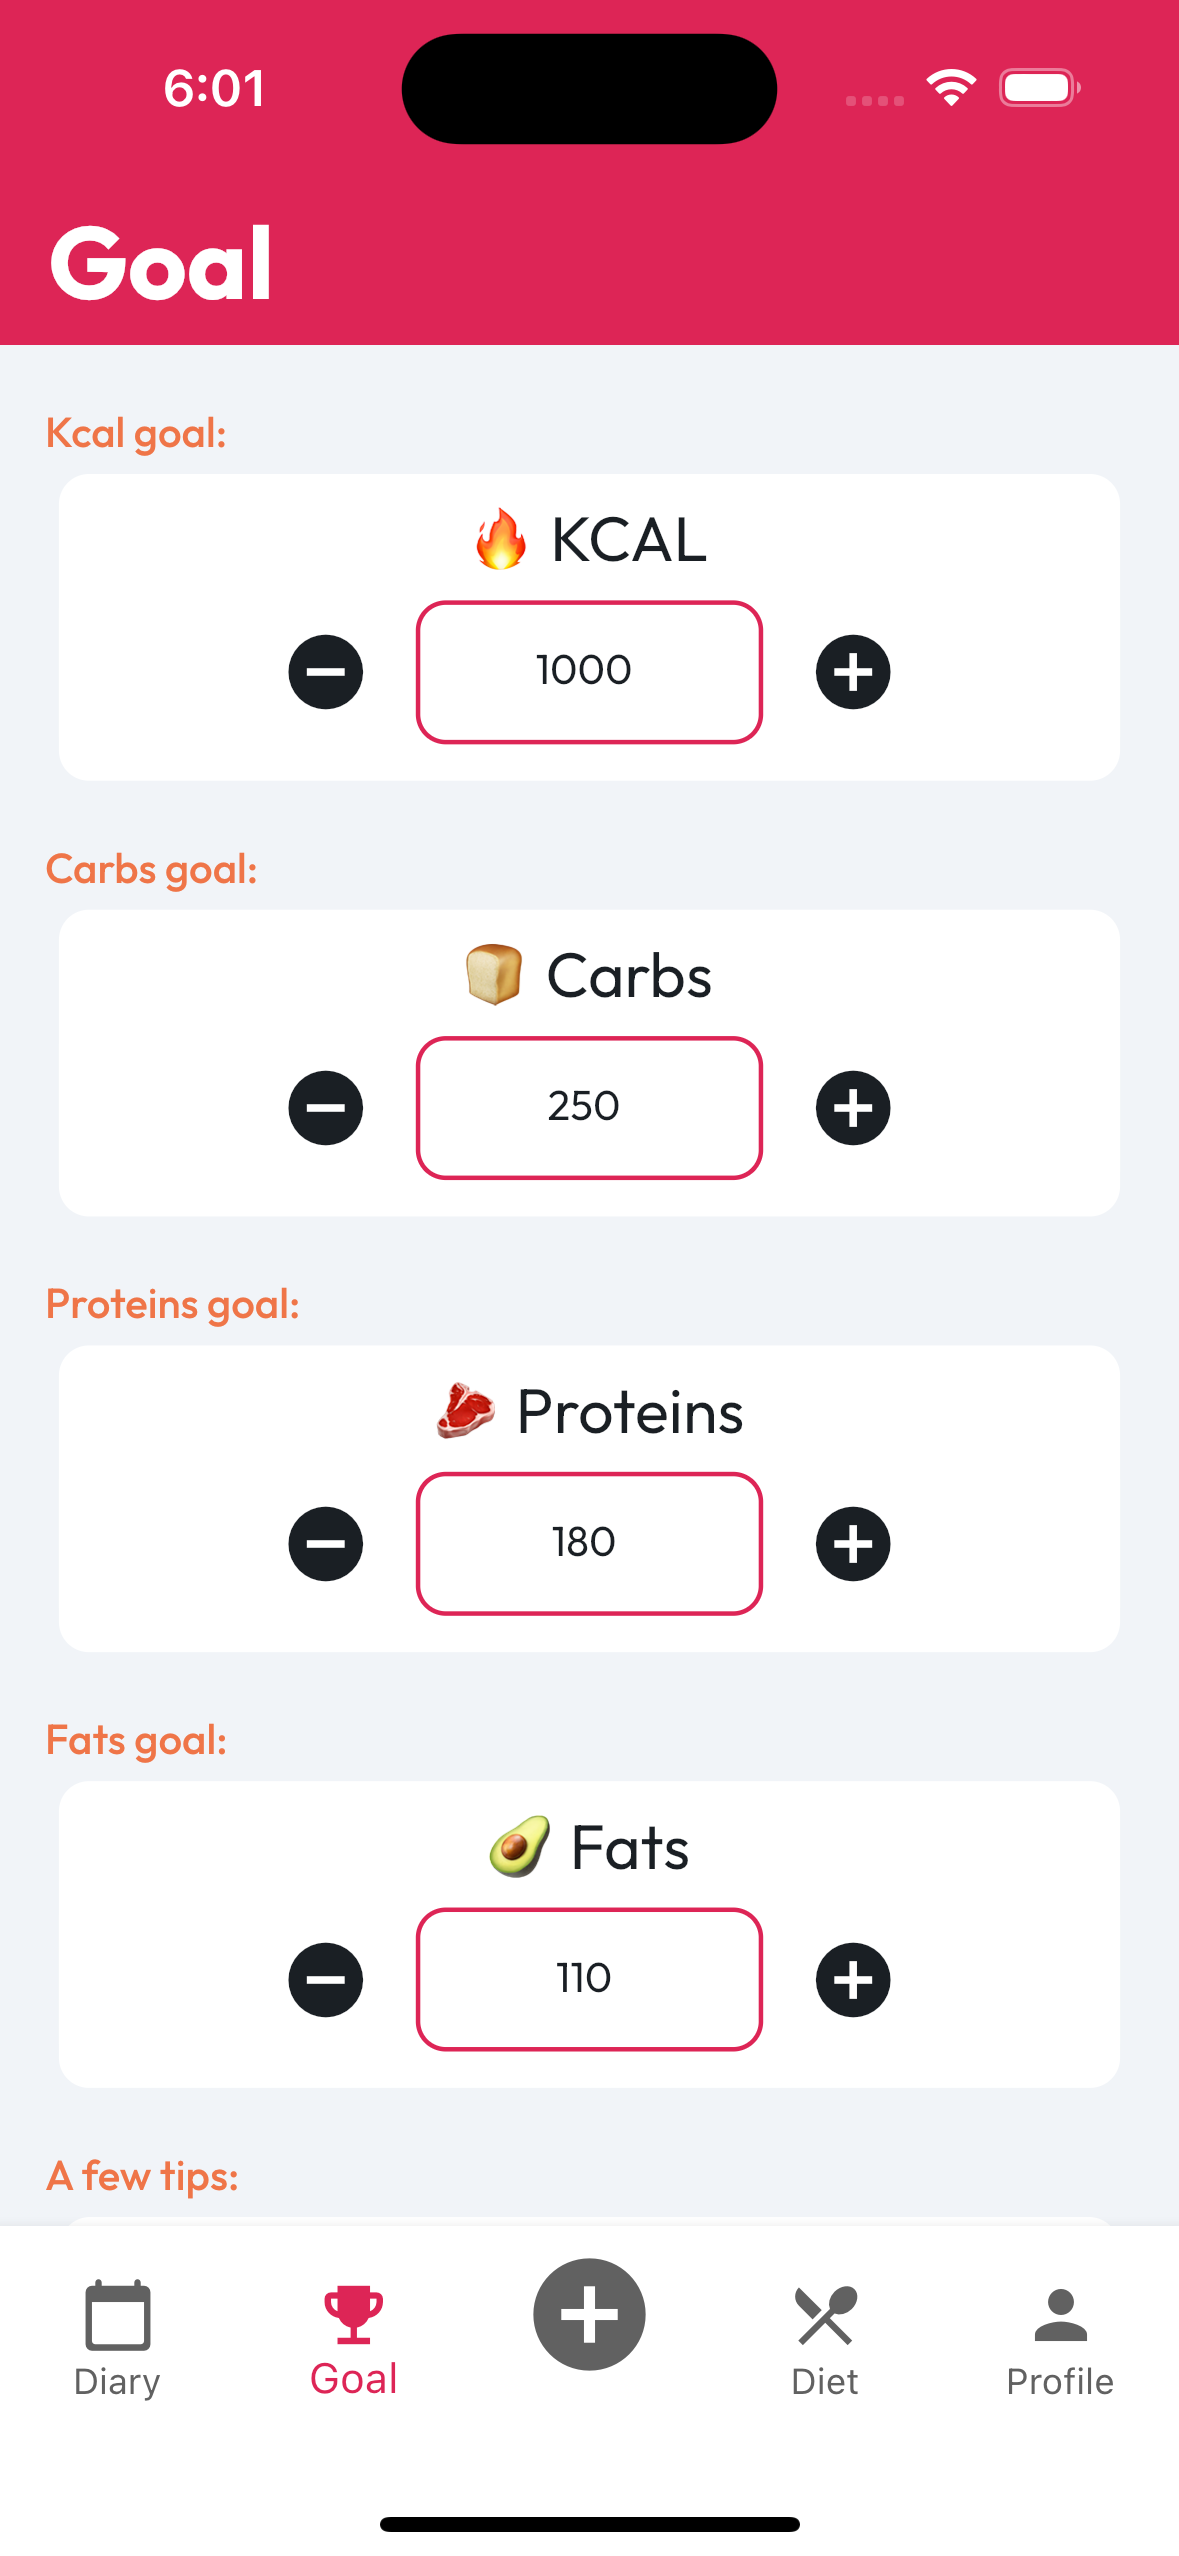
\includegraphics[scale=0.1]{Images/Screenshots/Mobile/Goal1Light.png}
  \caption{Goal page (1 of 2)}
\end{figure}

\begin{figure}[!h]
  \centering
  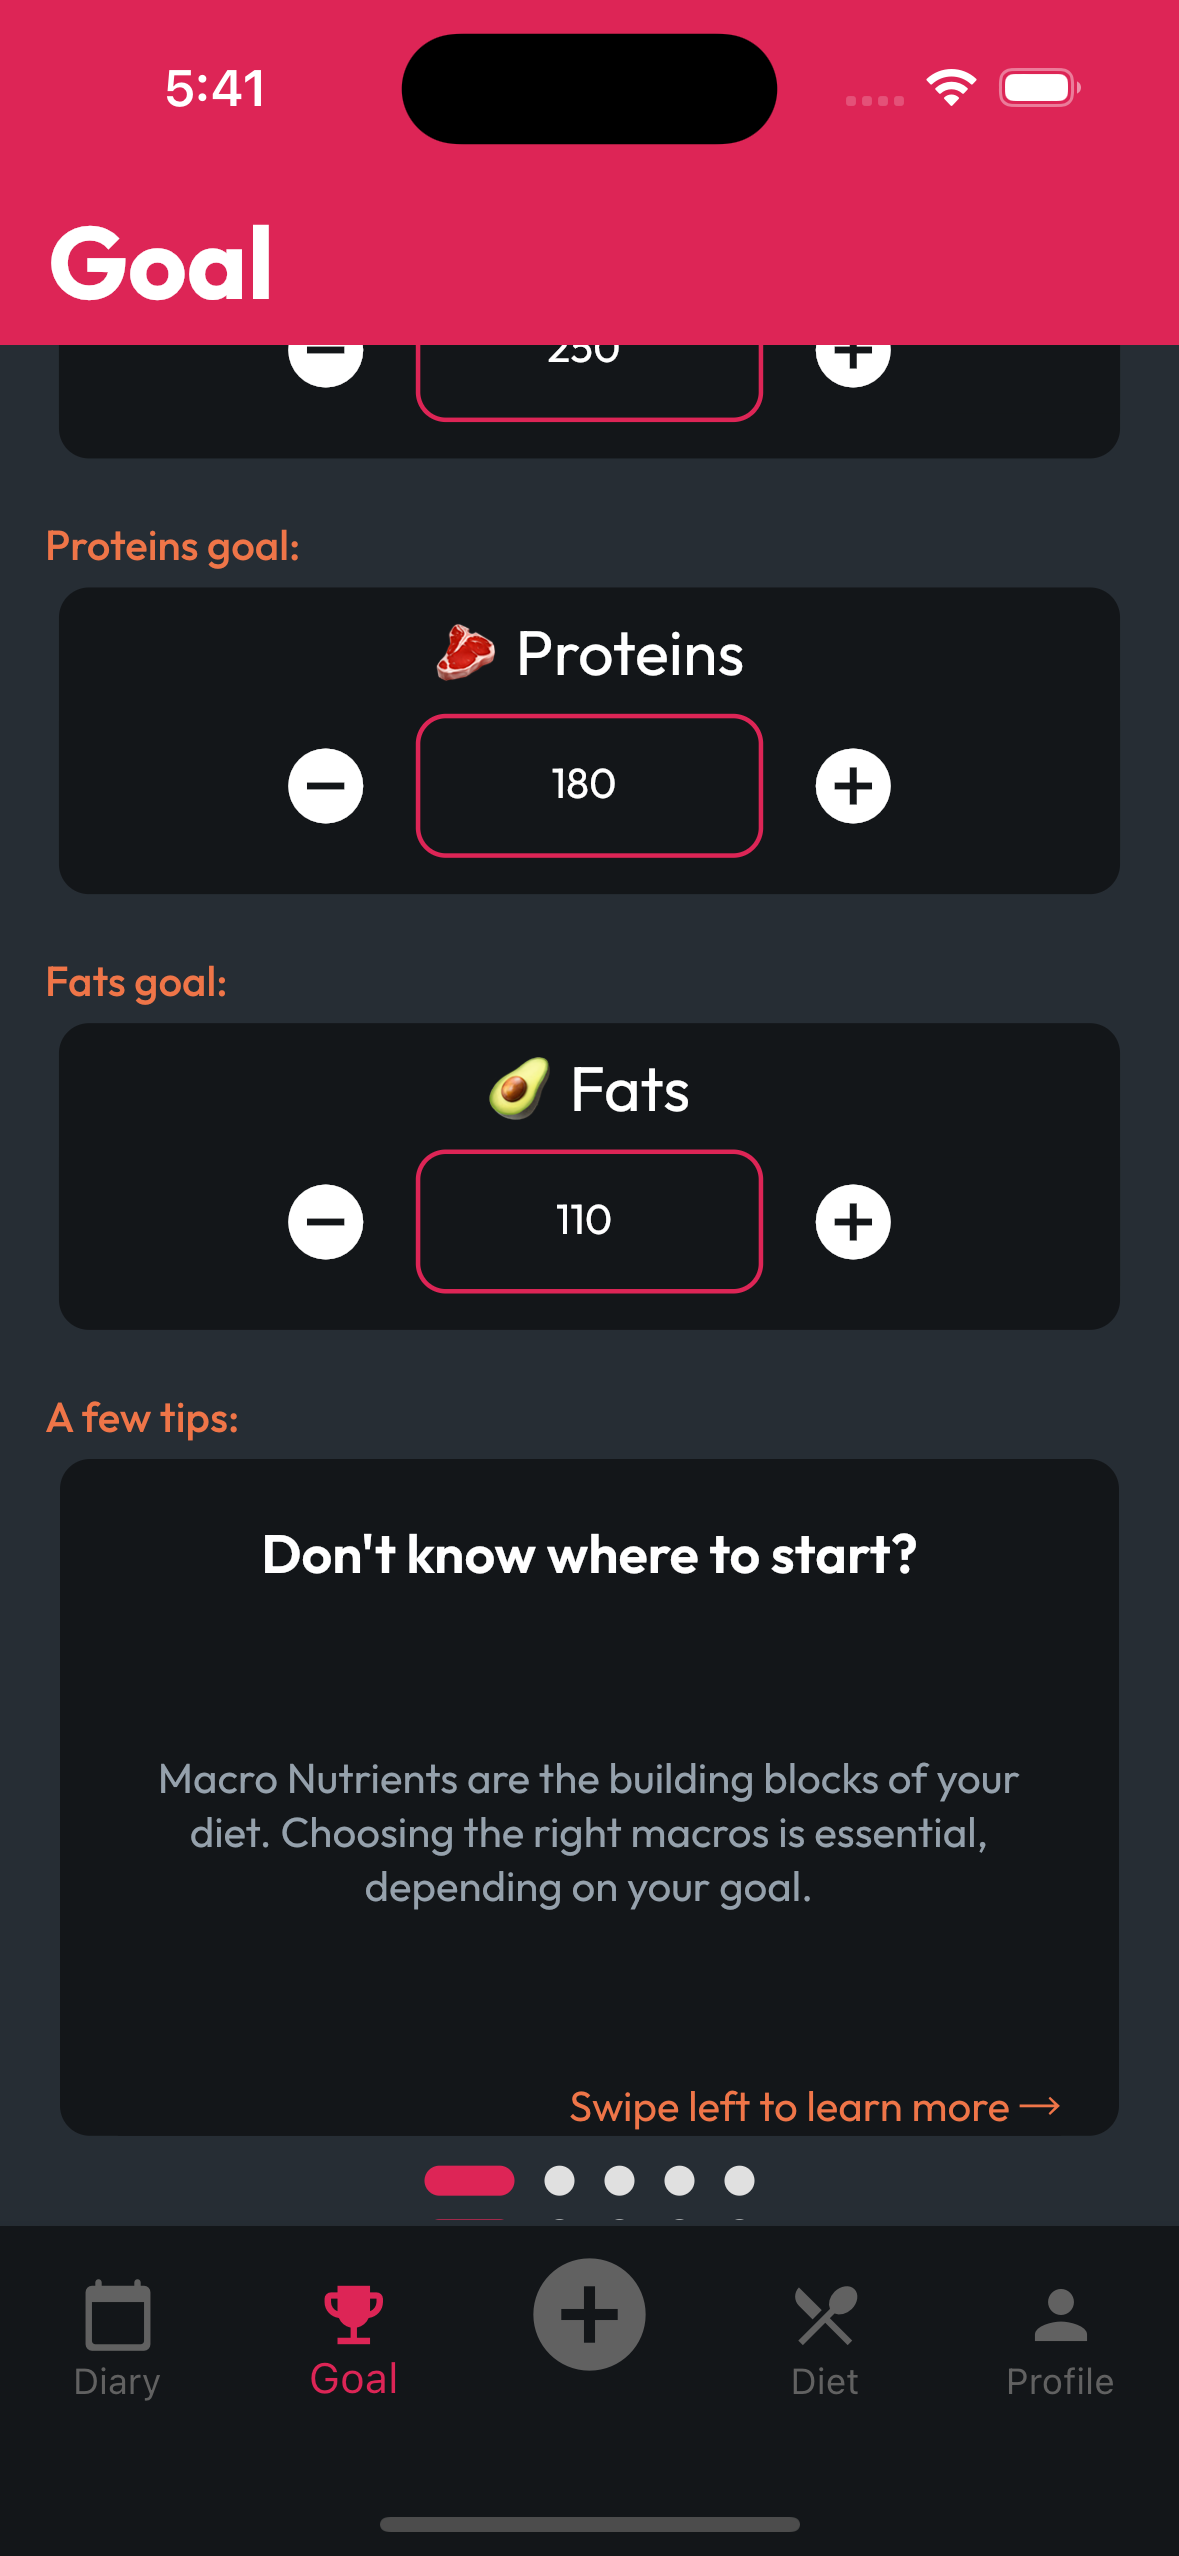
\includegraphics[scale=0.1]{Images/Screenshots/Mobile/Goal2.png}
  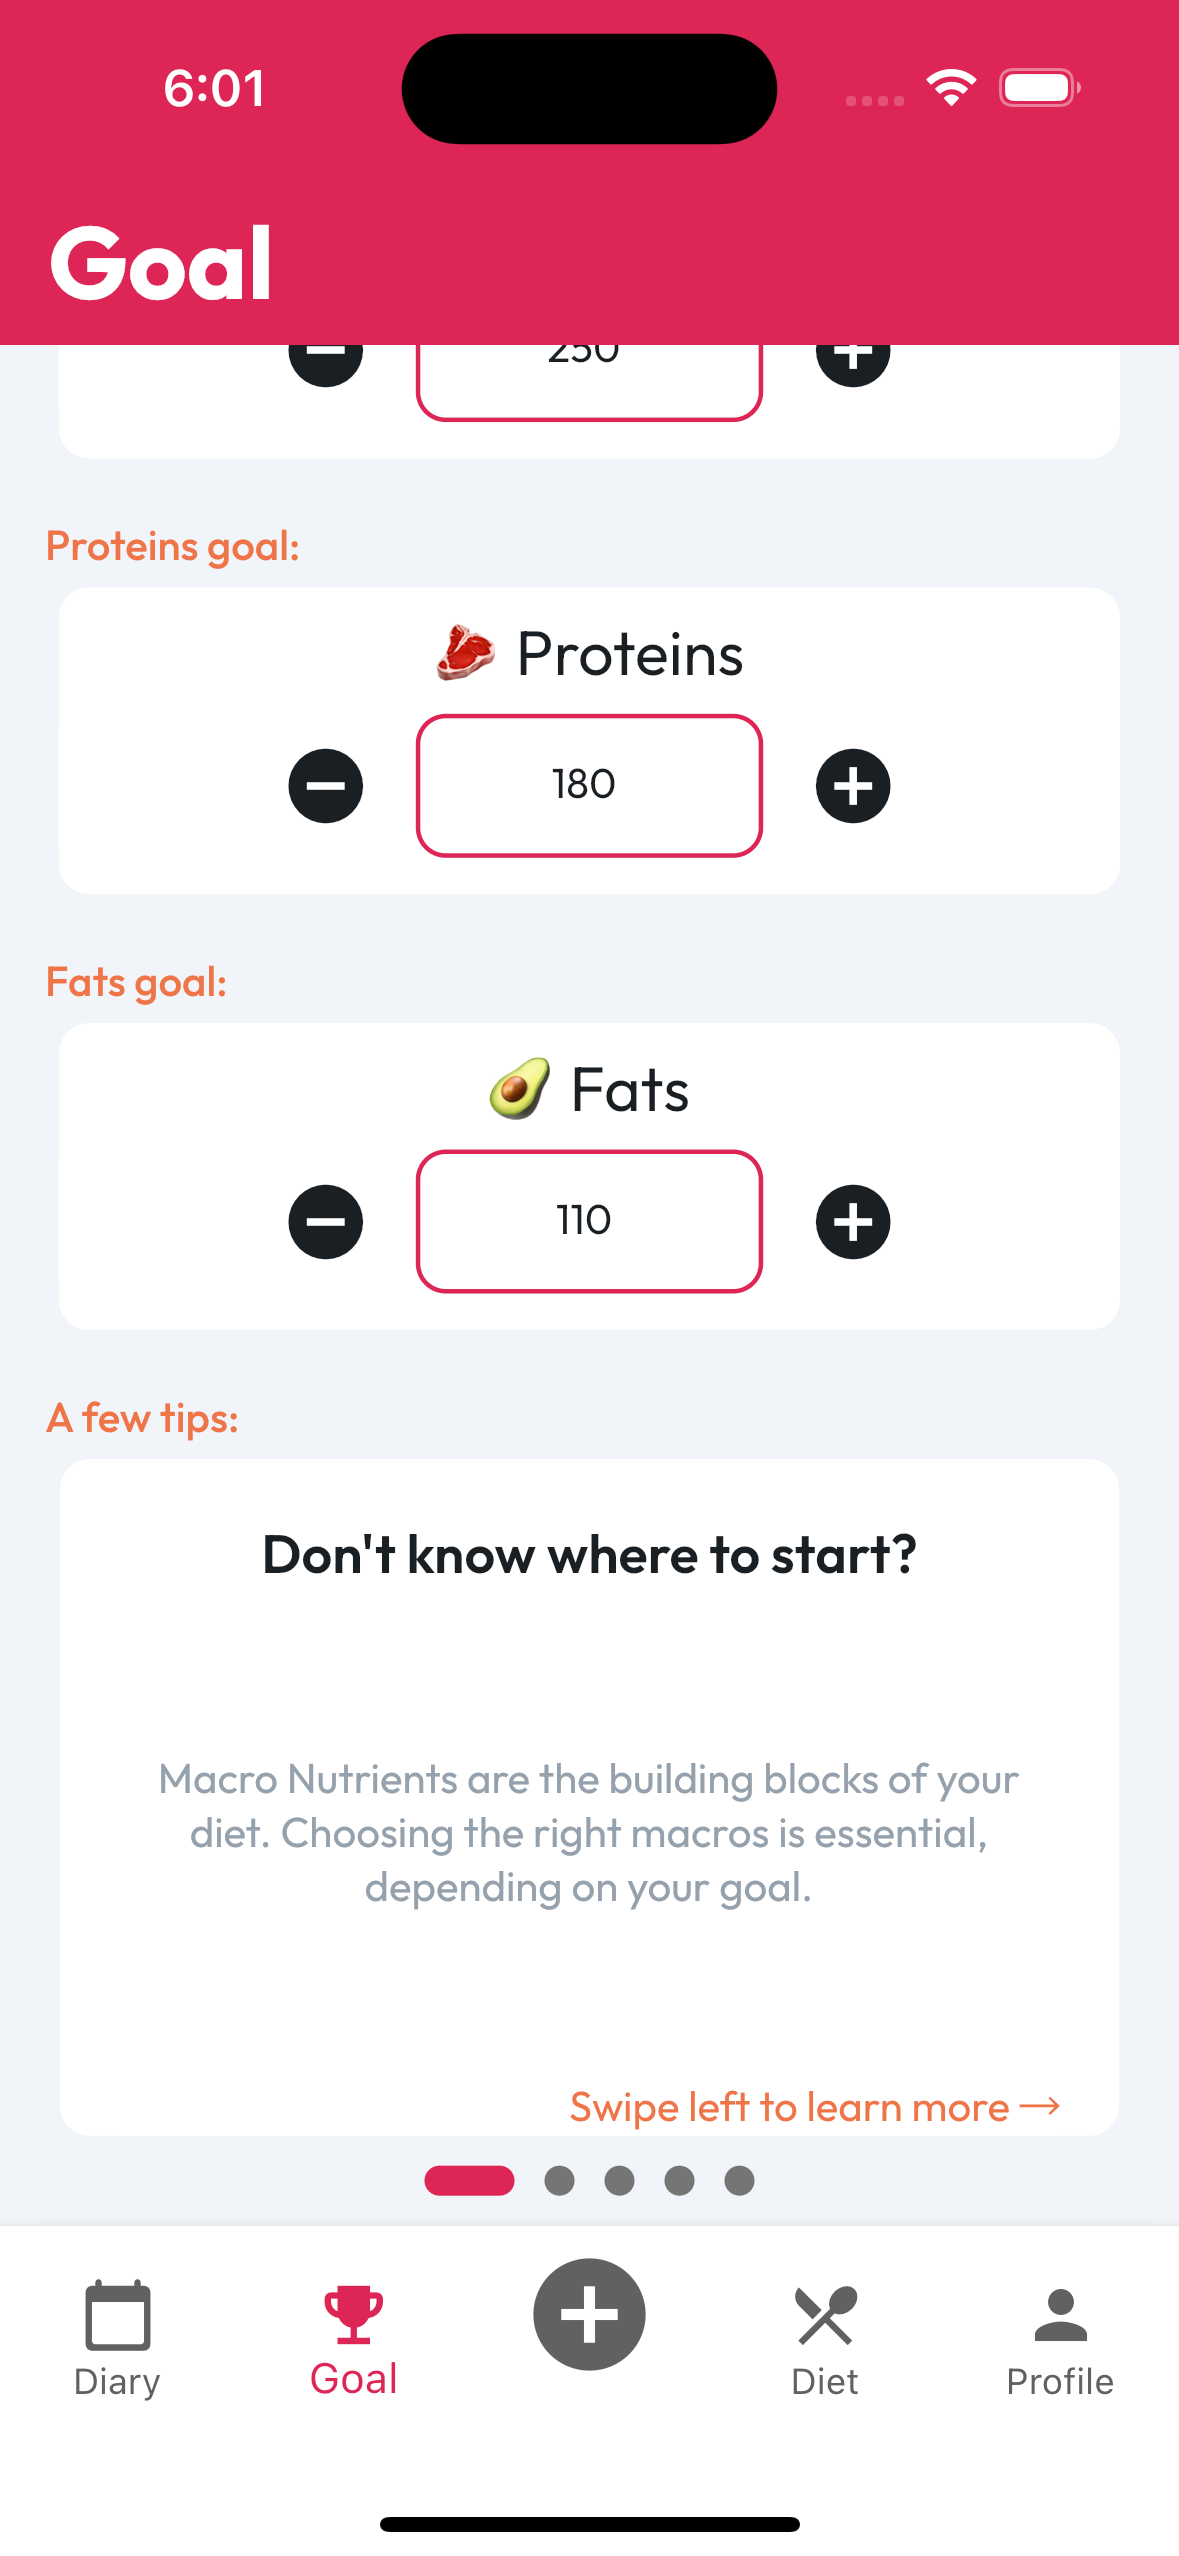
\includegraphics[scale=0.1]{Images/Screenshots/Mobile/Goal2Light.png}
  \caption{Goal page (2 of 2)}
\end{figure}

\clearpage

\subsection{Add page}

\begin{minipage}{\linewidth}
    This page shows the main methods to add a new food to the user daily diary or to the list of saved foods in the diet. Below there is a list of the foods registered the previous day in order to speed up the UX add procedure if the user wants to add a food inserted the day before.
\end{minipage}

\begin{figure}[!h]
  \centering
  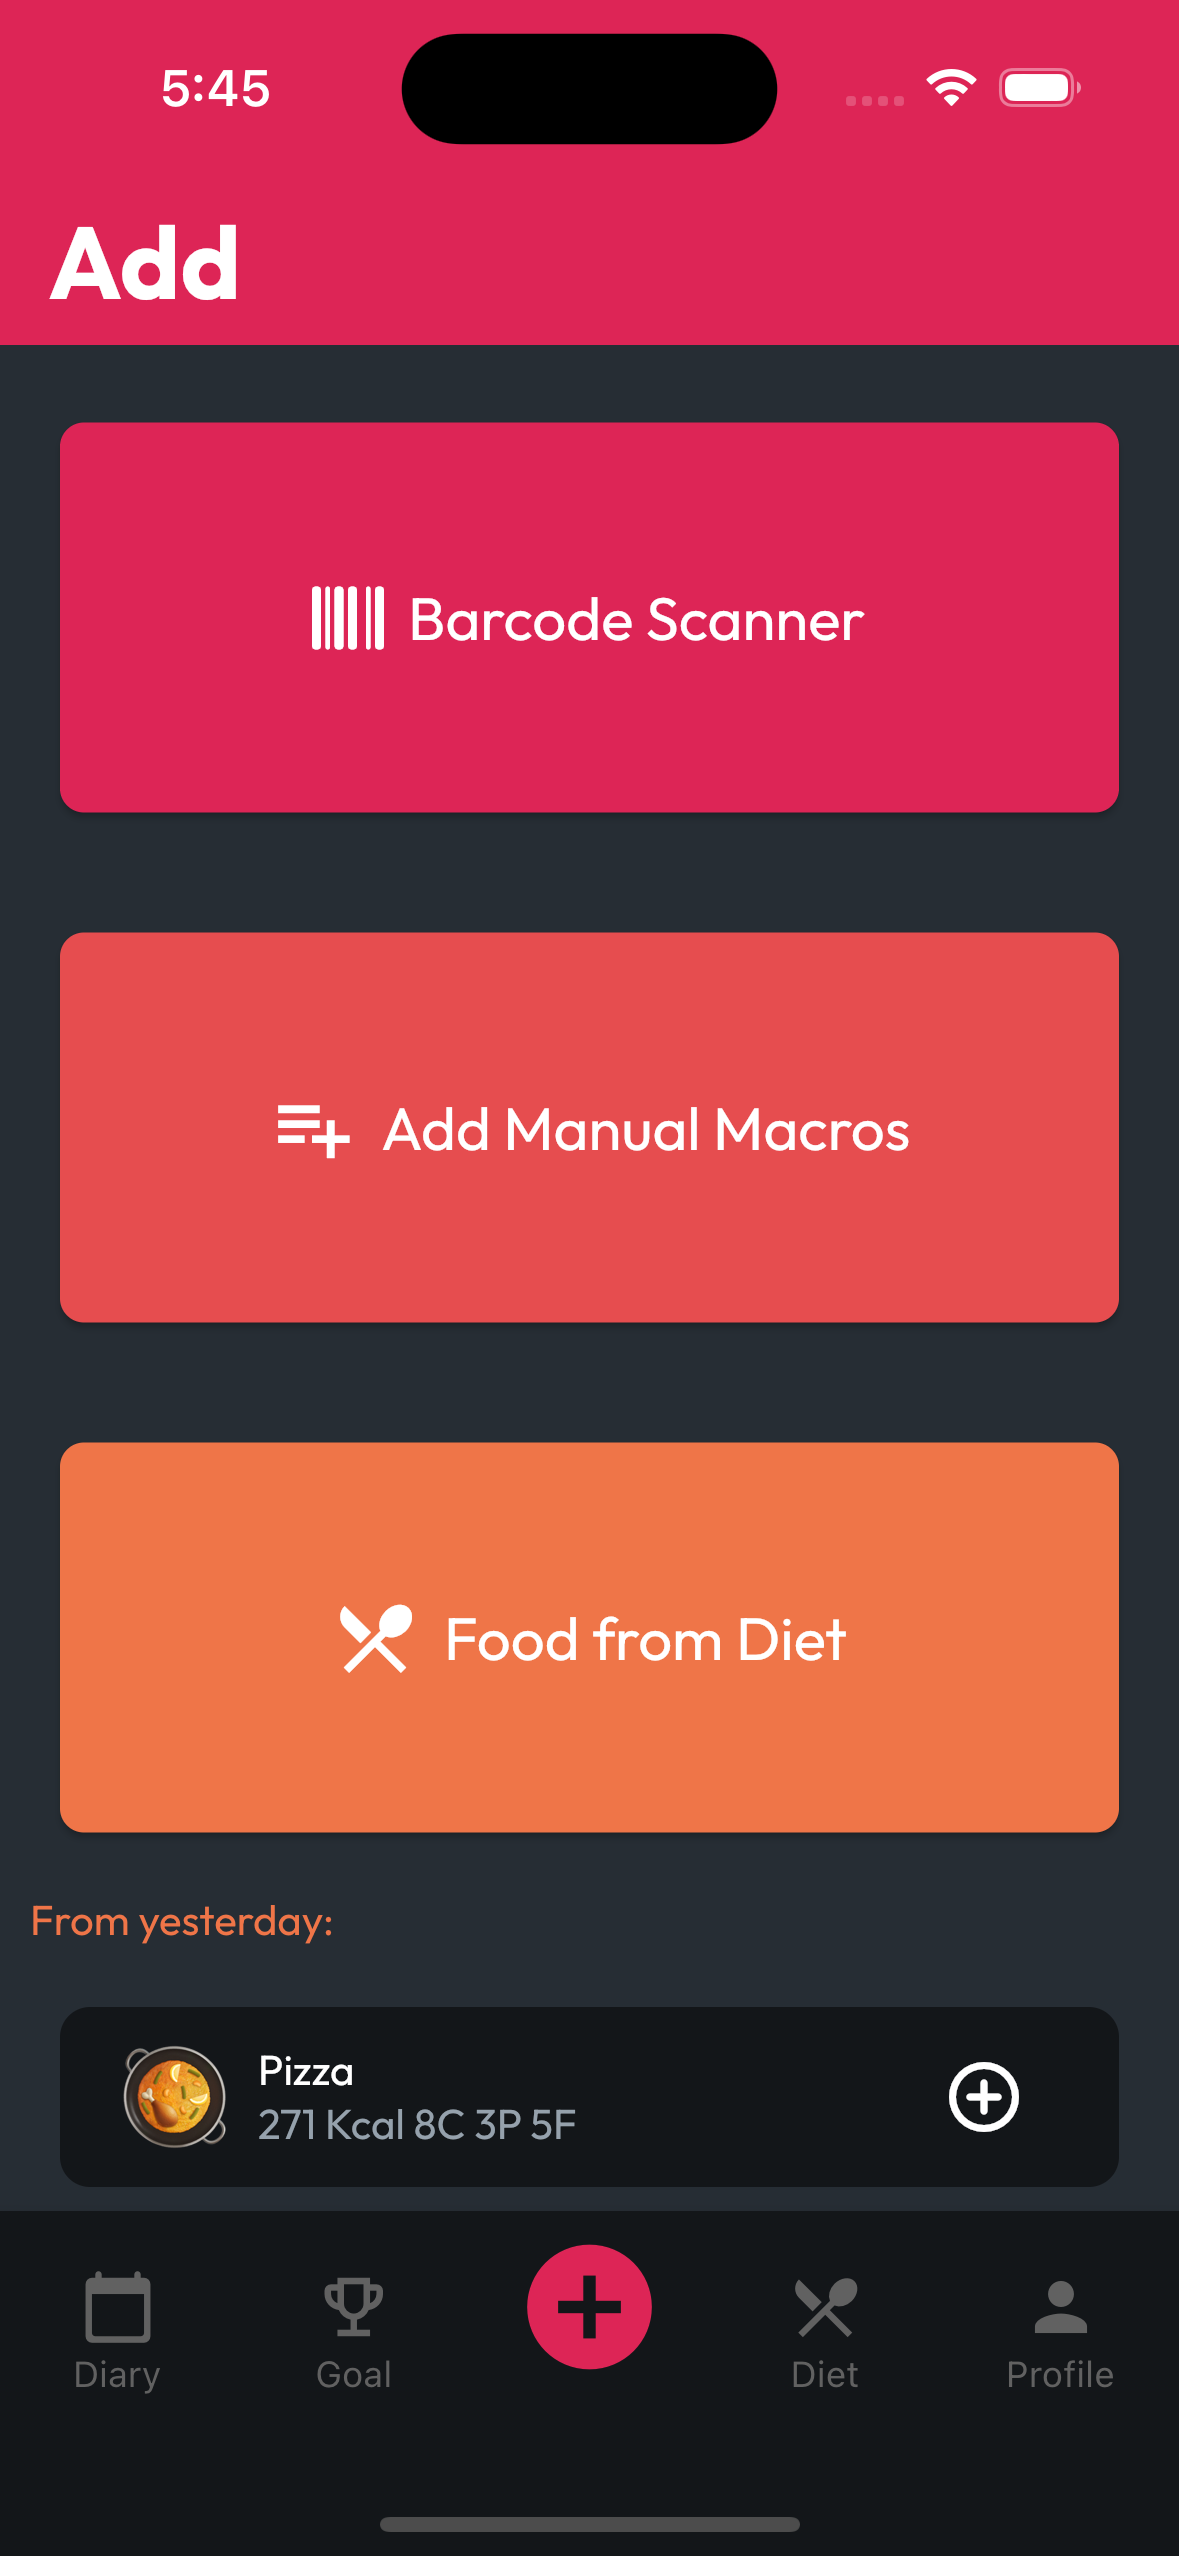
\includegraphics[scale=0.1]{Images/Screenshots/Mobile/Add.png}
  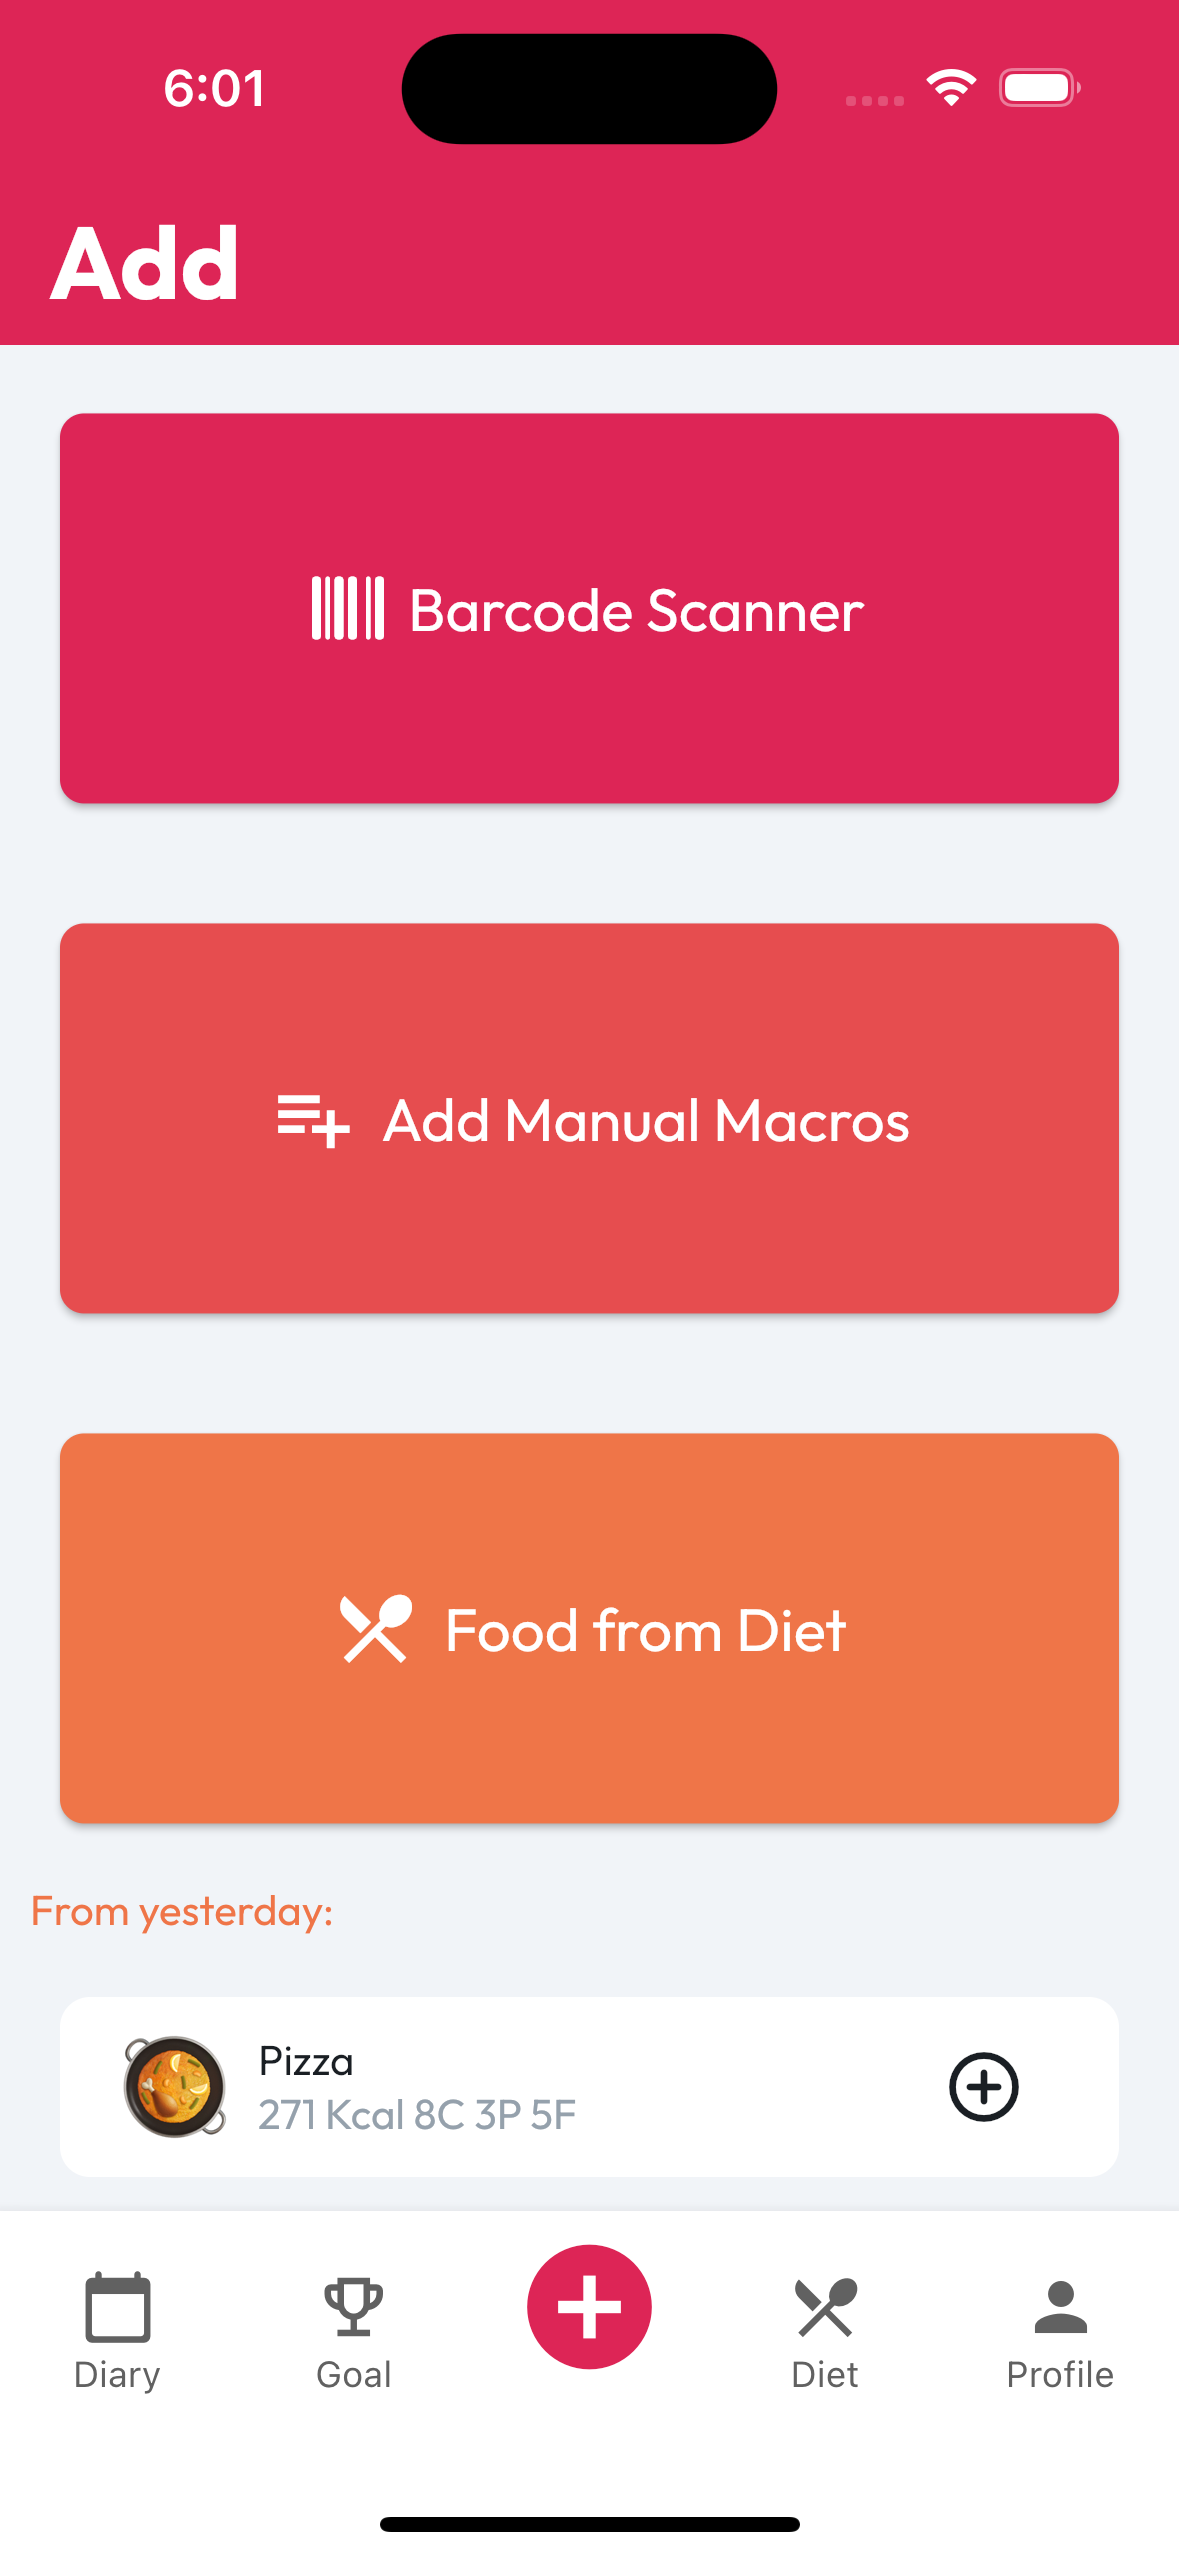
\includegraphics[scale=0.1]{Images/Screenshots/Mobile/AddLight.png}
  \caption{Add page}
\end{figure}

\clearpage

\subsection{Scan barcode page}

\begin{minipage}{\linewidth}
    Page for scanning foods' barcode. It let the user choose whether to use the front or the retro camera and using or not the flash.
\end{minipage}

\begin{figure}[!h]
  \centering
  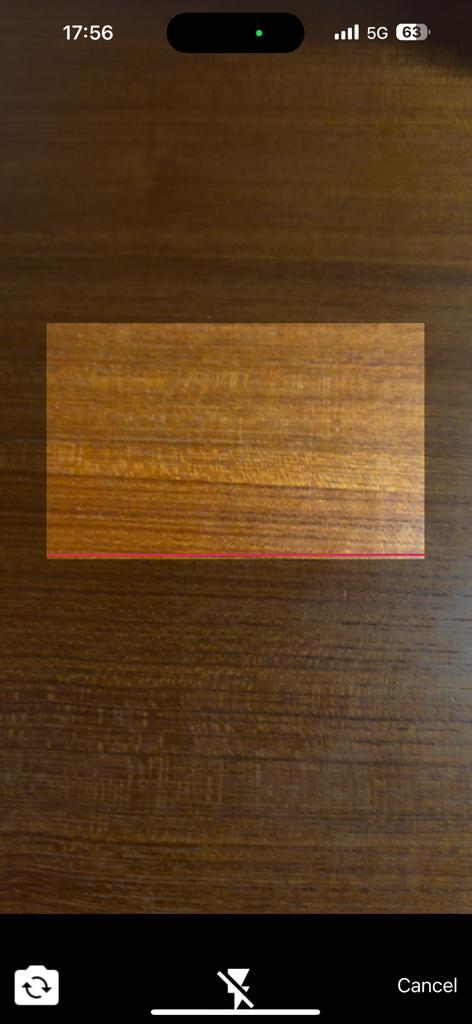
\includegraphics[scale=0.3]{Images/Screenshots/Mobile/Barcode.jpeg}
  \caption{Scan barcode page}
\end{figure}

\begin{minipage}{\linewidth}
    \textbf{Note}: after the scan the app let the user insert the quantity of the food with the \emph{Add food} page, or displays an alert if it doesn't find the food.
\end{minipage}

\clearpage

\subsection{Diet page}

\begin{minipage}{\linewidth}
    This page displays the list of foods inserted in the user diet. For each food (tile) the user can edit the food already inserted or add it to the daily diary.  \\
    By clicking on the meal types (e.g. Breakfast, Lunch, Dinner, Snack), the user can filter the foods to show a restricted list. \\
    On the top right there is the \emph{Add custom food} button that enables the user to insert a new food.
\end{minipage}

\begin{figure}[!h]
  \centering
  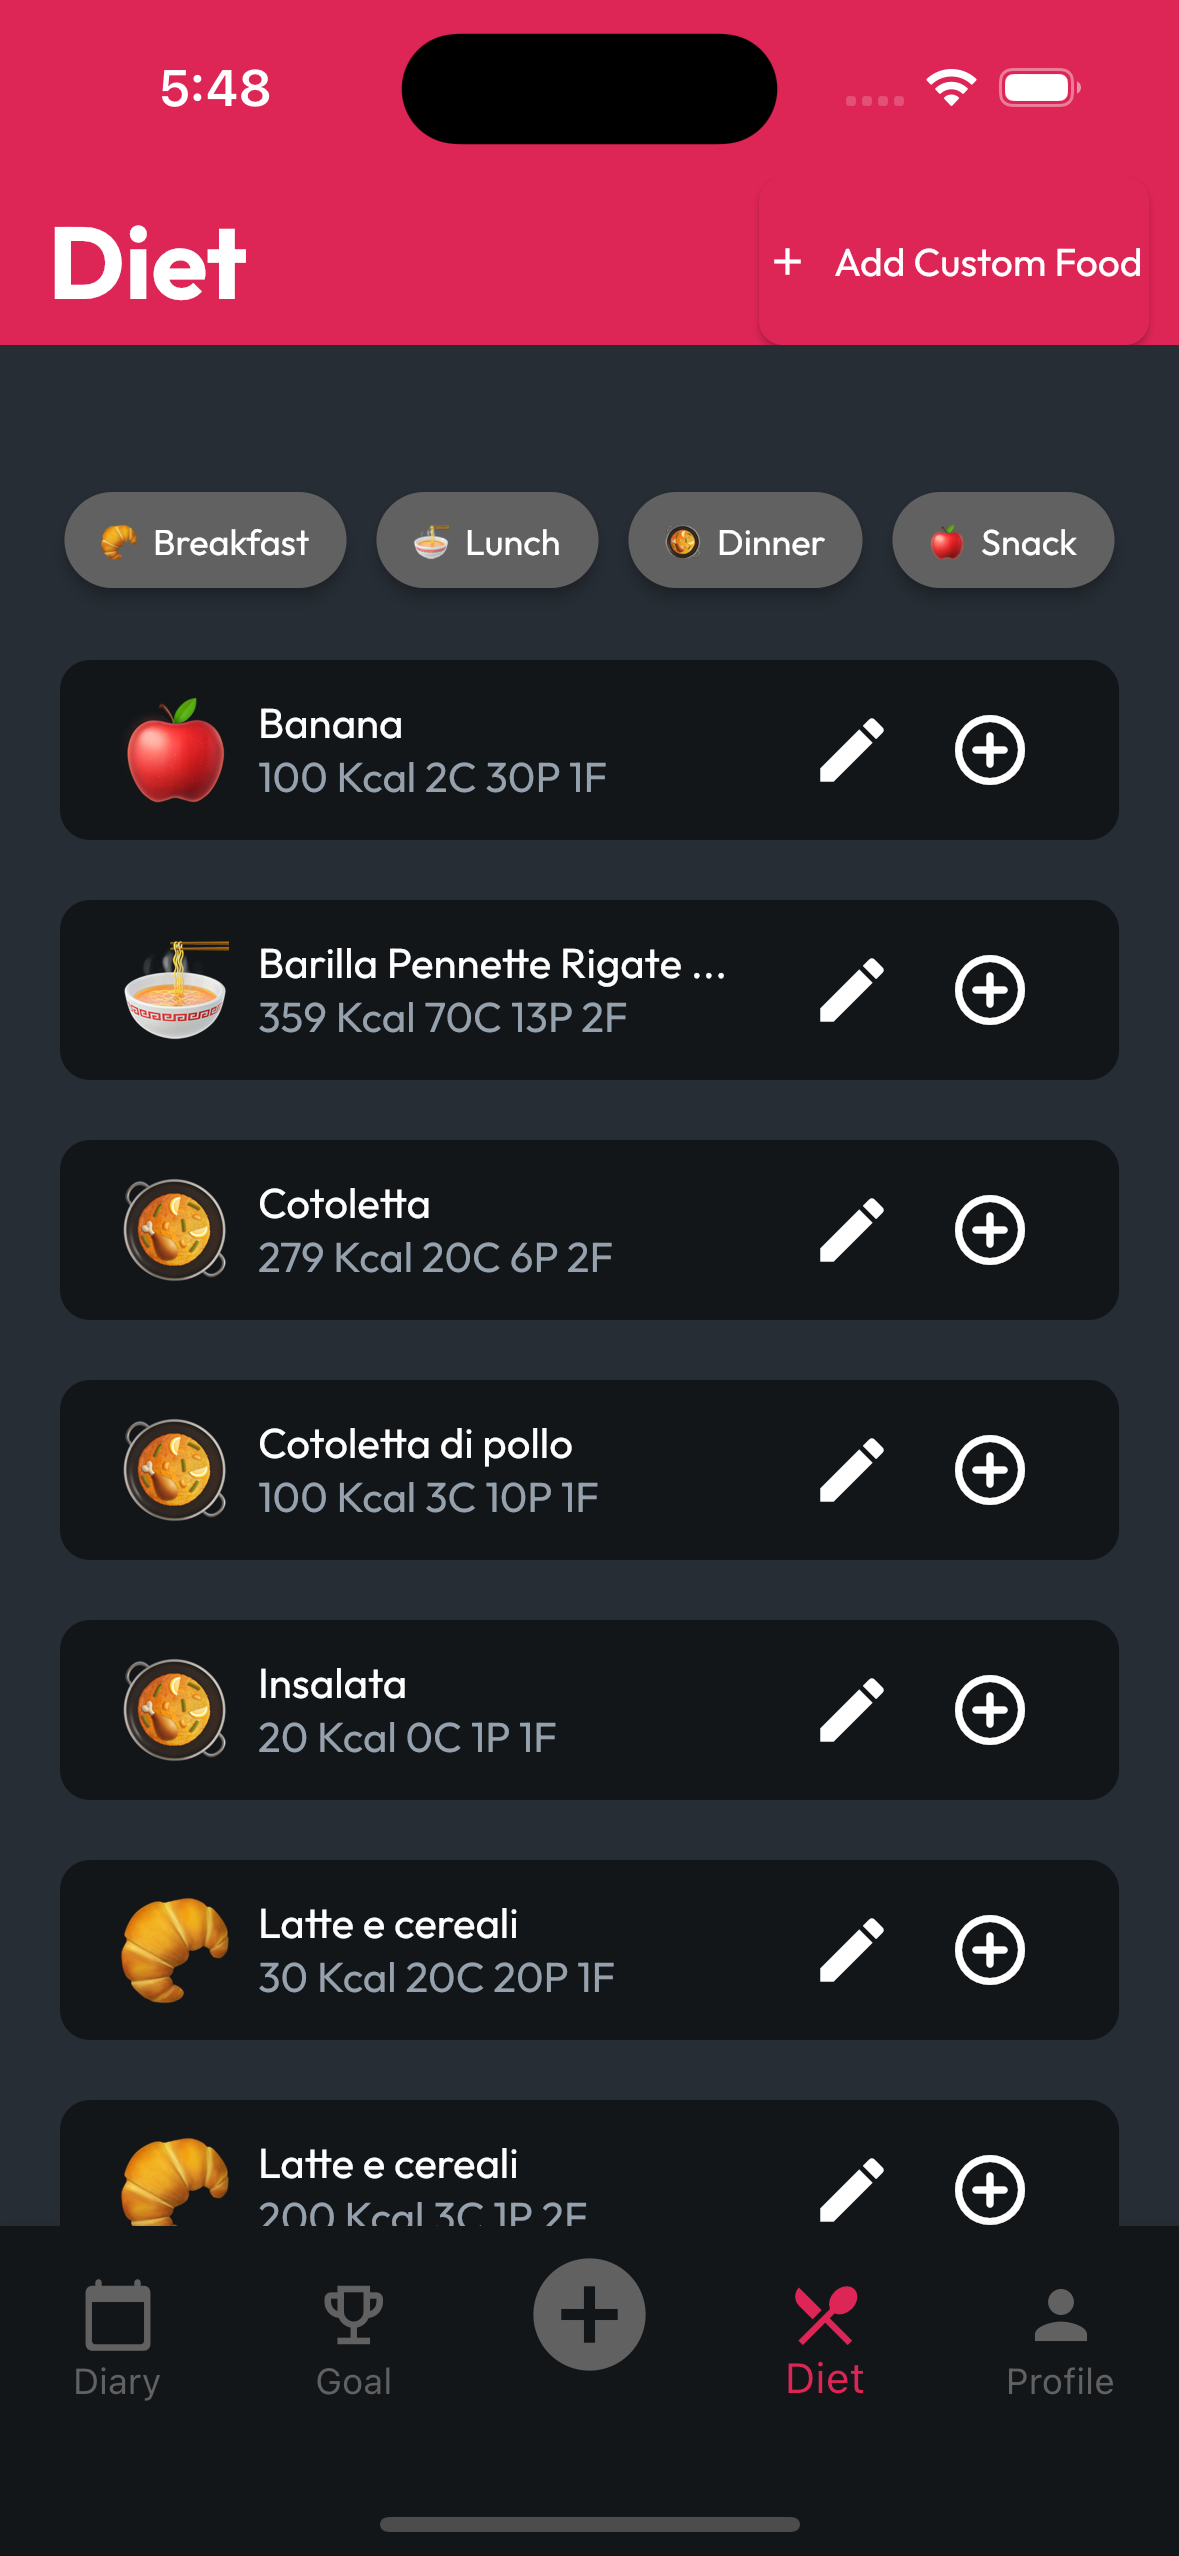
\includegraphics[scale=0.1]{Images/Screenshots/Mobile/Diet.png}
  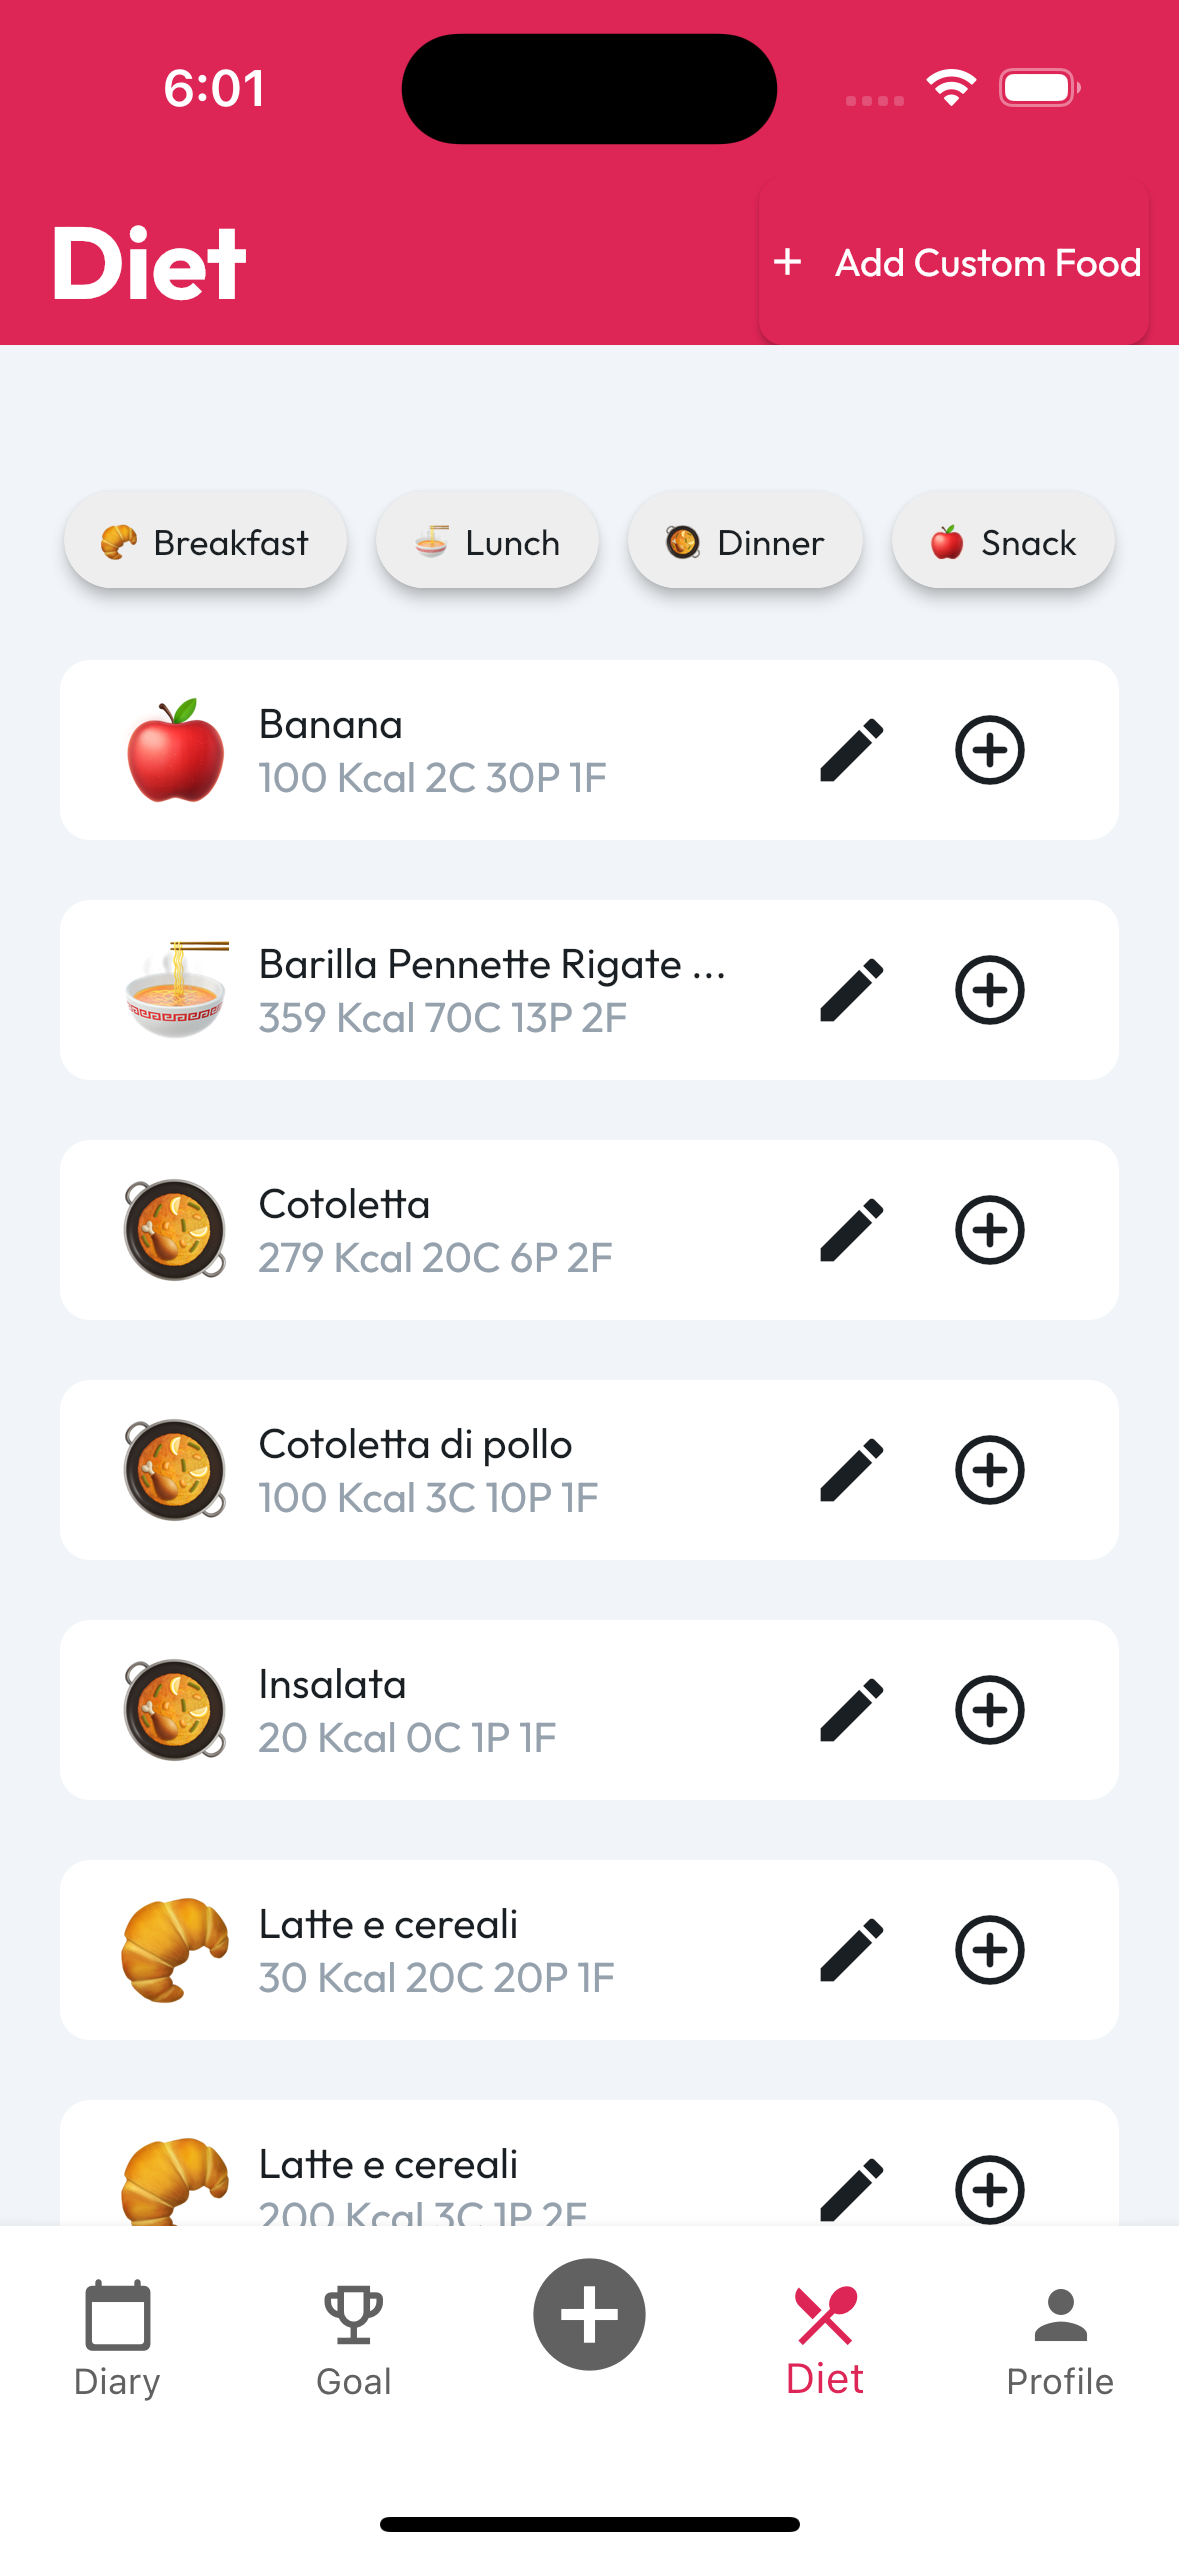
\includegraphics[scale=0.1]{Images/Screenshots/Mobile/DietLight.png}
  \caption{Diet page}
\end{figure}

\begin{figure}[!h]
    \centering
    
\includegraphics[scale=0.7]{Images/Screenshots/Mobile/DietFoodItem.png}
    \caption{Single tile of diet food.}
\end{figure}

\clearpage

\subsection{Add food page}

\begin{minipage}{\linewidth}
    This page is shown when clicking on the \emph{Add manual macros} or \emph{Add custom food} buttons. From there the user can submit all the custom properties of a food he wants to register.
    The \emph{Add to Diet} button adds the food to the user's diet; while the \emph{Log Food} adds it to the diary foods.
\end{minipage}

\begin{figure}[!h]
  \centering
  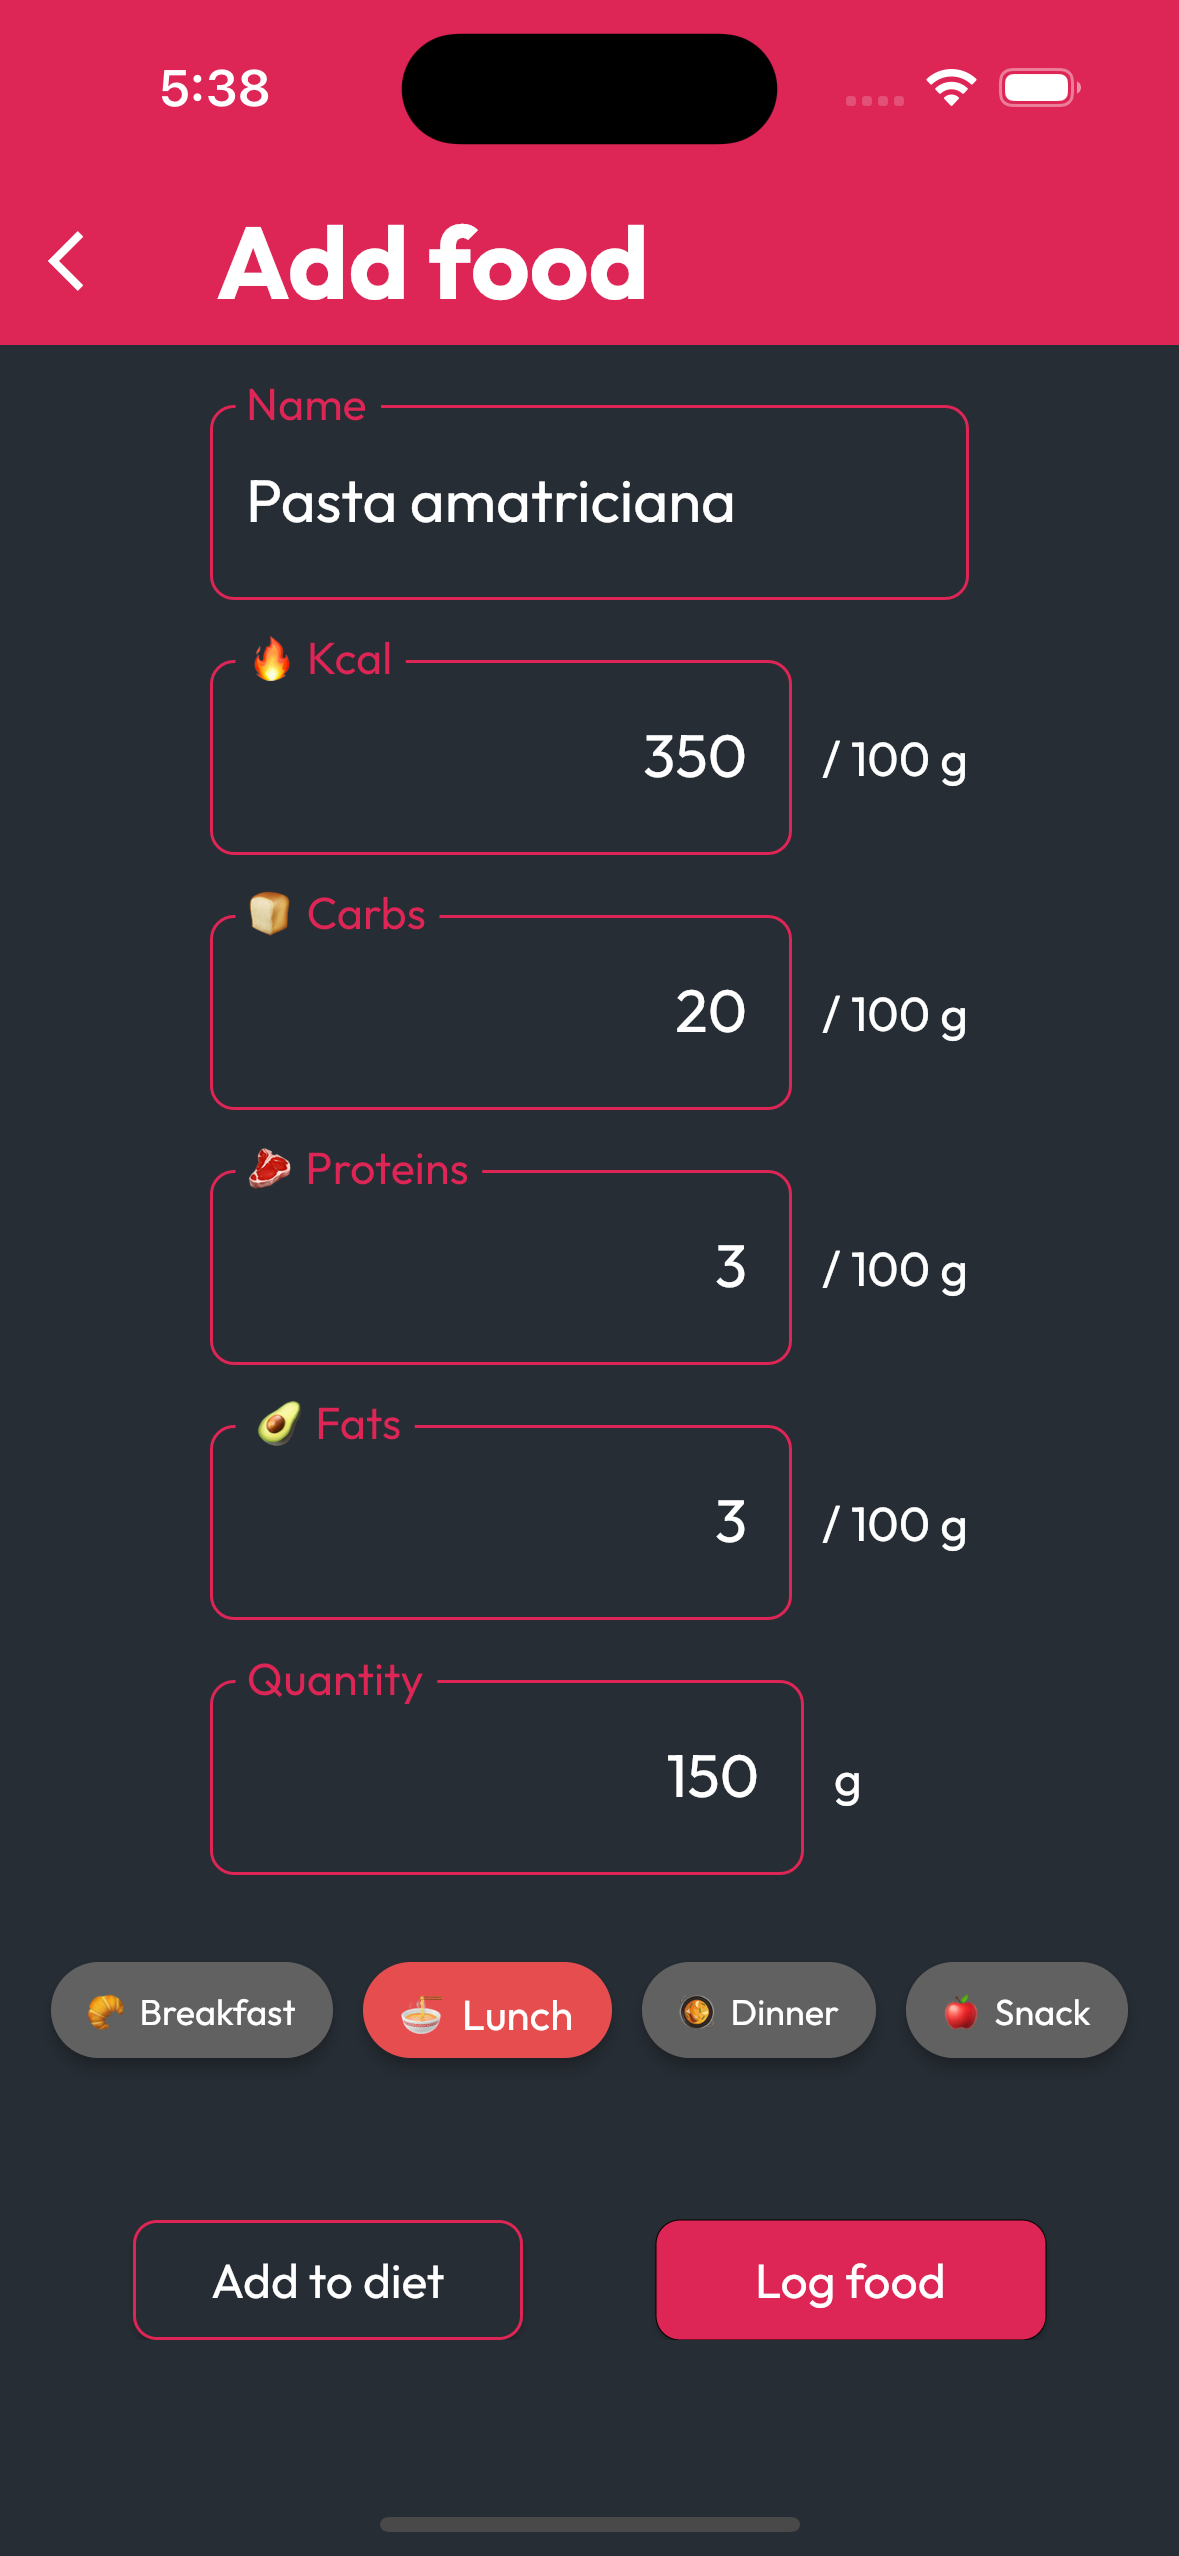
\includegraphics[scale=0.1]{Images/Screenshots/Mobile/AddFood.png}
  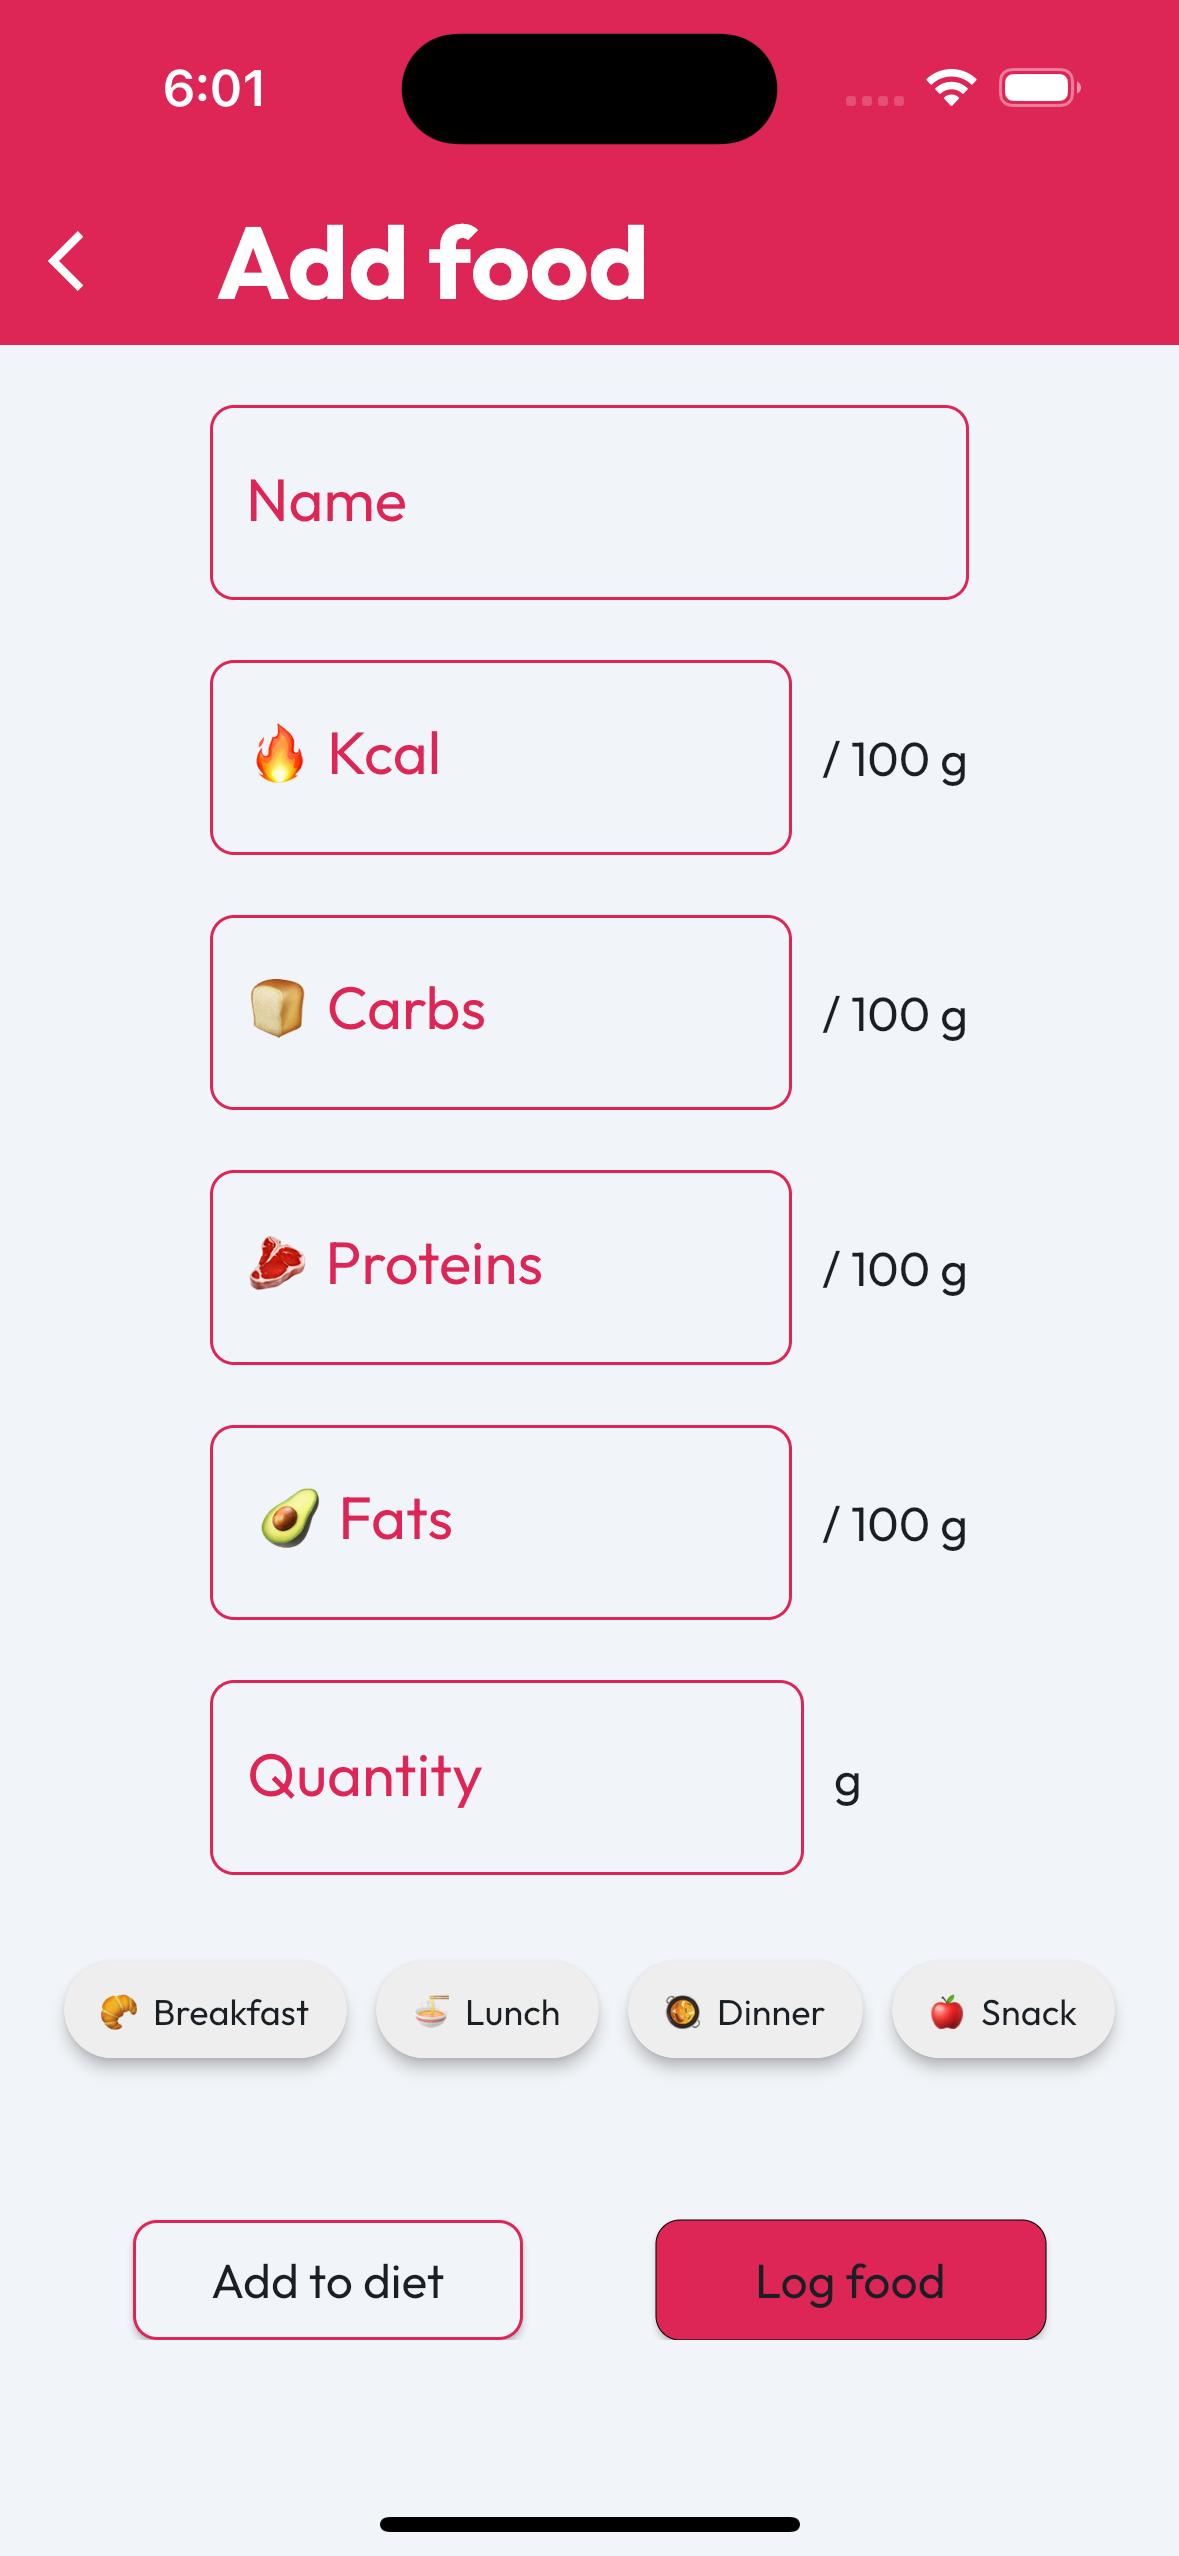
\includegraphics[scale=0.1]{Images/Screenshots/Mobile/AddFoodLight.png}
  \caption{Add food page}
\end{figure}

\clearpage

\subsection{Profile page}

\begin{minipage}{\linewidth}
    This screen contains the settings of the app and the user information.
    In detail it greets the user with a "\emph{Welcome}" followed by the user name, and a set of settings for update user's information.\\
    It gives the possibility to switch to light/dark mode and to log out from the app with a button.
\end{minipage}

\begin{figure}[!h]
  \centering
  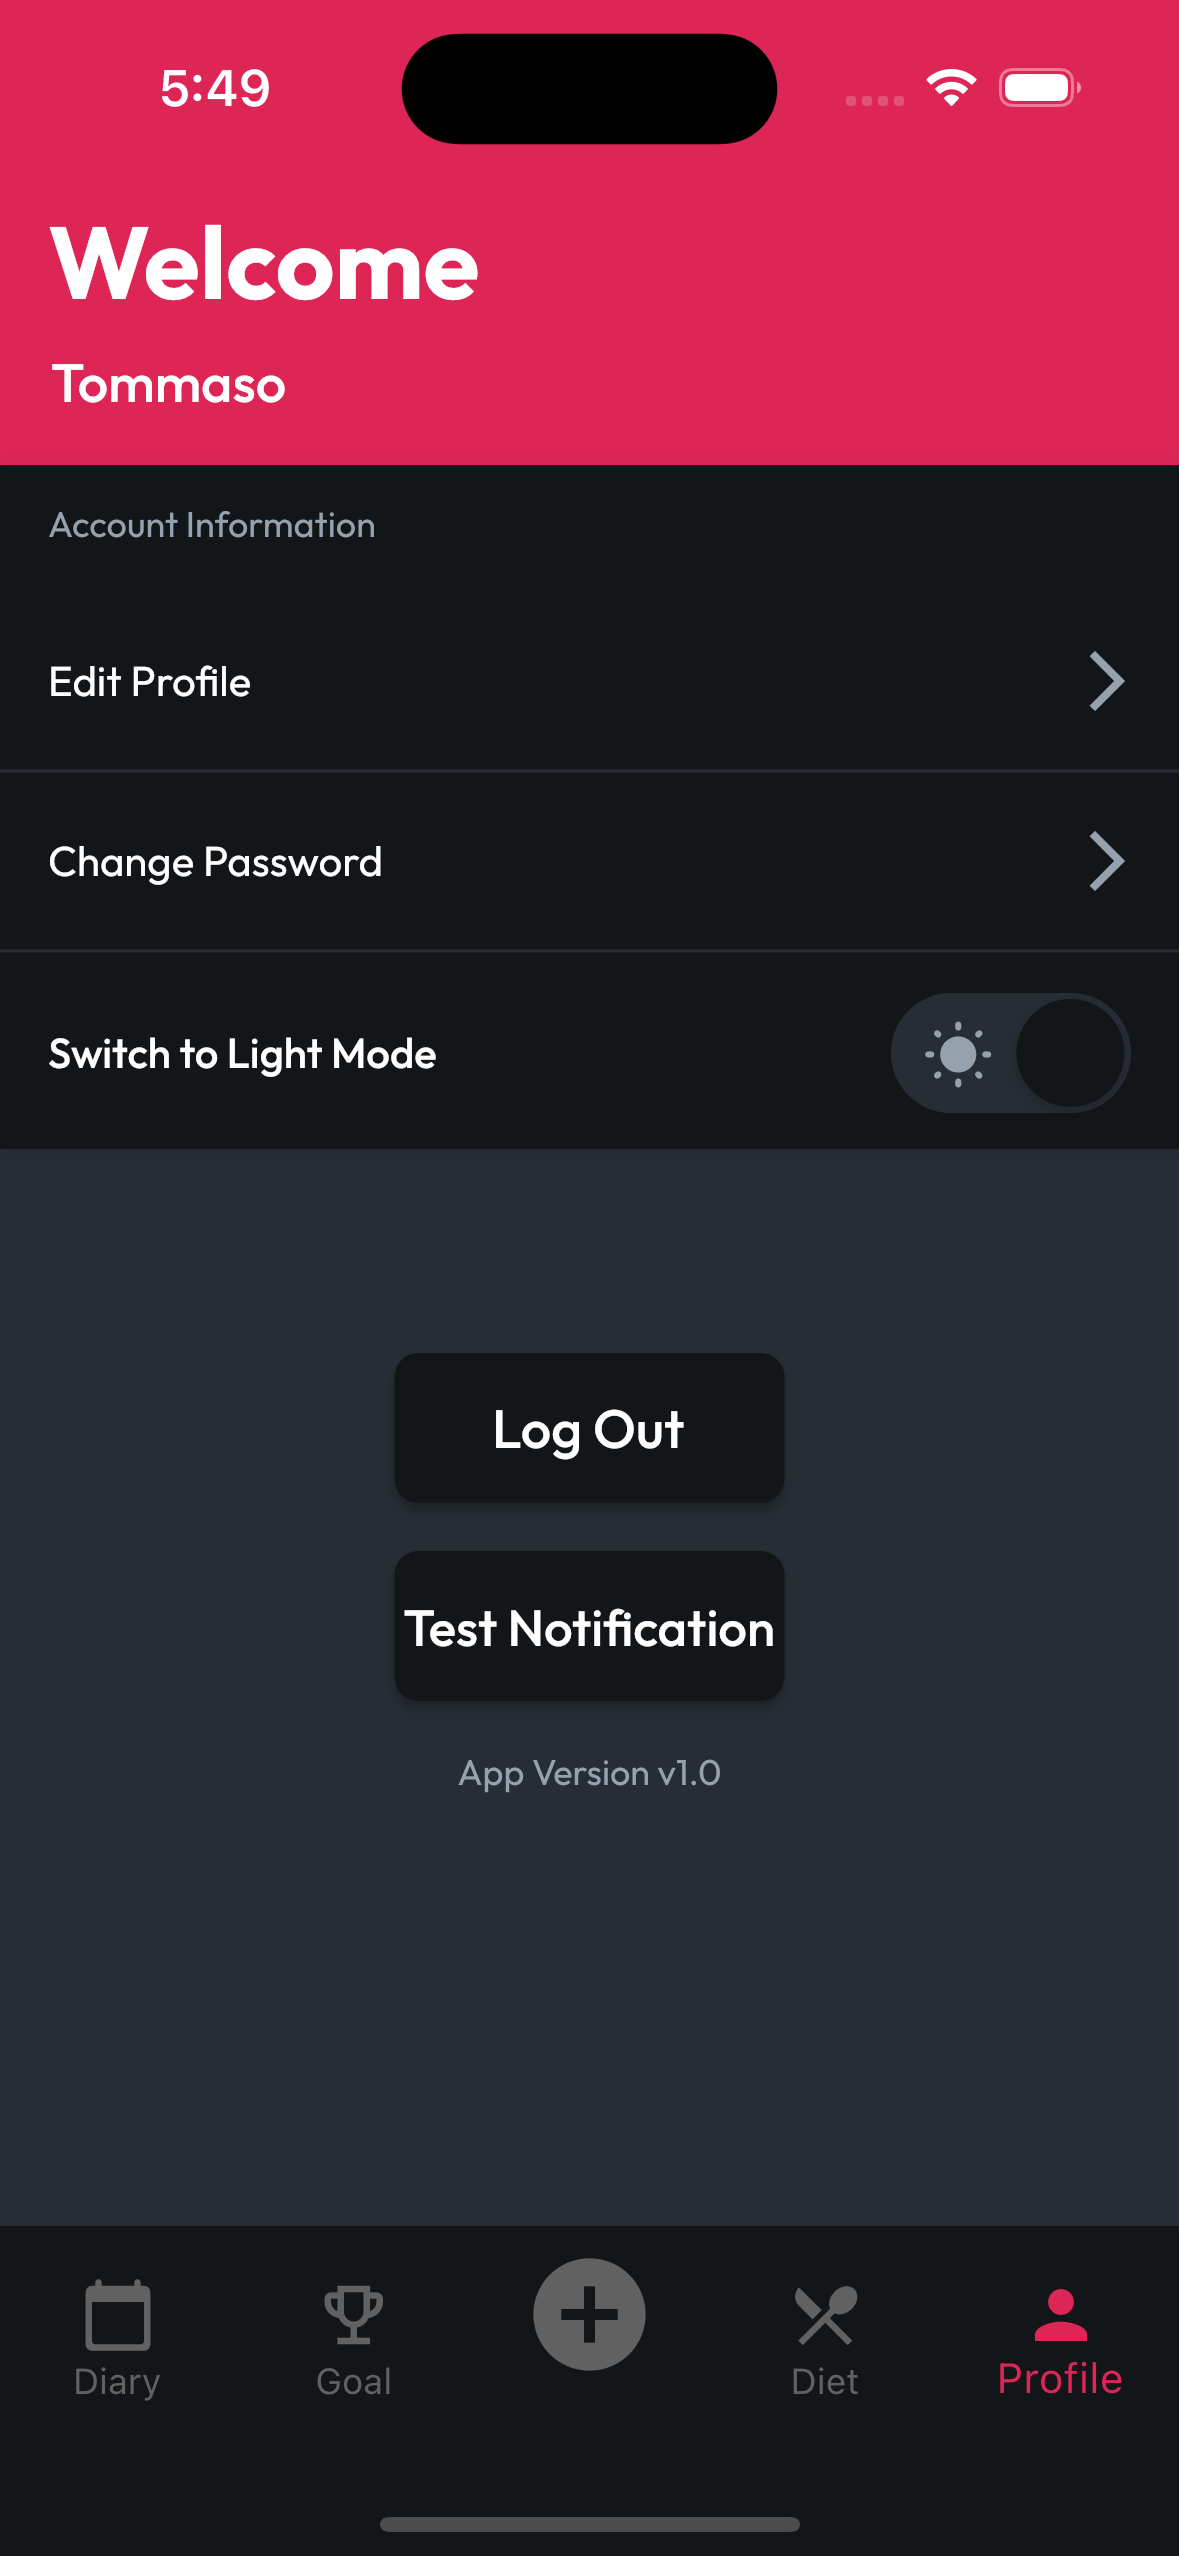
\includegraphics[scale=0.1]{Images/Screenshots/Mobile/Profile.png}
  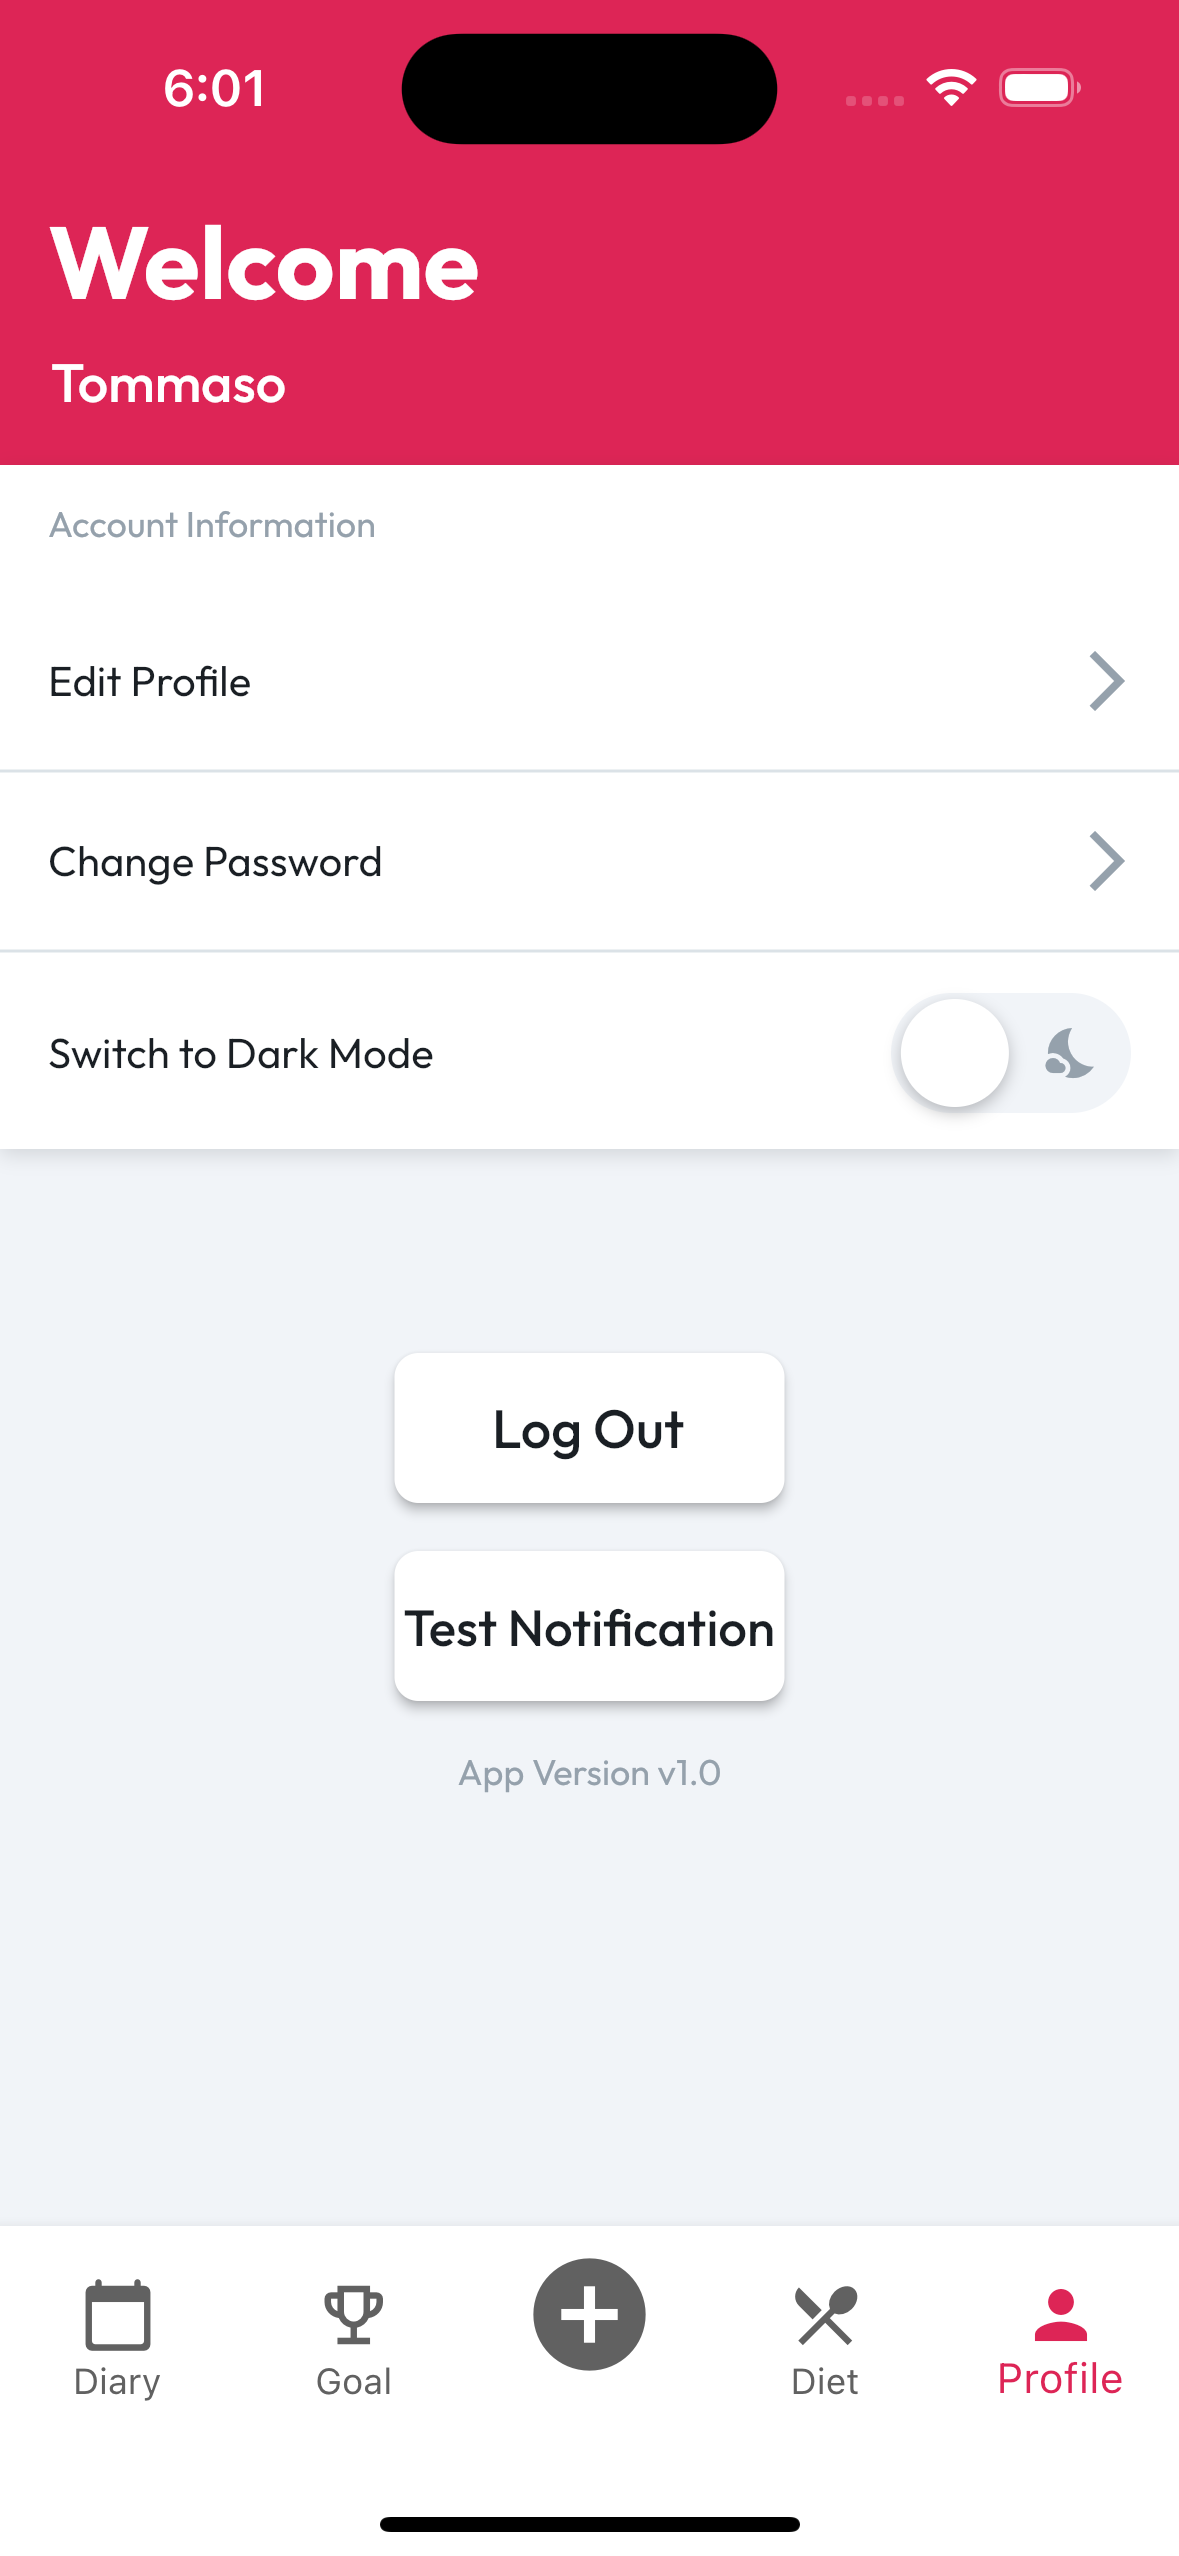
\includegraphics[scale=0.1]{Images/Screenshots/Mobile/ProfileLight.png}
  \caption{Profile page}
\end{figure}

\clearpage

\subsection{Edit profile page}

\begin{minipage}{\linewidth}
    Forms for updating user's information.
\end{minipage}

\begin{figure}[!h]
  \centering
  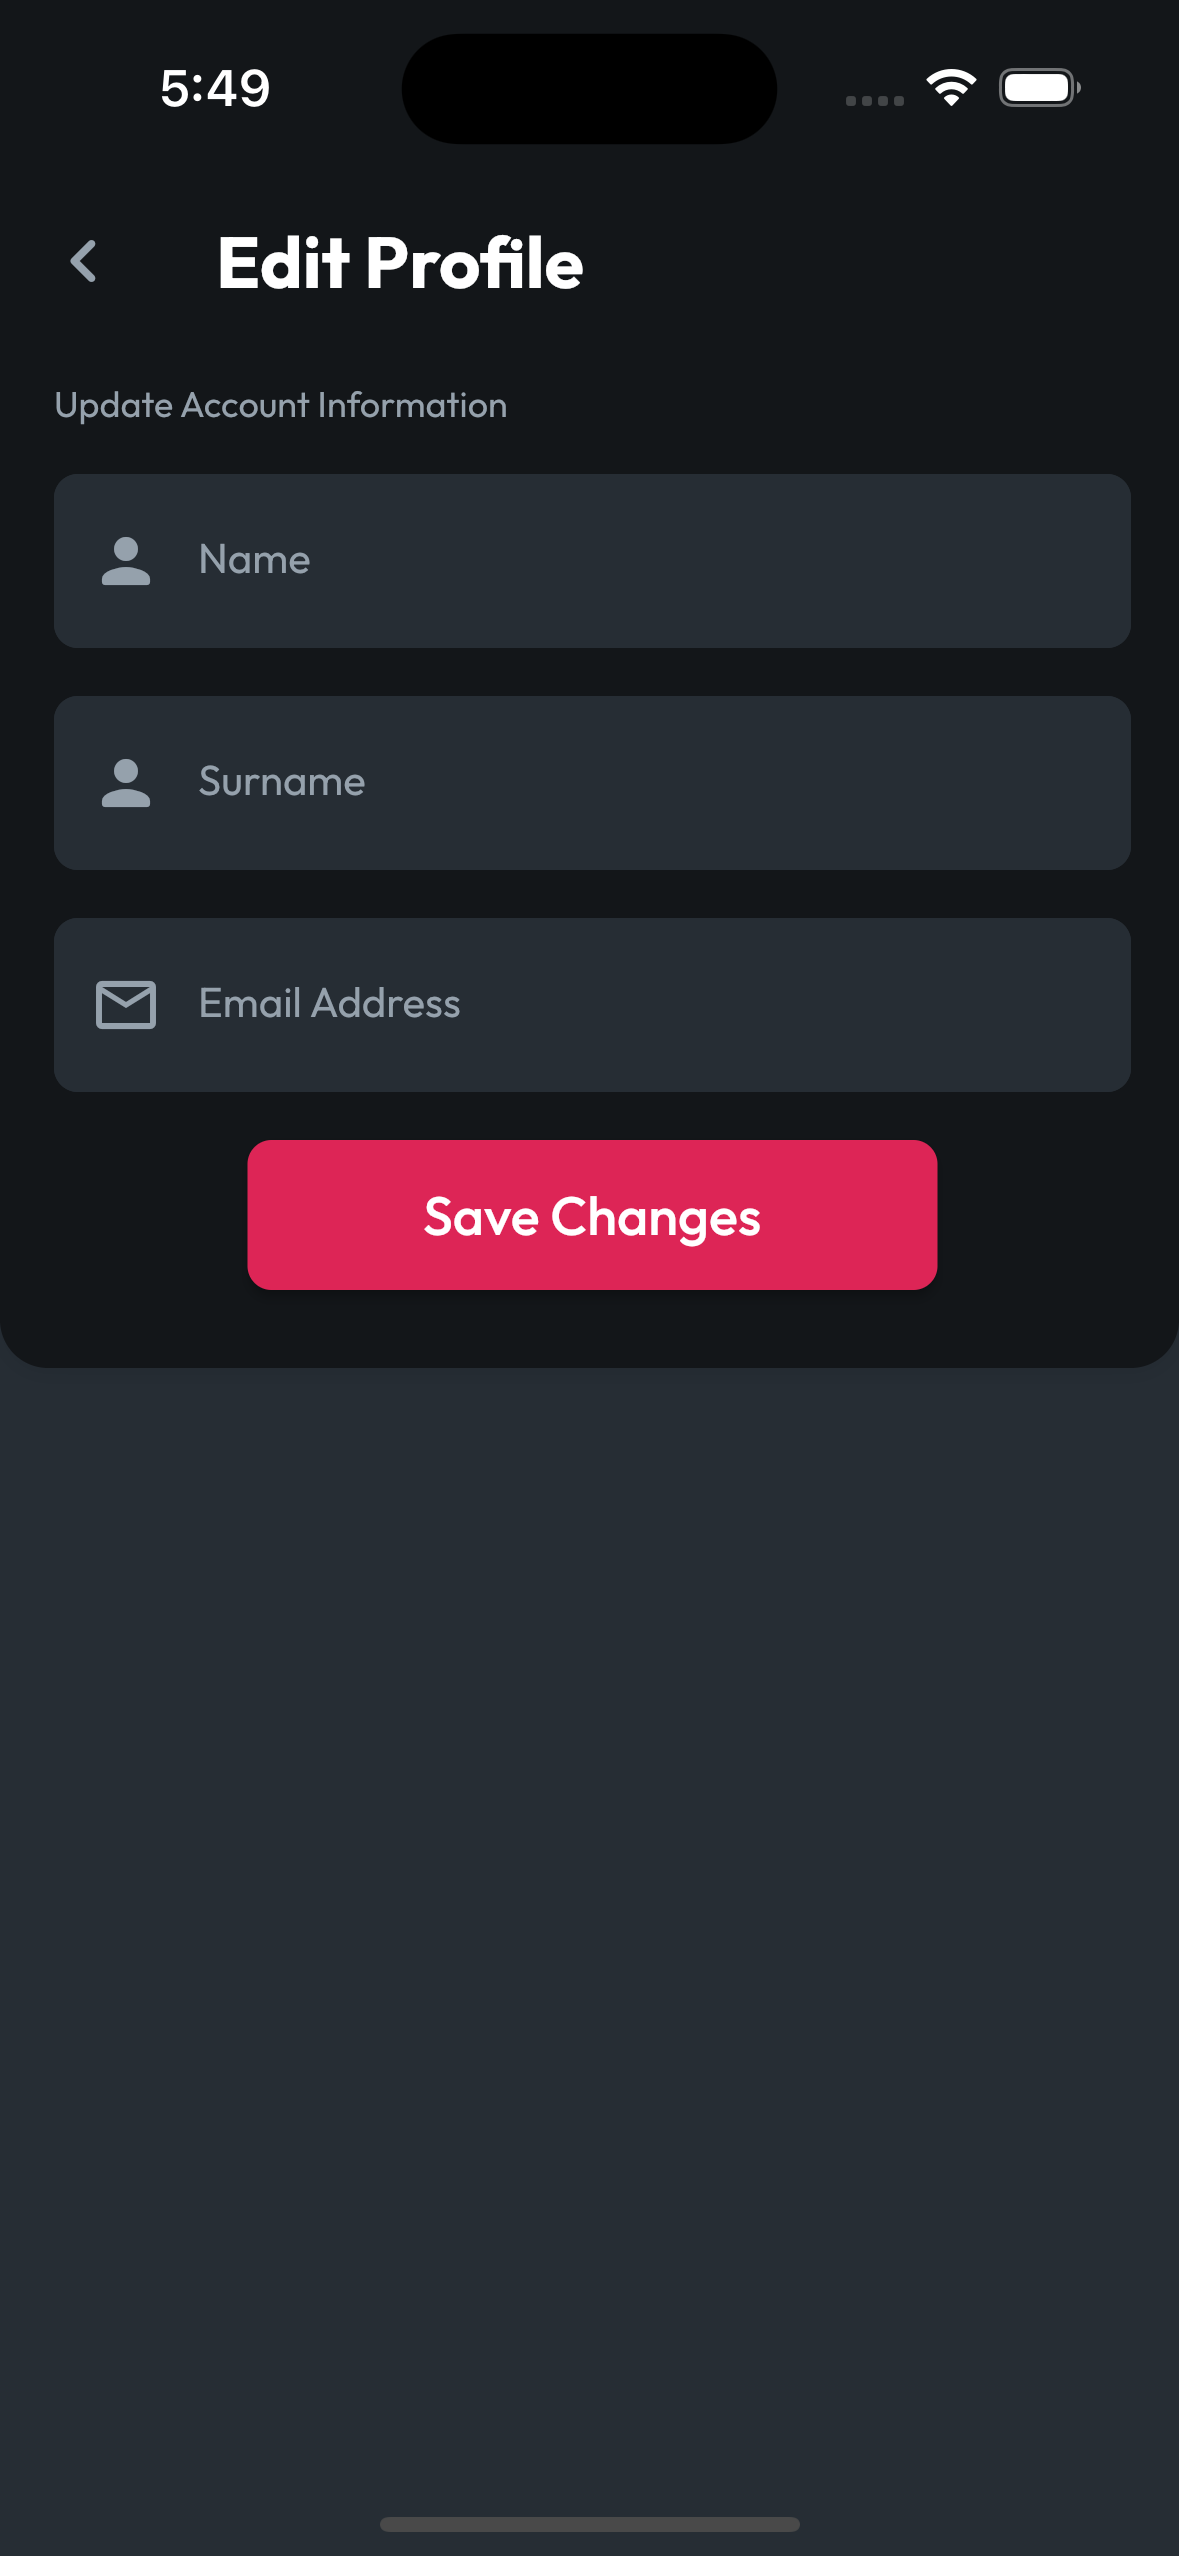
\includegraphics[scale=0.1]{Images/Screenshots/Mobile/EditProfile.png}
  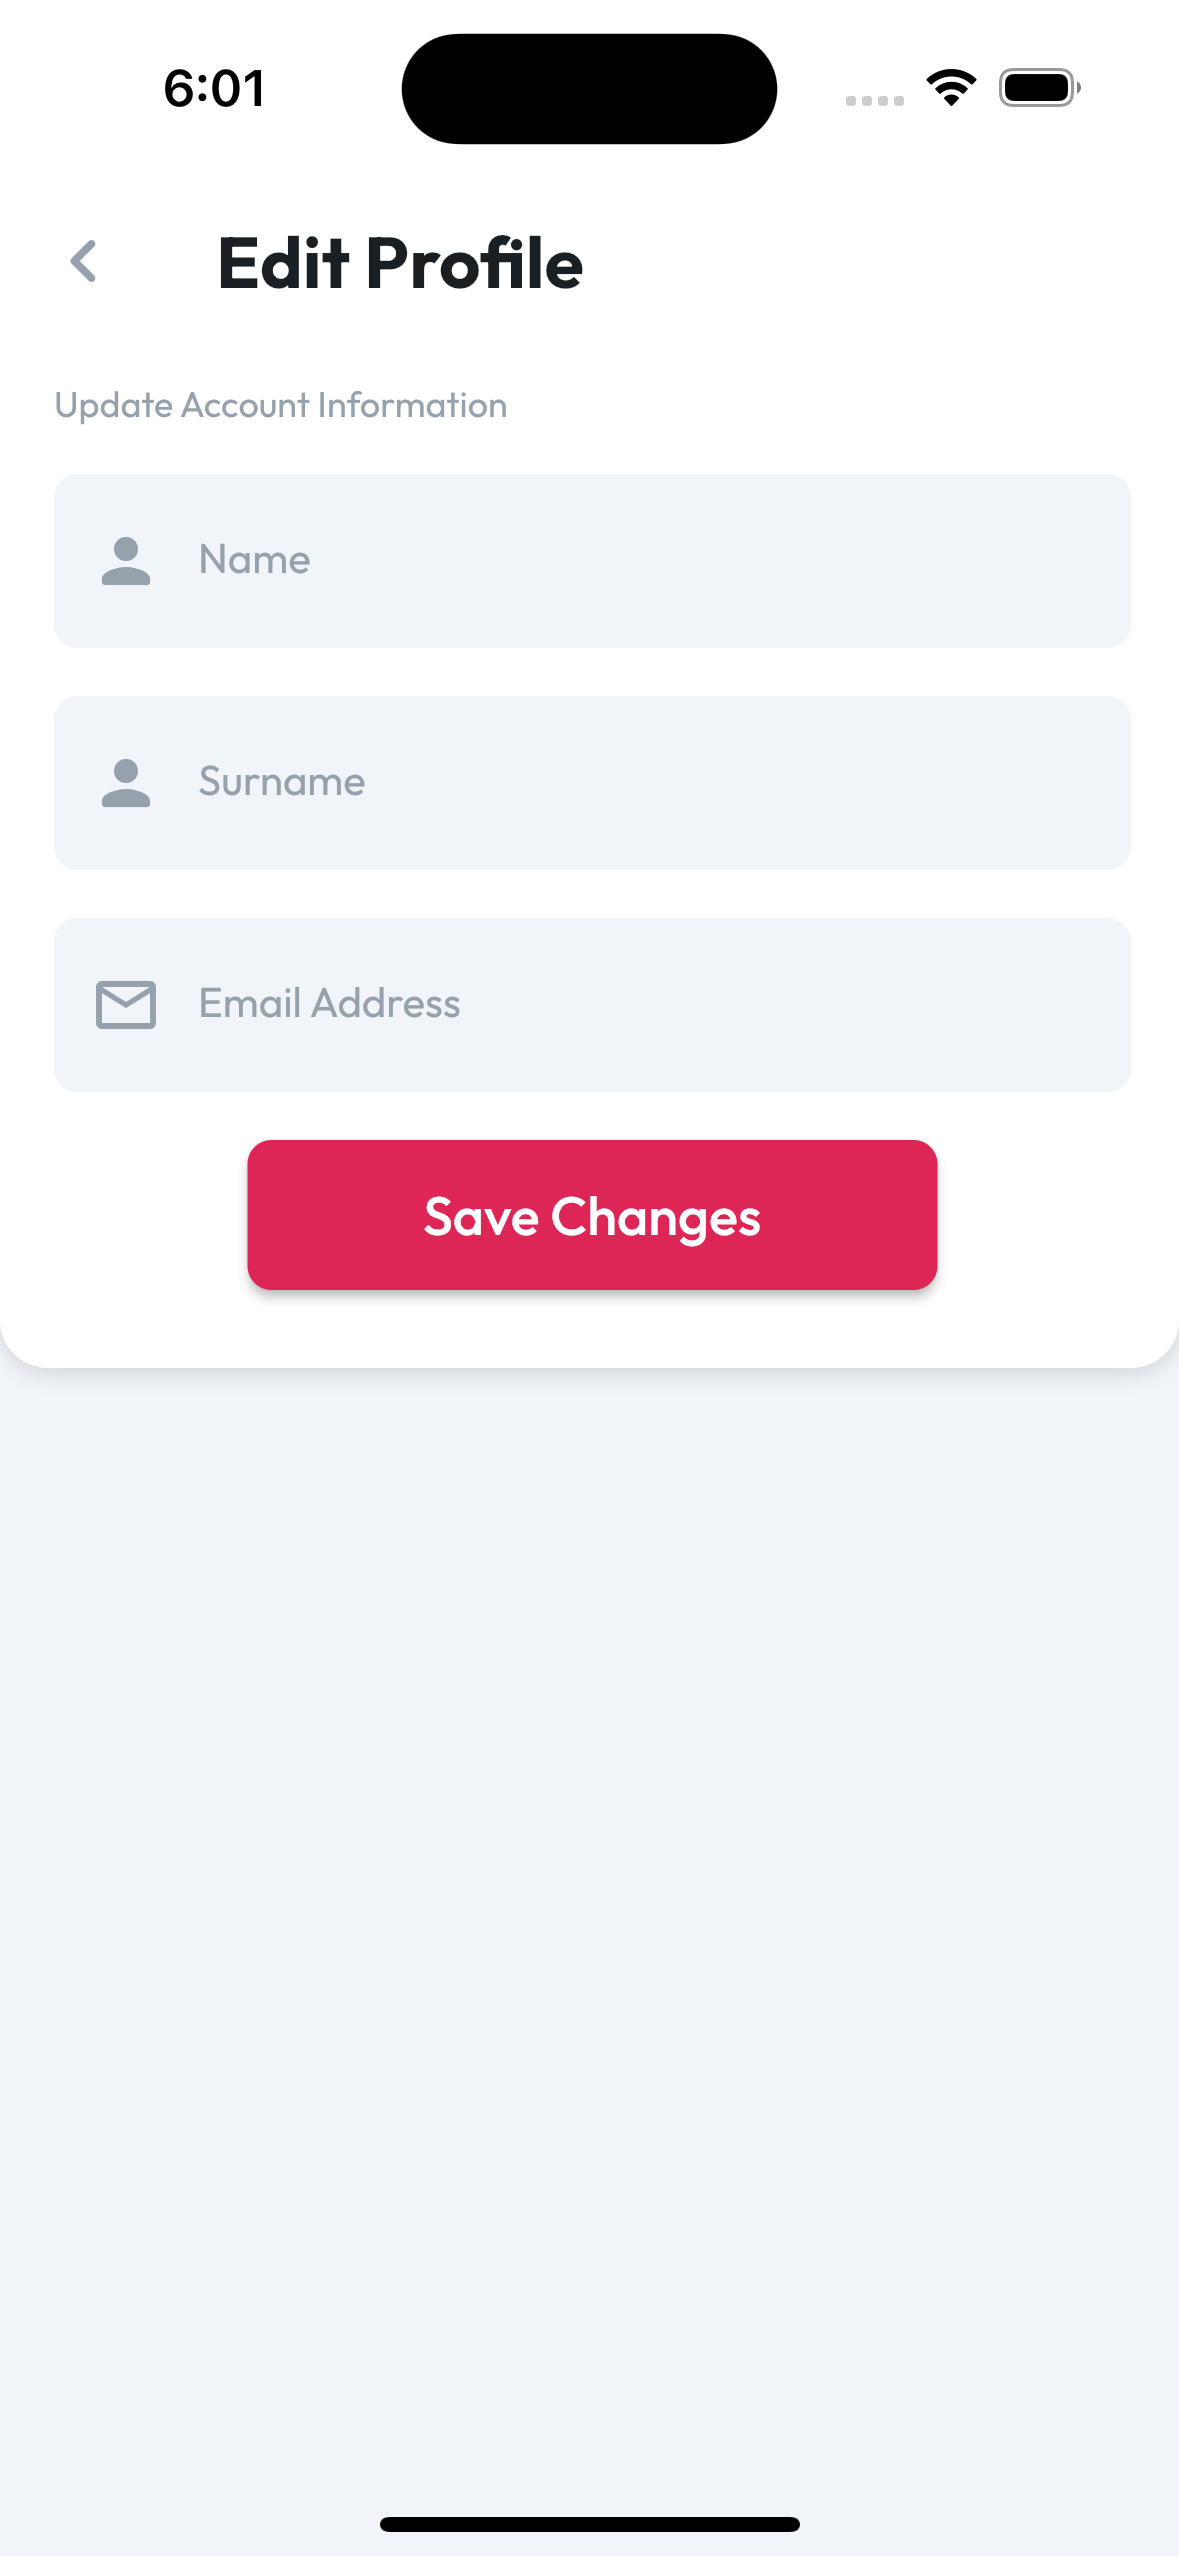
\includegraphics[scale=0.1]{Images/Screenshots/Mobile/EditProfileLight.png}
  \caption{Edit profile page}
\end{figure}

\clearpage

\subsection{Change password page}

\begin{minipage}{\linewidth}
    Form for updating the user's password.
\end{minipage}

\begin{figure}[!h]
  \centering
  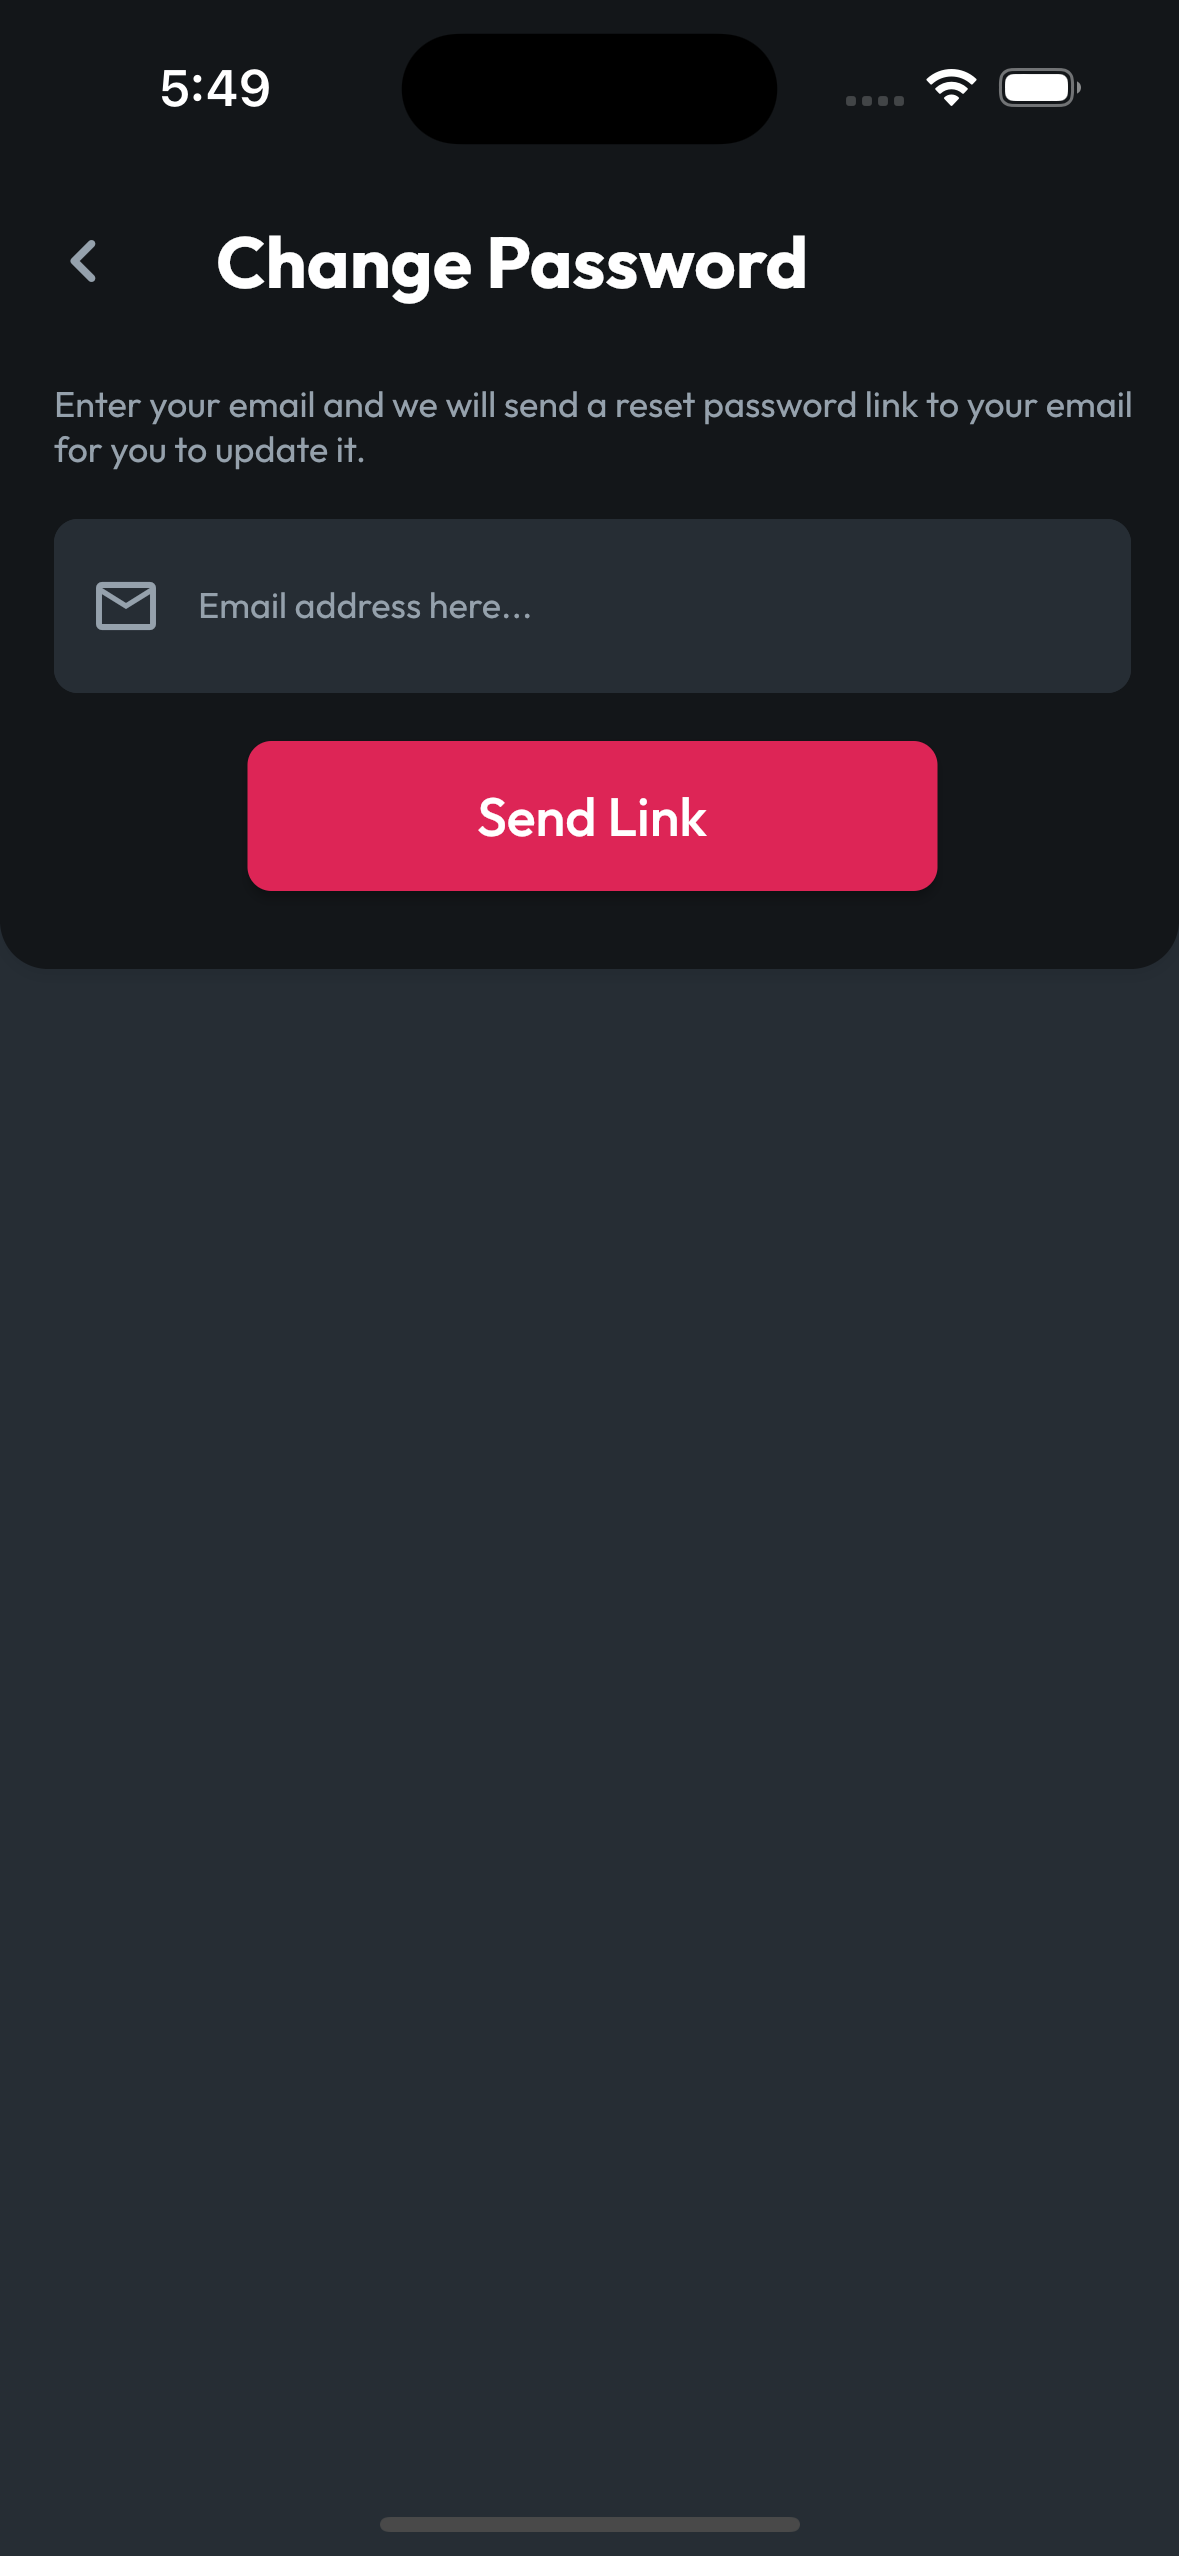
\includegraphics[scale=0.1]{Images/Screenshots/Mobile/ChangePassword.png}
  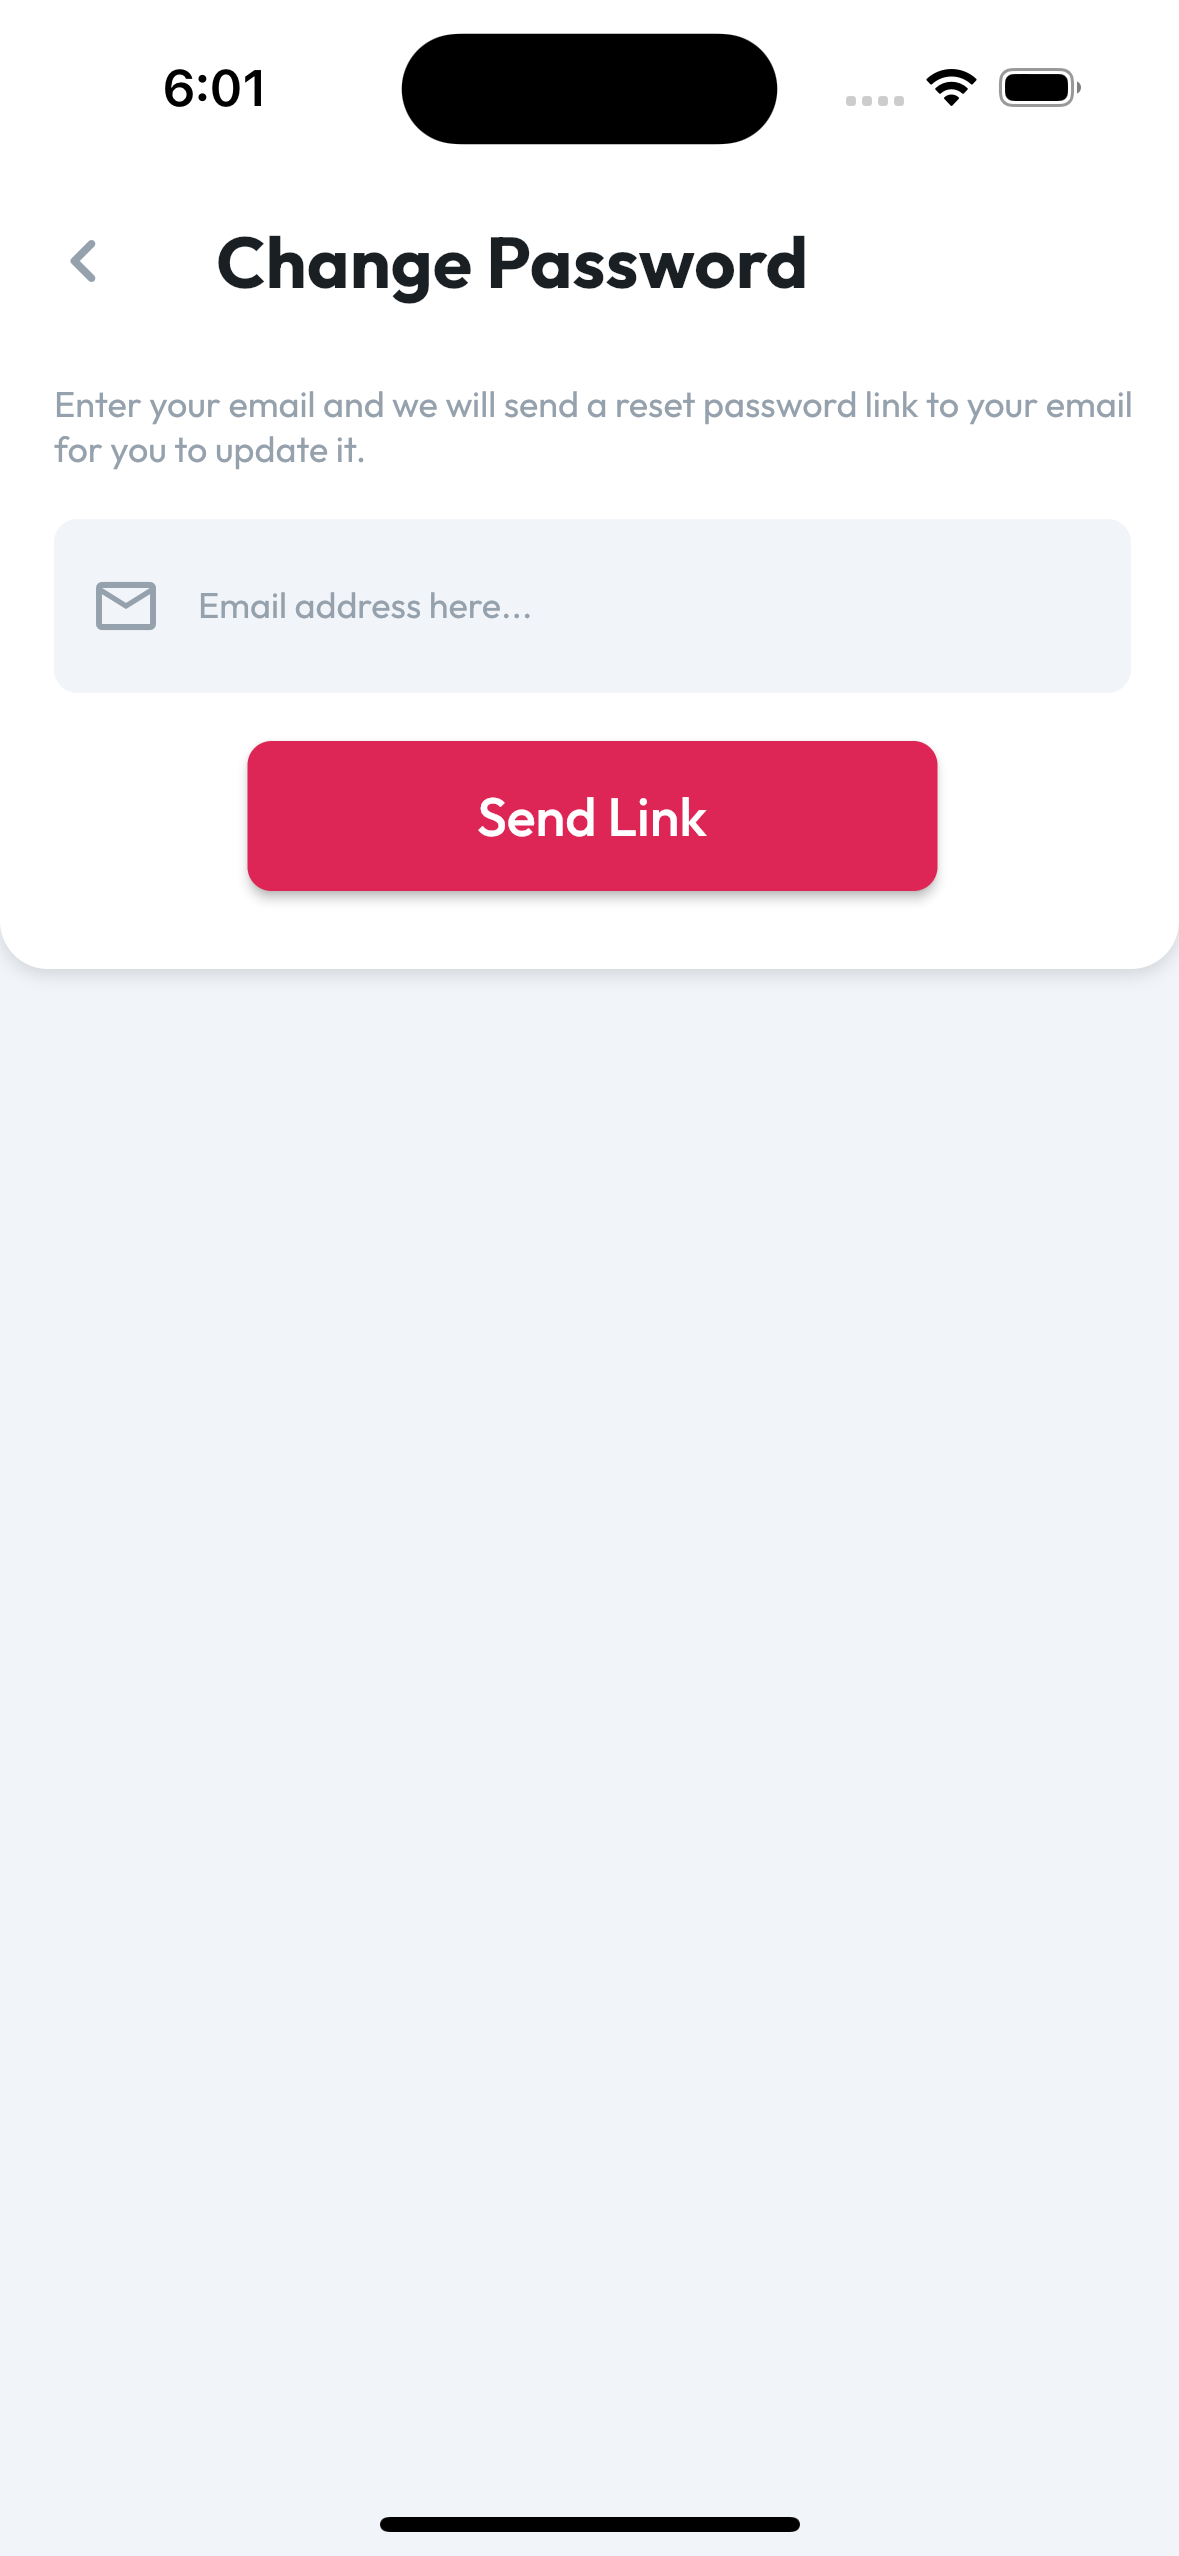
\includegraphics[scale=0.1]{Images/Screenshots/Mobile/ChangePasswordLight.png}
  \caption{Change password page}
\end{figure}

\clearpage
\section{Tablet version}
In the following sections are shown the screens of the \textbf{tablet} application.
Every page will be shown respectively in dark and light mode. \\
The content and functionalities of the pages are equals to the mobile version.

\subsection{Diary page}

\begin{figure}[!h]
  \centering
  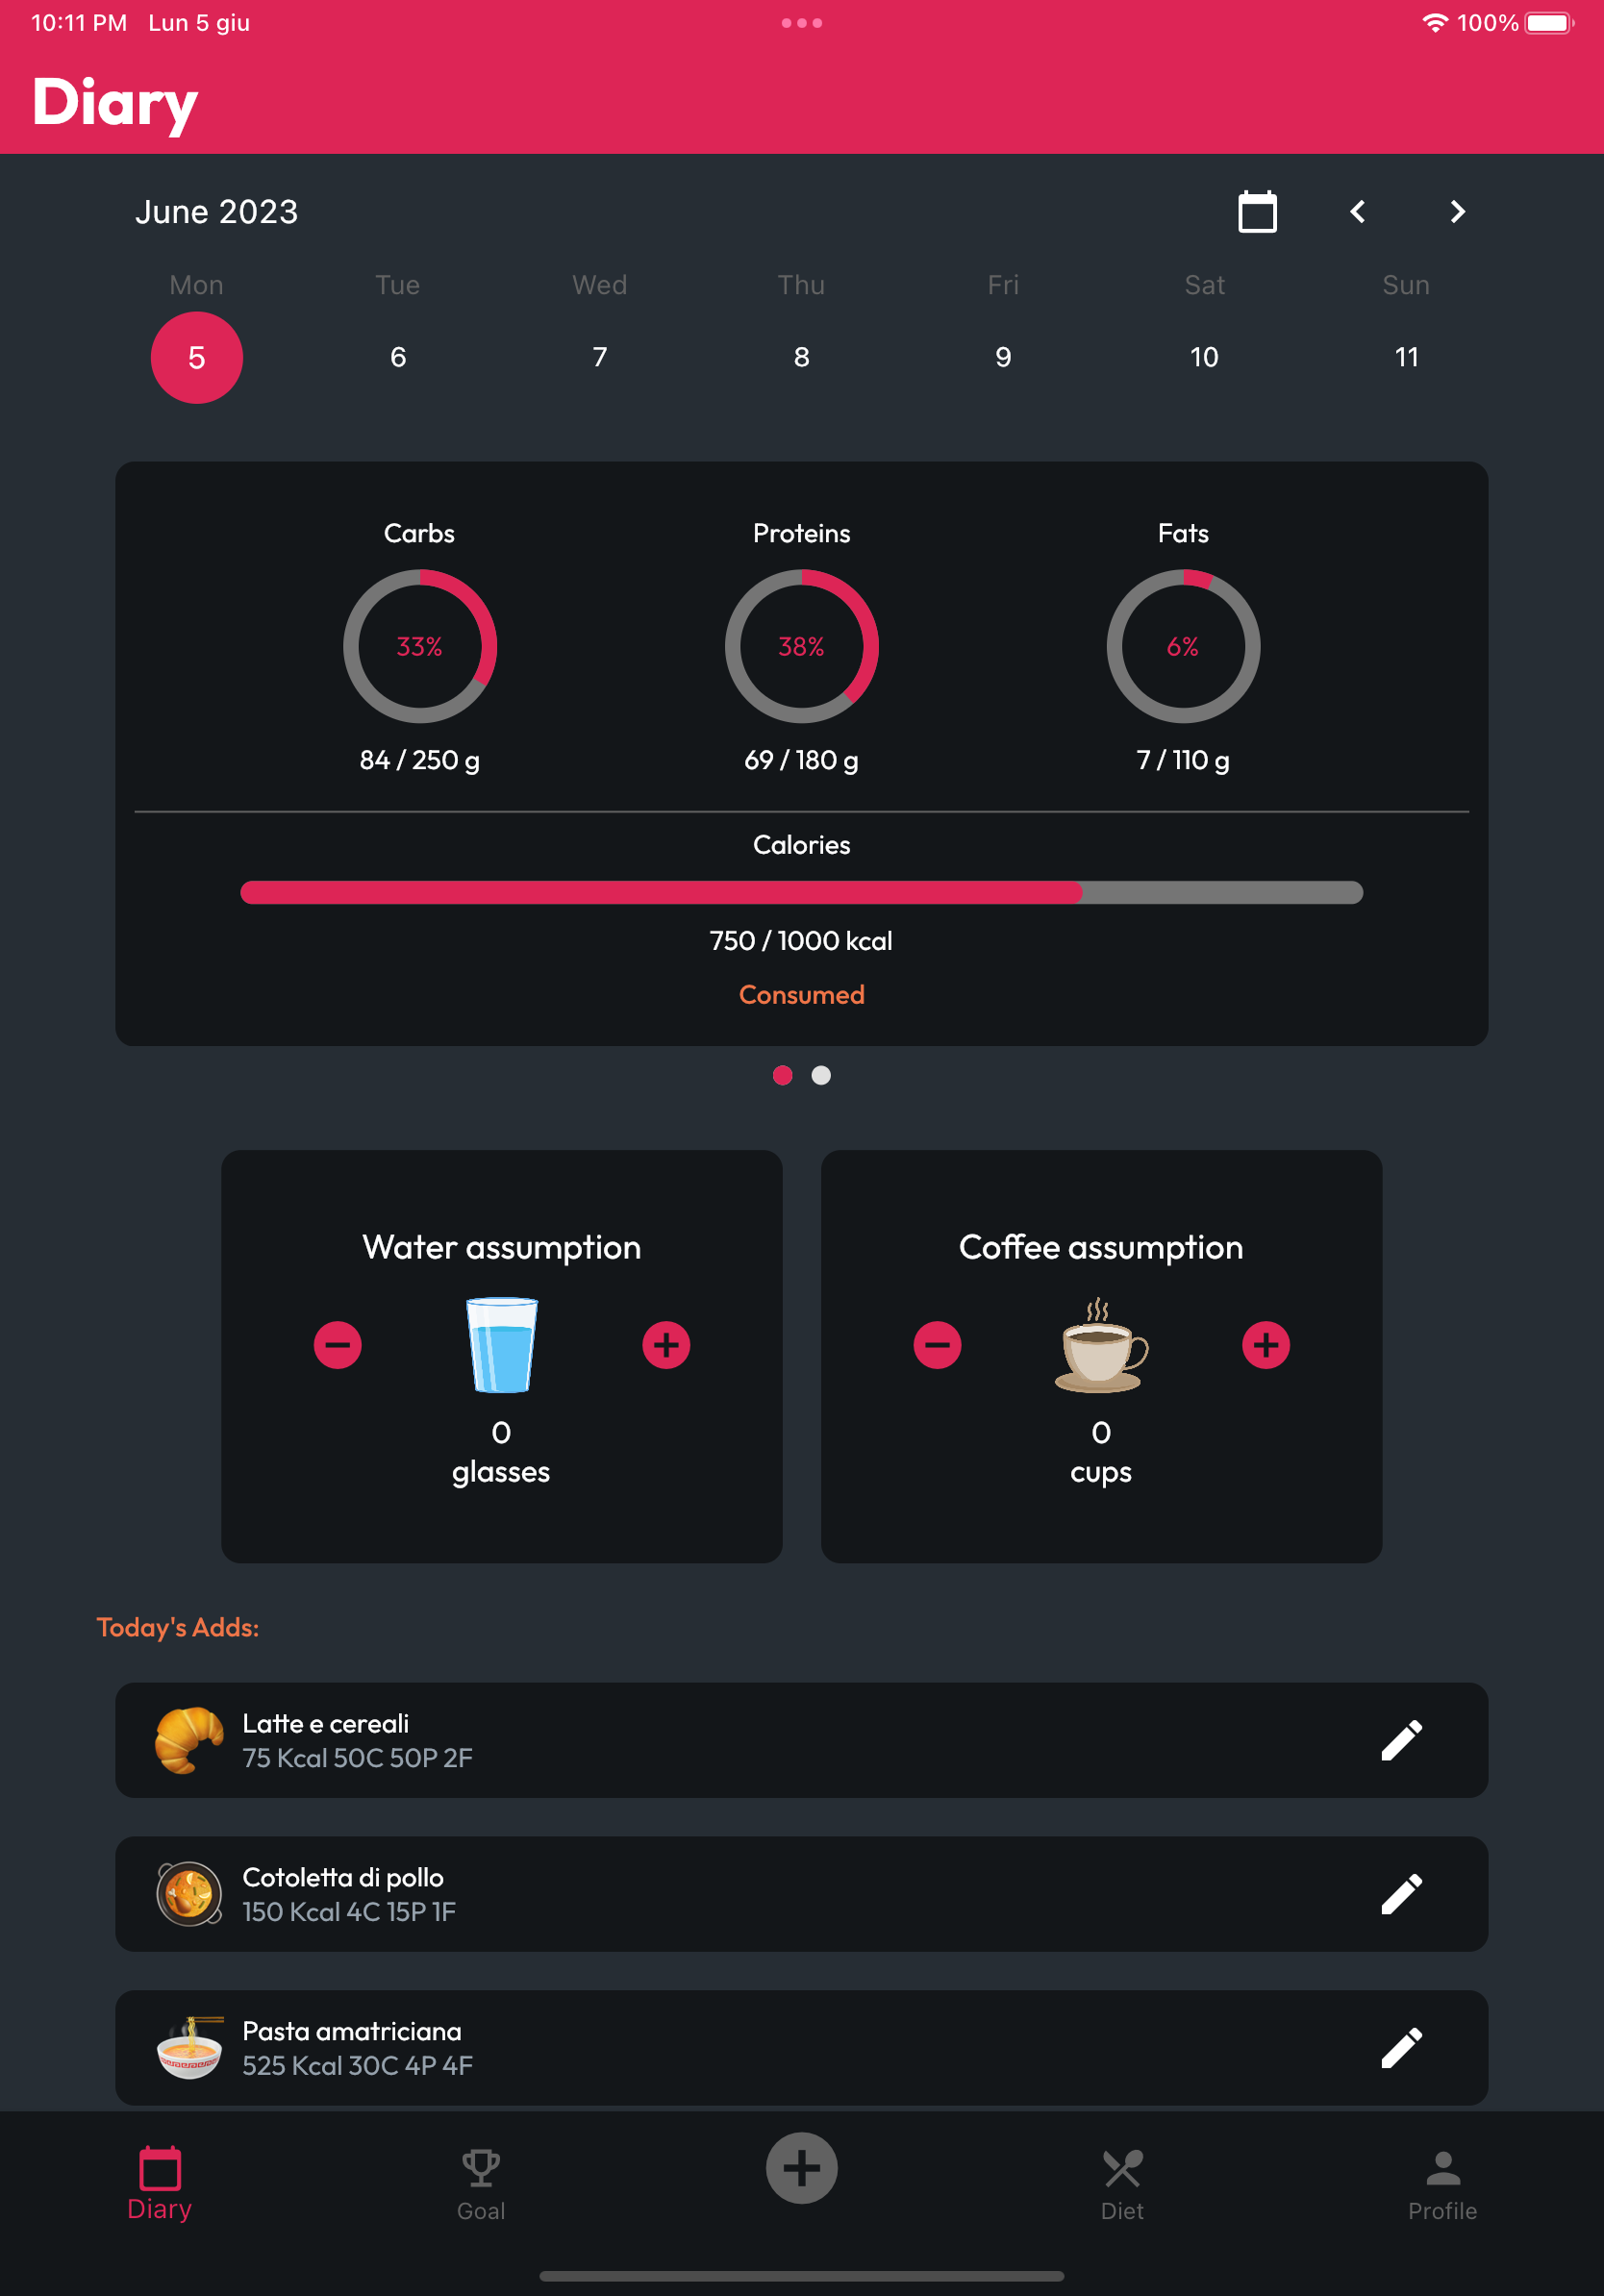
\includegraphics[scale=0.1]{Images/Screenshots/Tablet/DiaryTablet.png}
  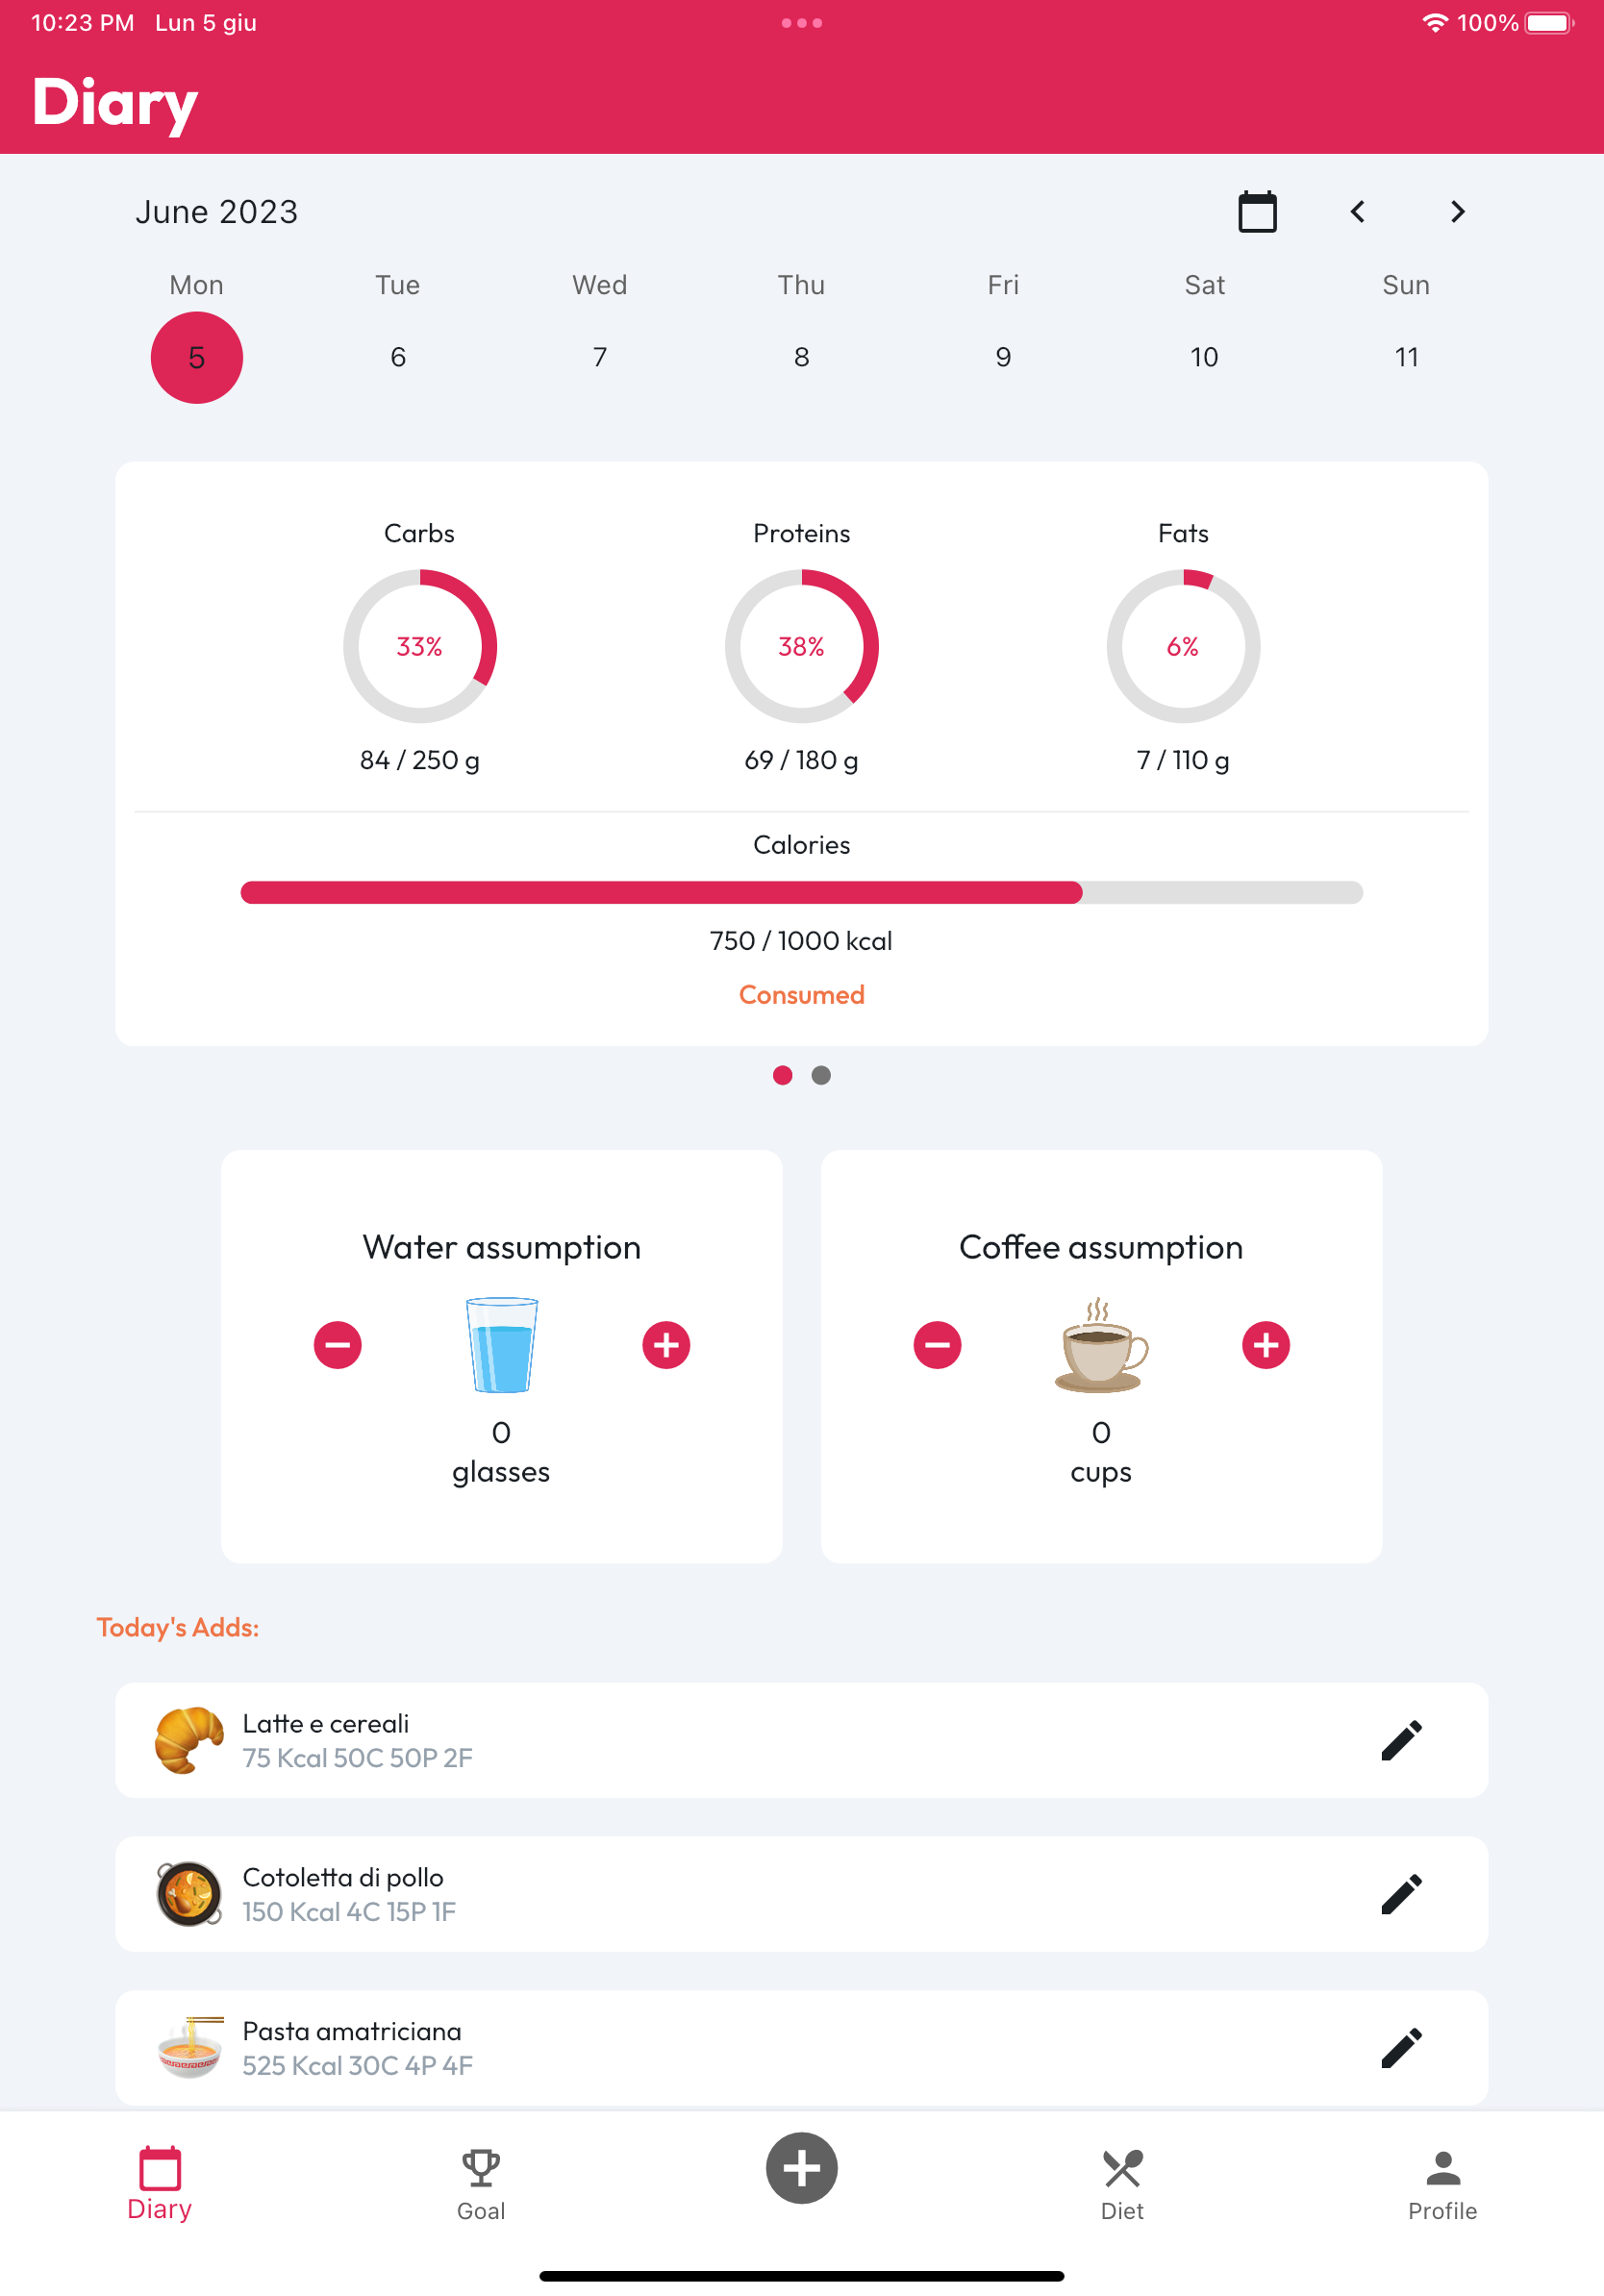
\includegraphics[scale=0.1]{Images/Screenshots/Tablet/DiaryTabletLight.png}
  \caption{Diary tablet page}
\end{figure}

\clearpage

\subsection{Edit food page}

\begin{figure}[!h]
  \centering
  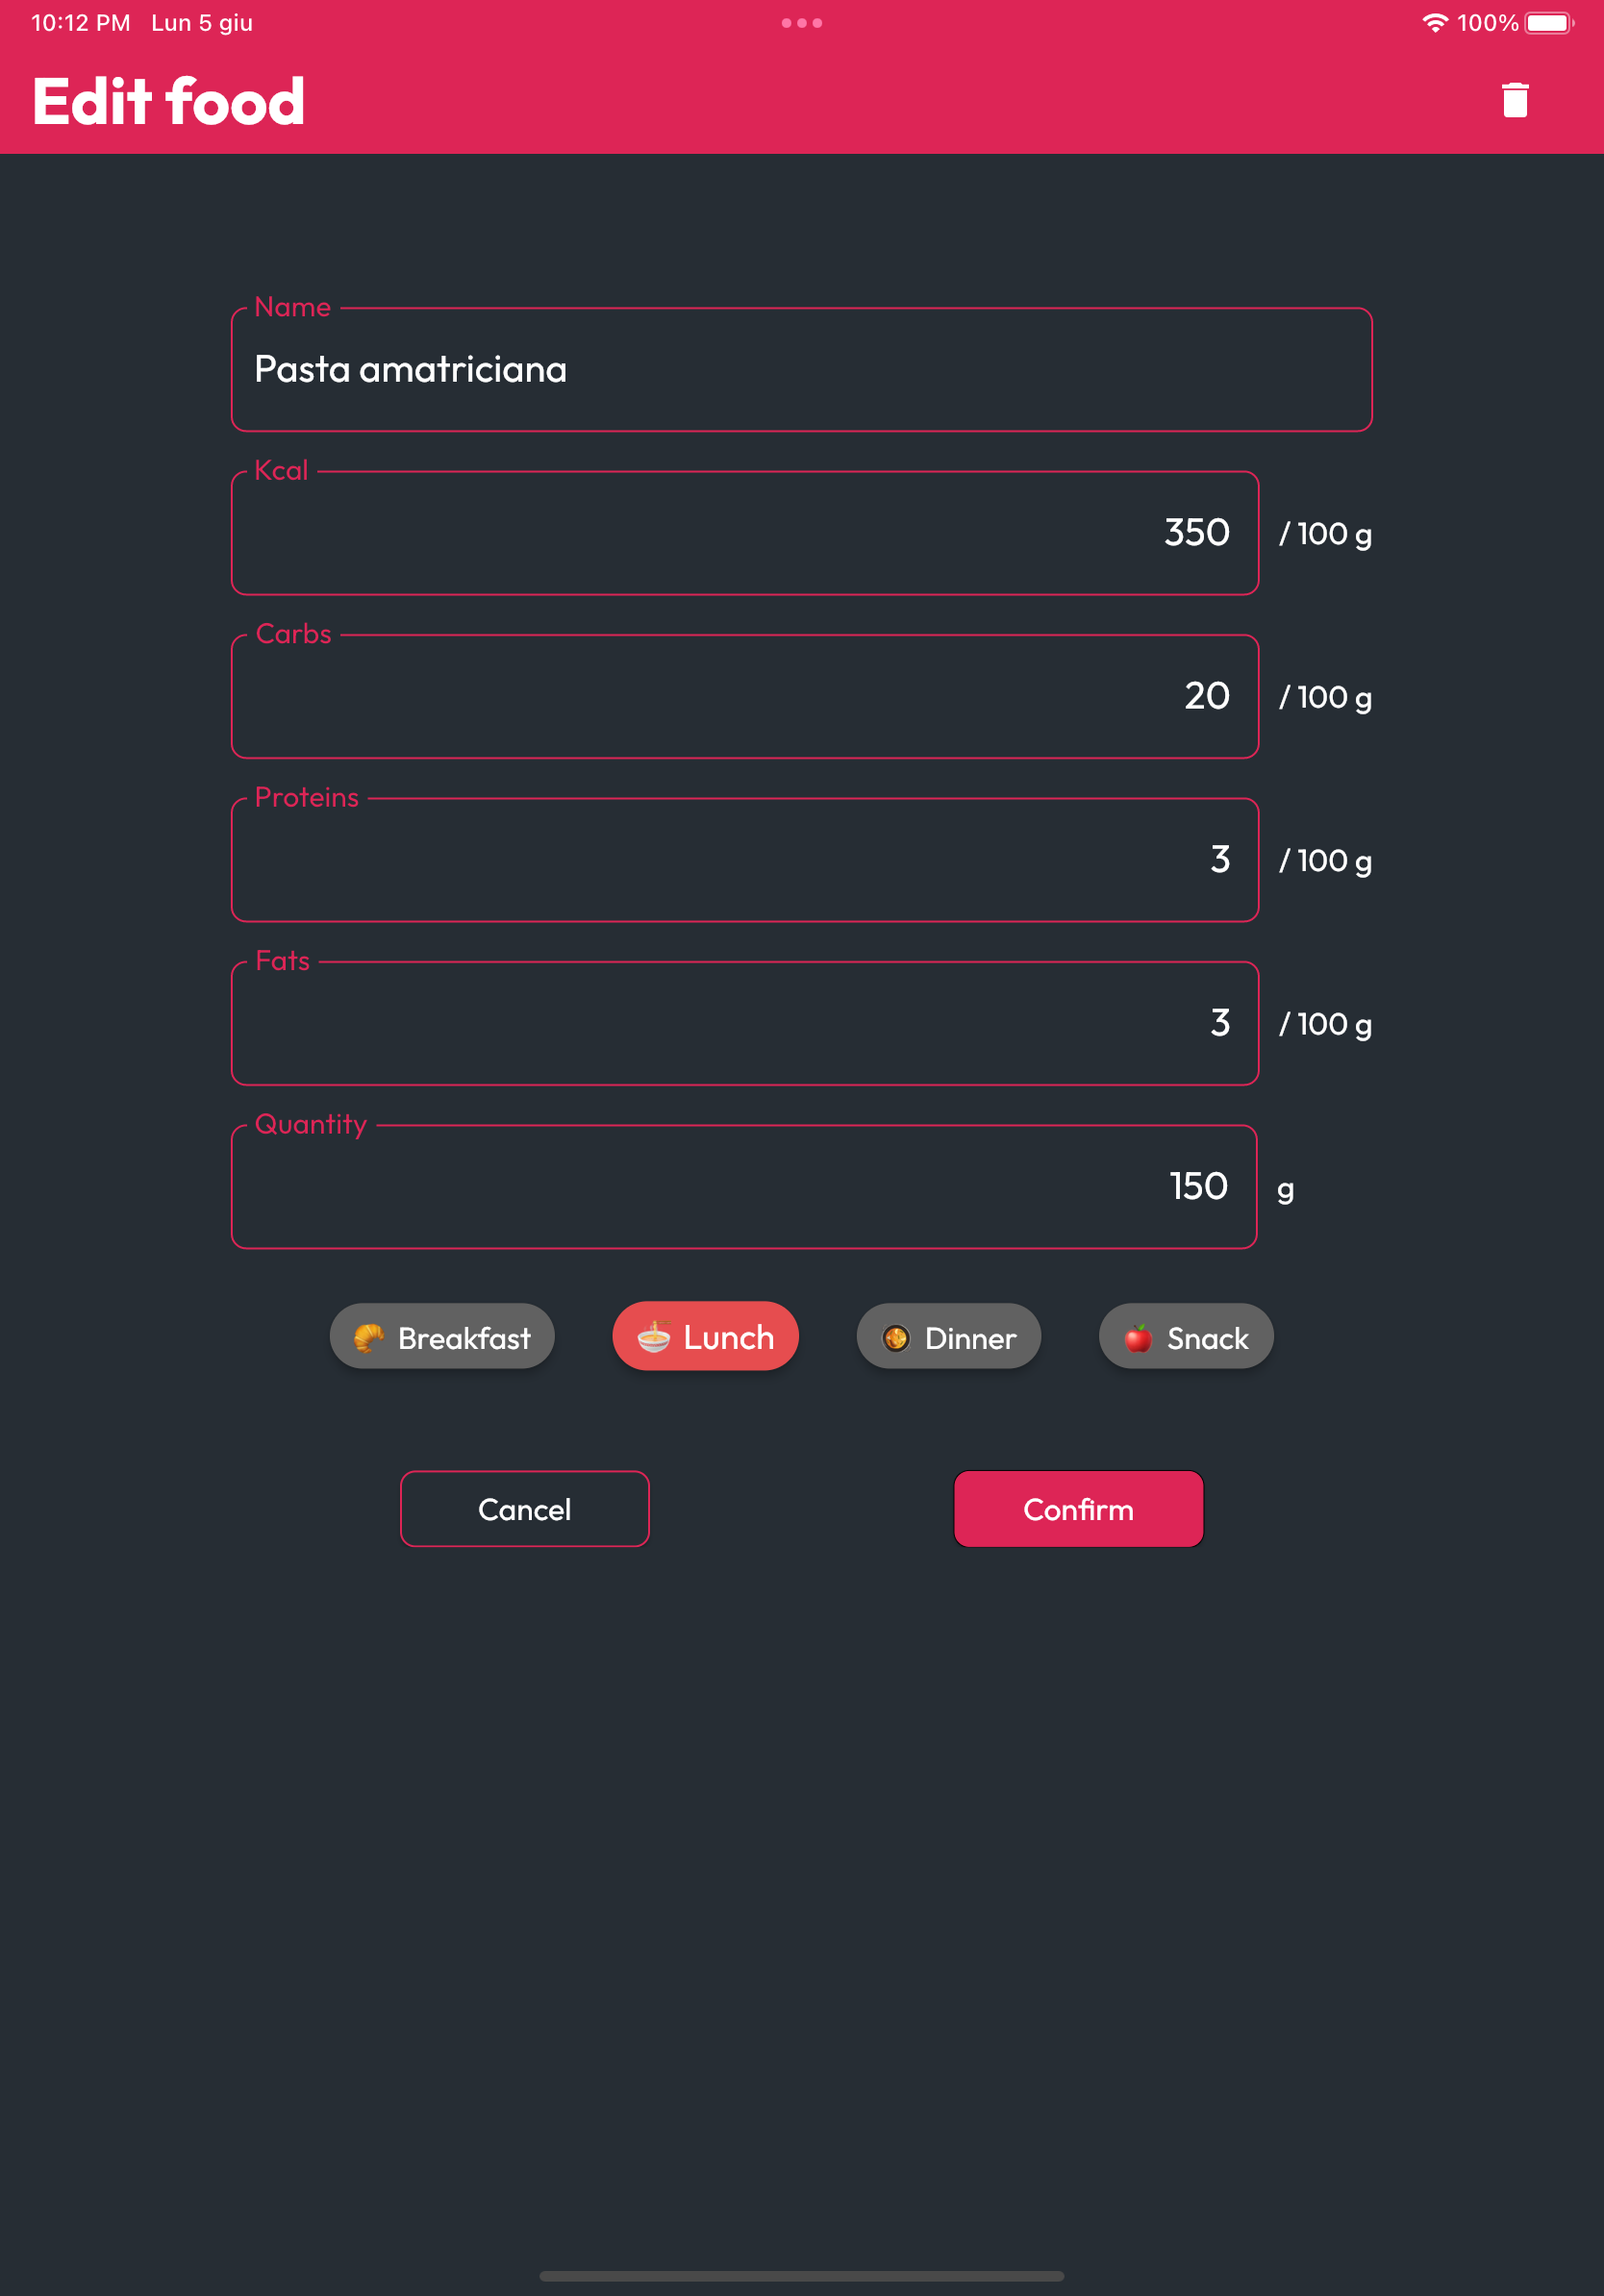
\includegraphics[scale=0.1]{Images/Screenshots/Tablet/EditFoodTablet.png}
  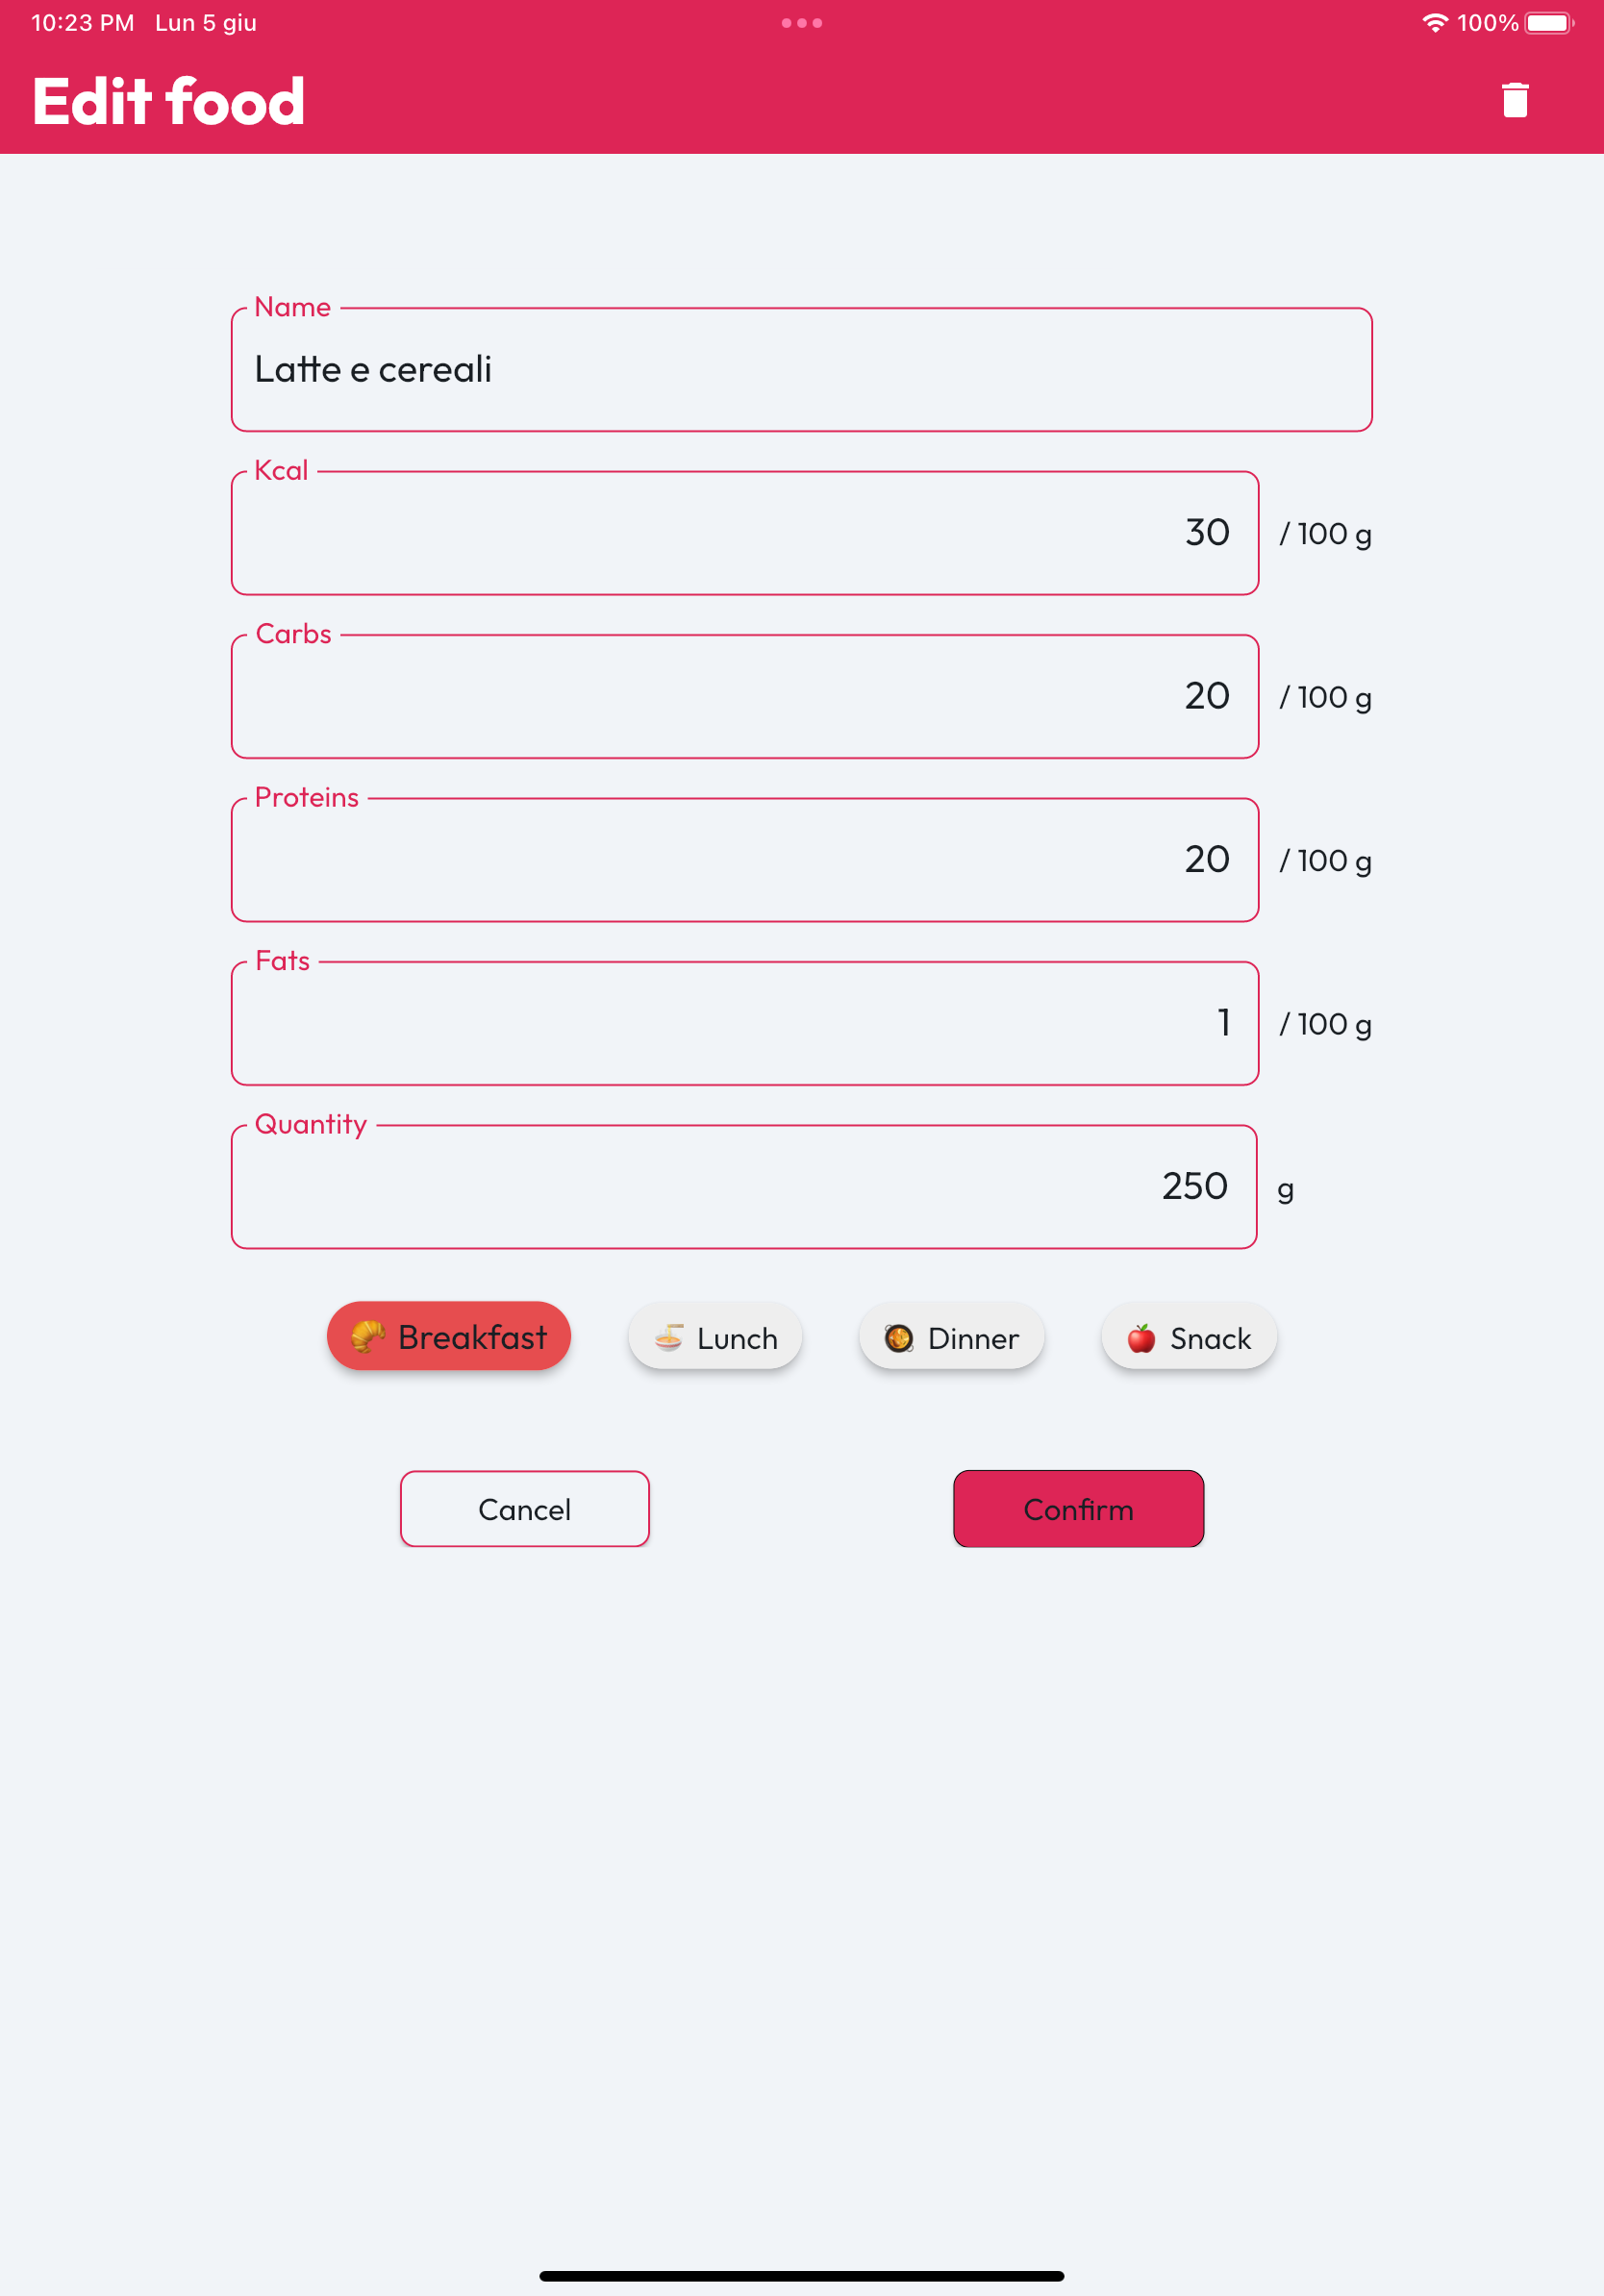
\includegraphics[scale=0.1]{Images/Screenshots/Tablet/EditFoodTabletLight.png}
  \caption{Edit food tablet page}
\end{figure}

\clearpage

\subsection{Goal page}

\begin{figure}[!h]
  \centering
  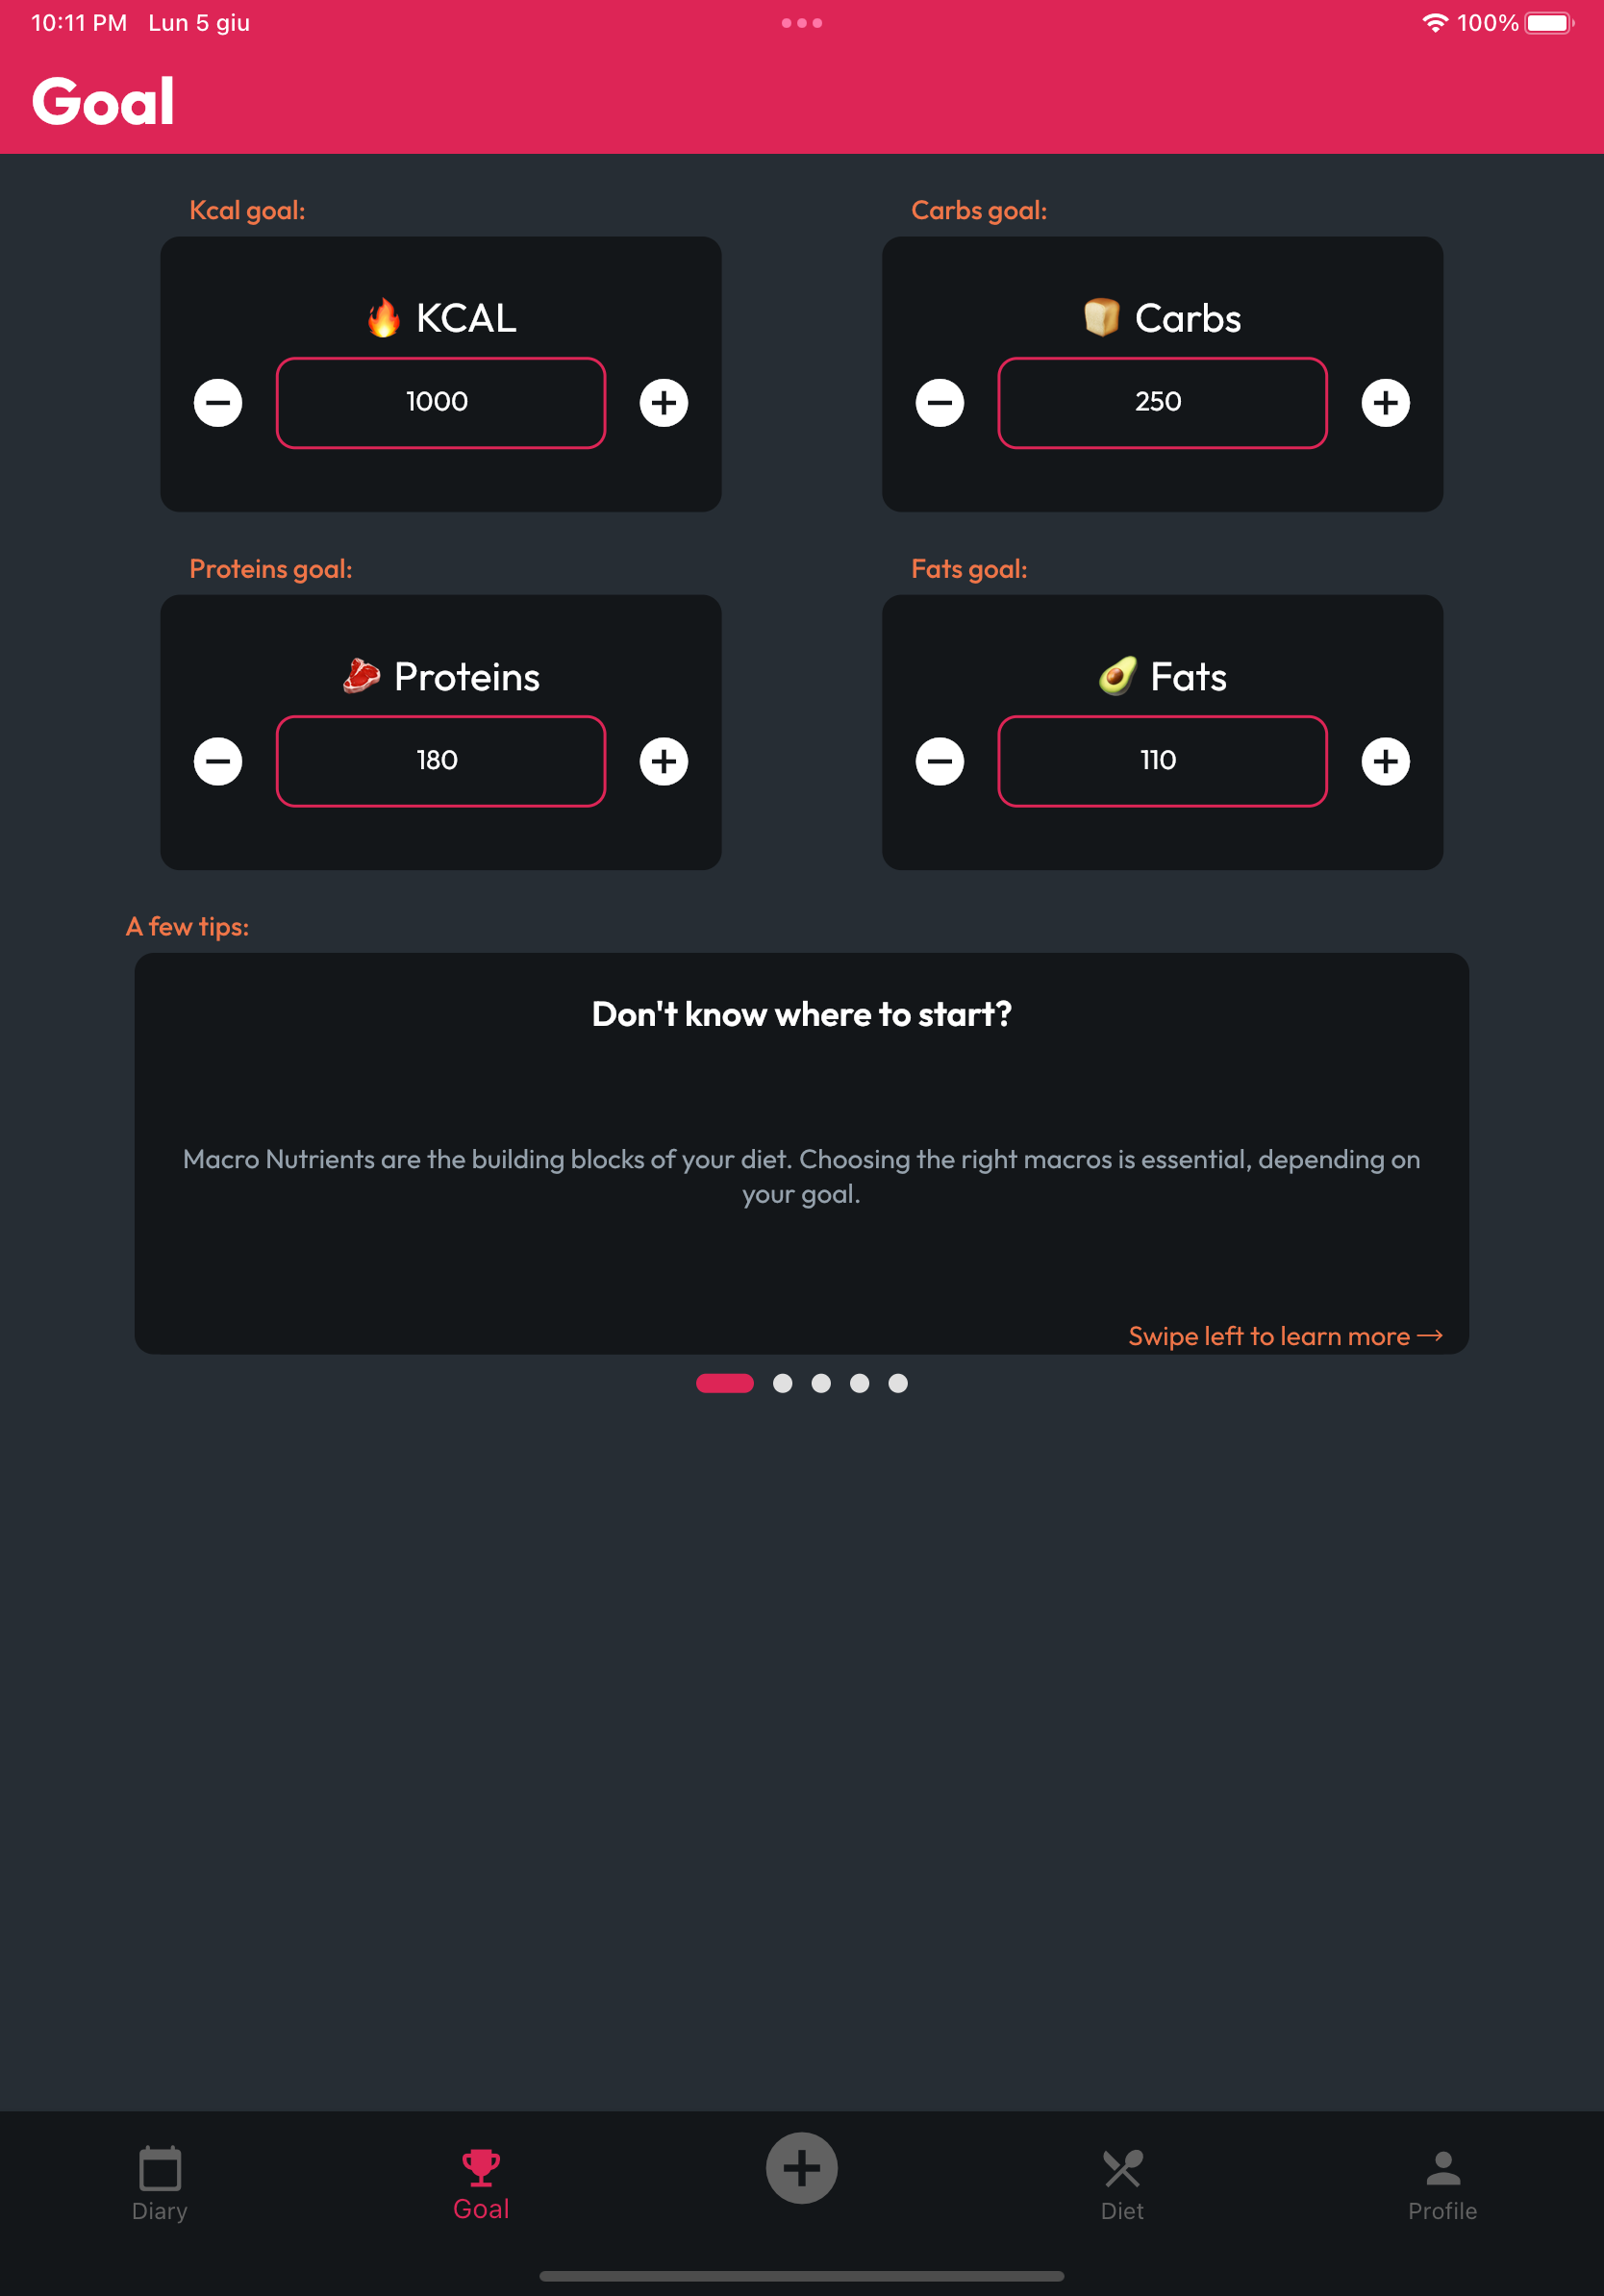
\includegraphics[scale=0.1]{Images/Screenshots/Tablet/GoalTablet.png}
  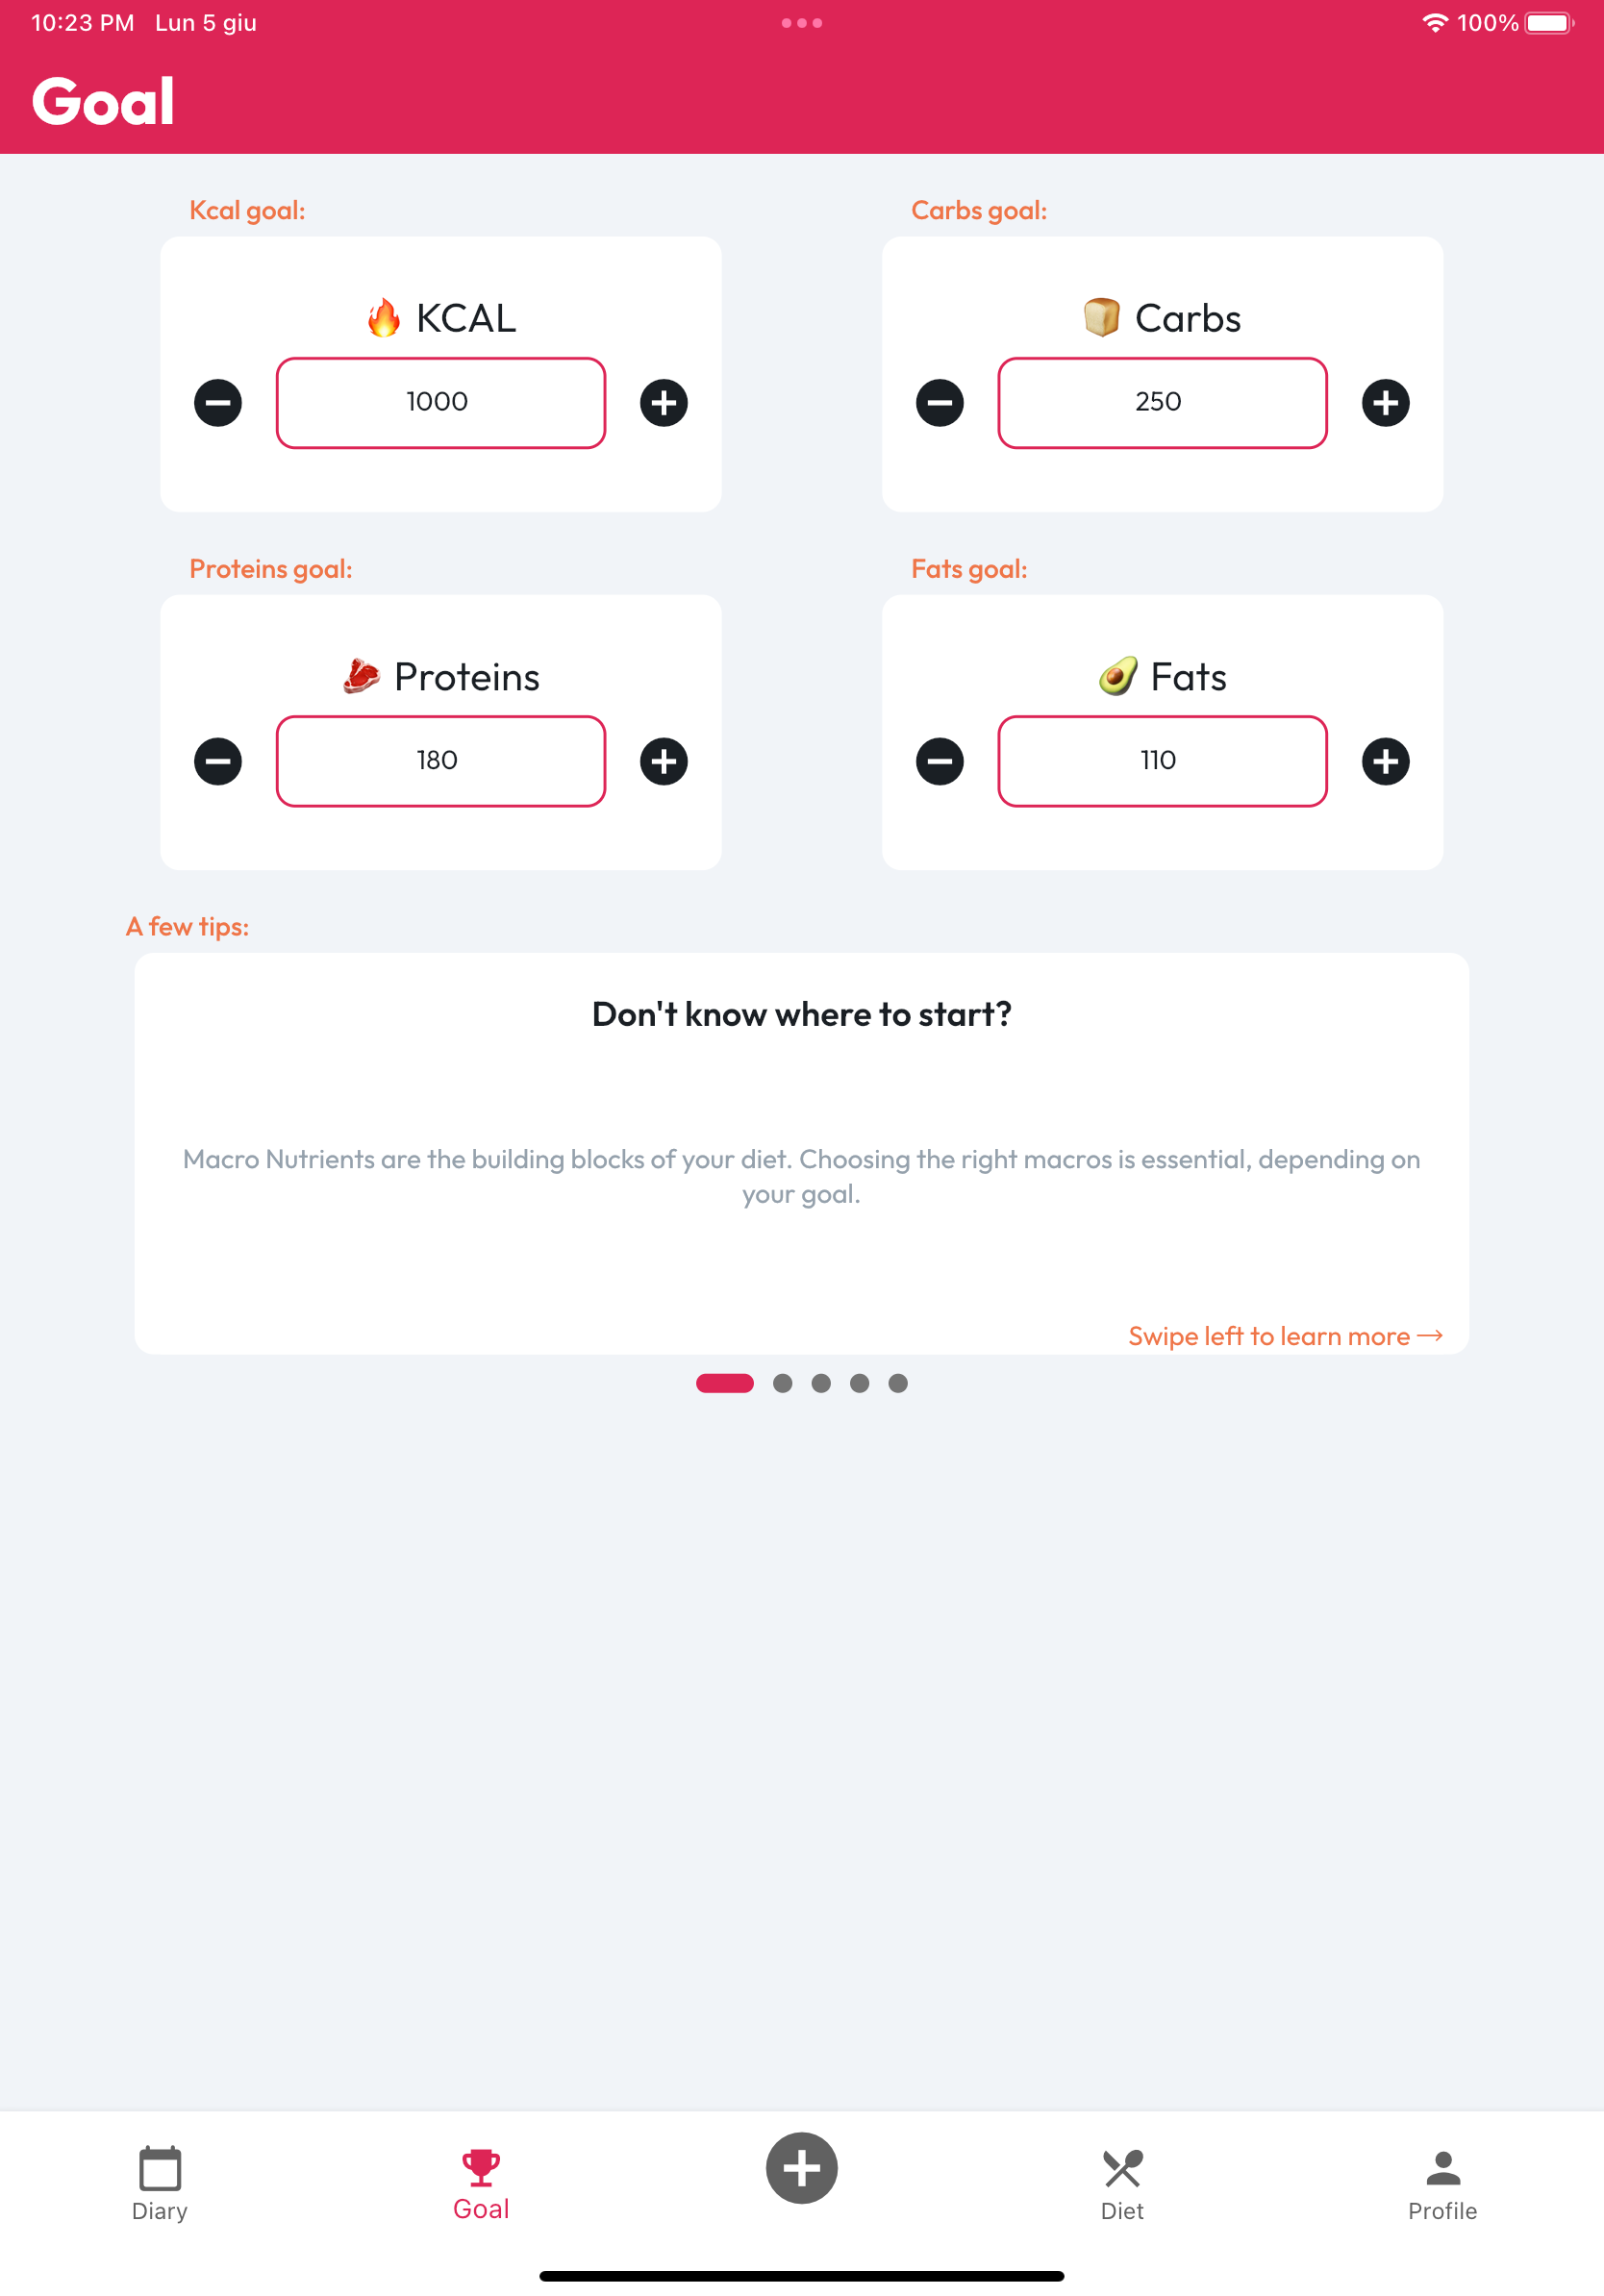
\includegraphics[scale=0.1]{Images/Screenshots/Tablet/GoalTabletLight.png}
  \caption{Goal tablet page}
\end{figure}

\clearpage

\subsection{Add page}

\begin{figure}[!h]
  \centering
  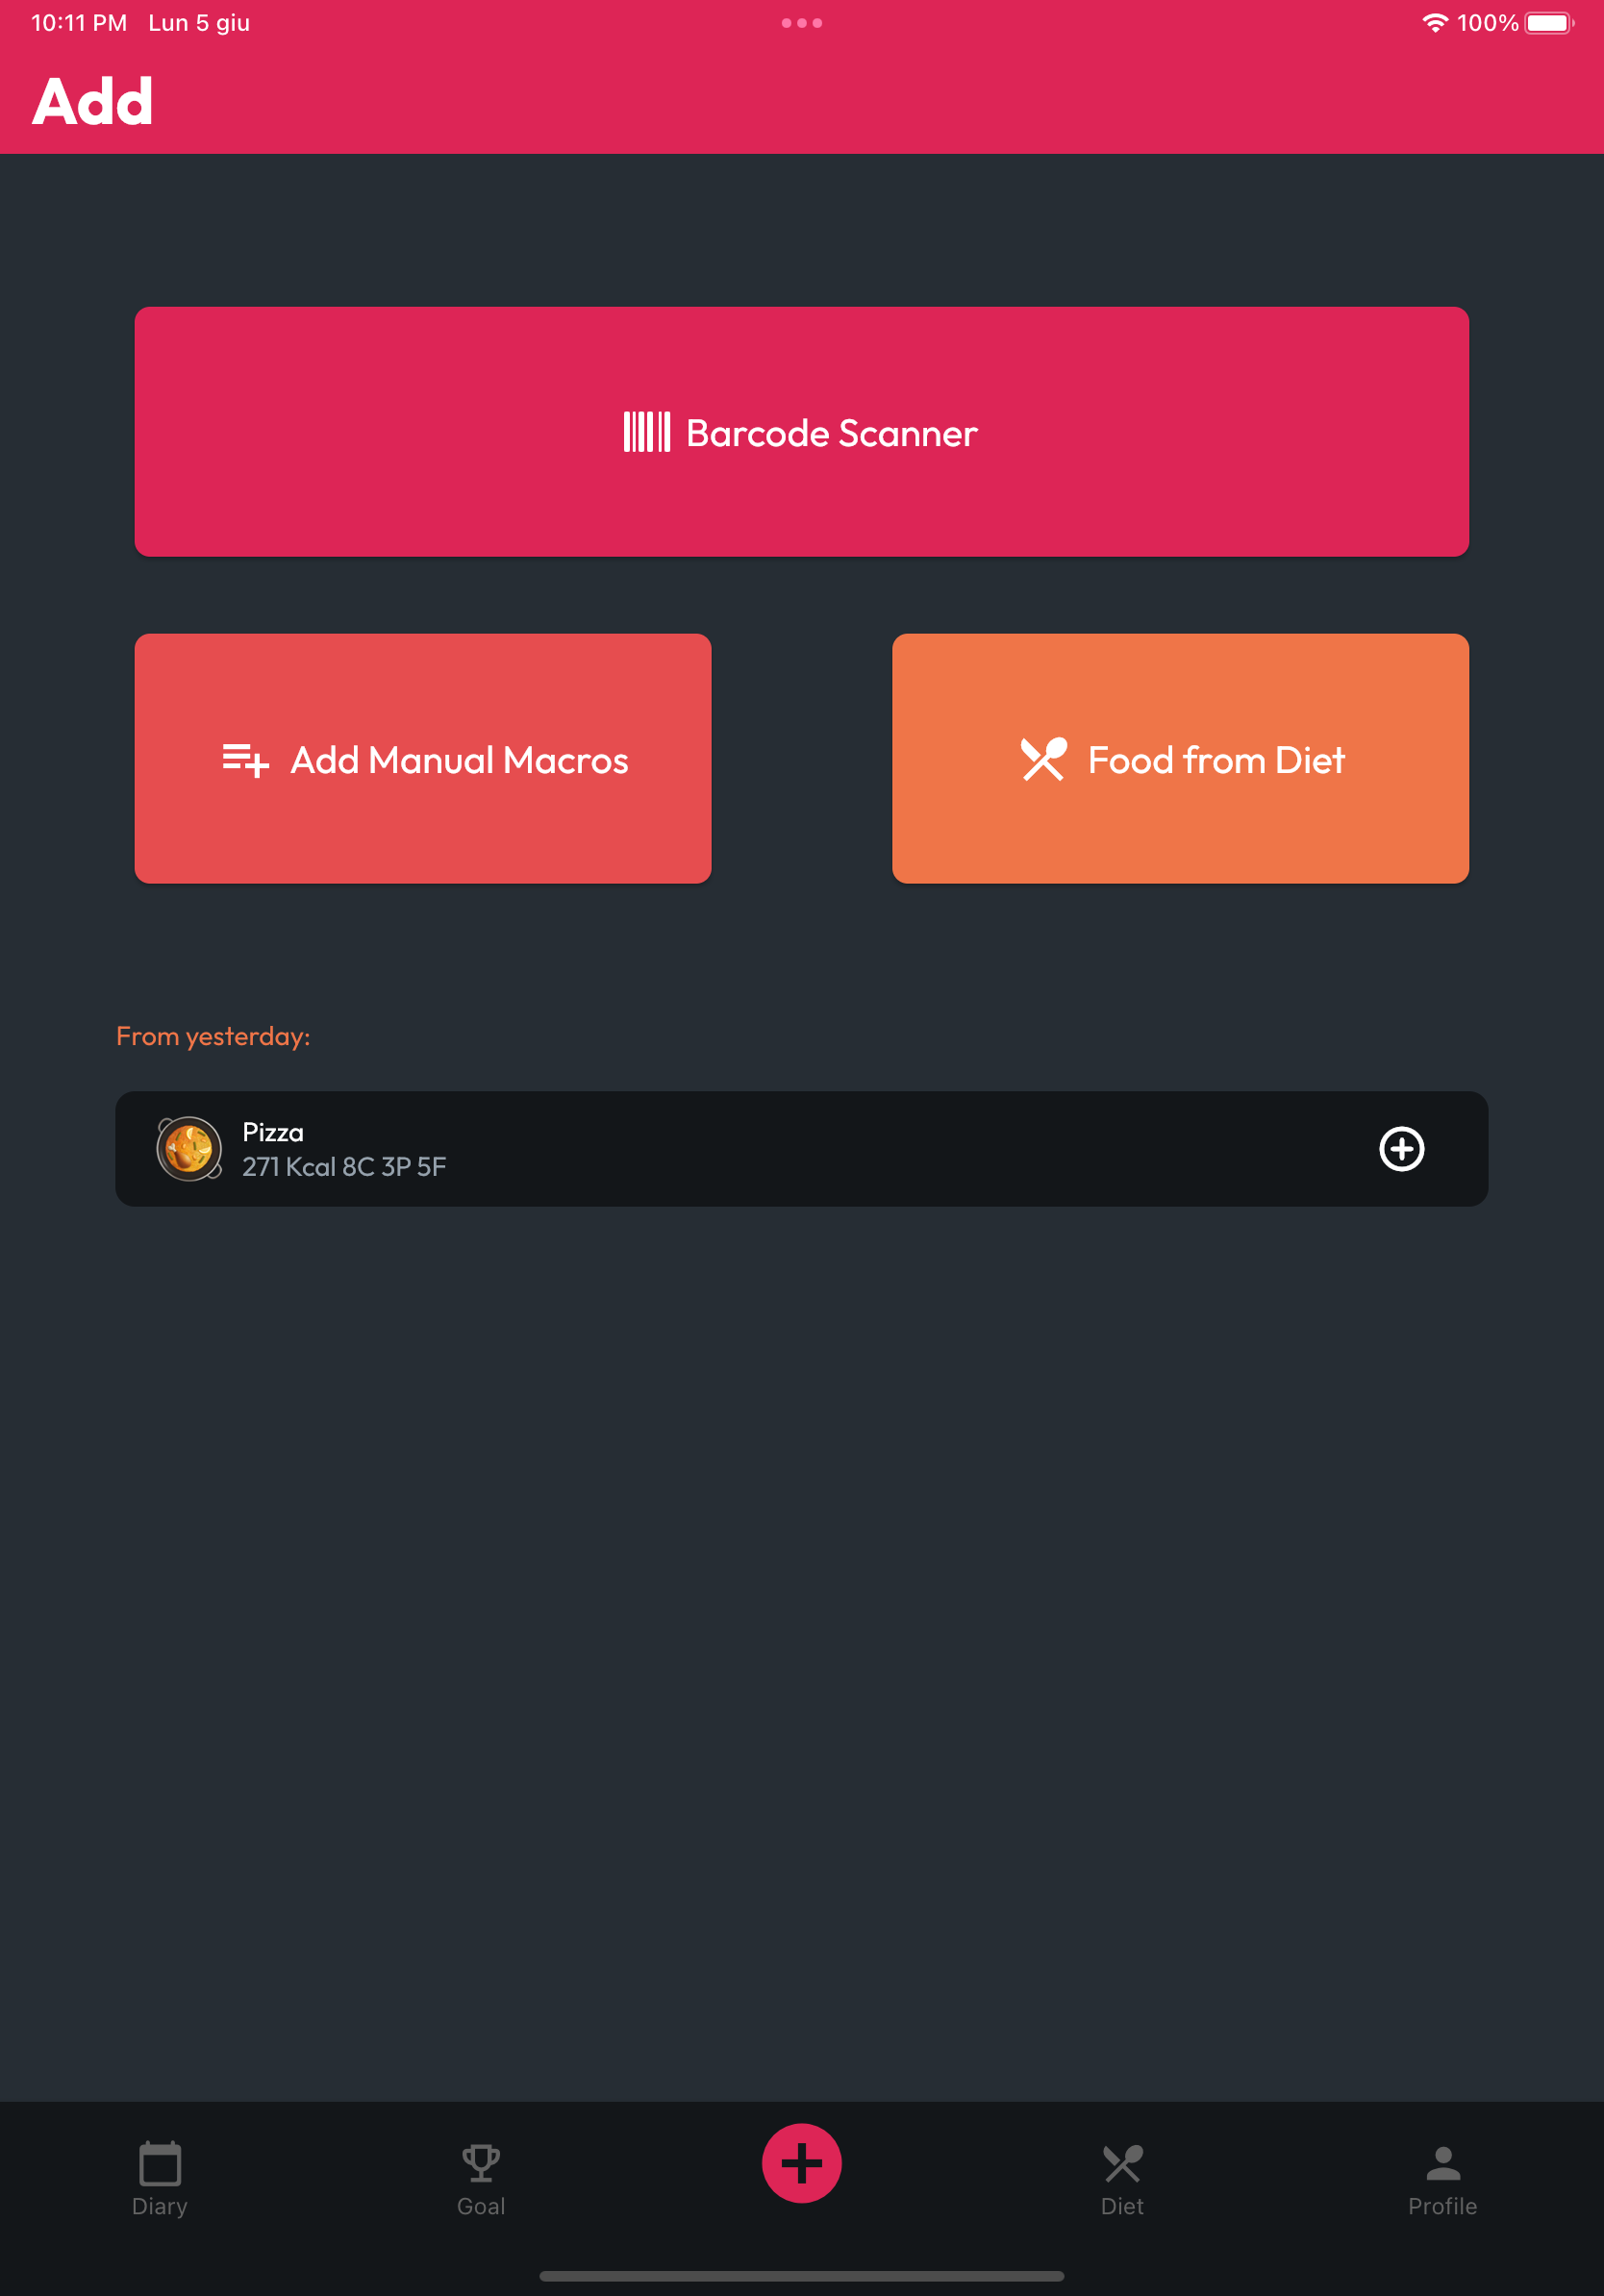
\includegraphics[scale=0.1]{Images/Screenshots/Tablet/AddTablet.png}
  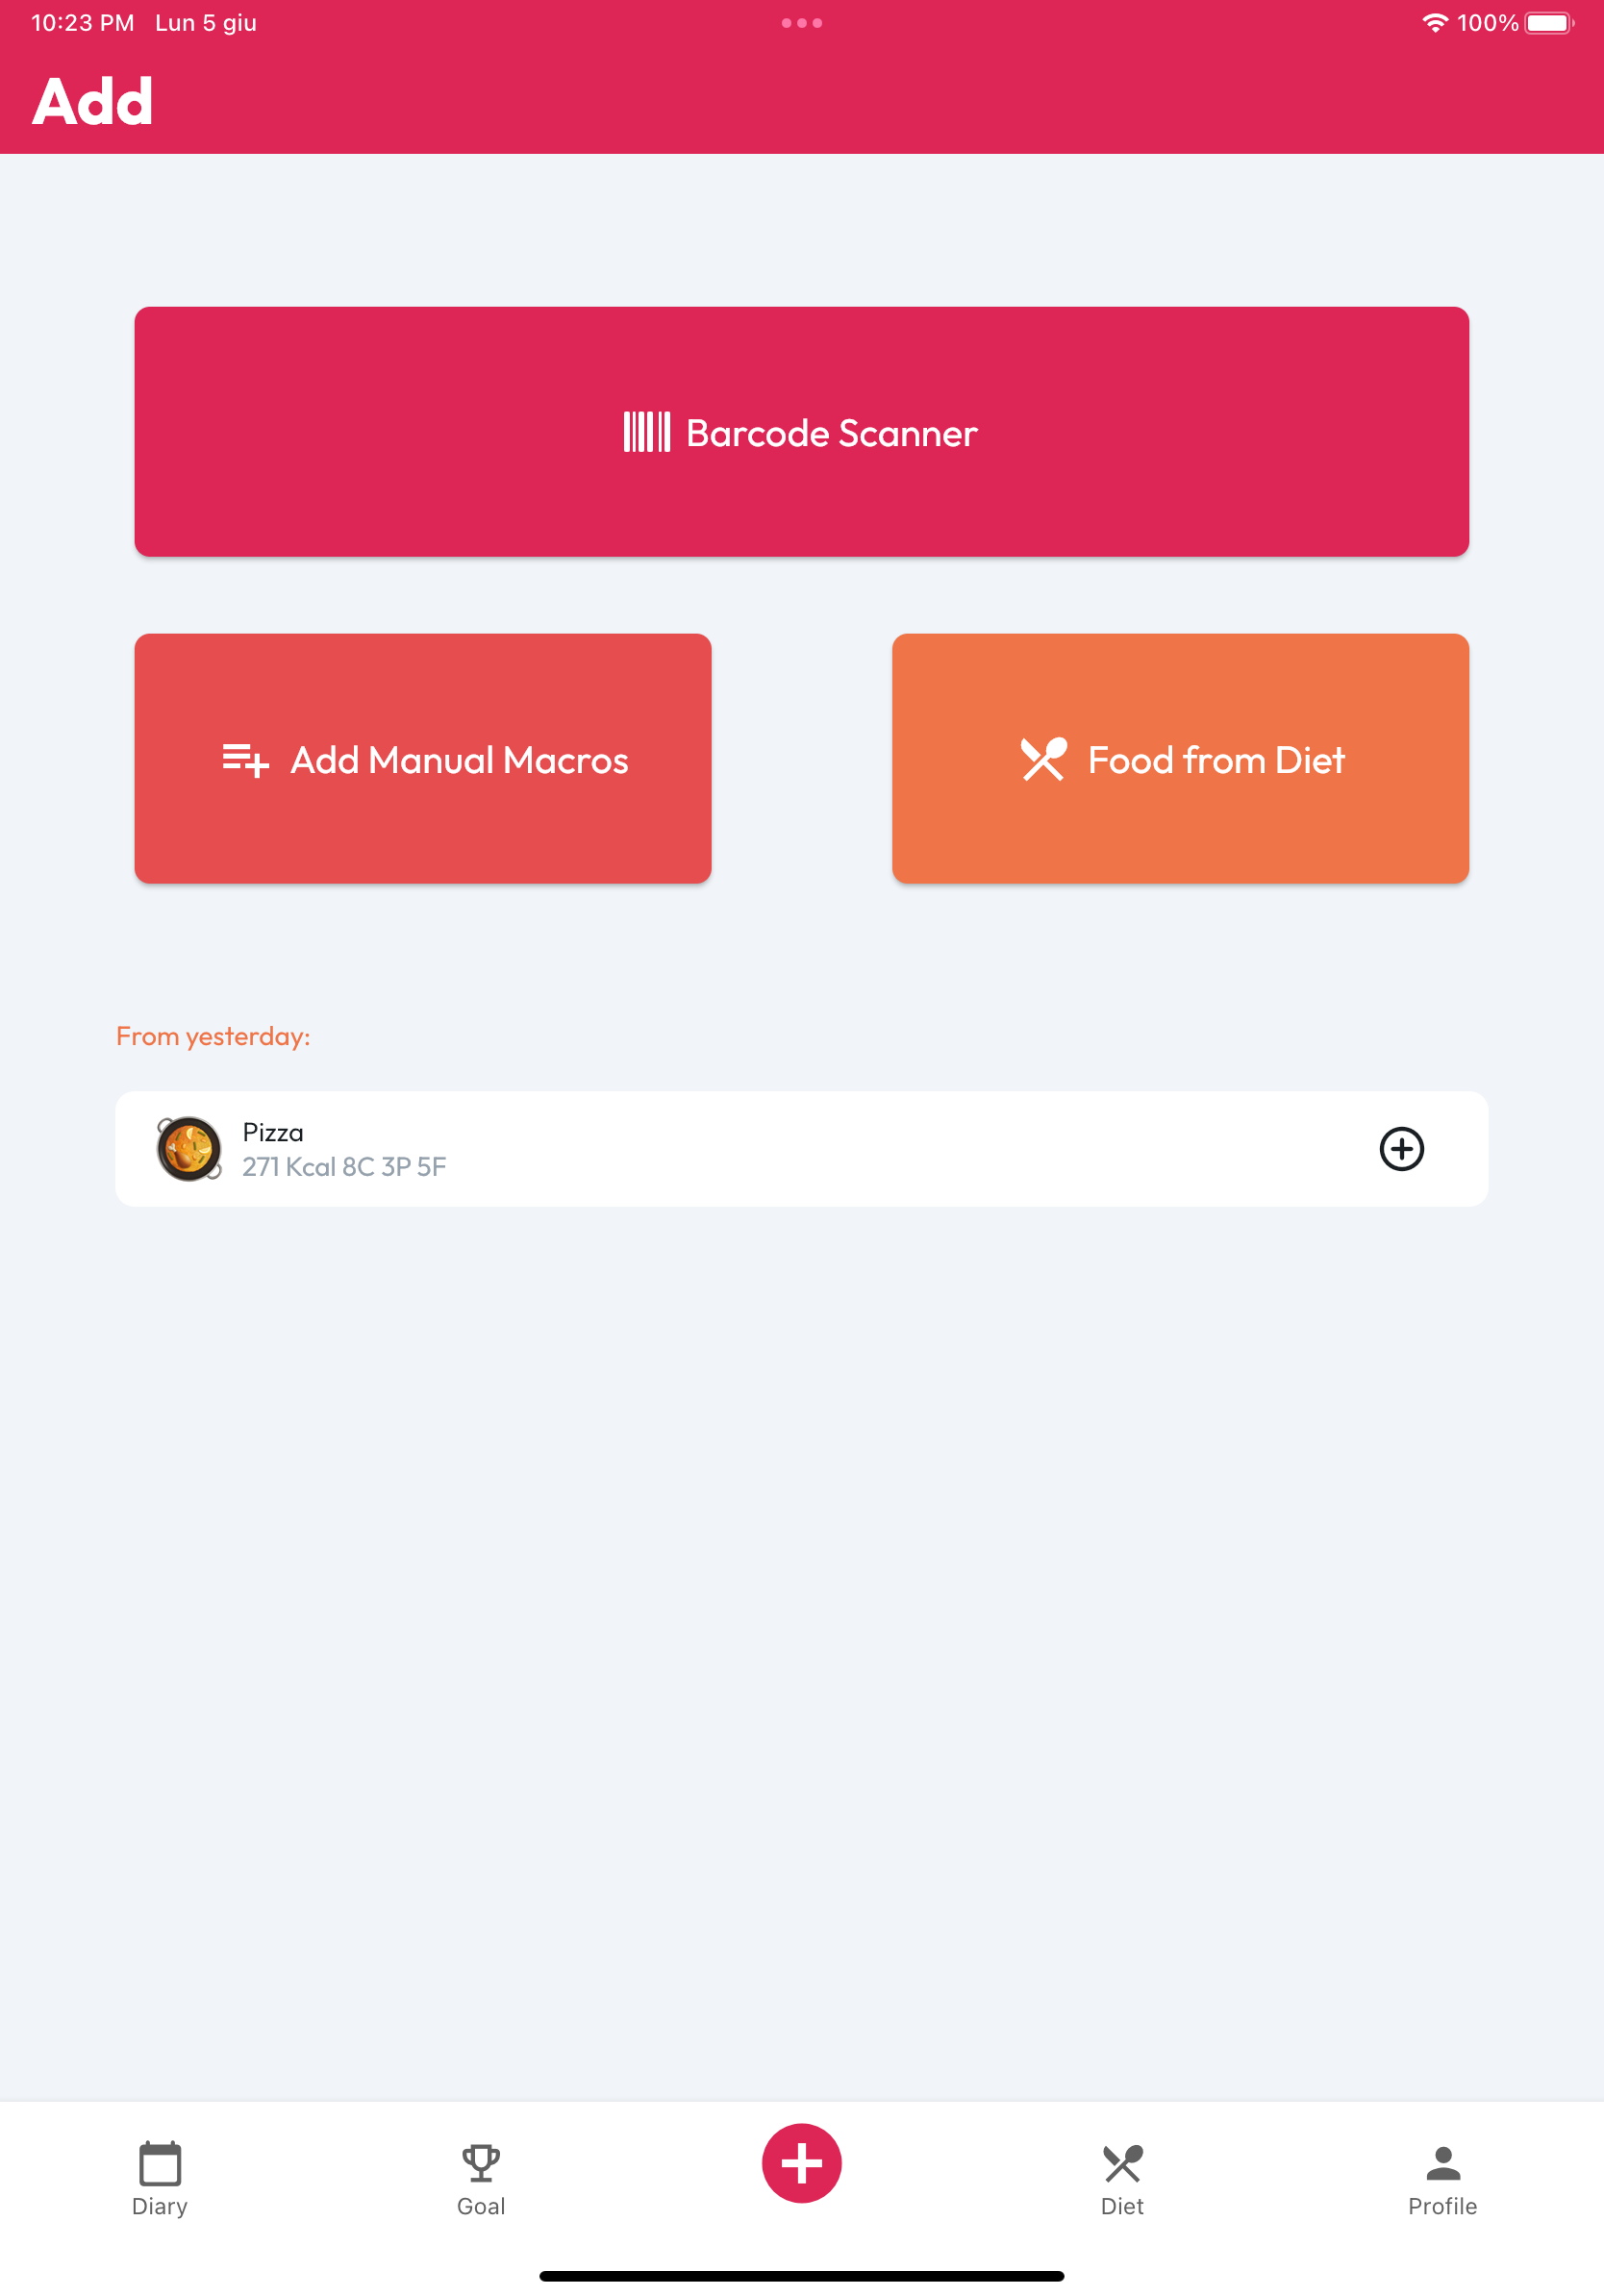
\includegraphics[scale=0.1]{Images/Screenshots/Tablet/AddTabletLight.png}
  \caption{Add tablet page}
\end{figure}

\clearpage

\subsection{Add food page}

\begin{figure}[!h]
  \centering
  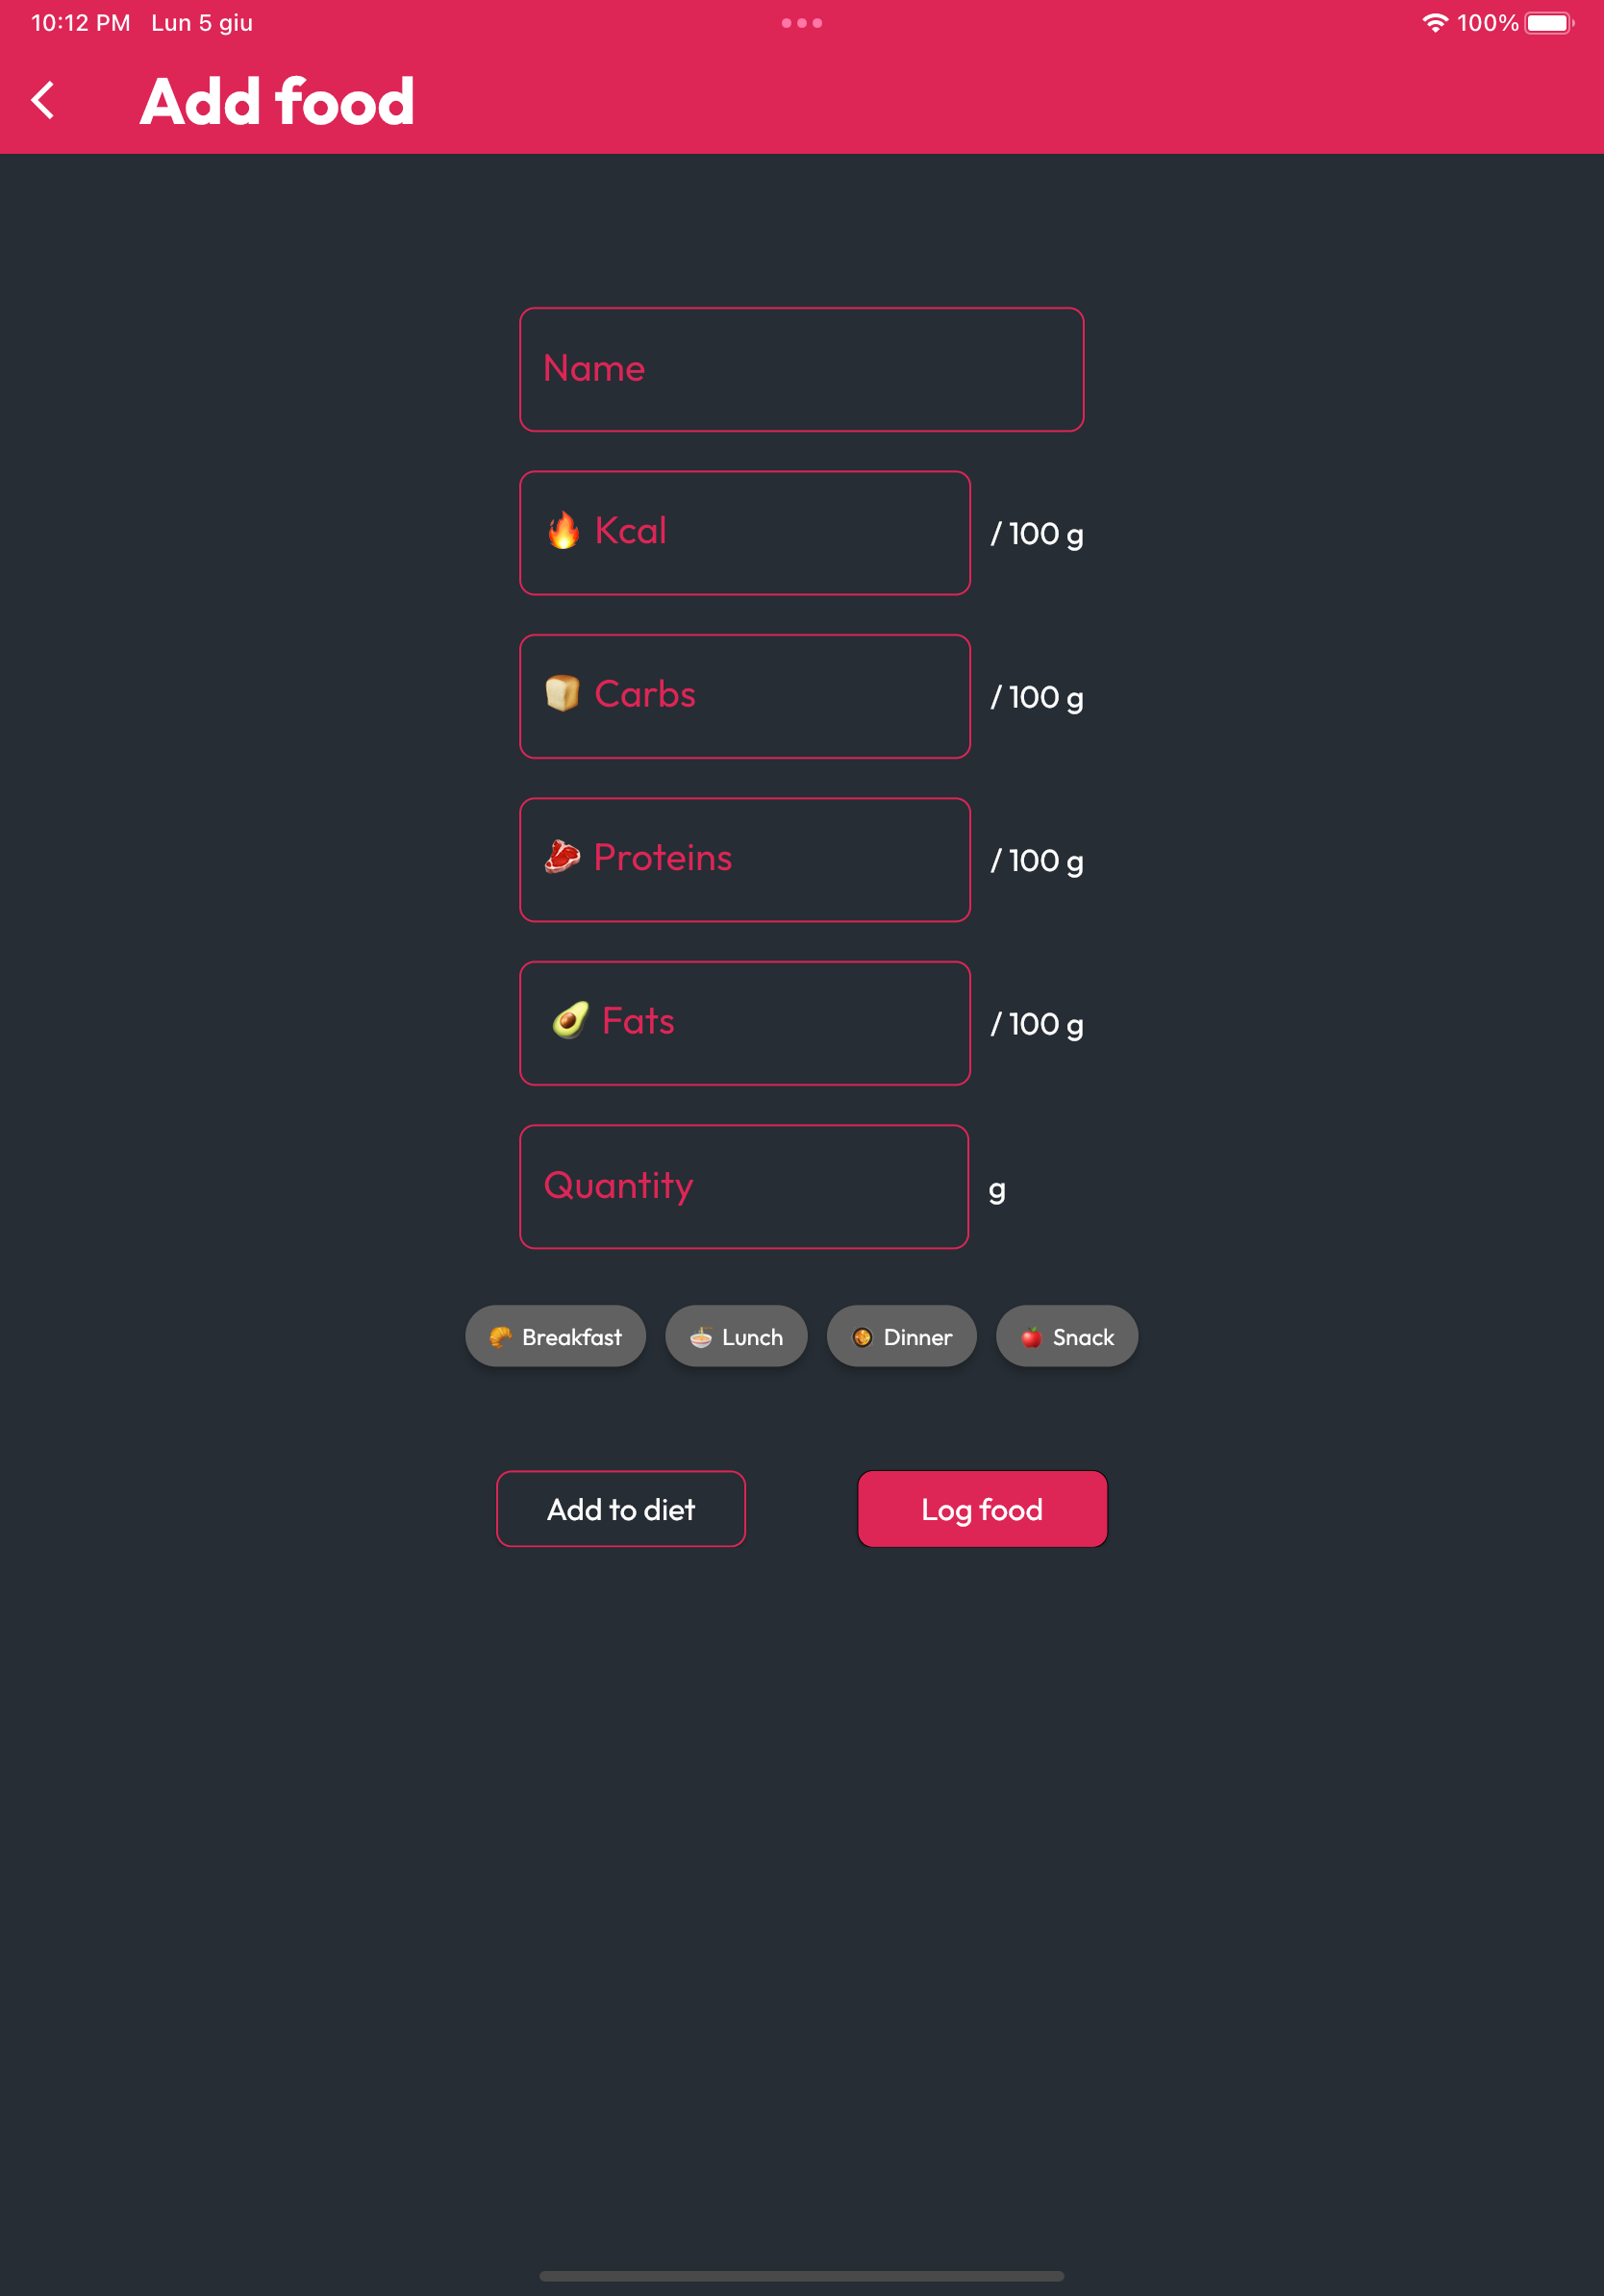
\includegraphics[scale=0.1]{Images/Screenshots/Tablet/AddFoodTablet.png}
  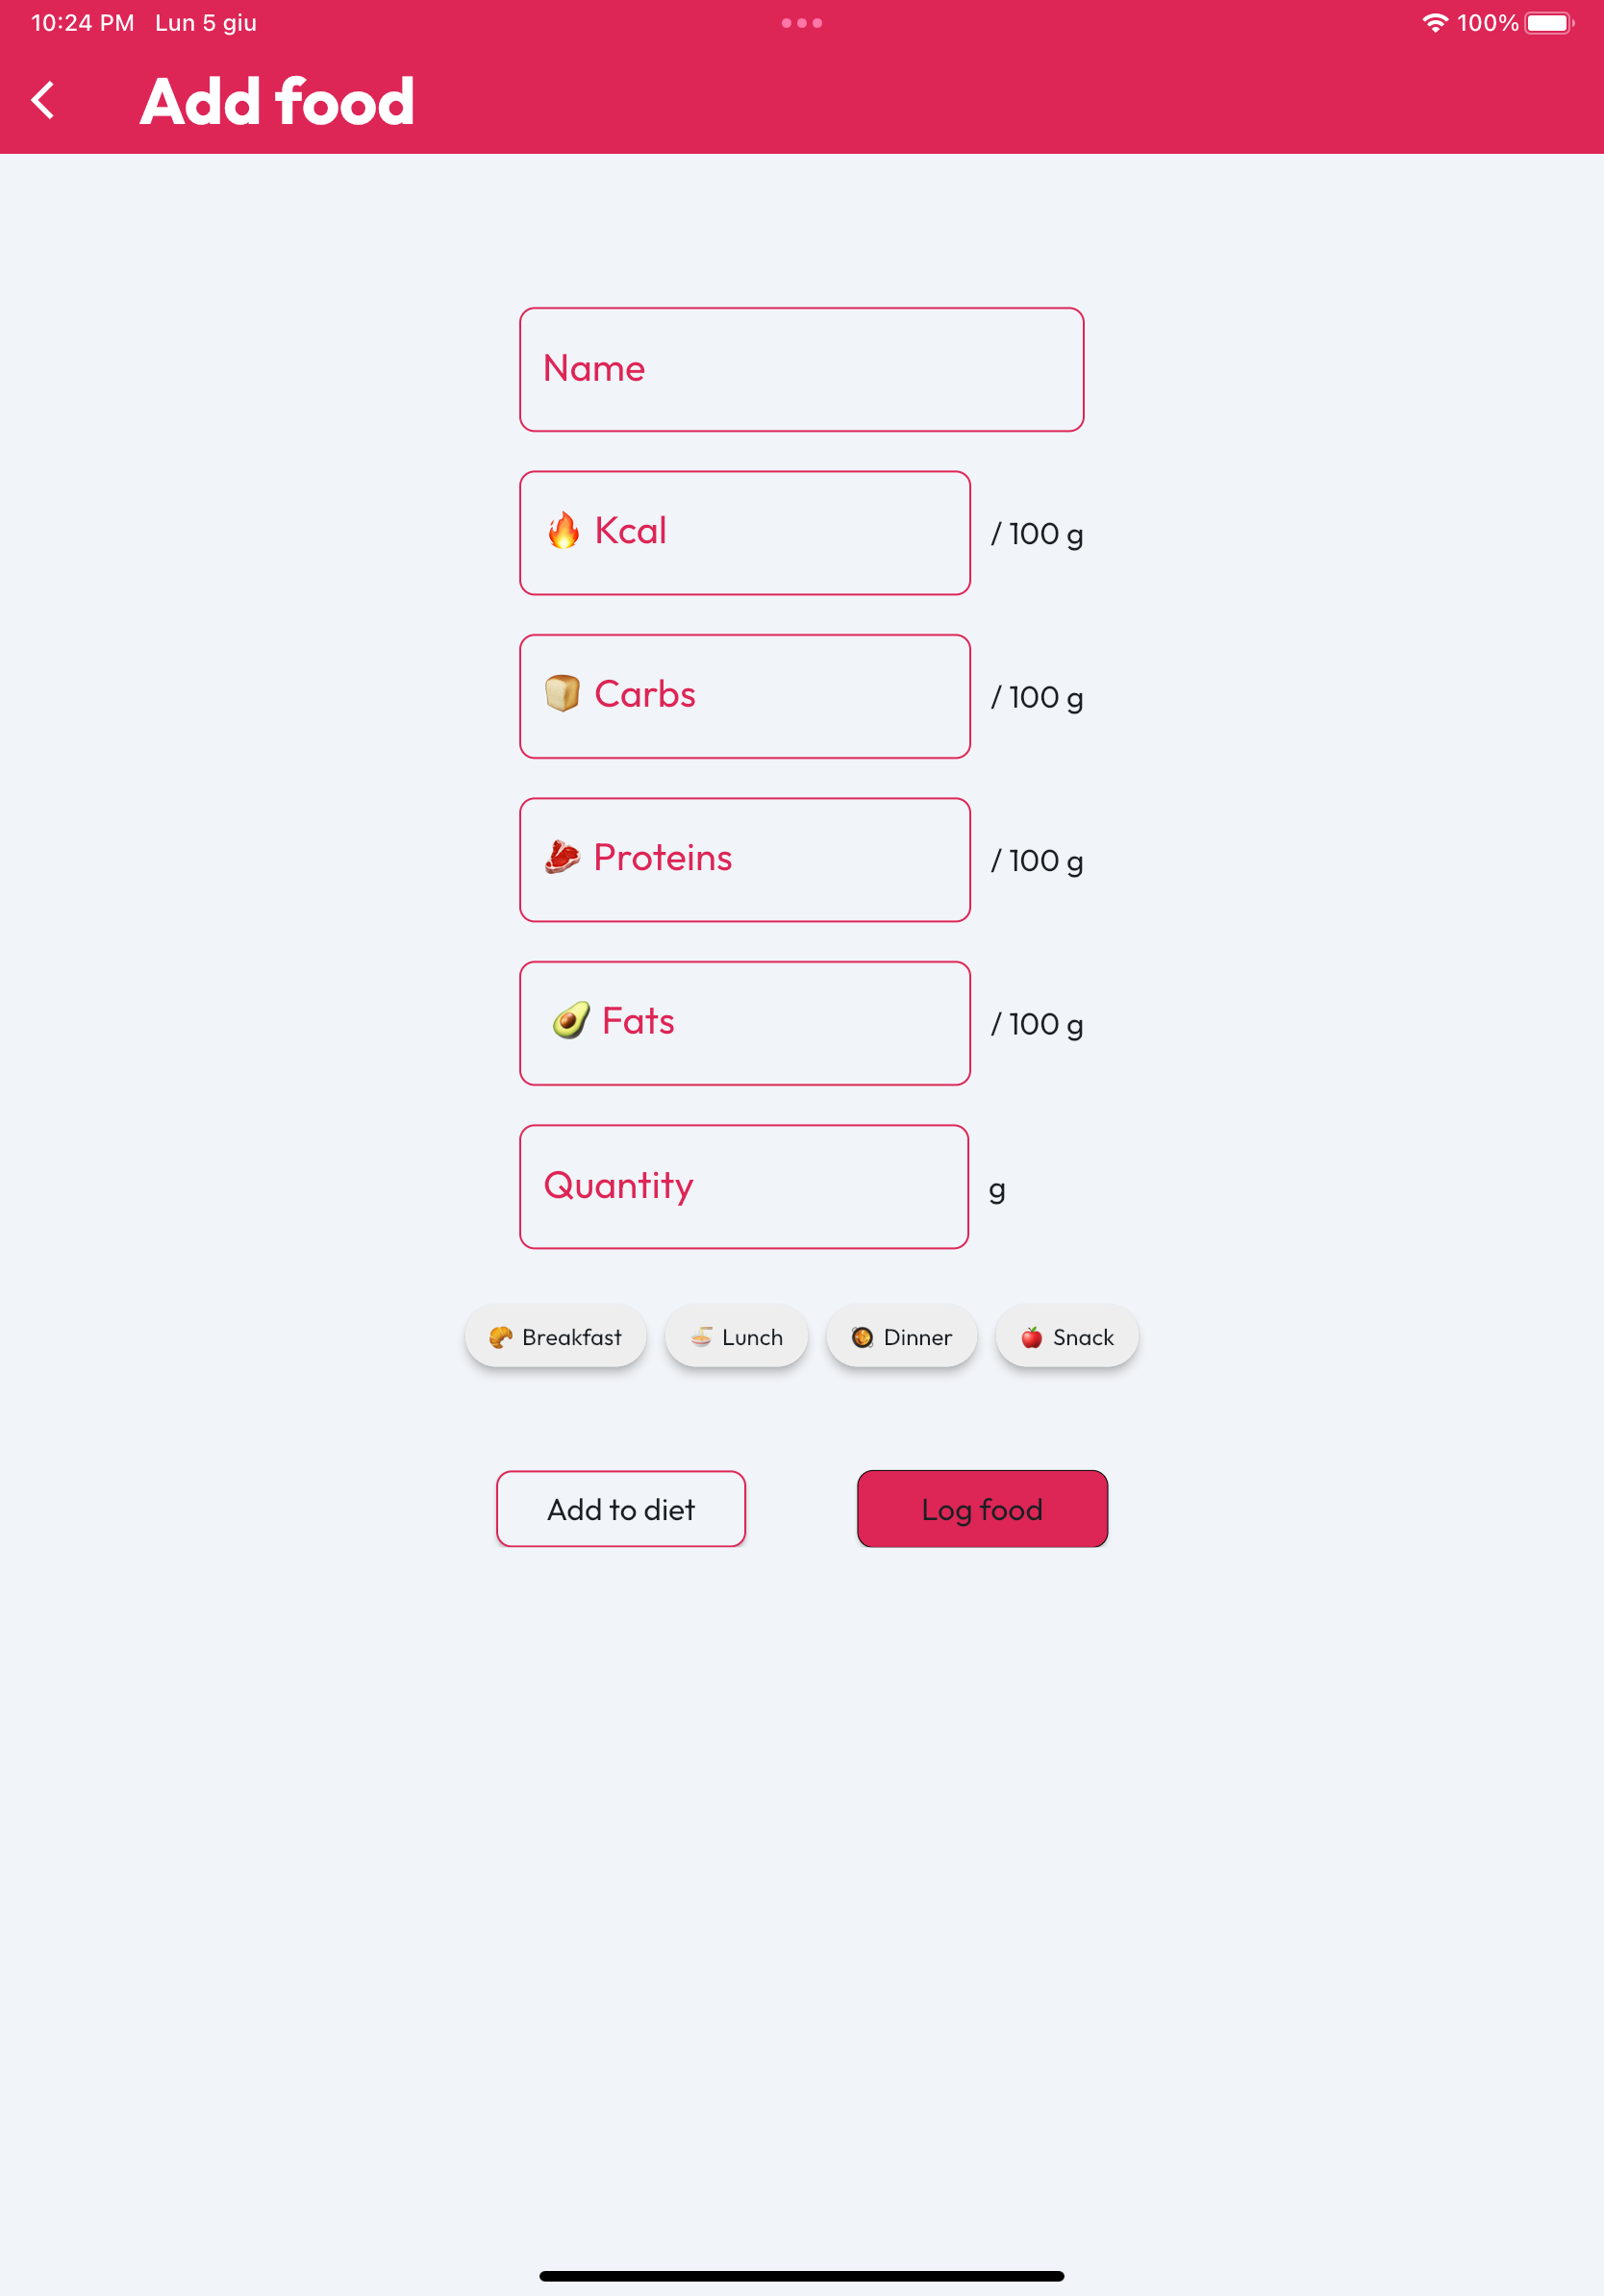
\includegraphics[scale=0.1]{Images/Screenshots/Tablet/AddFoodTabletLight.png}
  \caption{Add food tablet page}
\end{figure}

\clearpage

\subsection{Diet page}

\begin{figure}[!h]
  \centering
  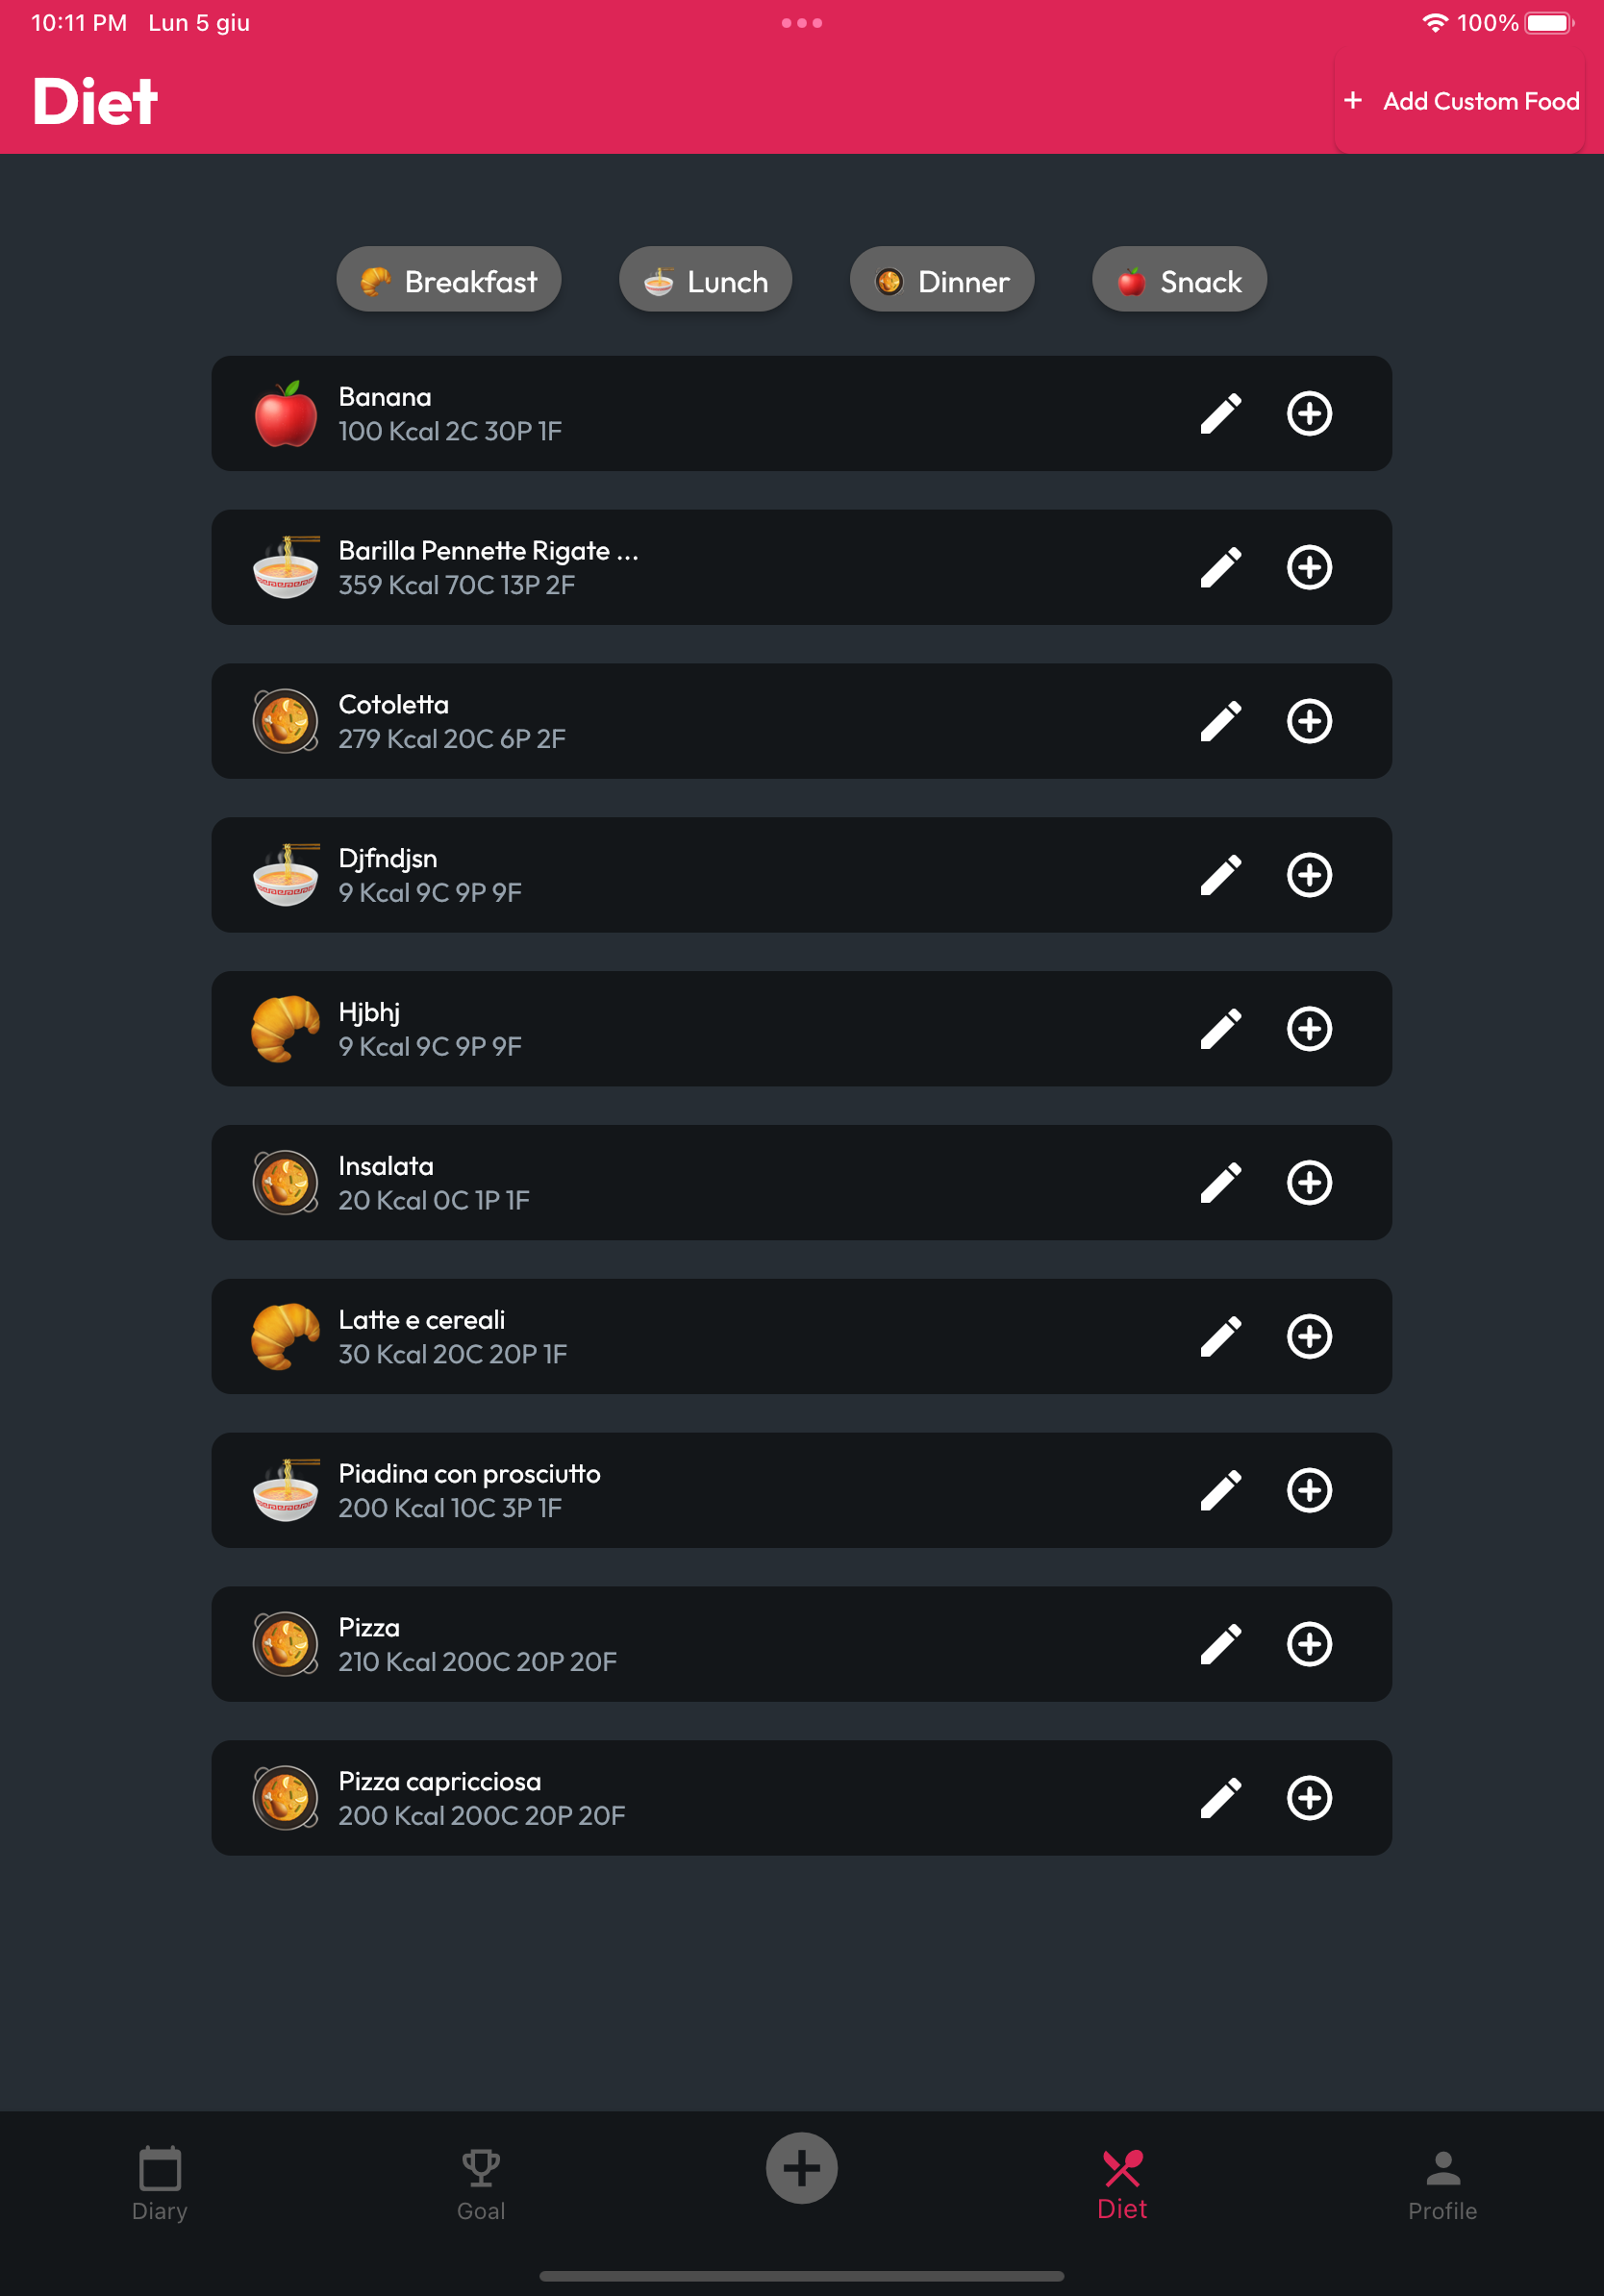
\includegraphics[scale=0.1]{Images/Screenshots/Tablet/DietTablet.png}
  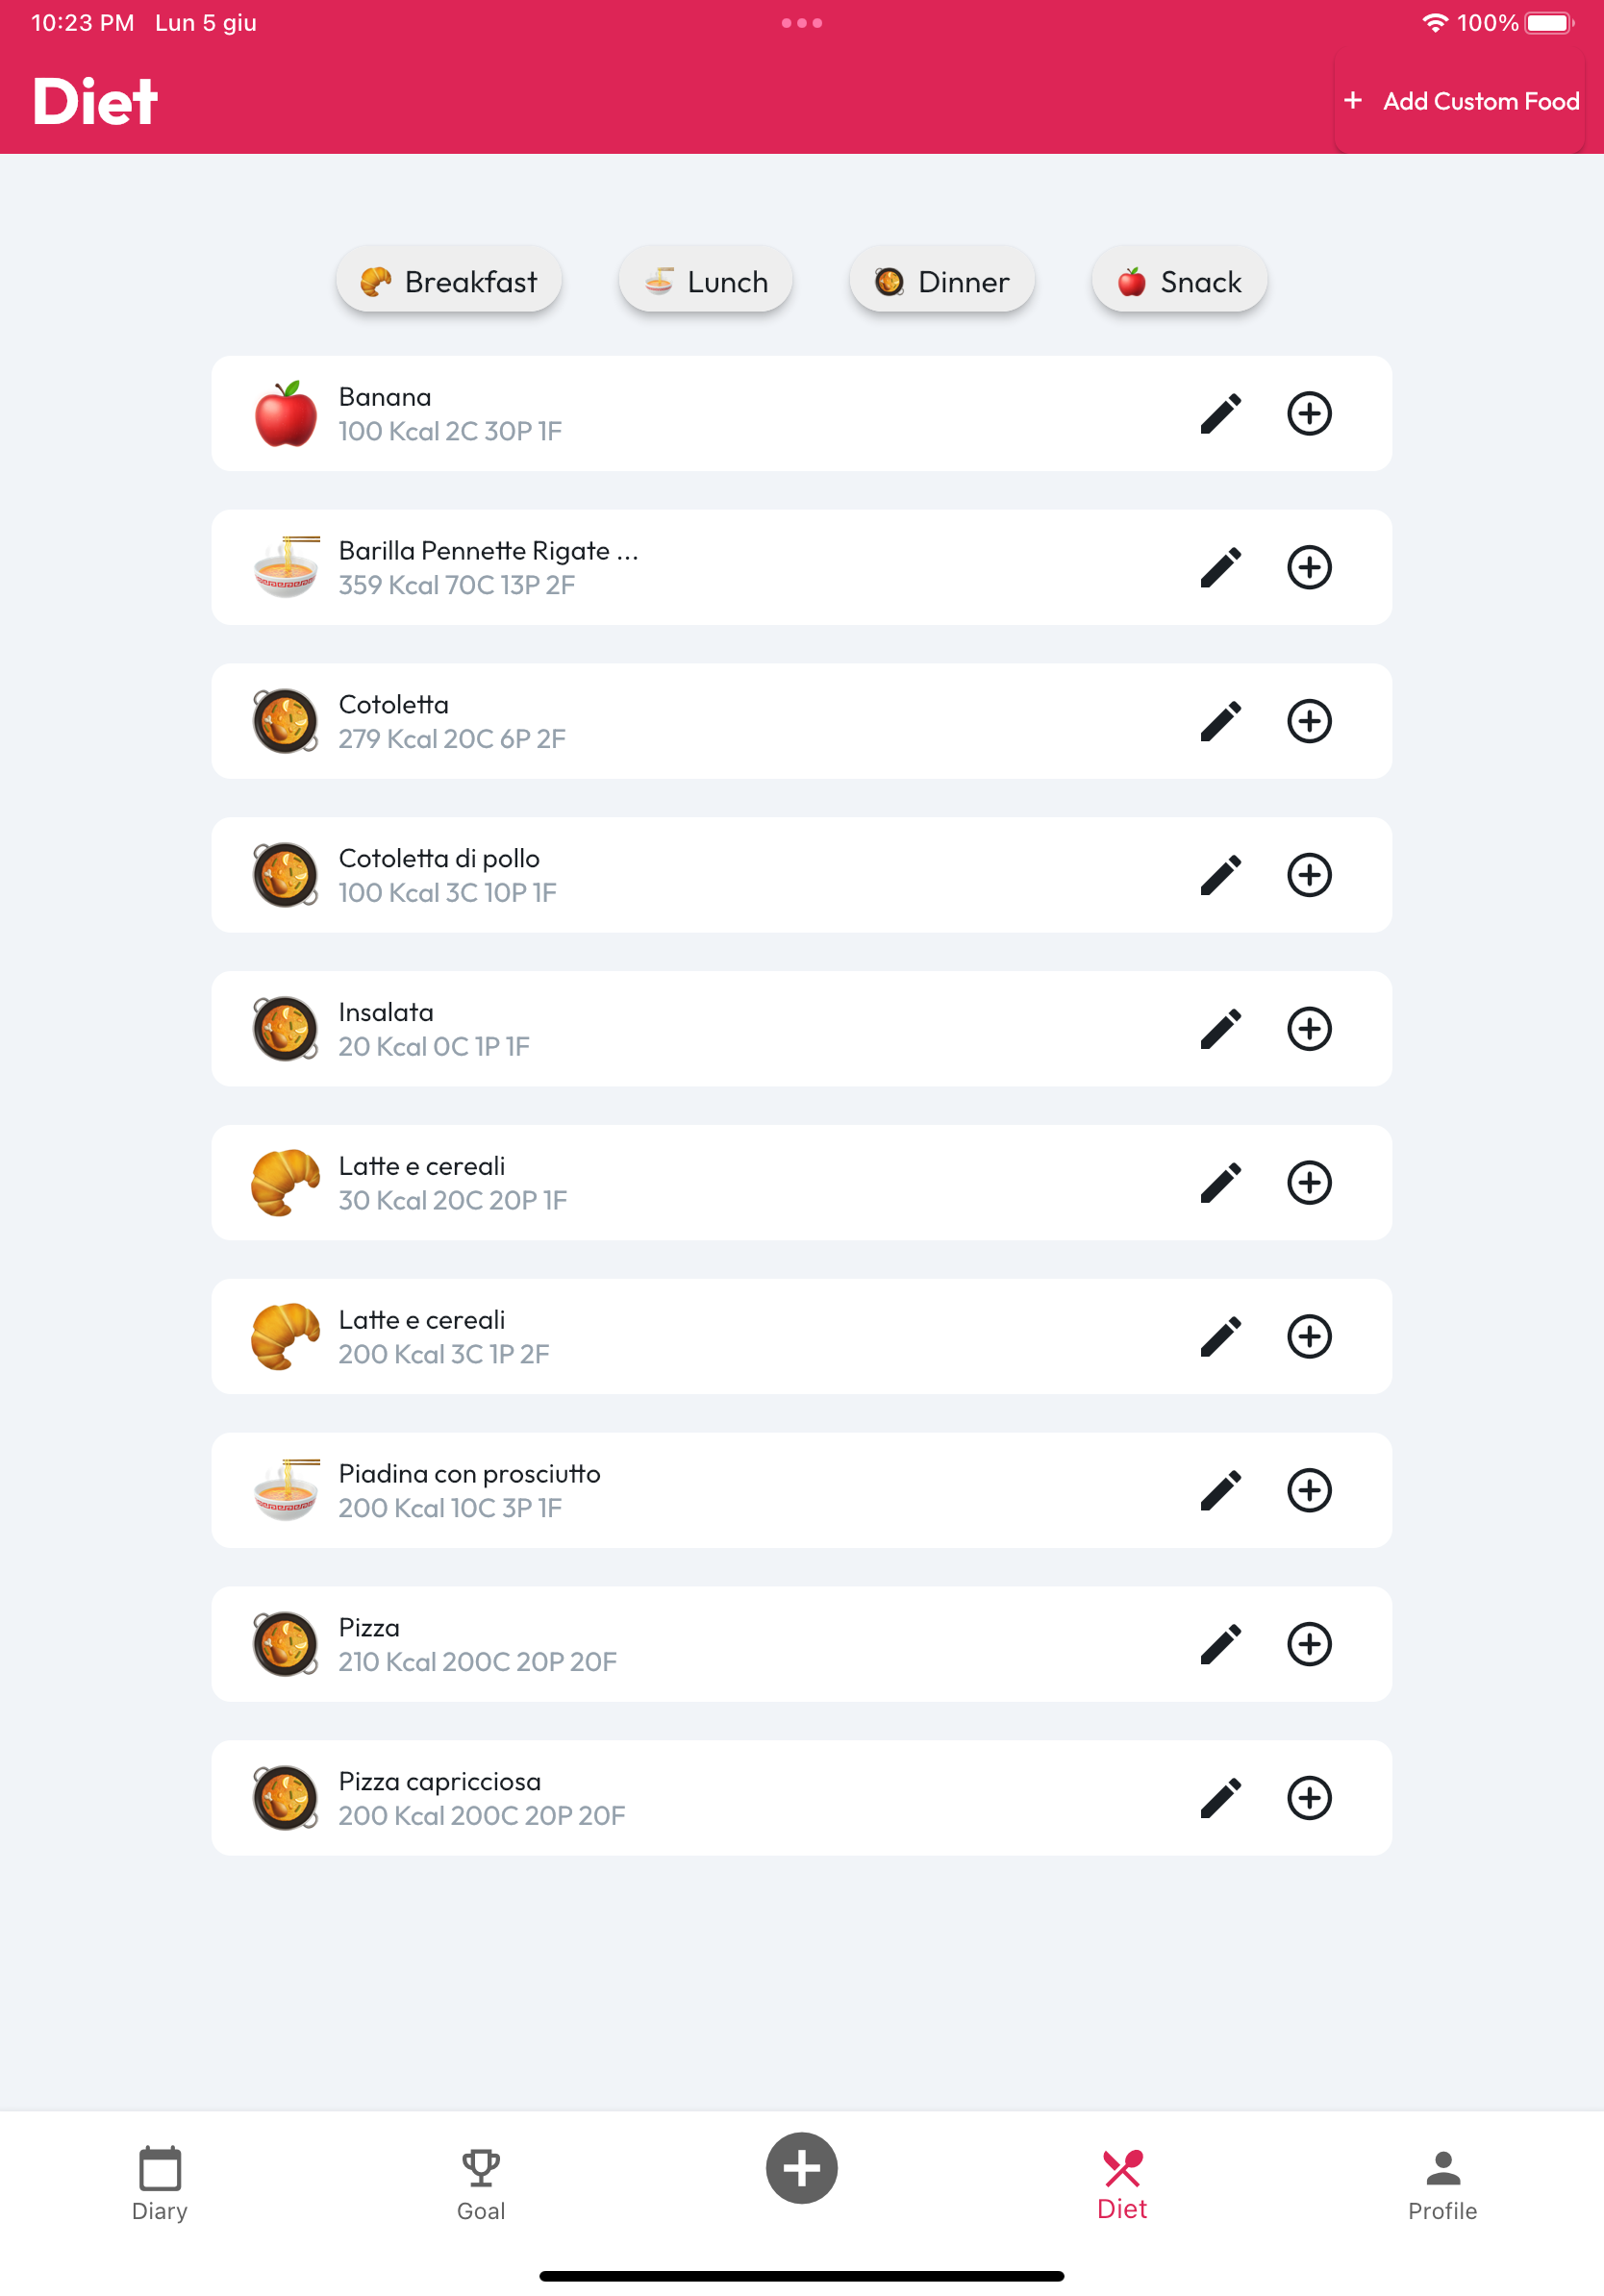
\includegraphics[scale=0.1]{Images/Screenshots/Tablet/DietTabletLight.png}
  \caption{Diet tablet page}
\end{figure}

\clearpage

\subsection{Profile page}

\begin{figure}[!h]
  \centering
  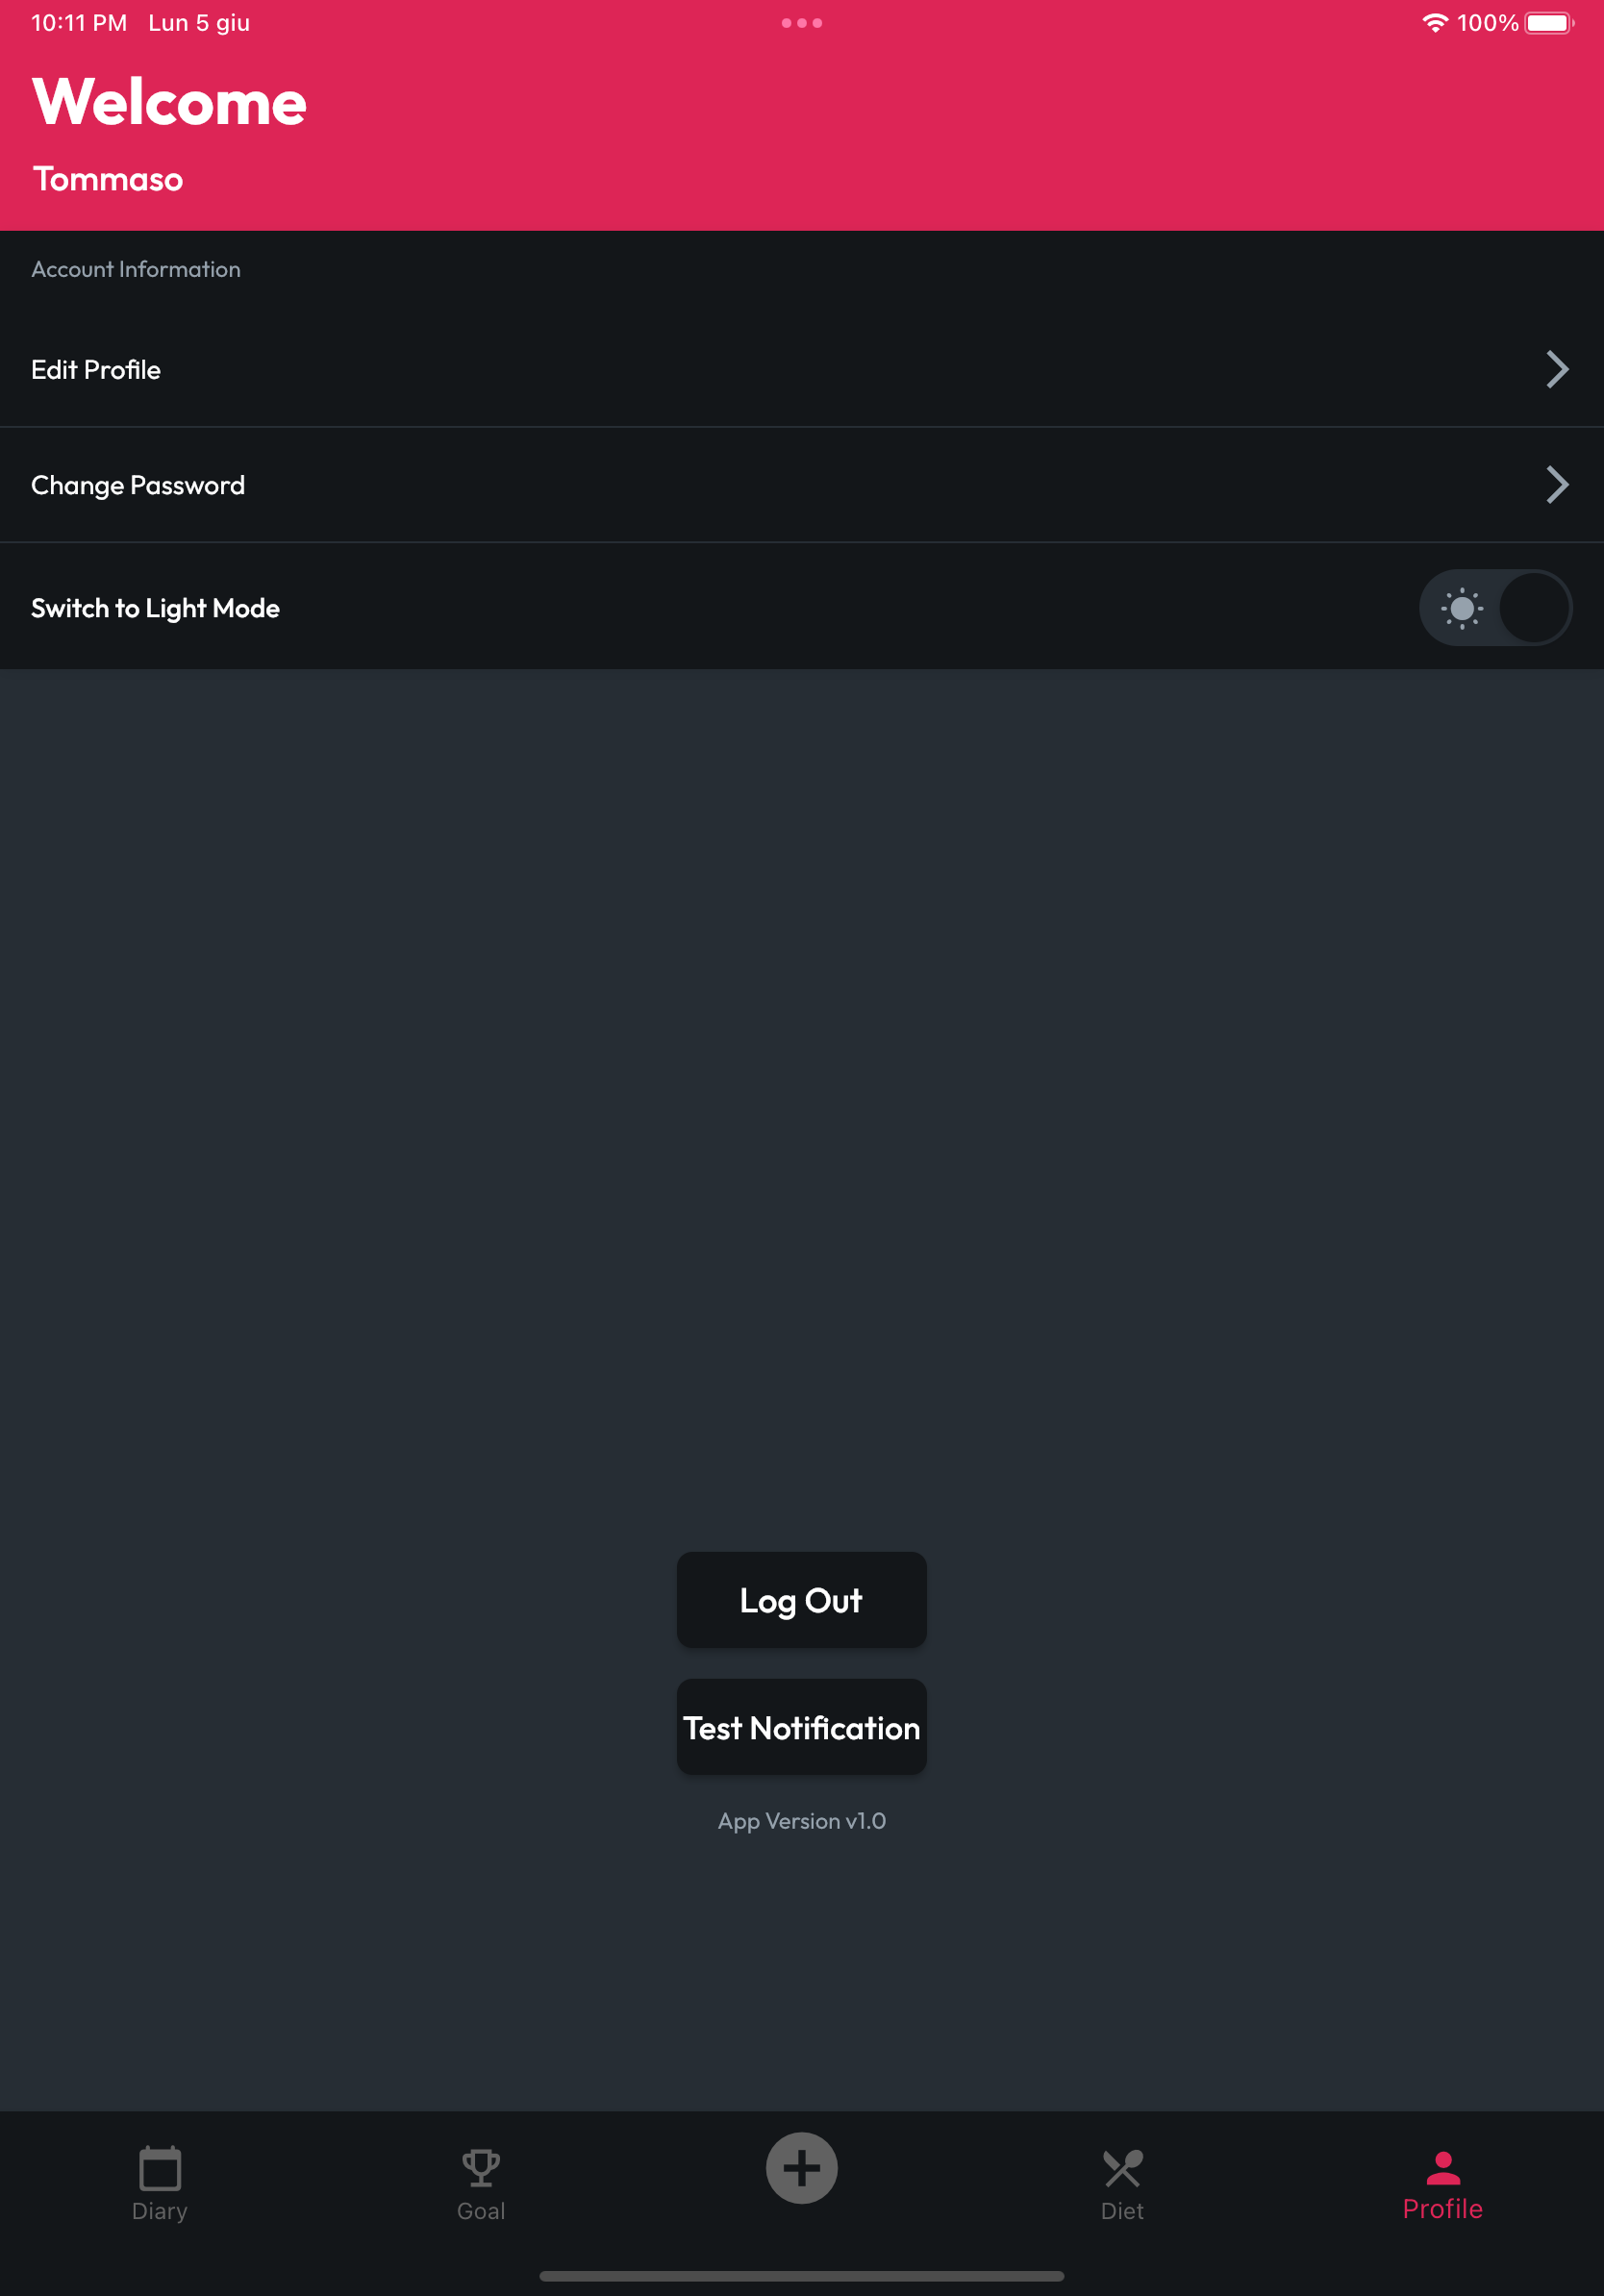
\includegraphics[scale=0.1]{Images/Screenshots/Tablet/ProfileTablet.png}
  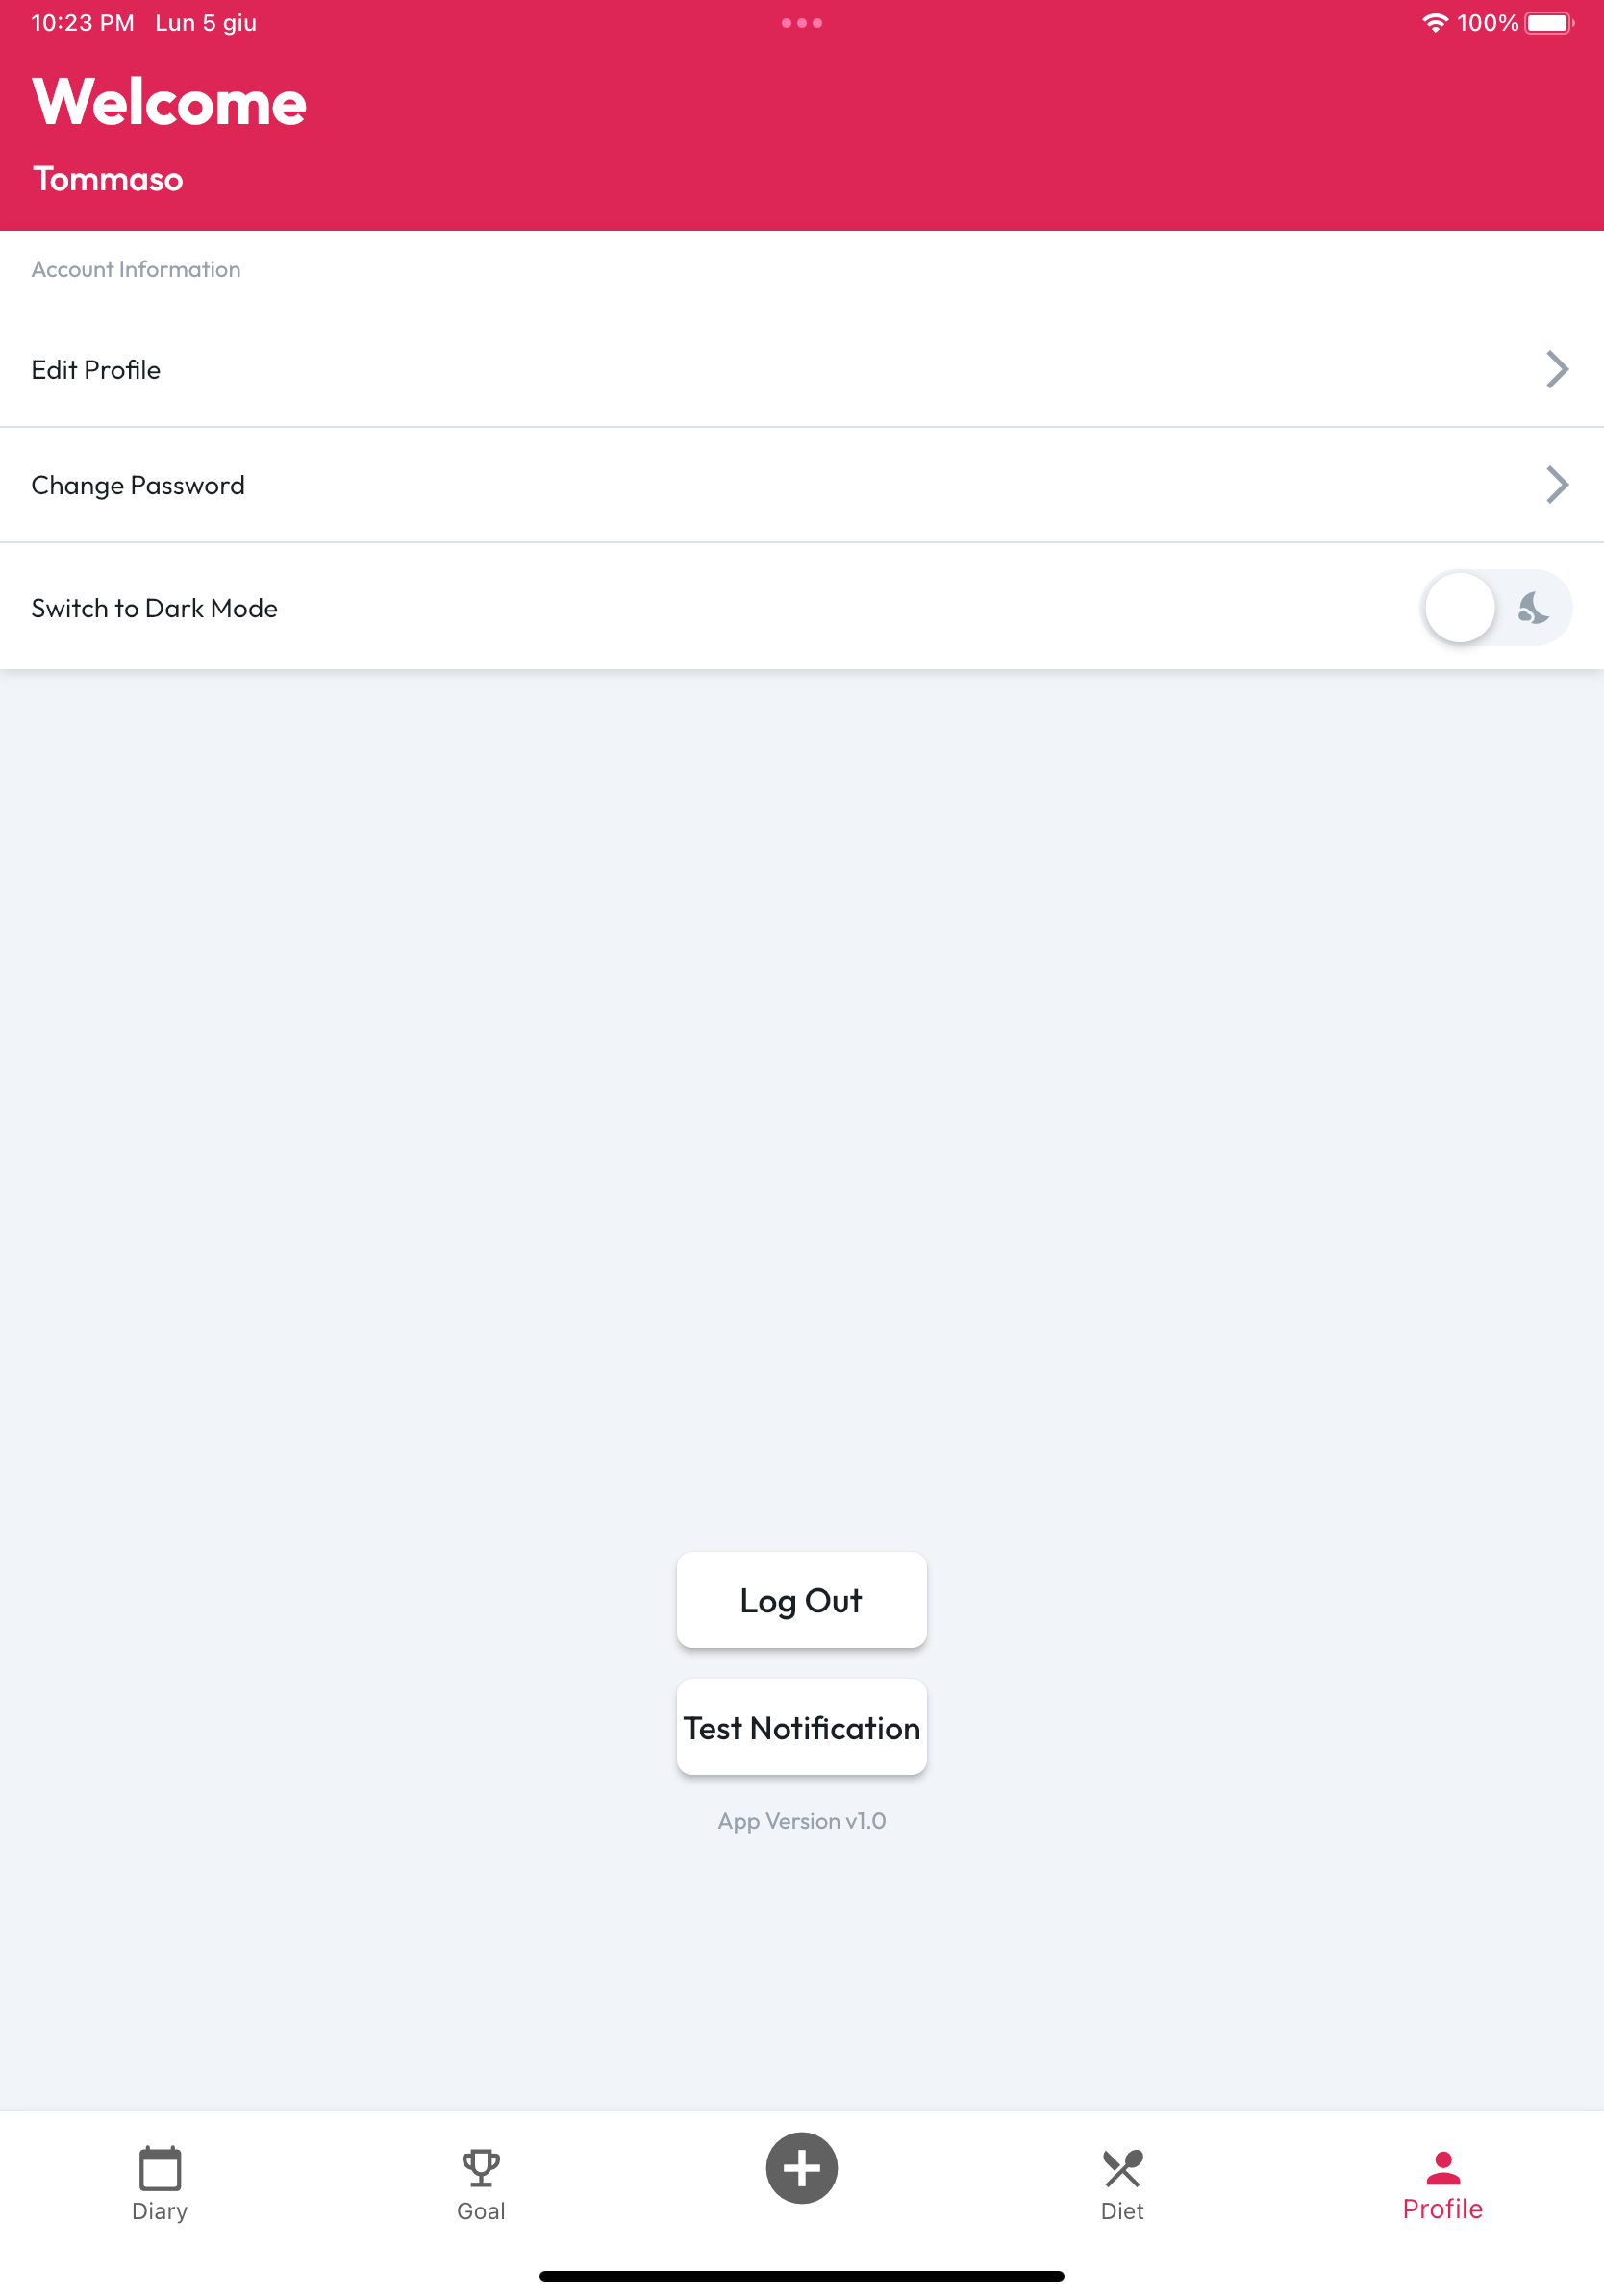
\includegraphics[scale=0.1]{Images/Screenshots/Tablet/ProfileTabletLight.png}
  \caption{Profile tablet page}
\end{figure}

\clearpage

\section{UX Flow}

\begin{minipage}{\linewidth}
    This diagram shows the actions that the user can perform to navigate through the screens of the app. \\
    (For convenience it has been used mobile screens with dark mode.)
\end{minipage}

\begin{figure}[!h]
  \centering
  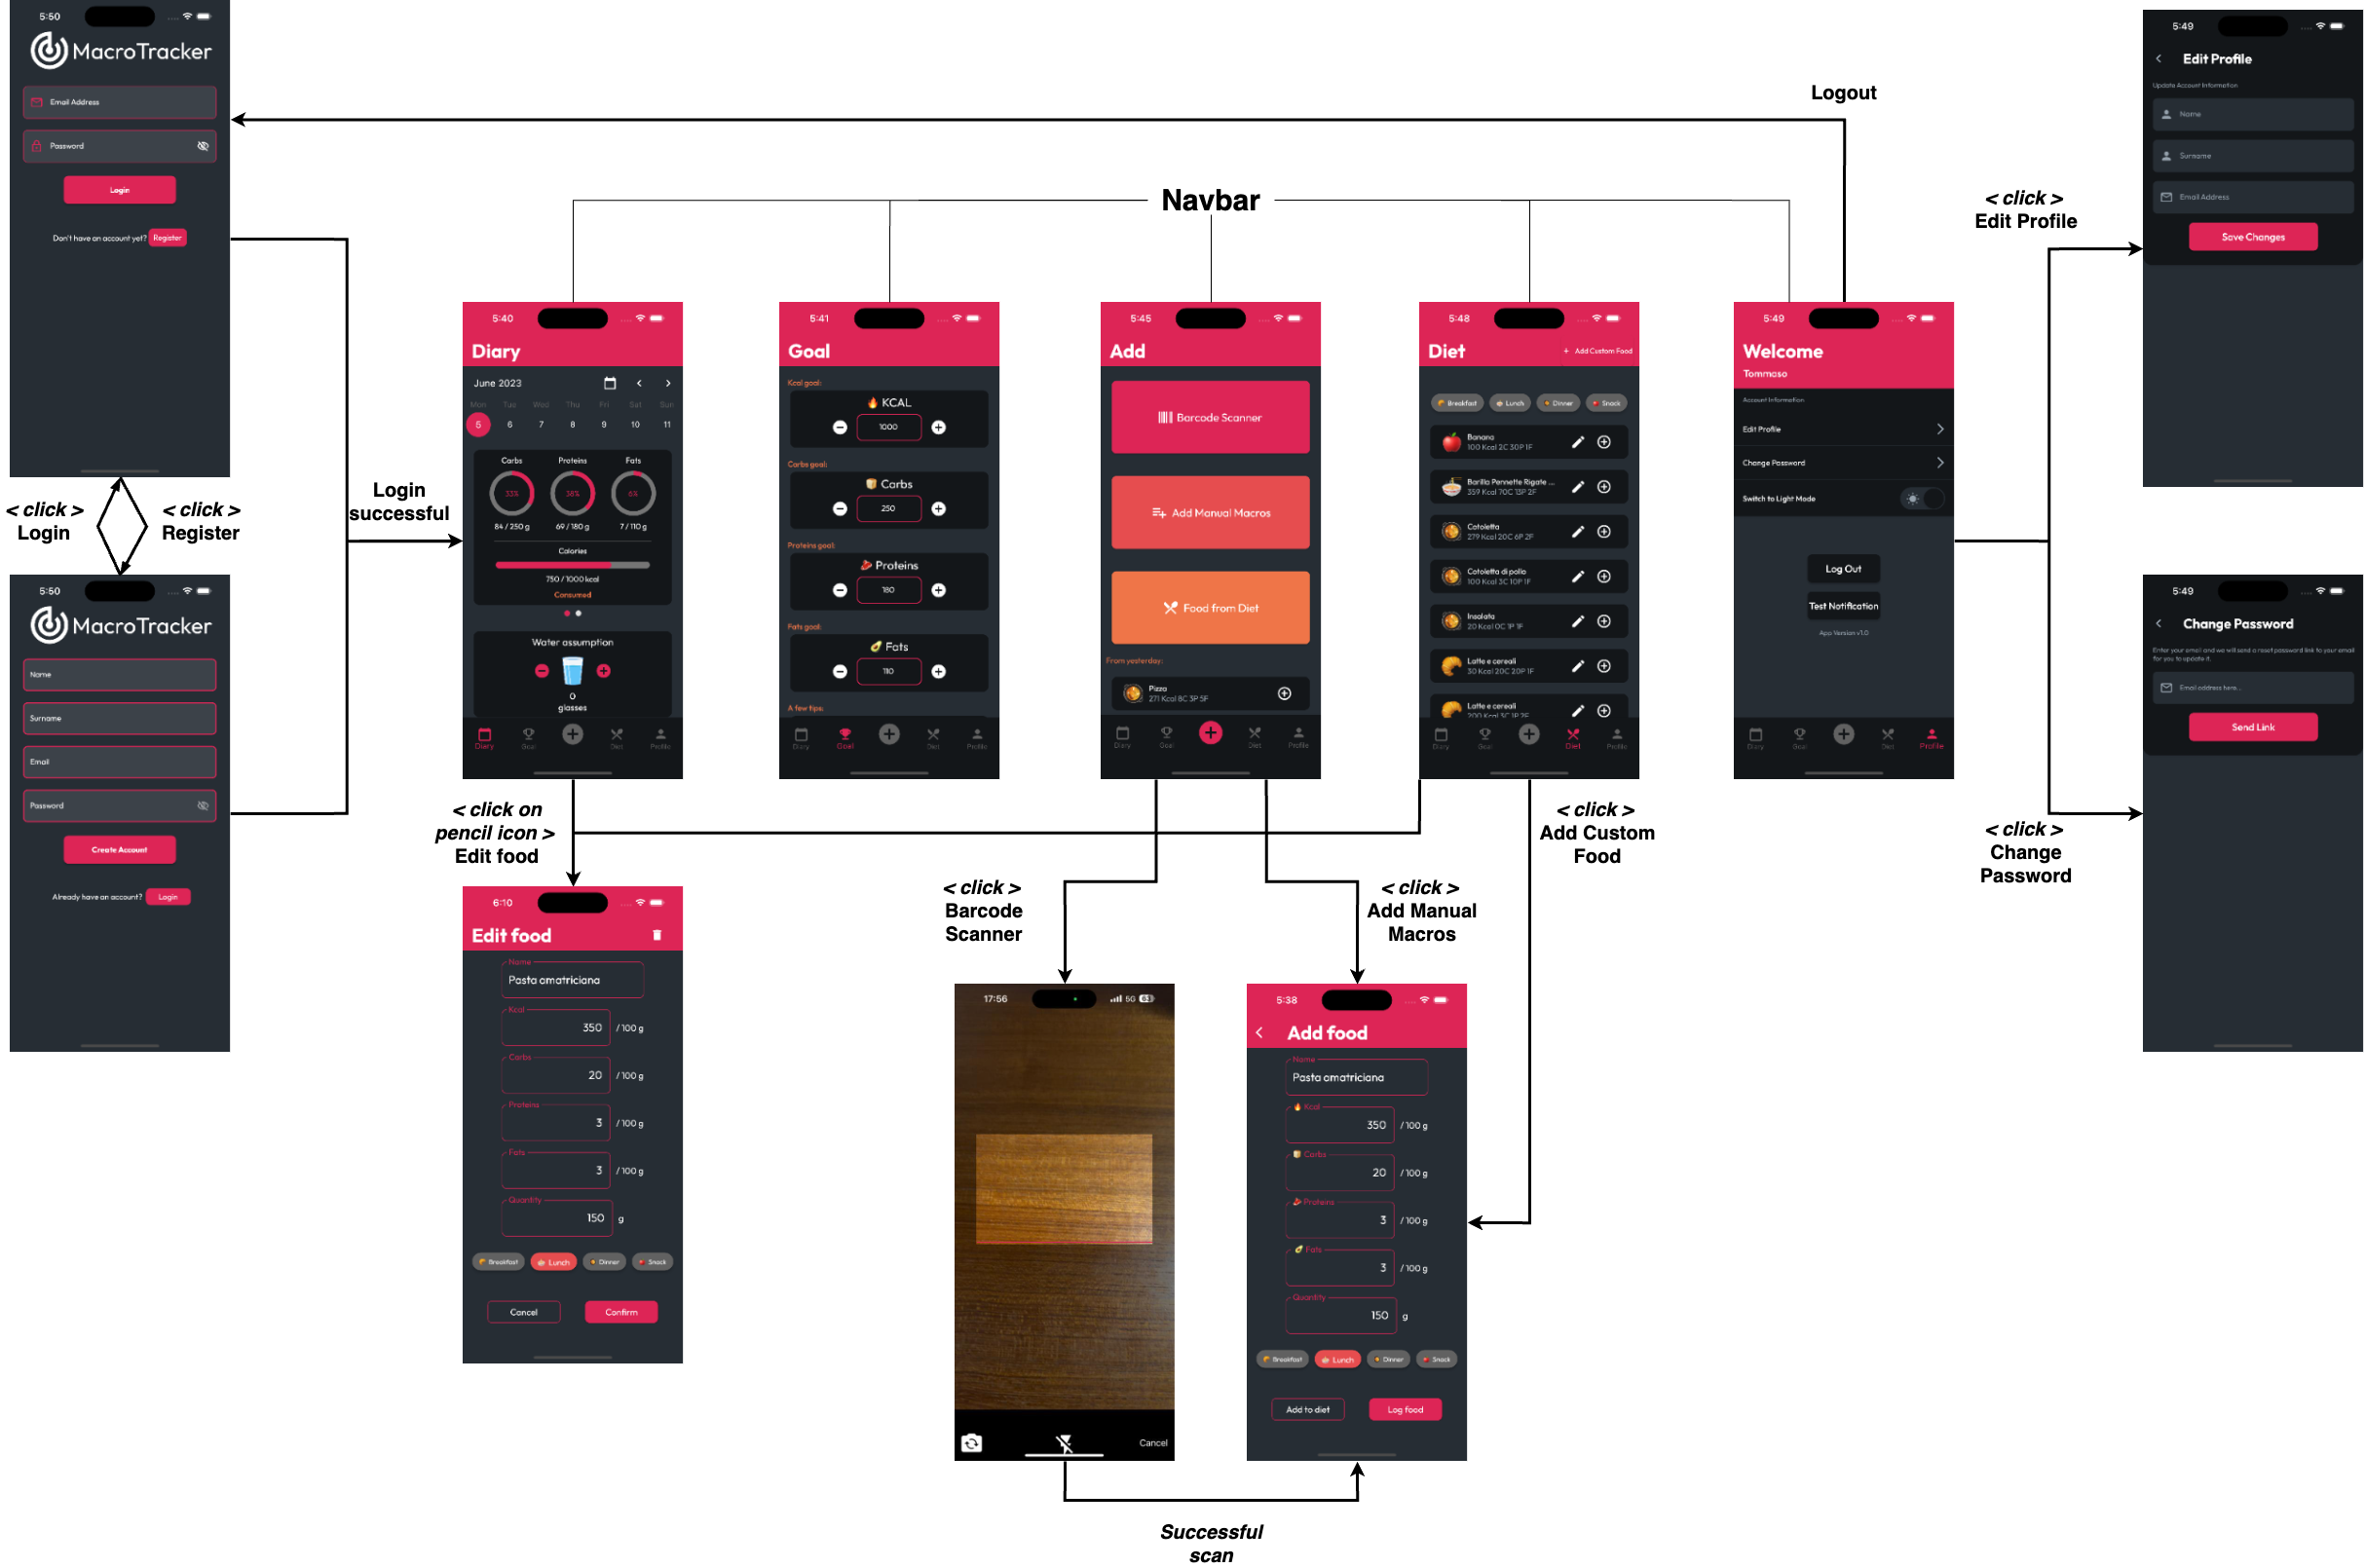
\includegraphics[scale=0.18]{Images/UX.png}
\end{figure}


\chapter{App Testing}
\section{Unit testing}
Most of the methods in the application involve either making API calls, to Firebase or to the previously described services, or organizing the screen's layout, making it inappropriate for unit testing.
\section{Widget testing}
To ensure successful testing, a \textit{mocked} version was developed for each widget in the app. These versions eliminate any Firestore queries and API calls that may lead to test failures, replacing them with static values. The primary objective of this testing approach is to confirm the presence of all expected sub-widgets within each widget's layout and validate that the displayed texts accurately match the statically inserted content.

\begin{longtable}{|m{3cm}|m{6cm}|m{5cm}|}
    \hline
     \multirow{2}{*}{\textbf{Widget tested}} & \multirow{2}{*}{\textbf{Description}} & \multirow{2}{*}{\textbf{Problems and notes}} \\[0.5ex]
        & \\[-1ex]
    \hline
    \endfirsthead
    \hline
    \centering
     \multirow{2}{*}{\textbf{Widget tested}} & \multirow{2}{*}{\textbf{Description}} & \multirow{2}{*}{\textbf{Problems and notes}} \\[0.5ex]
        & \\[-1ex]
    \hline
    \endhead
    \hline
    \endfoot
    \hline
    \endlastfoot 
    \textit{AddBarcodeFood Widget} & The test verifies that the widgets contain all the necessary \textit{TextFields} for inserting food, as well as the parent widgets that encapsulate them, along with the appropriate title in the \textit{AppBar}. & - \\
    \hline
    \textit{Add Widget} & Asserts the presence of the three buttons that enable the user to add food, along with the \textit{ListView} and the texts related to the foods inserted yesterday. Additionally, it verifies the correctness of the \textit{AppBar} and the parent widgets. & Since FlutterFlow was utilized in the implementation, certain widgets were not captured by the test, thereby preventing us from asserting their presence through this testing approach. \\
    \hline
    \textit{ChangePassword Widget} & The test case verifies the presence of a form specifically designed for users to enter their email address for password reset purposes. It further ensures the existence of the necessary text components that accompany the form. Additionally, the test validates the accuracy of the title widget and confirms that its displayed text content aligns with the expected values. & The presence of the button could not be asserted due to it being implemented as a FlutterFlow (FF) widget. \\
    \hline
    \textit{Diary Widget} & Asserts the presence of the Calendar, while also meticulously verifying the exact number of \textit{LinearPercentIndicator} and \textit{CircularPercentIndicator} elements representing the user's progress. Additionally, it ensures the availability and functionality of the adding/removing buttons for water glasses and coffee cups. Moreover, it examines and confirms the correct display of manually inserted texts across all pages, assuring the accuracy and consistency of the displayed content. & Several overflow size exceptions were encountered during the testing phase, primarily attributed to the boxes that encapsulate the percentage indicators. These exceptions arose due to the content exceeding the available space allocated for display, leading to visual anomalies and irregularities in the layout.  \\
    \hline
    \textit{Diet Widget} & The test case asserts the presence of the parent sub-widgets and verifies the existence of the \textit{ListView}, which displays a mock list of foods for testing purposes. Furthermore, it ensures the correct rendering of the title in the \textit{AppBar}. & The verification of the \textit{ChoiceFilter} widget's presence was not feasible, primarily due to its implementation as a FlutterFlow (FF) widget. \\
    \hline
    \textit{EditFood Widget} & The test ensures the presence of the necessary text fields for editing the food, including the corresponding deletion icon and other relevant parent widgets. Furthermore, like for the other tests, it specifically checks for the exact matching of the page title in the \textit{AppBar}. & - \\
    \hline
    \textit{EditProfile Widget} & The test asserts the presence of the form to be compiled to edit the user profile, and the corresponding text displaying the UI of this page. &  - \\
    \hline
    \textit{Goal Widget} &  The test verifies the presence of all the sub-widgets that displays the widget, including the precise number of text fields for modifying the goal and the corresponding buttons for increasing or decreasing the goal values. Additionally, it expects to locate the \textit{PageView} component that pertains to the tips provided for standard goals. Furthermore, the test examines the texts positioned above the text fields and ensures that the text initially populated within the fields aligns with the expected values. & Some overflow exceptions arose with the page, which have been resolved by incorporating a \textit{SingleChildScrollView}. This ensures that all sub-widgets are displayed correctly across various screen formats. \\
    \hline
    \textit{Login Widget} & The test primarily verifies the presence of the forms for inserting the user's email and password. Furthermore, it ensures the correct display of the app's name and logo icon. Additionally, it checks for the proper rendering of other helpful UI texts. & Similar to the previously described tests, this test was unable to directly verify the presence of button widgets. However, this challenge was overcome by examining the text content within those buttons. \\
    \hline
    \textit{Profile Widget} & This test verifies the presence of all the necessary widgets required for profile management. It includes checking for the presence of the \textit{InkWell} widget responsible for creating the row that displays various options. Additionally, it ensures the presence of the sub-widgets that compose the page. The test also verifies the correctness of all statically inserted texts within the mocked widget. & - \\
    \hline
    \textit{Register Widget} & Similar to the Login Widget test, this test verifies the presence of the required sub-widgets in the Register Widget. It ensures that the widget contains four forms for user input, including fields for the user's name and surname. The goal is to validate that all the necessary components are present for successful user registration. & -\\
    \hline
    \caption{Widget tested in widget testing.}
\end{longtable}

\section{Integration testing}
The integration testing has been performed by the usage if two flutter packages:
\begin{itemize}
    \item \text{flutter\_test/flutter\_test.dart}
    \item \text{integration\_test/integration\_test.dart}
\end{itemize}
The objective of this type of testing is to simulate user behavior within the app. Specifically, the tests described below navigate through different screens starting from the main Diary Widget and simulating user interactions to verify the expected outcomes.
\\
Note: Before proceeding with each test, the presence of the sub-widgets in the starting widget is verified. Similarly, after the navigation, the presence of the sub-widgets in the final destination is confirmed.

\begin{longtable}{|m{6cm}|m{6cm}|}
    \hline
     \multirow{2}{*}{\textbf{Screen navigation tested}} & \multirow{2}{*}{\textbf{Description}} \\[0.5ex]
        & \\[-1ex]
    \hline
    \endfirsthead
    \hline
    \centering
     \multirow{2}{*}{\textbf{Screen navigation tested}} & \multirow{2}{*}{\textbf{Description}} \\[0.5ex]
        & \\[-1ex]
    \hline
    \endhead
    \hline
    \endfoot
    \hline
    \endlastfoot 
    \textit{Add screen} & This test consists of three sub-tests. The first sub-test focuses on navigating from the \textit{Diary} screen to the \textit{Add} screen. In the second sub-test, while being in the \textit{Add} screen, it simulates a click on the \textit{Add Manual Macros} button. This action is performed to navigate to the \textit{AddFood} screen and verify that the user is effectively on that page. The last sub-test is similar to the second one, but it clicks on the \textit{Food from Diet} button instead. Overall, this test ensures successful navigation to the \textit{Add} screen and thoroughly tests all the buttons that lead to other pages. \\
    \hline
    \textit{Diet screen} & This test verifies the navigation from the the \textit{Diary} screen to the \textit{Diet} screen. Then, by simulating a click on the "pencil" icon, it asserts the correct navigation to the \textit{EditFood} screen.\\
    \hline
    \textit{Goal screen} & This test verifies the navigation from the \textit{Diary} screen to the \textit{Goal} screen. Then, it statically inputs the value "2000" in the kcal text field. After that, it simulates two clicks: one on the "plus" icon next to the corresponding field to verify that the value increases and is correctly displayed as "2050", and one on the "minus" icon to decrease the value, confirming the correct behavior of all the involved widgets. \\
    \hline
    \textit{Profile screen} & This test verifies the navigation from the \textit{Diary} screen to the \textit{Profile} screen. After that, ensuring that the app is in the default light mode, it simulates a click on the theme mode switch and asserts the expected theme change. \\
    \hline
    \caption{Screens tested in navigation testing.}
\end{longtable}

\section{User testing}
The app has undergone extensive testing on both student devices and emulators throughout the entire development process. During these daily tests, various graphical, logical, and backend bugs were identified and resolved on a day-to-day basis.

One notable issue that arose was related to the insertion of values into text fields, particularly those within the \textit{Goal} widget. This problem occurred due to the simultaneous update of values in both the app and the Firestore database.

All bugs and problems discovered were promptly communicated to each other member of the group in real-time, ensuring that everyone was aware of the issues and that they were resolved as quickly as possible.

In order to replicate the user experience, the app was utilized and tested for a duration of two weeks, allowing for thorough evaluation.

\chapter{Effort spent}

\begin{table}[h]
\begin{adjustwidth}{-2cm}{}
\begin{tabular}{|m{3.5cm}|m{2cm}|m{1.5cm}|m{1.5cm}|m{3.1cm}|m{3cm}|m{1.5cm}|}
\hline
\textbf{Student} & \textbf{Database} & \textbf{Design} & \textbf{App} & \textbf{Documentation} & \textbf{Presentation} & \textbf{Total} \\
\hline
Alessandro Sironi & 2h & 40h & 100h & 5h & 3h & 150h\\
\hline
Tommaso Sprocati & 4h & 40h & 100h & 5h & 1h & 150h\\
\hline
\end{tabular}
\end{adjustwidth}
\end{table}


\end{document}
